\documentclass[12pt]{report}

% lacunae etc indicated by FIX
% places which need to be checked for current 
% truth are indicated by UPDATE

\usepackage{latexsym}
\usepackage{times}
\usepackage{mathptm}
% use the time fonts for better results with
% pdf (CM fonts don't index correctly)

\ifx\pdfoutput\undefined
  \usepackage[dvips]{hyperref}
\else
  \usepackage[pdftex,colorlinks,pdfstartview=Fit,b5paper]{hyperref}
  \pdfinfo{ 
    /Title (The (new) LKB system) 
    /Author (Ann Copestake)
    /Subject ()
    /Keywords ()
  }

\pagestyle{empty}

\setlength{\paperwidth}{8in}
\setlength{\paperheight}{6in}
\setlength{\textwidth}{7in}
\setlength{\textheight}{5in}
\setlength{\topmargin}{-1in}  
\setlength{\evensidemargin}{-.5in}
\setlength{\oddsidemargin}{-.5in}
\fi

\usepackage{graphicx}

%- comment out epsf box for TeXtures
%\input epsf
%\newcommand{\epsfbox}[1]{}
%\def\epsfxsize{}
\input thedefs1
%\input thedefs

%\setlength{\evensidemargin}{0in}
%\setlength{\oddsidemargin}{0in}
%\setlength{\textwidth}{6.5in}
%\setlength{\topmargin}{-0.5in}
%\setlength{\textheight}{9in}




\newcommand{\itsdb}{{\sf \lbrack incr tsdb()\rbrack}}

\newcommand{\lispcommand}[1]{\noindent\textrm{#1}}%
\newcommand{\ldescnl}{\\}
\newenvironment{error}%
{\begin{quote}
\tt
}%
{\end{quote}
}
\newenvironment{warning}%
{\begin{quote}
\tt
}%
{\end{quote}
}

\newcommand{\filename}[1]{\texttt{#1}}
\newcommand{\functionname}[1]{\texttt{#1}}
\newcommand{\lkbentryname}[1]{\texttt{#1}}
\newcommand{\lkbparam}[1]{\texttt{#1}}
\newcommand{\lkbmenucommand}{{\bf}}
\newcommand{\newterm}[1]{\emph{#1}}

% commands for figures
\newcommand{\figtype}[1]{\textbf{\strut #1}}
\newcommand{\figfeat}[1]{\textsc{\strut #1}}
\newcommand{\nodedot}{\circle*{5}}

%\newcommand{\semnest}[1]{AVM omitted because of semantic nest size}
\newcommand{\semnest}[1]{#1}

\begin{document}
\vspace*{.5in}
\begin{center}
{\Huge\bf The (new) LKB system}\\[0.2in]
Version 5.2\\%[0.2in]
\today\\[0.2in]%[1in]
system development by\\[0.2in]
{\Large Ann Copestake, John Carroll, Rob Malouf, Stephan Oepen\\ 
and others}\\[0.5in]
documentation (mainly) written by\\[0.2in]
{\Large Ann Copestake}\\
{\tt aac@csli.stanford.edu}\\[0.5in]
\end{center}
\vfil
This document describes the new version of the LKB system:
a grammar and lexicon development environment for use with
constraint-based linguistic formalisms.
\clearpage

\tableofcontents

\chapter{Introduction}

\section{A brief introduction to the LKB system}

The LKB (Linguistic Knowledge Building)
system is a grammar and lexicon development environment for use with
constraint-based formalisms.\footnote{Development 
of the LKB system was originally supported by ACQUILEX projects
BRA-3030 and 7315 under the Esprit program.  More recent research
has been supported by the
National Science Foundation under grant number IRI-9612682.
Detailed acknowledgments are in \S\ref{ack}.}
It is specifically designed for the use of typed
feature structures.  It is intended to be used for Natural Language Processing
research involving unification-based linguistic formalisms for parsing and/or
generation, and also for teaching.  It has been most extensively tested with
grammars based on HPSG (Pollard and Sag, 1987, 1994), but it is intended to be
framework independent.  In this philosophy, and in much else, 
we have tried to follow PATR
(Shieber, 1986).  The LKB system is implemented in Common Lisp and the
basic system is intended to 
run on any Common Lisp implementation, although the
graphical environment is currently limited to Macintosh Common Lisp (MCL)
or Allegro Common Lisp with the Common Lisp Interface
Manager (CLIM).\footnote{{\bf MCL} and 
{\bf Macintosh Common Lisp} are trademarks of Digitool, Inc.
{\bf Macintosh} is a trademark of Apple Computer.
{\bf Allegro CL} is a trademark of Franz Inc.
All other trademarks used in this document are the property of their
owners.}
Sites without a Lisp license that have suitable hardware can 
also use the LKB system:
for details of hardware requirements and installation, 
see Chapter~\ref{installation}.

The best way to think about the LKB system, and other comparable systems such
as \href{http://www.sfs.nphil.uni-tuebingen.de/~gpenn/ale.html}{ALE} 
and \href{http://www.dfki.de/lt/systems/page/page.html}{PAGE}, 
is as a development environment for a very high-level
specialized programming language.  Typed feature structure
languages are essentially based on one data structure --- the typed feature
structure, and one operation --- unification.  This combination is powerful
enough to allow the grammar developer to write grammars and lexicons that can
be used to parse and generate natural languages.  In effect, the grammar
developer is a programmer, and the grammars and lexicons 
comprise code to be run by
the system.\footnote{From now on, we'll use grammar to mean
all the linguistic code: that is grammar rules, lexicon, lexical rules 
and so on.}  
But because the typed feature structure language 
is so high level, working in it requires relatively little knowledge
of computers.  Typed feature structure languages were designed
(by linguists) as a formal way of specifying linguistic
behaviour rather than as programming languages, and they are used
in this way by people who have no involvement in computational 
linguistics.  So, at least potentially, these languages have several
advantages: they make computational
linguistics and natural language processing accessible to linguists
with a very limited background in computers, they enable computational 
linguists to adopt techniques from theoretical linguistics with minimal 
reinterpretation, and they allow formal theories to be tested on
a range of data in a way that allows the interaction between
treatments to be checked.

The LKB system is therefore a software package for writing
linguistic programs, i.e., grammars, and it's
important not to confuse the system and the grammars which run on it. By
itself the LKB system is of no use in an application, since
there has to be some associated grammar.
Although we distribute some grammars with the LKB, they are 
primarily there to act as
examples, just as programming language packages include example code.  
The LKB system can be used to develop many different grammars.
What's more,
a grammar developed on the LKB system could in principle
be run on another platform that used the same typed feature 
structure language, just as a C$++$ program can be run
by a variety of compilers.\footnote{In practise, however, there
is no agreed standard for typed-feature structure systems.
The current situation is roughly similar to the different Lisp implementations
which existed before Common Lisp was initially developed, which is
to say that some grammars can be converted relatively easily between
platforms, while others are extremely difficult to convert because 
they use facilities which are not shared by all typed feature structure
based systems.  For example, the LKB system uses a version of 
default unification
which is not available on other typed feature structure systems,
and so grammars which use defaults are less portable than ones which
don't.  It's unlikely that there will ever be an ANSI-standard
typed feature structure language, though developers of the different
systems are trying to make portability easier, so the situation should
improve in the near future.}  
The performance of the LKB system in tasks such
as parsing depends critically on the grammar: it makes little sense to 
talk about performance except with respect to a 
particular grammar.  We have, however, tried to make it reasonably efficient
with fairly large grammars.

The LKB system
must therefore be distinguished from the LinGO English resource grammar
(ERG) which is also being developed at CSLI.  The LinGO ERG runs on 
several systems beside the LKB, including PAGE.
The ERG is being distributed in parallel with the LKB system,
but is not discussed in this documentation.  However
some examples of the ERG are used here in order
to illustrate some of the facilities the system has for dealing 
with large and complex grammars.

\section{This manual}

The purpose of this manual is to teach users how to use the LKB system
to program their own grammars or to adapt existing ones.
We have tried not to make too many assumptions
about what the user knows how to do, but there are some things we have 
to assume if the documentation is ever going to be finished.
With respect to the content of the system, we've tried to write the 
documentation so that a user can start building grammars even if
they have never used a grammar development environment before,
and we have provided a chapter which is a non-technical introduction
to typed feature structure formalisms,
but we do not try and cover any linguistic theory.
Some of the grammars distributed with the LKB are
linked to a textbook which introduces
formal syntax using a typed feature structure
formalism: Sag and Wasow (1999).
There are some places where to fully understand
the documentation a knowledge of some NLP concepts, such as chart parsing,
will be helpful, but this should not be essential to use the system.
On the interaction side,
we assume the user knows how to open, close, resize windows etc
and how to select menu items.  We also assume that the user knows
how to use emacs, at least at a fairly elementary level, if running
the ACL/CLIM version of the LKB, or the MCL editor, if using a Mac.
There are a couple of places where it's useful to have a 
very basic understanding of Common Lisp, in particular when installing the
system, but we've tried to avoid this being essential.
 
The rest of this chapter contains a few more brief details
of the LKB system and how it has been developed.
The following chapter describes installation of the LKB.
The third chapter
is intended for first time users: it gives
a fairly detailed tour through some of the LKB's functionality.
The fourth chapter is a basic
and informal introduction to typed feature structures.
Chapter~\ref{formal} contains a formal description
of typed feature structures as used in the LKB.
The subsequent chapters are the reference manual proper --- they
are not intended to be read straight through, but to act as 
a source of information about error messages,
user interface commands which have less than
obvious behaviour and so on.
The first of these chapters
covers the
file organization, loading, error messages and so on.  The
next describes the user interface.  The last chapter
covers `advanced' features: generally speaking, this can be
ignored by people who are adapting an existing grammar.
The appendices cover details of the
available parameters and other details which most readers probably
do not wish to know about.

\section{Some history}

Initially the LKB system was developed on the 
EU-funded ACQUILEX project primarily as a
tool to allow the construction of typed feature structure based lexicons
(both monolingual and bilingual).\footnote{At this point, LKB stood for
Lexical Knowledge Base --- the LKB system was a tool for building
LKBs.} 
Although it incorporated a parser,
this was of secondary importance, since it was mostly intended as
a way of verifying lexical entries.  The most extensive documentation
of that version of the system is Copestake (1993): published
papers include Copestake (1992) and several papers in Briscoe et al (1993).
The current version of the LKB has 
been extensively updated.  Some of the main changes compared to the older
version are:
\begin{enumerate}
\item Extensive efficiency improvements, so the system is capable
of parsing reasonable length sentences with a large grammar.
\item Default unification is based on YADU, defined in Lascarides and
Copestake (1999).
\item Automatic computation of greatest lower bounds in the type hierarchy.
\item Integration with the \itsdb\footnote{This is really
what the system is called, but this is not
the responsibility of the current author.  Please direct any comments
about \itsdb\ to {\tt oe@coli.uni-sb.de}.}\ test suite machinery 
(Oepen and Flickinger, 1998).
\item Integration with MRS semantics (Copestake et al, 1999).
\item Tactical generation from MRS input (relatively experimental). 
\item Many new user interface features.
\end{enumerate}
Some of the earlier functionality has not made it into the new version:
either because the developers consider it obsolete or simply because of
shortage of time.  

\section{Acknowledgments}
\label{ack}

The main developers of the LKB system 
are Ann Copestake, John Carroll, Rob Malouf and Stephan Oepen.  
The distributed system also incorporates code
written by Bernie Jones, Dan Flickinger and   
John Bowler.  Ted Briscoe and Antonio Sanfilippo had a great 
deal of influence on the design of the original system,
Dan Flickinger played a similar role for the new version.
Uli Callmeier has done extensive testing and uncovered numerous
bugs and infelicities.
Invaluable input has also
been provided by users too numerous to thank individually, including
researchers on the ACQUILEX and LinGO projects, at
the Copenhagen Business School and Edinburgh University,
students
at the University of Cambridge Computer Laboratory and
Stanford University and students on a course taught by Copestake, Flickinger
and Oepen at ESSLLI-98.  Special thanks go to
Matt Kodama, Ryan Ginstrom, Christopher Callison-Burch, Scott Guffey
for their detailed comments on design and extensive testing.


\chapter{Installing and running the system}
\label{installation}

This chapter gives details of downloading, installing and 
starting up the LKB system.
CSLI users can skip to \S\ref{run-csli} (most users) or \S\ref{down-csli}
(users who are editing Lisp code).
Other users will need to look at the next section to decide in
what form to download the system, then go through the steps in the
other sections, depending on their 
choice.

\section{Hardware and software requirements}
\label{require}

The LKB system is freely available for teaching, research or commercial use,
though we retain copyright:
the conditions placed on redistribution are described on the 
\href{http://www-csli.stanford.edu/~aac/lkb.html}{LKB Web Site}.
We encourage users to make enhancements and upgrades to the system,
and will be happy to make any improvements available from the Web site.

The full LKB system is available in a variety of configurations:
\begin{enumerate}
\item Solaris image for the Sparc architecture (using Allegro Common Lisp)
\item Linux image for Intel x86 architecture (using Allegro Common Lisp)
%\item Mac image
\item Source files for Allegro Common Lisp and CLIM
\item Source files for Macintosh Common Lisp (MCL)
\end{enumerate}
Both images are made using Allegro Common Lisp and
can be run without a license, though since they do not contain
a Lisp compiler, anyone who wants to make any substantial
modifications to the
system will need a license from the Lisp vendor
so that they can work with the source files.

To use any version of the LKB, 
you need a machine with adequate amounts of memory.
We would suggest 32 Meg of RAM as a minimum on MCL, 
and 64 Meg for ACL with CLIM.
To run larger grammars
you will need larger amount of memory.  
The Solaris image should run on recent versions of SunOS.
The Linux image was made for Red Hat 6.0 with Metrolink Motif 1.2
(glibc version).  It should run on some other versions of Linux, but
is known not to be compatible with most other versions of Motif: 
please see the Franz Website.

If you have Allegro Common Lisp with CLIM or Macintosh Common Lisp, you 
can download the source files
and compile them.  This will be necessary
if you want to substantially
modify the LKB source code, and is likely to be
advantageous in any case, since we make minor bug fixes available
as source, rather than providing new images.
% UPDATE POINT
We have tested the curent version of the LKB
system on Allegro Common Lisp 5.0 on SunOS 5.6 
(with all patches installed)
and on Red Hat Linux 6.0 with Metrolink Motif 1.2
and (less extensively) on 
Macintosh Common Lisp 4.0.
It should work on other versions of these Lisps, but we are not in a position
to offer much advice in case of problems for Lisp/OS versions
we don't use.

If you do not have access to a machine for which we provide an image,
and do not have either Allegro Common Lisp with CLIM or Macintosh Common
Lisp, the LKB can still be run in `tty' mode from other Common Lisps.
tty mode is also useful if you are accessing a machine over a 
modem or a slow network
where the graphical display is impossible or would take too long.
In this mode, commands are entered by typing rather than menu selection,
and display commands result in ASCII output (or in some cases are
not available).
tty mode is described in detail in Appendix~\ref{tty}.

Some source code is available for 
the Windows version of Allegro Common Lisp (Common Graphics) but the port 
is incomplete and this will only be useful for someone who is prepared
to do substantial programming: please contact Ann Copestake for details.

For up-to-date information on what is available, check the 
\href{http://www-csli.stanford.edu/~aac/lkb.html}{LKB Web Site}
and/or subscribe to the LKB mailing list (see the website for instructions).
If you want to consider acquiring ACL/CLIM or MCL in order to run the source,
please see the links to the companies on the LKB web page.\footnote{We 
would be grateful if you let the vendor know if you intend to use the
system primarily for the LKB
and also let us know of any such purchase, since it allows us to
be more persuasive when it comes to requesting the vendors 
to fix bugs etc \ldots}

\section{Downloading the LKB}
\label{down}

\subsection{Downloading an image}
\label{down-images}

The image files for Linux and Sun Solaris are available from the
\href{http://www-csli.stanford.edu/~aac/lkb.html}{LKB Web Site}
as gzipped Unix tar files.
Download the appropriate file, making sure you are using binary mode.
Then:
\begin{verbatim}
gunzip climimage5-2.tar.gz
\end{verbatim}
or
\begin{verbatim}
gunzip linuximage5-2.tar.gz
\end{verbatim}
this should give you a file called \filename{climimage5-2.tar} or
\filename{linuximage5-2.tar}
Put this in a directory where you want the LKB system to reside
and extract the LKB image directory by:
\begin{verbatim}
tar xf climimage5-2.tar
\end{verbatim}
or
\begin{verbatim}
tar xf linuximage5-2.tar
\end{verbatim}
This will create the new directory called \filename{lkb} containing
several files. 

Also download the data files, and unzip etc in the same way:
\begin{verbatim}
gunzip data5-2.tar.gz
tar xf data5-2.tar
\end{verbatim}
This will create a new directory tree called \filename{data} containing
various sample grammars.

Now follow the instructions in \S\ref{emacs-clim-image}
or \S\ref{clim-image}
%or \S\ref{mcl-image} 
to start the LKB.


\subsection{Downloading source files}
\label{down-src}

The source files are distributed as a 
gzipped Unix tar file which is available from the
\href{http://www-csli.stanford.edu/~aac/lkb.html}{LKB Web Site}.
A single file is used for all systems, since most of the code is shared.
Download the file, making sure you are using binary mode.
Then:
\begin{verbatim}
gunzip lkbsrc5-2.tar.gz
\end{verbatim}
this should give you a file called \filename{lkbsrc5-2.tar}.  
Make sure this in a directory where you want the LKB system to reside
and extract the LKB by:
\begin{verbatim}
tar xf lkbsrc5-2.tar
\end{verbatim}
This will create the new directory and various subdirectories.
It may take a few minutes to do this.  At this point, you have 
your own local copy of the LKB system source.  Note that
you may need to change the directory locations in \filename{general/loadup}
and \filename{main/userfns}
to be appropriate for your system
(especially if you wish to run the system using MCL).

Also download the data files, and unzip etc in the same way:
\begin{verbatim}
gunzip data5-2.tar.gz
tar xf data5-2.tar
\end{verbatim}
This will create a new directory tree called \filename{data} containing
various sample grammars.

Now follow the instructions in \S\ref{acl-src} or \S\ref{mcl-src}
to compile the files.

\subsection{Running the LKB at CSLI}
\label{run-csli}

To run the LKB on eo or the linear machines
follow the instructions in \S\ref{acl-emacs} 
(\functionname{fi:common-lisp} is already installed)
but give the file \filename{/usr/acl/lkb} 
in response to the prompt for {\bf Executable image name:}

\subsection{Getting a local copy of the LKB source at CSLI}
\label{down-csli}

In order to get a local copy of the LKB source at CSLI, you need to
checkout the latest version from the cvs system.  To do this,
you must have access to eo or one of the linear machines.  
You will also need filespace
on these machines.

First make sure that the CVSROOT enviroment variable is set.  You probably want
to put the following in your \filename{.login} file, or you can just type it
into the shell.
\begin{verbatim}
setenv CVSROOT /eo/e1/CVSROOT
\end{verbatim}
In the directory which you wish to act as the root for the LKB source
(your home directory is fine), execute the following:
\begin{verbatim}
cvs checkout newlkb
\end{verbatim}
This will create the new directory and various subdirectories.
It may take a few minutes to do this.  At this point, you have 
your own local copy of the LKB system.  Instructions on using
cvs are on the CVS Website:
\href{http://www.loria.fr/~molli/cvs-index.html}{http://www.loria.fr/~molli/cvs-index.html}.

Now follow the instructions in \S\ref{acl-src} to compile the
files, and in \S\ref{acl-emacs} to start the LKB system from within
emacs.


\section{Compiling the source files}
\label{src}

\subsection{Allegro Common Lisp and CLIM (ACL/CLIM)}
\label{acl-src}

To compile the LKB system files in ACL/CLIM, do the following:
\begin{enumerate}
\item cd to \filename{newlkb/src}.  
\item Start ACL/CLIM.  The command needed will vary with your local
installation.  For instance,
at CSLI, the command to start ACL with CLIM is 
\filename{/usr/acl/base}.
\footnote{Note that since the objective is just to compile the system,
we describe the procedure for
starting the system from the command line.  For actually running the LKB,
it is preferable to start Lisp from within emacs, as described
in \S\ref{acl-emacs}.  If you prefer, you can follow the steps described
there, replacing the \functionname{load-system} command with 
\functionname{compile-system},
as below.}
\item At the Lisp prompt enter:
\begin{verbatim}
(load "general/loadup") 
\end{verbatim}
\item Once the loadup files have been loaded, enter the following:
\begin{verbatim}
(compile-system "lkb" :force t)
\end{verbatim}
This compiles and loads all the LKB files that are appropriate for
your system.\footnote{There may be
some warning messages --- these can usually be ignored, but if you subsequently
have problems using the LKB, you should redo this process
and examine the warning messages.}
If you intend to use any of the MRS code, including the generator,
you should replace \verb+"lkb"+ with \verb+"mrs"+: i.e.,
\begin{verbatim}
(compile-system "mrs" :force t)
\end{verbatim}
In either case, you
should now see the LKB interaction window, as shown in 
Figure~\ref{lkbtop-unix}.
\item At this point, you may simply exit Lisp:
you can restart the system from the compiled files
as described in \S\ref{acl-emacs}.
\end{enumerate}


\subsection{Macintosh Common Lisp (MCL)}
\label{mcl-src}

To compile the LKB system files do the following:
\begin{enumerate}
\item Double-click on the MCL icon to start MCL
\item If the LKB files are somewhere other than \filename{Macintosh HD:newlkb}
(e.g., because your hard disk is not called
\filename{Macintosh HD}),
open the \filename{src:general:loadup.lisp} file (Open is in the File menu 
in MCL) and edit the definition of \verb+%sys-home%+ to be appropriate
for your machine.  For instance, if your hard disk is called \filename{carrot},
and you want to use the folder name \filename{lkb5.2}
rather than \filename{newlkb},
the definition would look like:
\begin{verbatim}
(defparameter %sys-home%
  #-:mcl (rest (butlast 
                (pathname-directory *load-truename*) 2))
  #+:mcl '("carrot" "lkb5.2"))
\end{verbatim}
Save the file.
You may also need to edit the file \filename{src:main:user-fns.lsp} to
change the function definition of \functionname{lkb-tmp-dir} which refers to
\filename{Macintosh HD}.  These are the only places where you should need to
change file names.
\item Use the Load menu option to load \filename{newlkb:src:general:loadup}
\item Once the loadup files have been loaded, enter the following into the
Listener window:
\begin{verbatim}
(compile-system "lkb" :force t)
\end{verbatim}
If you intend to use any of the MRS code, including the generator,
you should replace \verb+"lkb"+ with \verb+"mrs"+: i.e.,
\begin{verbatim}
(compile-system "mrs" :force t)
\end{verbatim}
This compiles and loads all the LKB files that are appropriate for
your system.\footnote{There may be
some warning messages --- these can probably be ignored, but if you subsequently
have problems using the LKB, you should examine the
warning messages.}
You
should now see LKB on the menu-bar.
\item
At this point, you may simply exit Lisp:
you can restart the system from the compiled files
as described in \S\ref{mcl-comp}.
\end{enumerate}


\section{Running the LKB from compiled files}
\label{compiled}


\subsection{ACL/CLIM with emacs}
\label{acl-emacs}

To use the LKB commands for interacting with source files in ACL/CLIM, you must
use the emacs text editor and run a command that allows the linkage.  We
suggest the use of \functionname{fi:common-lisp} which is available from
\href{ftp: //ftp.franz.com/pub/emacs/eli/eli-2.0.21.16.2/}{ftp:
//ftp.franz.com/pub/emacs/eli/eli-2.0.21.16.2/}.  The following instructions
assume that this is installed on your system.  You can run the LKB from emacs
in a shell using the standard emacs commands, or you can start lisp with the
emacs function \functionname{run-lisp}, but the commands to show the grammar
files will not work.

\begin{enumerate}
\item The first time you use the system,
add the following lines to the bottom of your \filename{.emacs}
file, with the pathnames modified as appropriate for your
installation.
\begin{verbatim}

(if (not (member "/usr/acl/fi" load-path))
    (setq load-path (cons "/usr/acl/fi" load-path)))
(if (not (member "~/newlkb/src" load-path))
    (setq load-path (cons "~/newlkb/src" load-path)))
        
(load "fi-site-init")
(load "tdl-mode")
(load "lkb")
\end{verbatim}
\item The first time you run the system,
create a temporary directory (see \S\ref{tempdir}).  By default, this is
a directory called \filename{tmp} in your home directory.
\item Start emacs.  We will assume you
do this in the \filename{newlkb/src} directory.
\item Start ACL/CLIM from within emacs using the 
command \verb+fi:common-lisp+ which takes a number
of arguments. The
default values should be accepted with the exception
of the image name (the Lisp image appropriate for your
system should be specified), as follows:
\begin{quote}
\verb+M-x fi:common-lisp+\\
{\bf Buffer:} \verb+<RET>+\\
{\bf Host:} \verb+<RET>+\\
{\bf Process directory:} \verb+<RET>+\\
{\bf Executable image name:} \verb+/usr/acl/base+\\
{\bf Lisp image:}  \verb+<RET>+\\
{\bf Image arguments:}  \verb+<RET>+
\end{quote}
You should then get a new buffer called \verb+*common-lisp*+ with
a running Lisp process.  
\item At the Lisp prompt enter:
\begin{verbatim}
(load "general/loadup") 
\end{verbatim}
\item Once the loadup files have been loaded, enter the following:
\begin{verbatim}
(load-system "lkb")
\end{verbatim}
If you intend to use any of the MRS code, including the generator,
you should replace \verb+"lkb"+ with \verb+"mrs"+: i.e.,
\begin{verbatim}
(load-system "mrs")
\end{verbatim}
(If you haven't been following the instruction exactly, you may be asked whether
you want to compile some or all of these files.  Respond {\tt y} to this
question.)
\end{enumerate}
You
should now see the LKB interaction window, as shown in 
Figure~\ref{lkbtop-unix}.
To continue, see Chapter~\ref{firstsession}.
\begin{figure}
%\epsfbox[0 0 400 100]{figs/lkbtop-unix.ps}
\begin{center}
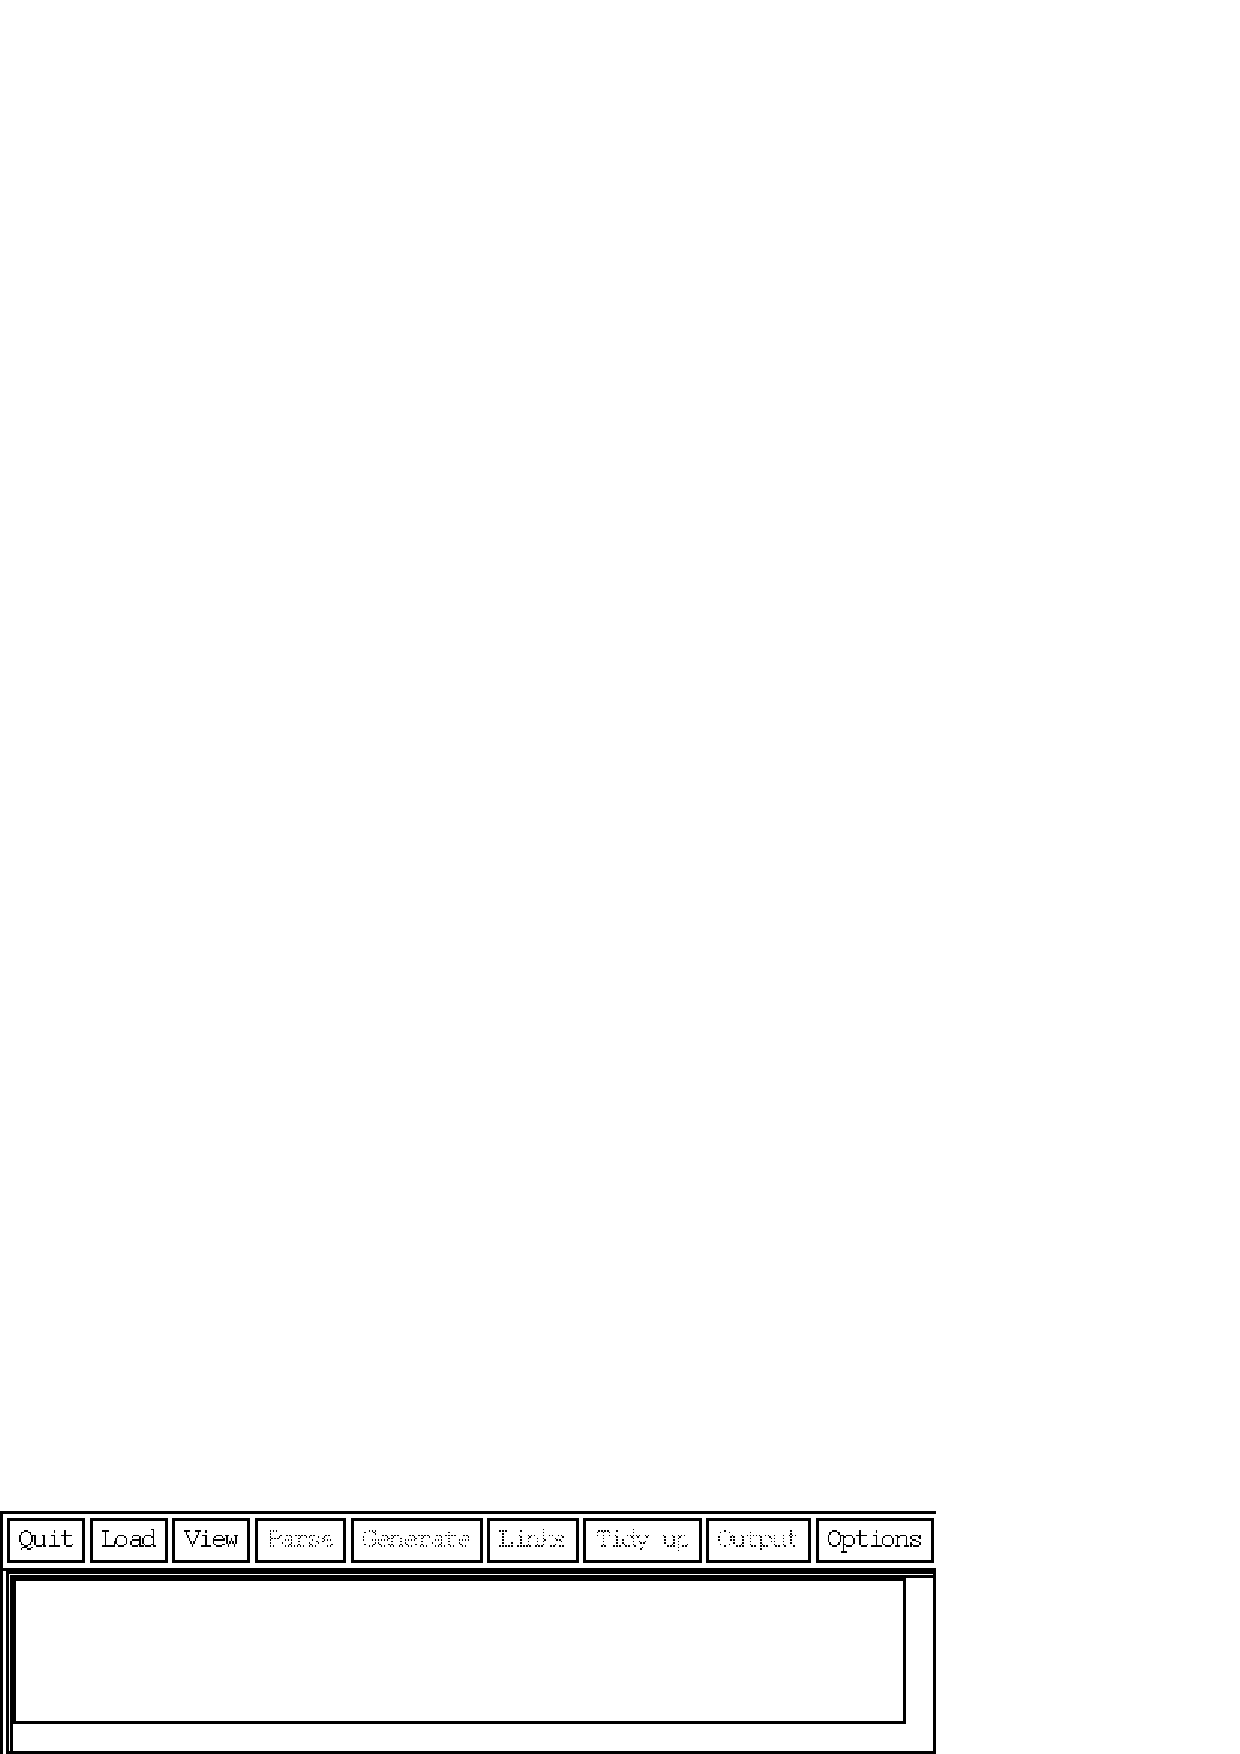
\includegraphics[width=400bp]{figs/lkbtop-unix}
\end{center}
\caption{The LKB interaction window in ACL/CLIM}
\label{lkbtop-unix}
\end{figure}

\subsection{ACL/CLIM without emacs}
\label{acl-comp}

If for some reason you cannot or do not wish to use
the LKB from emacs, you can start the LKB from compiled files as follows:
\begin{enumerate}
\item The first time you run the system,
create a temporary directory (see \S\ref{tempdir}).  By default, this is
a directory called \filename{tmp} in your home directory.
\item cd to \filename{newlkb/src}.  
\item Start ACL/CLIM as in \S\ref{acl-src}
\item At the Lisp prompt enter:
\begin{verbatim}
(load "general/loadup") 
\end{verbatim}
\item Once the loadup files have been loaded, enter the following:
\begin{verbatim}
(load-system "lkb")
\end{verbatim}
If you intend to use any of the MRS code, including the generator,
you should replace \verb+"lkb"+ with \verb+"mrs"+: i.e.,
\begin{verbatim}
(load-system "mrs")
\end{verbatim}
\end{enumerate}
You
should now see the LKB interaction window, as shown in 
Figure~\ref{lkbtop-unix}.
To continue, see Chapter~\ref{firstsession}.

\subsection{MCL}
\label{mcl-comp}

To start the LKB from MCL with compiled files, proceed as follows:
\begin{enumerate}
\item Create a temporary directory (see \S\ref{tempdir}).
\item Start MCL (double-click on the MCL icon)
\item At the Lisp prompt enter:
\begin{verbatim}
(load "general/loadup") 
\end{verbatim}
\item Once the loadup files have been loaded, enter the following:
\begin{verbatim}
(load-system "lkb")
\end{verbatim}
if you intend to use any of the MRS code, including the generator,
you should replace \verb+"lkb"+ with \verb+"mrs"+: i.e.,
\begin{verbatim}
(load-system "mrs")
\end{verbatim}
\end{enumerate}
You
should now see the LKB interaction menu on the menu-bar.
To continue, see Chapter~\ref{firstsession}.

\section{Running the LKB from an image}
\label{images}


\subsection{ACL/CLIM from emacs}
\label{emacs-clim-image}
To use the LKB commands for interacting with source
files in ACL/CLIM, you must use the emacs text editor with 
a command that allows the linkage.  We suggest
the use of \functionname{fi:common-lisp} which is available
from \href{ftp: //ftp.franz.com/pub/emacs/eli/eli-2.0.21.16.2/}{ftp: //ftp.franz.com/pub/emacs/eli/eli-2.0.21.16.2/}.  The following
instructions assume that this is installed on your system.
You can run the LKB from emacs in a shell using the standard
emacs commands, but the commands to show the grammar files
will not work.

\begin{enumerate}
\item The first time you use the system,
add the following lines to the bottom of your \filename{.emacs}
file, with the pathnames modified as appropriate for your
installation.
\begin{verbatim}

(if (not (member "/usr/acl/fi" load-path))
    (setq load-path (cons "/usr/acl/fi" load-path)))
(if (not (member "~/newlkb/src" load-path))
    (setq load-path (cons "~/newlkb/src" load-path)))
        
(load "fi-site-init")
(load "tdl-mode")
(load "lkb")
\end{verbatim}
\item The first time you run the system,
create a temporary directory (see \S\ref{tempdir}).  By default, this is
a directory called \filename{tmp} in your home directory.
\item Start emacs
\item Start the LKB from within emacs using the 
command \verb+fi:common-lisp+ which takes a number
of arguments.  If you have downloaded the image from our website
and stored it in the directory \filename{lkb}, accept all emacs's default
suggestions, with the exception of the {\bf Executable image name:}
as follows:
\begin{quote}
\verb+M-x fi:common-lisp+\\
{\bf Buffer:} \verb+<RET>+\\
{\bf Host:} \verb+<RET>+\\
{\bf Process directory:} \verb+<RET>+\\
{\bf Executable image name:} \verb+/lkb/lkb+\\
{\bf Lisp image:}  \verb+<RET>+\\
{\bf Image arguments:}  \verb+<RET>+
\end{quote}
You should then get a new buffer called \verb+*common-lisp*+ with
a running Lisp process (without a compiler, if you are using our
image).\footnote{If you get an error message concerning a missing library,
see \S\ref{problems}.}
\end{enumerate}
You
should now also see the LKB interaction window, as shown in 
Figure~\ref{lkbtop-unix}.
To continue, see Chapter~\ref{firstsession}.


\subsection{ACL/CLIM without emacs}
\label{clim-image}

If you cannot use emacs, or do not wish to for some reason,
simply start the saved image by running the executable
\filename{lkb} within the lkb directory (or whatever
other name you chose for it in the earlier stages).
You
should now see the LKB interaction window, as shown in 
Figure~\ref{lkbtop-unix}.\footnote{If 
you get an error message concerning a missing library,
see \S\ref{problems}.}
The first time you run the system, you should
create a temporary directory (see \S\ref{tempdir}).  By default, this is
a directory called \filename{tmp} in your home directory.
To continue, see Chapter~\ref{firstsession}.

\subsection{Macintosh}
\label{mcl-image}

If you are starting the LKB from a
Mac image, you simply double-click on the
icon for the image. 
You
should now see the LKB interaction menu on the menu-bar. 
The first time you run the system, you will need to
create a temporary directory (see \S\ref{tempdir}).
To continue, see Chapter~\ref{firstsession}.


\subsection{Temporary file locations}
\label{tempdir}

The LKB requires some temporary files be created for lexicon handling.  
Unfortunately, there is no way of ensuring that these will be created 
in a sensible place for every user on every Lisp system.
For
Unix, the default location for the
files is in a directory \filename{tmp} in the user's
home directory.  For MCL, the default location is \filename{Macintosh HD:tmp}.  If
it is possible to use these locations, then simply create the requisite
directory before loading the grammar.  If it is not convenient to have these
directories, if you are using source files, you can edit the file 
\filename{main/user-fns.lsp} 
so that the function \functionname{lkb-tmp-dir} identifies a more
suitable directory.  If you are using a supplied image file, you need to add a
\functionname{lkb-tmp-dir} 
function to the \filename{user-fns} file to be loaded by every grammar 
you use.  For instance,
if your Mac has a disc called \filename{Applications}, add the following
to the \filename{user-fns} file (or replace 
\functionname{lkb-tmp-dir} if it exists
already):
\begin{verbatim}
(defun lkb-tmp-dir nil 
  (let ((pathname  
          #-mcl (user-homedir-pathname)
          #+mcl (make-pathname :directory "Applications"))
        (tmp-dir '("tmp")))
    (make-pathname
     :host (pathname-host pathname) 
     :device (pathname-device pathname)
     :directory (append (pathname-directory pathname) tmp-dir)
     :name (pathname-name pathname) 
     :type (pathname-type pathname)
     :version (pathname-version pathname))))
\end{verbatim}

\section{Building an image}

If you wish to make a development image, for instance because
you want to make the LKB available for several users at your site,
this section gives brief instructions.

\subsection{Allegro Common Lisp}

To build an image, see the file \filename{ACL\_specific/image.lsp}.  This should
be loaded into a fresh Lisp image, after loading \filename{general/loadup}.
Notice that the distributed version has CSLI-specific filenames, which you will
have to alter as appropriate for your site.

\subsection{Macintosh Common Lisp}

The function \functionname{dump-lkb} should create an MCL image.  
The source is in\\ \filename{MCL\_specific/topmenu.lsp}.


\section{Problems}
\label{problems}

Some of the likely error messages are covered in various places in this
documentation, so if you see something you don't understand, try searching for
significant word(s) from the error message.

In case of installation or other problems which don't seem to be covered in the
documentation, please look at the instructions on the
\href{http://www-csli.stanford.edu/~aac/lkb.html}{LKB Web Site}.  We will make
fixes for known problems available there.  The Web site also contains details
of how to report bugs that you find.



\subsection{Lisp specific problems}

\paragraph{Allegro CL}
If you are using source files, note that there are various patches available
for ACL 5.0 which are required to make the LKB run.  Please contact Franz
to obtain the patches.

If you are using an image which doesn't have CLIM built in, you need to load
CLIM before loading \filename{general/loadup}.  If you don't, you will get the
tty version of the LKB system.

\subsection{Missing libraries}

When you start the LKB from a downloaded image, you may get an error message that
says a library is missing (e.g., \filename{libXm.so.3}).  The CLIM interface uses
Motif libraries and on some systems these are not made available by default.
You may be able to fix this by adding \filename{/usr/dt/lib} to your {\tt
LD\_LIBRARY\_PATH}: if this doesn't work (or if this explanation is
incomprehensible \ldots), please talk to your system administrator (it's a
standard difficulty with software that uses Motif).

\subsection{Compilation: file writing problems}

If you get an error while compiling the system to the effect that
a fasl file cannot be written, this is probably because a directory it
expects is missing.
The system assumes that there
is a directory tree named according to the type of system you have
(search for {\tt BINARY-DIR-NAME} in the \filename{general} files).
The source tree contains some empty fasl directory trees, but you
may have to construct your own.
If you don't do this in advance, Lisp will give error messages, but
you can continue from these after creating the files.


\subsection{Temporary directory missing}

One likely error message is something like the following:
\begin{verbatim}
Failure to open temporary lexicon file 
/user/bloggs/tmp/templex correctly.
Please create the appropriate directory 
if it does not currently exist or redefine
the user functions lkb-tmp-dir and/or
set-temporary-lexicon-filenames.  Then reload grammar.
\end{verbatim}
This is a problem with the temporary files: see \S\ref{tempdir}.

\subsection{Multiple grammars}

You may get problems if you load a grammar into a non-fresh system
(i.e., one into which an old grammar has already been loaded).
While this should work with grammars which share the same parameters,
it may not work in other cases.  So if something seems to be
going wrong, try restarting the LKB system and reloading the grammar.

\chapter{A first session}
\label{firstsession}
The following chapter takes the new user through an initial session
with the LKB system.  It assumes that you have a running LKB system,
either using ACL/CLIM or MCL,
installed as described in the previous chapter.
It covers the basics of:
\begin{enumerate}
\item The LKB top menu
\item Loading an example grammar
\item Examining feature structures and type constraints
\item Parsing sentences
\item Adding a lexical entry
\item Adding a type with a constraint
\end{enumerate}
The intention is that this chapter should be useful
to readers who have no previous exposure to
typed feature structure formalisms as well as
to people who have some knowledge of typed feature structure
formalisms and who want an introduction to the LKB's user
interface and functionality.  But if you are in the first
category, you will probably find that you don't fully understand all the
terminology and notation used here.  A detailed introduction
is contained in Chapter~\ref{easy}, but we expect that for most people
that chapter will be easier to digest after this guided tour.

\section{The LKB top menu}
\label{topmenu}.

The main way of interacting with the LKB is through the LKB top menu.
The ACL/CLIM version is shown in Figure~\ref{lunix2}, the MCL version
is on the top menu-bar.
\begin{figure}
%\epsfbox[0 0 400 100]{figs/lkbtop-unix.ps}
\begin{center}
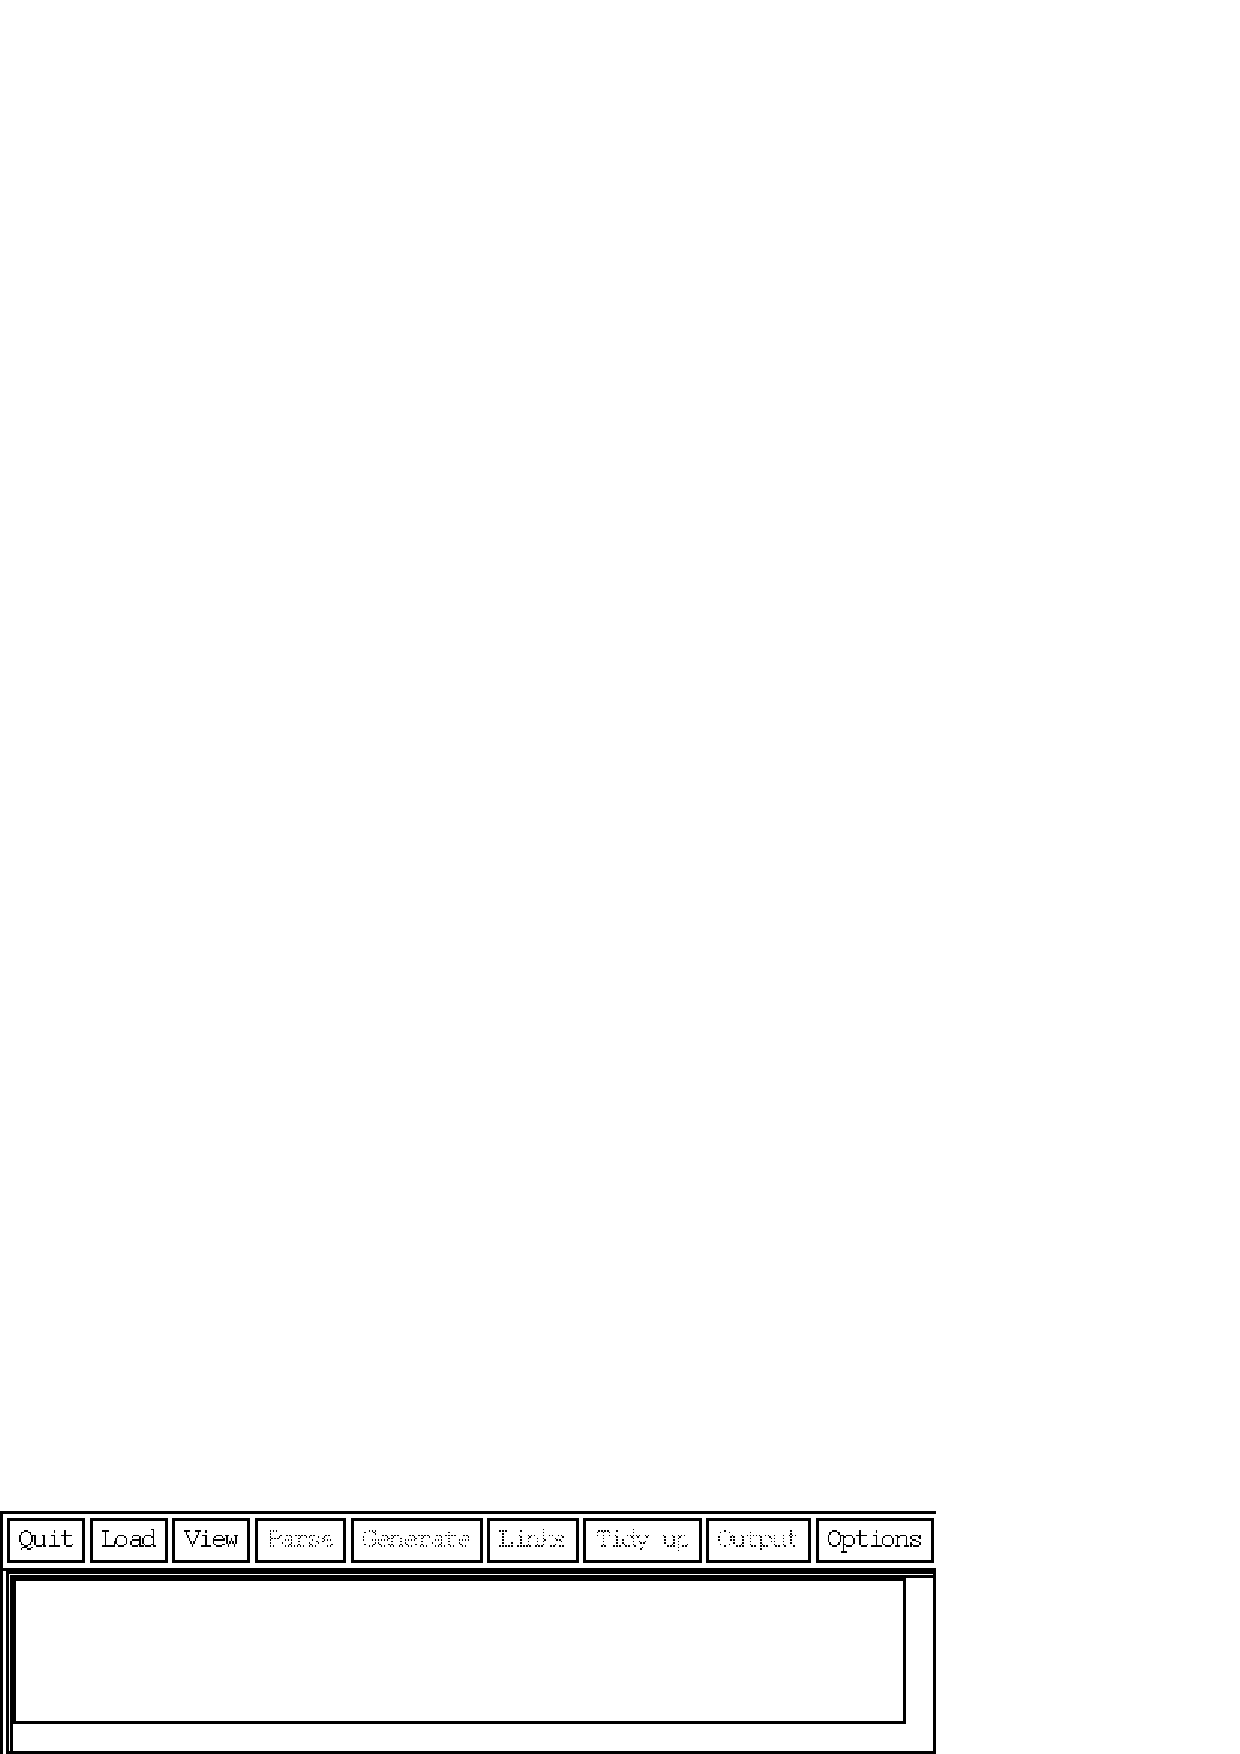
\includegraphics[width=400bp]{figs/lkbtop-unix}
\end{center}
\caption{The LKB interaction window in ACL/CLIM}
\label{lunix2}
\end{figure}
The main difference between the Mac and ACL/CLIM versions of the
LKB is the appearance of the top-level interaction menu.
The Mac version makes use of the Mac main menu-bar, and adds an LKB
menu to that.  LKB error messages etc appear in the MCL
Listener window.  For the ACL/CLIM version, there is a distinct
top level interaction window, with the menu displayed using
buttons across the top of the window.  From now on,
we will ignore these differences.
We will use the term `LKB top menu' 
for the menu and `LKB interaction window' for the window in which messages 
appear
for both the Mac and CLIM versions.  The illustrations in 
the rest of this
document show the CLIM interface.

Note that, in the ACL version, it is possible (though 
a little difficult) for the interaction
window to be closed inadvertently.
It may be reopened by evaluating
(clim-user::restart-lkb-window) in Lisp (i.e., the
{\tt *common-lisp*} buffer in emacs).
In both versions it is possible to end up in a state 
where most of the commands are unavailable because the system
does not think a grammar has been loaded: to
fix this, evaluate (enable-type-interactions).

\section{Loading a grammar}
\label{gramload}

The first step in this guided tour is to load an existing grammar: i.e.,
a set of files containing types and constraints, 
lexical entries, grammar rules etc.  
The LKB comes supplied with a series of grammars,
all of which are in the directory \filename{data}.  
There is a directory \filename{esslli}, which contains a series
of grammars of increasing complexity.
In this section, we
will assume that you are working with the smallest, which is called
`toy'.  

Select {\lkbmenucommand Complete grammar} from the LKB {\lkbmenucommand Load}
menu, and choose the file \filename{script} from the \filename{toy} directory
as shown in Figure~\ref{loadscript} for ACL/CLIM, MCL uses a standard
Mac file choice menu.
The script file is responsible for
loading the remainder of the files into the system.  You should see various
messages appearing in the interaction window, as shown in
Figure~\ref{loadmess}
(the interaction window has been enlarged).  
If there are any errors in the grammar which the system
can detect at this point, error messages will be displayed in this window.
With the toy grammar, there should be no errors, unless there is a problem 
associated with the temporary directory (see \S\ref{tempdir}).
If
you get another error message when trying to load 
\filename{toy/script}, it is
possible you have selected another file instead of script --- try again.
\begin{figure}
%\epsfxsize=3in
%\epsfbox[0 0 400 500]{figs/loadscript.ps}
\begin{center}
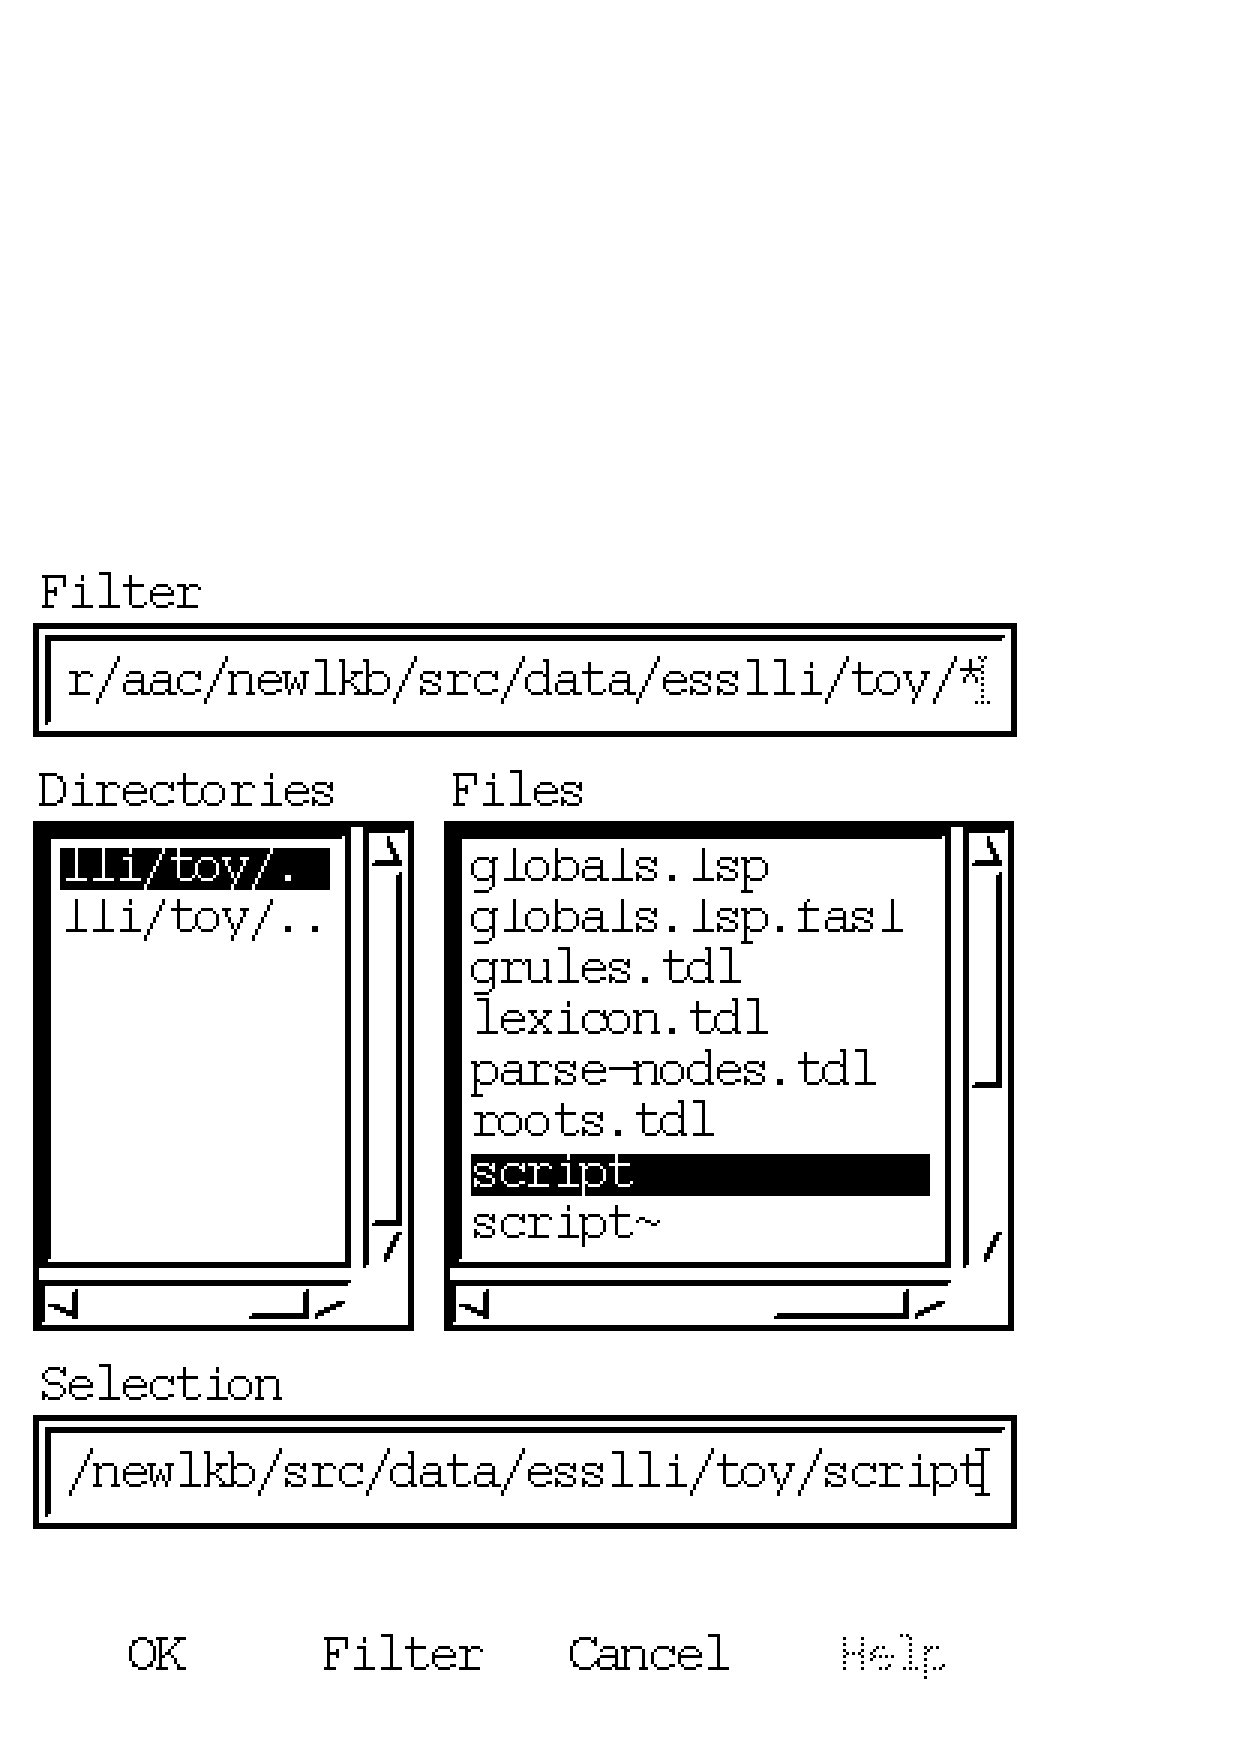
\includegraphics[width=3in]{figs/loadscript}
\end{center}
\caption{Selecting the script file in ACL/CLIM}
\label{loadscript}
\end{figure}
\begin{figure}
%\epsfbox[0 0 400 250]{figs/loadmess.ps}
\begin{center}
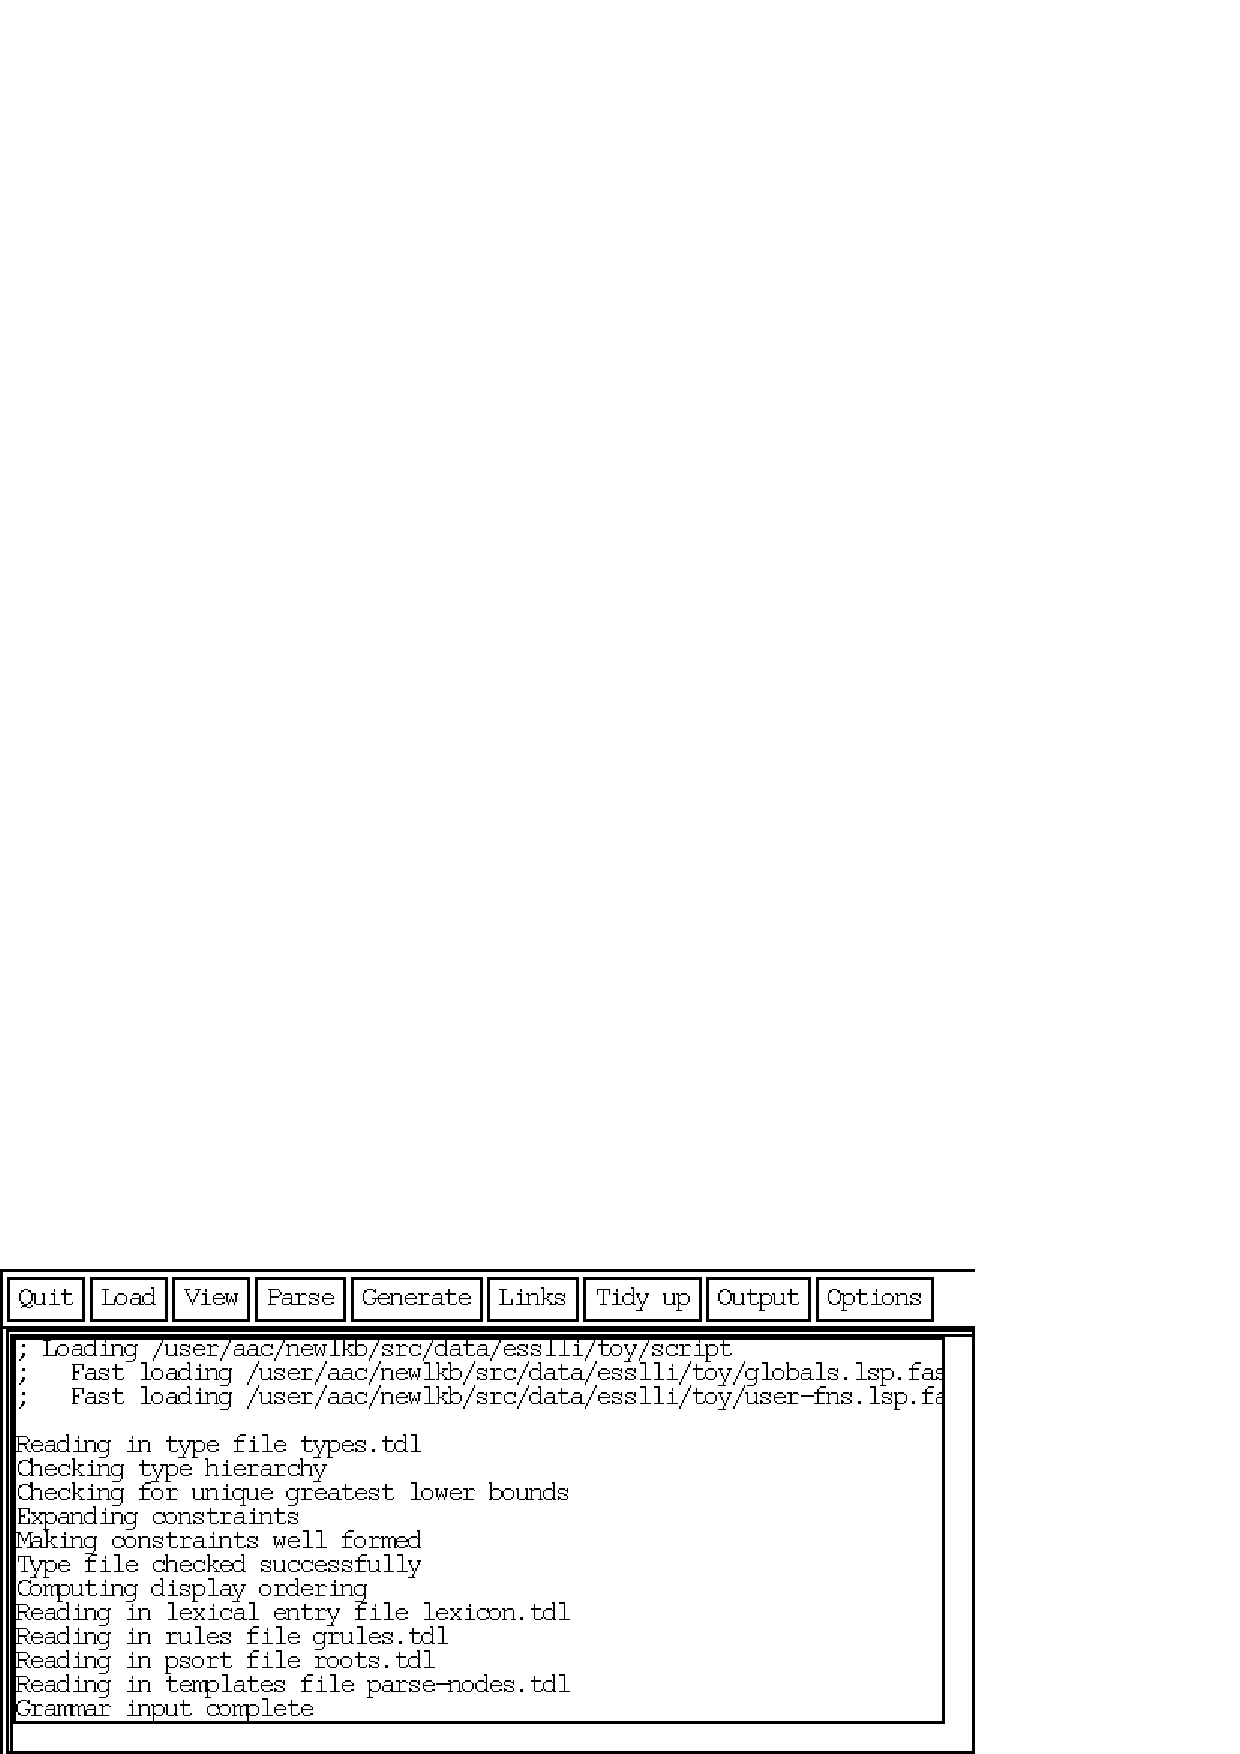
\includegraphics[width=3in]{figs/loadmess}
\end{center}
\caption{Loading a file}
\label{loadmess}
\end{figure}

Once a file is successfully loaded, the menu commands are all available
and a type hierarchy window is displayed (as shown in Figure~\ref{typehier}).
\begin{figure}
%\epsfxsize=3in
%\epsfbox[0 0 400 500]{figs/typehier.ps}
\begin{center}
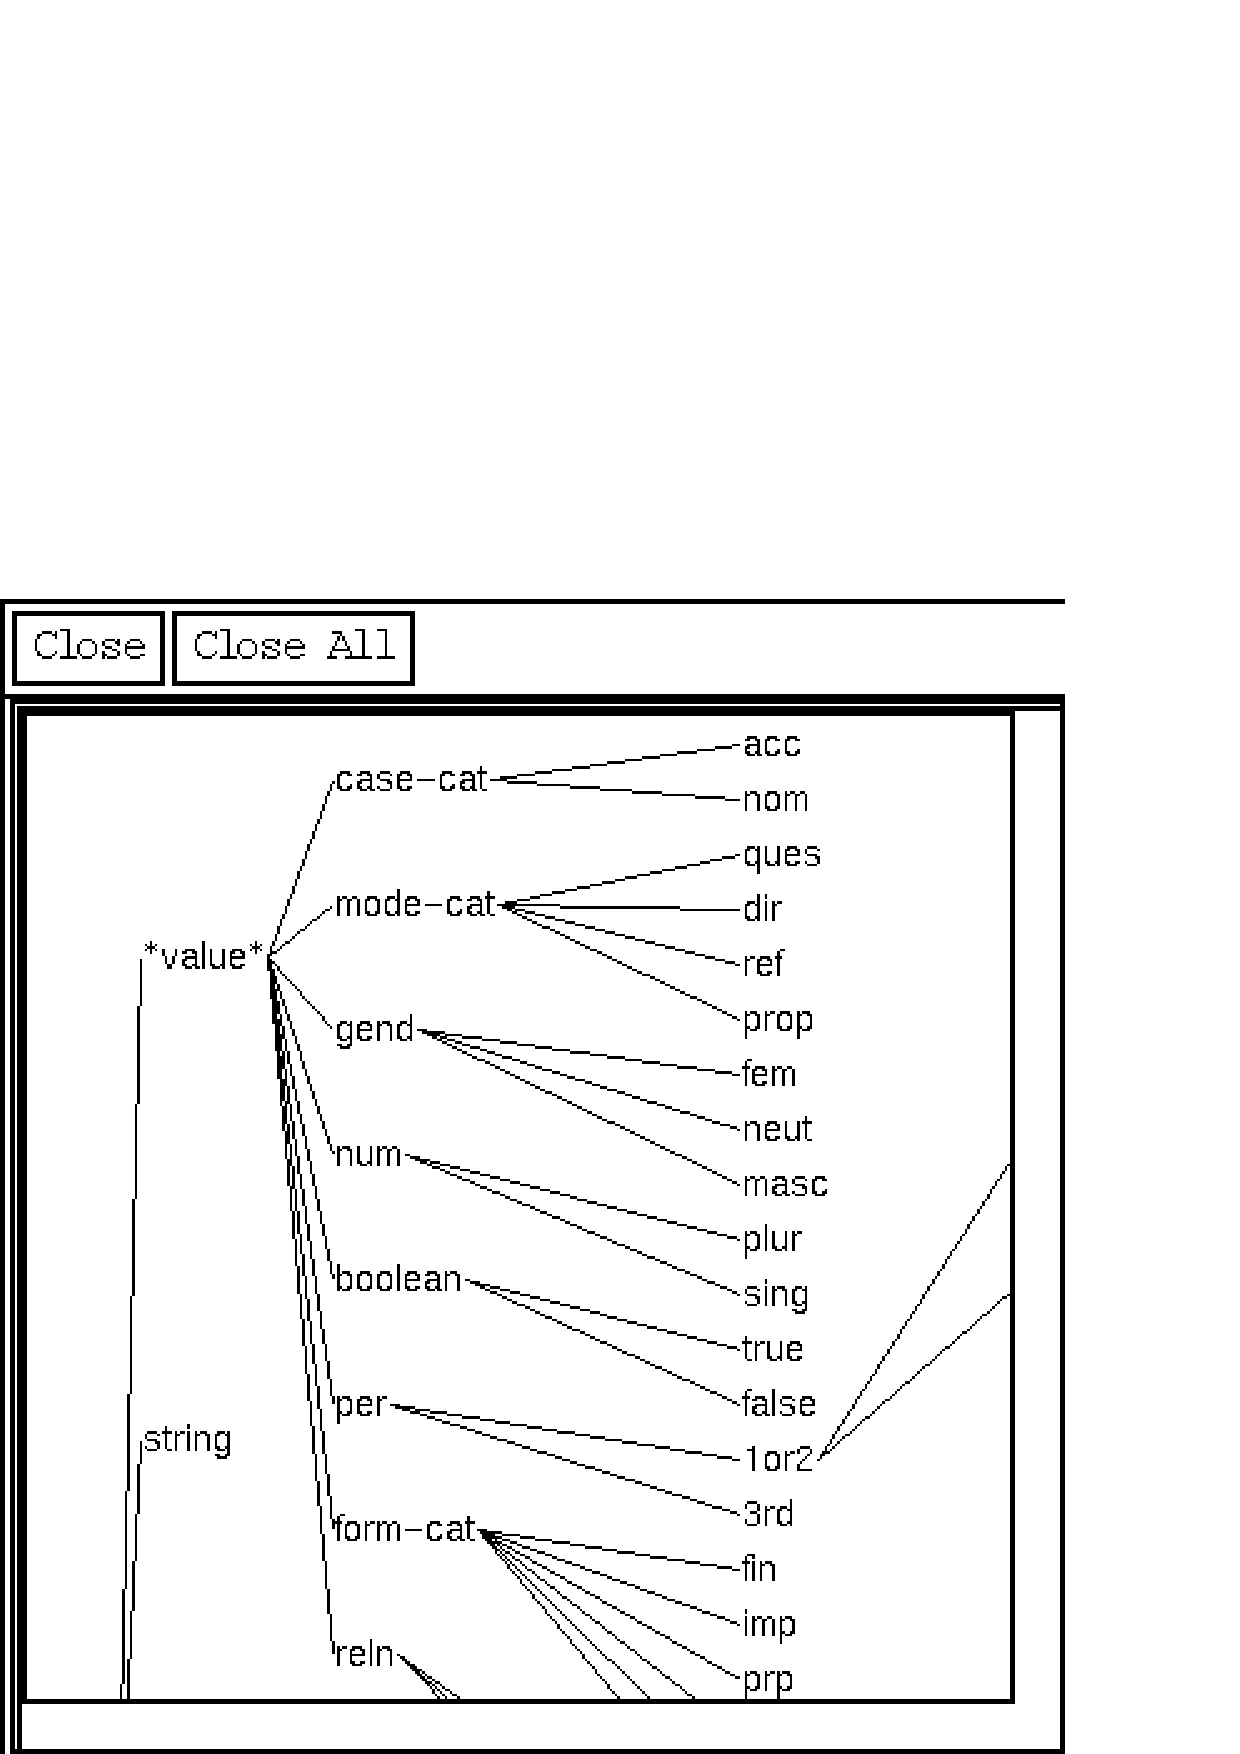
\includegraphics[width=3in]{figs/typehier}
\end{center}
\caption{The type hierarchy window}
\label{typehier}
\end{figure}


\section{Examining feature structures and type constraints}

In this section we will go through some of the ways in which
you can look at the data structures in the grammar, such as the types,
type constraints,
lexical entries and grammar rules.

\subsection{The type hierarchy window}
The backbone of any grammar in the LKB is the type system,
which consists of a hierarchy of types, each of which has a
constraint which is expressed as a feature structure.
The type hierarchy allows for inheritance of constraints.
In the LKB system, the type hierarchy window is shown 
with the most
general type displayed at the left of the window.  In the toy grammar, 
this is {\type *top*}.  
You will notice that there is some multiple inheritance in the hierarchy
(i.e., some types have more than one parent).

Click on the type {\type ne-list}
which is a daughter of {\type *list*}, which is a daughter of {\type *top*},
and choose {\lkbmenucommand Expanded Type} from the menu.  A window will appear
as shown in Figure~\ref{ne-list}.
\begin{figure}
%\epsfxsize=1in
%\epsfbox[0 0 200 200]{figs/ne-list.ps}
\begin{center}
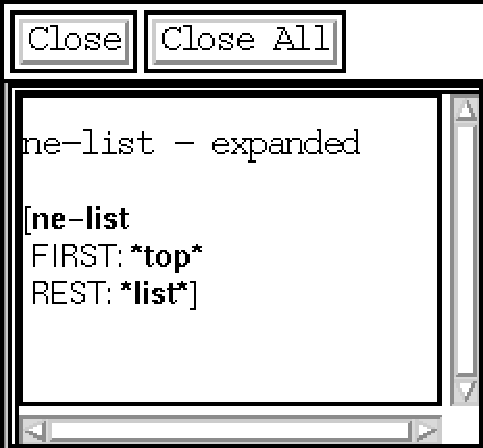
\includegraphics[width=2in]{figs/ne-list}
\caption{An expanded type constraint window}
\end{center}
\label{ne-list}
\end{figure}
This window shows the constraint on type {\type ne-list}: it has
two features, {\feature first} and {\feature rest}.  The value of
{\feature first} is {\type *top*}, which indicates it can unify with any
feature structure.  The value of {\feature rest} is {\type *list*}
which indicates it can only unify with something which is
of type {\type *list*} or one of its subtypes.  {\type *list*} and 
its daughters are important because they are used to implement
list structures which are found in several places in the grammar.

Look at the entry for the type {\type ne-list} in the actual source
file \filename{toy/types.tdl} (i.e., open that file in emacs, if you are
running the ACL/CLIM version of the LKB, or in the MCL editor, if you are
running the MCL version).
\begin{verbatim}
ne-list := *list* &
 [ FIRST *top*,
   REST *list* ].
\end{verbatim}
The syntax of the language in which the type and its constraint
are defined (the
\newterm{description language}) is detailed in \S\ref{typesyntax}.
The type definition obligatorily
specifies the parent or parents of a type (in this case,
{\type *list*}) and optionally gives a constraint definition.
In this particular case, the constraint described in the file corresponds
very closely to the expanded constraint shown in the
feature structure window, because the only parent of {\type ne-list} is
{\type *list*} and this does not have any features in its constraint.
However, in general, type constraints inherit a lot of information from
the ancestors of the type so the description of a constraint is very compact
compared to the expanded constraint.

To see a more complicated type constraint, 
click on {\type grule} (grammar rule)
in the type hierarchy 
window (found via {\type feat-struc}, 
{\type synsem-struc}, {\type phrase}
from {\type *top*})
and again choose {\lkbmenucommand Expanded Type}.
The feature structure window is shown in
Figure~\ref{grule}.  {\type grule} illustrates that types can have
complex constraints: that is the value of a feature in a constraint
can be a feature structure.  
\begin{figure}
%\epsfxsize=1in
%\epsfbox[0 0 200 400]{figs/grule.ps}
\begin{center}
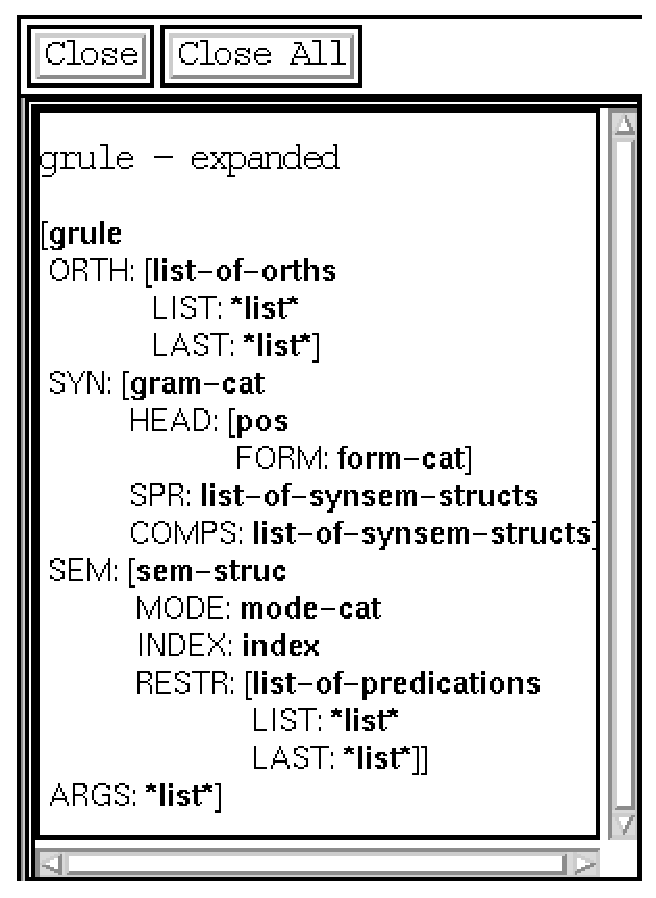
\includegraphics[width=3in]{figs/grule}
\end{center}
\caption{A complex type constraint}
\label{grule}
\end{figure}
Look at the definition of {\type grule} in the source file:
\begin{verbatim}
grule := phrase &
 [ ARGS *list* ].
\end{verbatim}
In contrast to {\type ne-list}, the constraint on
{\type grule} has inherited a lot of
information from types higher in the
hierarchy: you can see how this inheritance
operates by looking at the constraints of {\type grule}'s ancestors in the
type hierarchy window.

You will find that
you can click on the types within the feature structures to get menus
and also on the description at the top of the window
(e.g., {\tt grule - expanded}).
Details of the menu options in feature structure windows 
are given in \S\ref{activefs}.
More details of the type hierarchy window, including an explanation of all the
commands,
are given in \S\ref{thier}.

\subsection{The View commands}

The view commands let you get at entities such as lexical entries which cannot
be accessed from the type hierarchy window.  

Select {\lkbmenucommand View} from the LKB top menu and then select 
{\lkbmenucommand Word entries}.
You will be prompted for a word which corresponds to a lexical entry.
Enter {\tt kim} (case doesn't matter), deleting the default that
is specified (unless of course the default is {\tt KIM}, in which
case just select {\tt OK}).
You should get a feature structure window corresponding to the entry 
which has orthography ``kim'' in the toy grammar.
If there were multiple entries with the spelling `kim' they would all
be displayed. 

You can also access lexical entries by entering an identifier: to
do this you select {\lkbmenucommand View} {\lkbmenucommand Lex Entry}.  
To try this out, try entering {\tt kim\_1}.
An identifier will always
give a unique lexical entry.  

You might like 
to compare the feature structures shown with the actual lexical
entries in the file toy/lexicon.tdl, to see how the inheritance from type
constraints operates.  For instance, the actual entry for {\it Kim} is
simply:
\begin{verbatim}
kim_1 := pn-lxm & 
 [ ORTH <! "kim" !>,
   SEM [ RESTR <! [ NAME 'Kim ] !> ] ].
\end{verbatim}

Now try {\lkbmenucommand View} {\lkbmenucommand Grammar rule} and 
enter the identifier
{\tt head-specifier-rule} (or choose
it from the selections if a 
menu is displayed).  You will see the the grammar rule
is also a typed feature structure as shown in Figure~\ref{rulefs}.
We do not reproduce it in full here, because
it will not fit on one page, but the boxes indicate which parts of the
structure have been `shrunk' (this is done by clicking on a node,
and choosing the menu option {\lkbmenucommand Shrink/expand}).
\begin{figure}
%\epsfxsize=4in
%\epsfbox[0 0 400 800]{figs/rulefs.ps}
\begin{center}
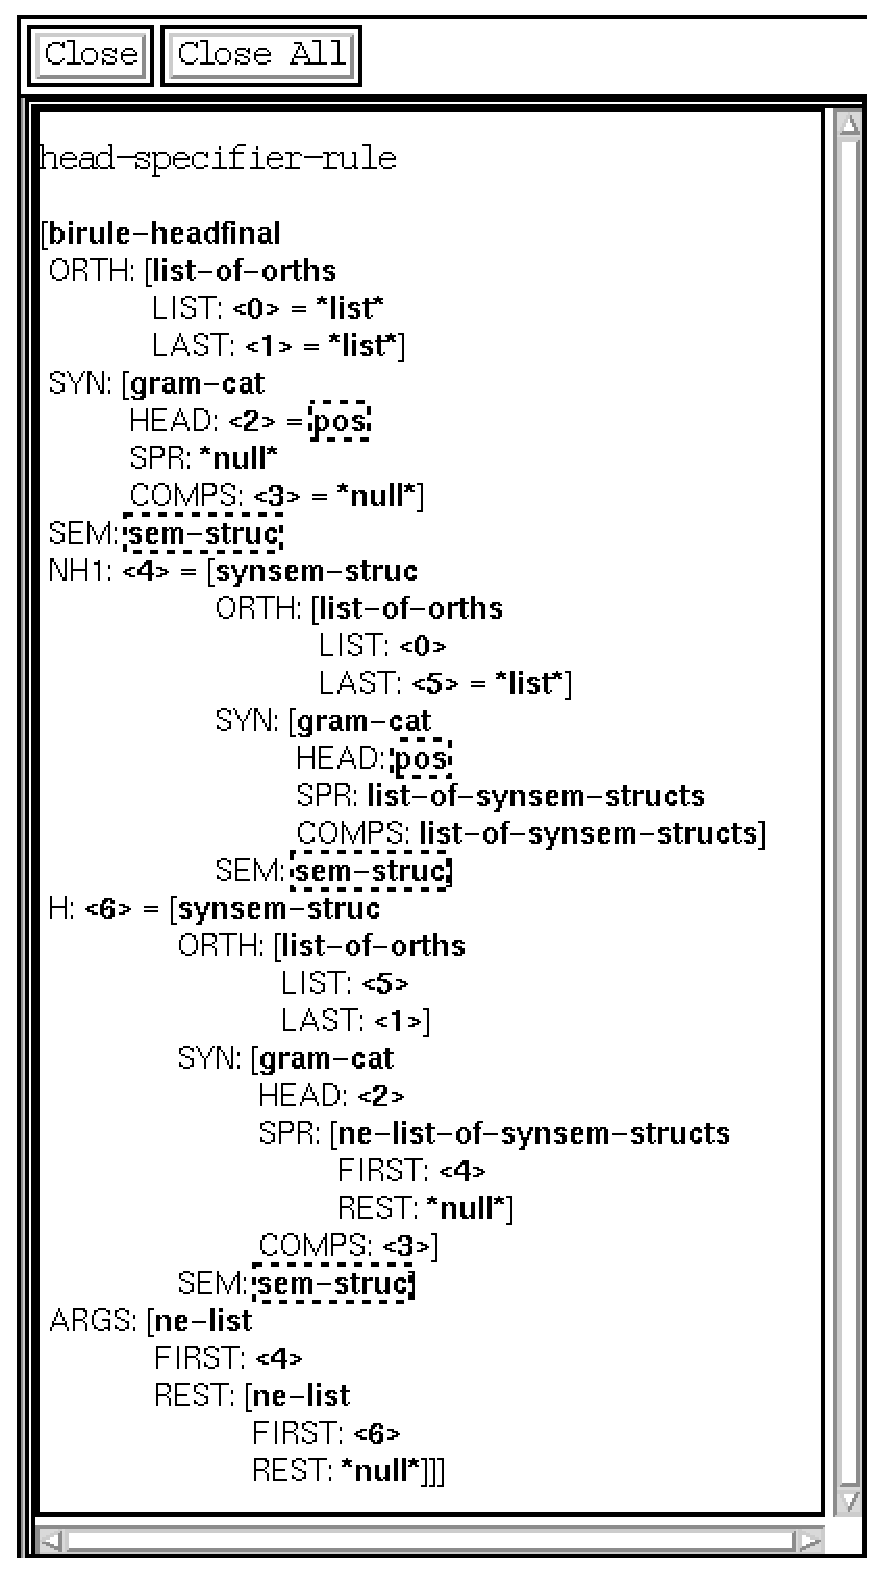
\includegraphics[height=4in]{figs/rulefs}
\end{center}
\caption{The head specifier rule}
\label{rulefs}
\end{figure}
A feature structure that encodes a rule can be thought of
as consisting of a number of `slots', into which the phrases for
the daughters and the mother fit.  To see how this works,
we will next describe how to parse a sentence.

\section{Parsing}

To parse a sentence, click on {\lkbmenucommand Parse} / {\lkbmenucommand Parse input}.  
Unless you have been parsing other things already,
the default selection is {\tt Kim sleeps}.  Click {\tt OK} to
accept this default.  In ACL/CLIM
you will get a window with one tiny parse
tree, as shown in Figure~\ref{kimsleeps}.\footnote{The reason for the
small size is that with non-trivial grammars and sentences, the parse 
trees can be very large and numerous \ldots} If you click on the parse
tree itself you will get a menu with an option to {\lkbmenucommand Show enlarged tree}.
If you choose this, you will see a window with a more readable version
of the tree, as shown in Figure~\ref{ptree}. In MCL you will just get the 
large tree immediately.
\begin{figure}
%\epsfxsize=2in
%\epsfbox[0 0 400 100]{figs/kimsleeps.ps}
\begin{center}
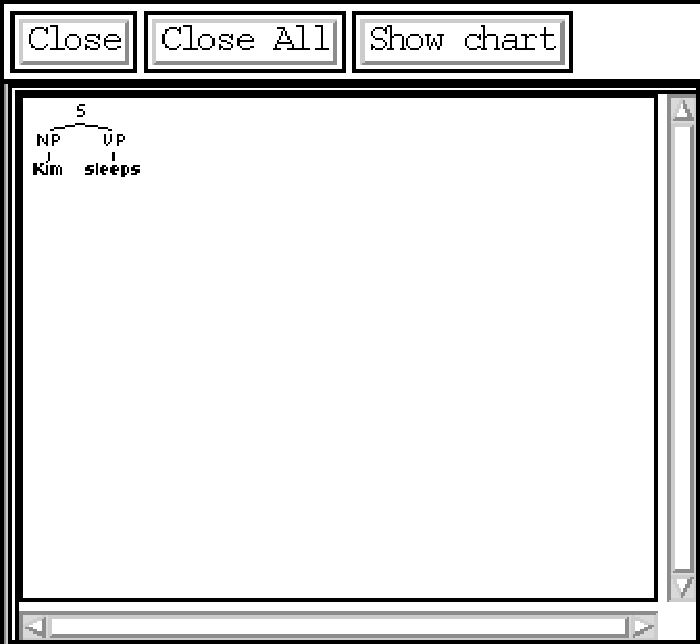
\includegraphics[width=3in]{figs/kimsleeps}
\end{center}
\caption{The parse result window in ACL/CLIM}
\label{kimsleeps}
\end{figure}
\begin{figure}
%\epsfxsize=2in
%\epsfbox[0 0 400 400]{figs/ptree.ps}
\begin{center}
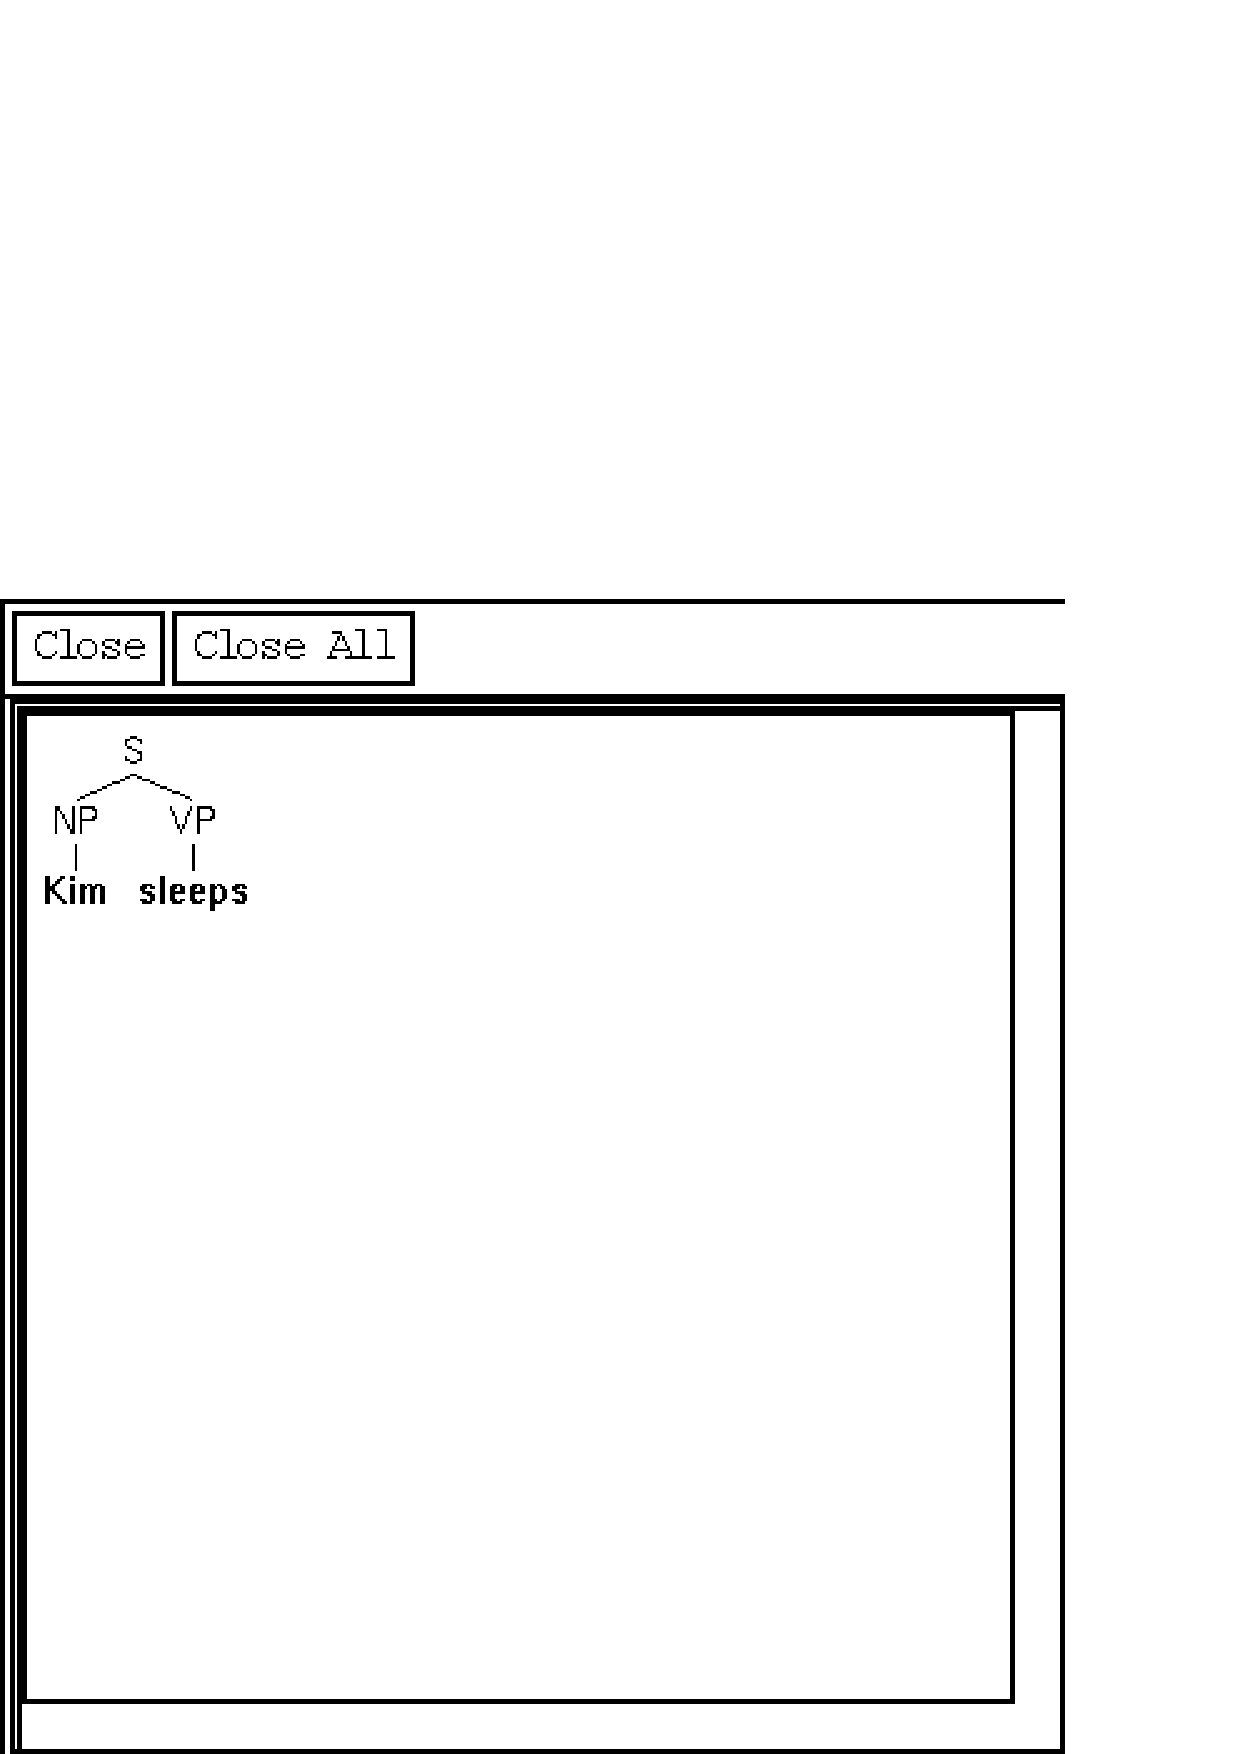
\includegraphics[width=3in]{figs/ptree}
\end{center}
\caption{A parse tree window}
\label{ptree}
\end{figure}

In a linguistic framework such as HPSG, a parse tree is just a convenient
user interface device, which is shorthand for a much larger typed
feature structure.  Click on the uppermost (S) node of the
enlarged parse tree and choose the option 
{\lkbmenucommand Feature structure --- Edge 3}.  
You will
see a large feature structure, which is shown in Figure~\ref{bigfs}.
As before, we have `shrunk' some parts of the structure so that
it can be displayed on the page.
This structure represents the entire
sentence.  It is an instantiation of the \lkbentryname{head-specifier-rule}
shown in Figure~\ref{rulefs}.
\begin{figure}
%\epsfxsize=4in
%\epsfbox[0 0 400 800]{figs/bigfs.ps}
\begin{center}
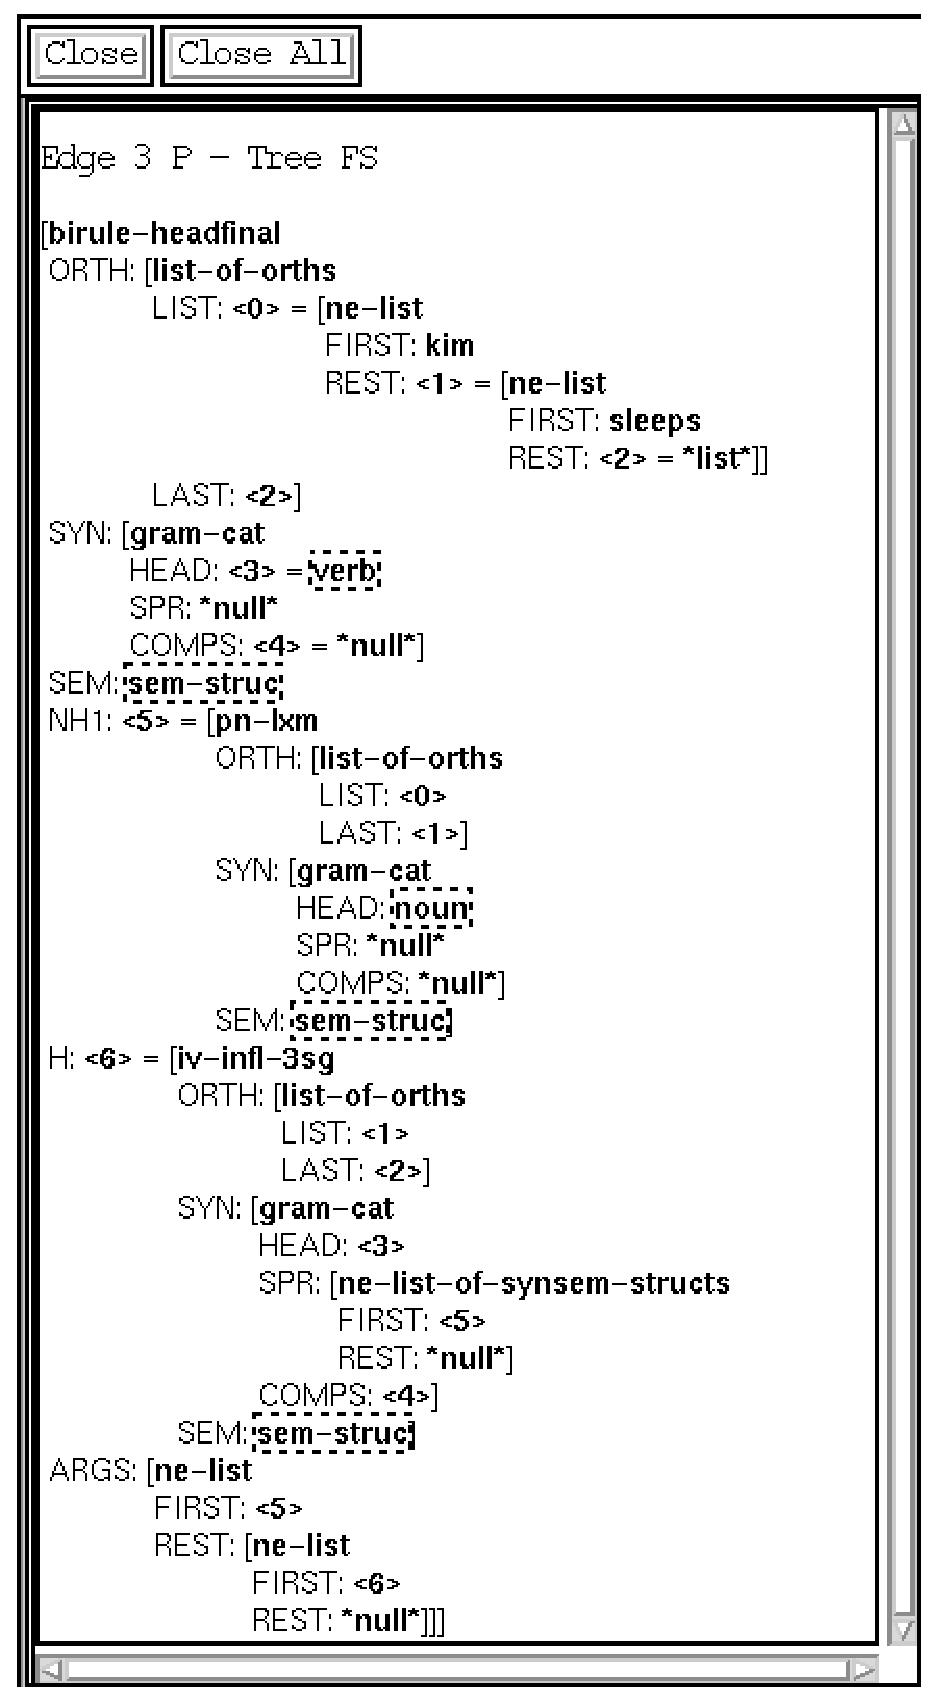
\includegraphics[height=4in]{figs/bigfs}
\end{center}
\caption{A feature structure representing the sentence {\it Kim sleeps}}
\label{bigfs}
\end{figure}

Note that the mother node in the parse tree corresponds
to the root node of the feature structure shown in Figure~\ref{bigfs}.
The structure for the word {\it Kim} is the node which
is the value of the feature {\feature nh1}.  The structure for the
verb {\it sleeps} is the value of {\feature h}.
The parse trees are created from the feature structures
by matching these substructures against a set of node specifiers
defined in the file \filename{parse-nodes.tdl}.
If you now try parsing the sentence {\it Kim likes Sandy}
and examining the trees and the feature structures as before, you
will see that the daughter structures may themselves have daughters.
We will go into a lot more detail about how grammar rules work
in the next chapter.

Now try {\lkbmenucommand Parse} / {\lkbmenucommand Batch Parse}.  
You will be prompted for the
name of a file which contains a test suite: i.e. a list of sentences
which either should or should not parse in a grammar.  A suitable file,
\filename{test.items}, already exists in the toy directory.  Select 
\filename{test.items} and enter the name of a new file for the output,
e.g., \filename{test.items.out}.  When you open the output file in
the editor, it should show the following for each sentence:
\begin{enumerate}
\item the number of the sentence
\item the sentence itself delimited by {\tt "}
\item the number of parses (0 if there were no parses)
\item the number of edges (roughly speaking an edge is a
phrase constructed while attempting to parse) 
\end{enumerate}
Note that we have marked ungrammatical sentences with an asterisk
in the test suite file, and though the parser strips off the asterisk before 
attempting to parse, the results file shows the sentence in the
form in which it was input. 
The results file also contains a time for the total processing.

The toy grammar can parse exactly four 
sentences.  In the next sections, we'll expand that coverage slightly.


\section{Adding a lexical entry}

In this section and the next one, we illustrate the basics of how you can
modify an existing grammar.
In this section, we describe how to add a new lexical entry.\footnote{You 
may want to make a backup copy of the toy
directory at this point before you start editing the files.}
First open the file \filename{toy/lexicon.tdl} in your text 
editor.
You will see that
the toy grammar has four lexical entries: two proper names and two verbs.
Suppose you want to add another proper name,
perhaps your own first name.  The entry will look exactly like
the entry for {\it Kim}, but with the orthography and value
of the semantic feature {\feature name} replaced with your name.\footnote{If your name
has spaces in it, please write it without a space for now.  
The LKB can deal with words with spaces in them, see \S\ref{multiword},
but discussing this would take us too far afield at the moment.  If your name contains
diacritical marks etc, like \'{e}, then you can enter these 
using the normal Macintosh sequences 
in the MCL text editor.  For emacs, {\tt M-x iso-accents-mode} allows
you to enter accented characters.  
However, there are some problems --- see \S\ref{accents} for a more
detailed discussion.}
Add such an entry to the end of the file.
For instance:
\begin{verbatim}
ann_1 := pn-lxm & 
 [ ORTH <! "ann" !>,
   SEM [ RESTR <! [ NAME 'ann ] !> ] ].
\end{verbatim}

Save the file, and then select {\lkbmenucommand Load}
followed by {\lkbmenucommand Reload grammar}.  This will reload the script file that
you loaded before, this time loading the changed version of the lexicon.
You may get some error messages in the LKB interaction window
at this point, if you have left
out a character, for example.  If you cannot see what is wrong, the
description of the error messages in \S\ref{synwf} may help you
track it down.  When you have successfully reloaded the system,
you should be able to parse some additional sentences, such as:
\begin{verbatim}
Ann sleeps
\end{verbatim}
If you find that a sentence won't parse, and you do not understand
why a grammar rule is not applying to a particular lexical
item, there are some tools to help you.  In particular,
\S\ref{unifcheck} describes an interactive tool for 
showing why unification is failing.

Once you have successfully parsed some new sentences,
you could add them to the list of test sentences for batch parsing.

\section{Adding a type and its constraint description}

The way the toy grammar is set up, although you could add a lexical
entry for a proper name by just adding a description to the lexicon file,
in order to add a new verb to the lexicon, you have to first add a type
representing its relation.  Suppose you want to add a new entry for
the intransitive verb {\it snores}.  First you have to add a type such as
{\type snore\_rel}.  Open the file \filename{toy/types.tdl}.  Search the file for
the entry for the relation for sleeps, {\type r\_sleep}.  Then add a new
entry for {\type r\_snore}.  You can then save the file, and add a new entry
to the lexicon file.  As with the previous entry, you can basically do
this by copying the existing entry for {\it sleeps},
but this time you have to 
change the relation to be the type you have just added.
Change the orthography and the identifier for the entry as before.
Save the file.  Then select {\lkbmenucommand Reload grammar}.  As before, check
the LKB interaction window to make sure reloading was successful 
and try parsing
some new sentences.


\section{Next steps}

If you have worked through this chapter, and are a beginner to the use of typed
feature structure systems, we have now to admit that we've led you gently to
the edge of a small but steep cliff and are not going to provide much in the
way of climbing equipment.\footnote{There is the possibility of Copestake and
Flickinger (next millennium), which would be an introduction to linguistic
engineering using typed feature structure systems, and the LKB in particular.
% UPDATE pount - millennium ...
If you think this would be a worthwhile enterprise, please send encouraging
email, cash donations etc to us at CSLI.}  
A basic introduction to the notion of typed feature structure
grammars, avoiding formal notation,
is in the next chapter (Chapter~\ref{easy}).
Alternatively, the 
formal exposition of types and typed feature structures as used in the LKB
is in Chapter~\ref{formal}.  
Chapter~\ref{formal} is designed for readers who have some familiarity
with feature structures and are happy with a fairly technical exposition.  
Many people will be happier investigating the properties of the
system informally first and then checking Chapter~\ref{formal} 
to understand the precise behaviour.  With
the exception of those chapters, the rest of this document is intended as a
reference manual.  

Ideally, once you understand the basics of the formalism to the level presented
in Chapter~\ref{easy}, you would investigate the capabilities of the LKB
further by working through some of the details of the example grammars, and try
extending them, first by adding lexical entries as we did in this chapter, and
then by extending the coverage by adding new lexical types.  You should refer
to the relevant sections in chapters~\ref{formal}, \ref{srcfiles} and \ref{ui}
when problems arise or when you need to know the details of some facility.
Then \S\ref{own} gives some hints as to how to go about building your own
grammar.  Some of the advanced capabilities discussed in Chapter~\ref{advanced}
will become relevant at this point.

If you want to learn more about a linguistic framework that uses the typed
feature structure formalism, then Sag and Wasow (1999) is an introductory
textbook.  Some of the grammars provided with the LKB system implement the
grammars described there.  Sag and Wasow use a somewhat different (and much
less tractable) formalism from the version of the typed feature structure logic
used in the LKB system and their terminology also differs.  Most importantly,
they use the term \newterm{typed feature structure description} where we talk
about typed feature structures.  However, Sag and Wasow make only limited
use of the extra power of the formalism they describe, so most of the grammars
they discuss can be encoded in the LKB.

\chapter{Typed feature structures made simple}
\label{easy}

If you have worked through the previous chapter, you should have
gained an intuitive idea of the components of a typed feature structure
grammar, how to write feature structure descriptions for lexical entries
etc, and how grammar rules work.  In this chapter we will go over the
underlying concepts in more detail, to give you a more precise (though 
still relatively informal)
description of typed feature structures.
This chapter could be read without access to a running
LKB system, although having the system available will be necessary to
work with the sample grammars and to do some of the exercises.  
If you have some familiarity
with typed feature structure formalisms, you should
read Chapter~\ref{formal} instead of this one.  In the case
of any apparent conflict between this chapter and Chapter~\ref{formal},
Chapter~\ref{formal} should be taken as definitive.  
However the description in this chapter is precise.  It roughly follows
the definitions in Chapter~\ref{formal} --- here, however,
we have used many more examples and far fewer mathematical symbols
(\newterm{squiggly bits}).

\paragraph{Cautionary note}  
There are several slightly different variants of
typed feature structure formalisms.  Here we are describing the 
version used in the LKB system, and since this is an informal
introduction, we will not discuss the differences with other approaches
in this chapter.  
Some of these differences are mentioned in Chapter~\ref{formal},
which gives more formal definitions.  We also omit references to
previous work --- again, see Chapter~\ref{formal}.
The terminology in the literature is also confusing, to say the least.  
Rather than trying to explain all the alternatives in the main
text, we have just given the terminology used elsewhere in this
documentation, with a couple of comments about the differences from
Sag and Wasow (1999), since this is probably the most likely
source of possible confusion.
%UPDATE
(Note, eventually we will produce a glossary which will make the 
relationships between the terminology clearer.
This chapter is a first draft: comments are very welcome, especially
from members of the target audience.)

Some sections in this chpater are followed by
exercises.  It's important to attempt at least
those which aren't marked as 
optional.  They shouldn't take more than a few minutes 
and sometimes we will use them to introduce new material.

Before we start describing the details of the formalism,
we are going to introduce a really tiny grammar, both in order
to make the concept of encoding a grammar in feature structures clearer,
and also to give us concrete examples that can be used in the discussion
of the typed feature structures themselves.  


\section{A really really simple grammar}

We expect that readers have some familiarity with
grammars defined in terms of atomic symbols.  For instance,
Figure~\ref{smplatomic} shows a very simple grammar and lexicon,
with just two grammar rules and six lexical entries.
\begin{figure}
\begin{center}
{\small
\begin{minipage}[t]{3in}
\begin{verbatim}
Start symbol: S

Rules:

S -> NP VP
NP -> Det N
\end{verbatim}
\end{minipage}
\begin{minipage}[t]{3in}
\begin{verbatim}
Lexicon:

dog : N
dogs: N
this : Det
these: Det
sleeps : VP
sleep: VP

\end{verbatim}
\end{minipage}}
\end{center}
\caption{A tiny grammar encoded using atomic symbols}
\label{smplatomic}
\end{figure}
The specification of the \newterm{start symbol} 
as {\tt S} means that the grammar will
accept as complete strings ``these dogs sleep'' and ``this dog sleeps'',
but not ``sleep'' and ``this dog'', because these cannot be assigned
the category S.

Grammars in general can be viewed abstractly as mappings between a 
set of descriptive structures and a set of
strings of characters.  
For a very simple grammar like
that in Figure~\ref{smplatomic}, 
we can use a labelled bracket notation as
the description.  For instance:
\begin{verbatim}
(S (NP (Det this) (N dog)) (VP sleeps))
\end{verbatim}
This labelled bracketing can equivalently 
be drawn as a tree, as shown in Figure~\ref{trivtree}.
\begin{figure}[!ht]
\begin{center}
\setlength{\unitlength}{0.5in}
\begin{picture}(3,3)(0,0.25)
\thicklines
\put(2,3){\makebox(0,0){\strut S}}
\put(1.9,2.9){\line(-1, -1){0.7}}
\put(2.1,2.9){\line(1, -1){0.7}}
%
\put(3,2){\makebox(0,0){\strut VP}}
%
\put(1,2){\makebox(0,0){\strut NP}}
\put(0.9,1.9){\line(-1, -1){0.7}}
\put(1.1,1.9){\line(1, -1){0.7}}
%
\put(0,1){\makebox(0,0){\strut Det}}
\put(2,1){\makebox(0,0){\strut N}}
%
\put(0,0.5){\makebox(0,0){\strut this}}
\put(2,0.5){\makebox(0,0){\strut dog}}
\put(3,0.5){\makebox(0,0){\strut sleeps}}
\end{picture}
\end{center}
\caption{Tree for {\it this dog sleeps} with the 
tiny grammar using atomic symbols}
\label{trivtree}
\end{figure}

Grammars can also be viewed as specifications that allow
parsing and generation of strings given partial information.
For instance, given the input string:
\begin{verbatim}
these dogs sleep
\end{verbatim}
we could derive the single labelled bracketing:
\begin{verbatim}
(S (NP (Det these) (N dogs)) (VP sleep))
\end{verbatim}
Given the partial bracketed structure:
\begin{verbatim}
(S (NP (Det ?) (N ?)) (VP sleeps))
\end{verbatim}
(where we are just using {\tt ?}
as a placeholder) the corresponding strings are:
\begin{verbatim}
this dog sleeps
these dog sleeps
this dogs sleeps
these dogs sleeps
\end{verbatim}

As this example shows, this grammar allows
sentences which are not grammatical English, such as:
\begin{ex}
these dog sleeps
\end{ex}
The problem is that the grammar does not include any specification of
agreement.  It could be fixed by increasing the number of atomic symbols,
for instance as shown in Figure~\ref{agratomic}.
But this approach
would soon become very tedious as we expanded the grammar.
\begin{figure}[!ht]
{\small
\begin{minipage}[t]{3in}
\begin{verbatim}
Start symbol: S

Rules:

S -> NP-sg VP-sg
S -> NP-pl VP-pl
NP-sg -> Det-sg N-sg
NP-pl -> Det-pl N-pl

\end{verbatim}
\end{minipage}
\begin{minipage}[t]{3in}
\begin{verbatim}
Lexicon:

dog : N-sg
dogs: N-pl
this : Det-sg
these: Det-pl
sleeps : VP-sg
sleep: VP-pl
\end{verbatim}
\end{minipage}}
\caption{An atomic symbol grammar encoding subject verb agreement}
\label{agratomic}
\end{figure}

Feature structures are one way of allowing extra information
to be encoded to
deal with agreement and more complex phenomena.  
Some approaches to representation use such feature structures
to augment a backbone of rules expressed using atomic symbols.
However, in other approaches, including that implemented in the
LKB, we instead make everything be a 
(typed) feature structure, including lexical entries
and grammar rules.  

Figure~\ref{lkbgram1} shows how a grammar equivalent to the very
simple grammar shown above can be written using
typed feature structures.
%
\begin{figure}
{\small
\begin{minipage}[t]{3in}
\begin{verbatim}
;;; Types
string := *top*.

*list* := *top*.

*ne-list* := *list* &
 [ FIRST *top*,
   REST *list* ].

*null* := *list*.

synsem-struc := *top* &
[ CATEGORY cat ].

cat := *top*.

s := cat.

np := cat.

vp := cat.

det := cat.

n := cat.

phrase := synsem-struc &
[ ARGS *list* ].

lexeme := synsem-struc &
[ ORTH string ].

root := phrase &
[ CATEGORY s ].
\end{verbatim}
\end{minipage}
\begin{minipage}[t]{3in}
\begin{verbatim}
;;; Lexicon
this := lexeme &
[ ORTH "this",
  CATEGORY det ].

these := lexeme &
[ ORTH "these",
  CATEGORY det ].

sleep := lexeme &
[ ORTH "sleep",
  CATEGORY vp ].

sleeps := lexeme &
[ ORTH "sleeps",
  CATEGORY vp ].

dog := lexeme &
[ ORTH "dog",
  CATEGORY n ].

dogs := lexeme &
[ ORTH "dogs",
  CATEGORY n ].

;;; Rules
s_rule := phrase &
[ CATEGORY s,
  ARGS [ FIRST [ CATEGORY np ],
         REST [ FIRST [ CATEGORY vp ],
                REST *null* ]]] .

np_rule := phrase &
[ CATEGORY np,
  ARGS [ FIRST [ CATEGORY det ],
         REST [ FIRST [ CATEGORY n ],
                REST *null* ]]] .
\end{verbatim}
\end{minipage}
}
\caption{Tiny typed feature structure grammar}
\label{lkbgram1}
\end{figure}
%
This is the grammar that is in the directory 
\filename{tiniest/grammar1} distributed with the LKB.
You should load this grammar into the LKB system in order to
experiment.
Figure~\ref{lkbgram1} looks much more complex than the grammar given 
in Figure~\ref{smplatomic}, but 
the 
additional initial complexity of feature structure grammars pays off 
with more complex grammars.\footnote{In fact this grammar is a bit
more complex than it needed to be 
to simply simulate the starting grammar in the LKB system, but we've
done this in order to be consistent with 
some of the other grammars distributed 
with the LKB, such as the toy grammar discussed in the previous
chapter.  As we'll see in a lot of detail later on,
although the LKB system can process any grammar that
can be expressed in this variant of the typed feature structure 
formalism, there are a few parameters which control the interface 
between the grammar and the system which have to be declared.  
For simplicity, we've kept most of those parameters the same in
the sample grammars supplied with the system.}
Please note that this isn't intended to be in any way a linguistically
interesting grammar
(unlike the toy grammar used in the last
chapter, which does have theoretically motivated fundamentals,
but which is somewhat too complex to use for our current
purposes).  

We will not go through the operation
of the grammar here, but rely on the intuitive correspondence
with the grammar in Figure~\ref{smplatomic}.
The details will emerge as we discuss the
formalism.
For now, you should just note that 
the basic components of the grammar are:
\begin{description}
\item[The type system]  (left column of Figure~\ref{lkbgram1})\\
The type system acts as the defining
framework for the rest of the grammar.  For instance,
it determines which structures
are mutually compatible and which features can occur, and it sets
up an inheritance system which allows generalisations to be 
expressed.  For this particular grammar, for example,
all the basic linguistic entities
are of type {\type synsem-struc} which the type system defines
to have the feature {\feature category}.
The information which was conveyed by the simple atomic categories
in the grammar in Figure~\ref{smplatomic}
is kept in this feature.
The categories themselves, {\type s}, {\type np} and so
on, are also represented as types. 
All types must be explicitly defined, except for
string types such as {\tt "these"}.
\item[Lexical entries]  (top two-thirds of 
right column of Figure~\ref{lkbgram1})\\
These are typed feature structures
which the grammar writer constructs in order to encode the words
of the language.  Lexical entries define a relationship 
between a string representing the characters in a word
and some linguistic description of the word (or, more precisely,
of a particular sense of a word).
In this grammar,
the {\feature orth} (orthography)
feature is used to encode the string in lexical 
entries.  
\item[Grammar rules] (bottom third of 
right column of Figure~\ref{lkbgram1})\\
Grammar rules are typed feature structures that
describe how to combine lexical entries and phrases
to make further phrases.  In the atomic category grammar, we expressed 
the idea of a rule in a conventional way by specifying 
a category for a phrase
to the left of an arrow, and the daughter categories, in their
expected linear order, to the right of the arrow.
For this feature structure grammar
we have made the mother structure actually
include the daughters.\footnote{This isn't a requirement of the LKB system
but it's an approach used in most grammars in the HPSG framework.}  
Thus, the rules are actually partial descriptions
of phrases.  The daughters of the phrase are
contained in the feature {\feature args}.  This takes as its value a list
where the order of the list elements
corresponds
to the linear order of the daughters.  
Note that we will sometimes collectively refer to lexical entries
and grammar rules as \newterm{entries}.
\item[Start symbol]
The equivalent of the
start symbol in the atomic category grammar
is represented by the type {\type root}.
\end{description}

For this grammar, we could still derive the same labelled
bracketing for {\it this dog sleeps} as we saw before,
by simply taking the values of the category feature
from the lexical entries and from each phrase.
But with a feature structure grammar, a tree with atomic
labels is just an abbreviation for 
the complete representation.
For this style of grammar, where the mother of a rule
is reprsented as a feature structure that contains all its daughters,
the complete representation
for the derivation is
given by the feature structure for the sentence.
This structure
is shown in Figure~\ref{phraseavm}.  
\begin{figure}
\begin{center}
{\tiny
$\avmplus{\att{phrase}\\
\attvaltyp{CATEGORY}{s}\\
\attval{ARGS}{\avmplus{\att{*ne-list*}\\
\attval{FIRST}{\avmplus{\att{phrase}\\
\attvaltyp{CATEGORY}{np}\\
\attval{ARGS}{\avmplus{\att{*ne-list*}\\
\attval{FIRST}{\avmplus{\att{lexeme}\\                                                
\attvaltyp{ORTH}{"this"}\\                                                      
\attvaltyp{CATEGORY}{det}}}\\                            
\attval{REST}{\avmplus{\att{*ne-list*}\\                                                   
\attval{FIRST}{\avmplus{\att{lexeme}\\
\attvaltyp{ORTH}{"dog"}\\   
\attvaltyp{CATEGORY}{n}}}\\
\attvaltyp{REST}{*null*}}}}}}}\\
\attval{REST}{\avmplus{\att{*ne-list*}\\                                                   
\attval{FIRST}{\avmplus{\att{lexeme}\\
\attvaltyp{ORTH}{"sleeps"}\\                                                      
\attvaltyp{CATEGORY}{vp}}}\\
\attvaltyp{REST}{*null*}}}}}}$}
\end{center}
\caption{AVM for {\it this dog sleeps} from
the tiny grammar using feature structures}
\label{phraseavm}
\end{figure}

In the next few sections, we will use examples from this grammar, and some
slightly more complex variants of it, in order to explain 
typed feature structures in detail.
We'll start
off this detailed explanation of typed feature structures
by discussing \newterm{type system}s,
which form the backbone of grammars. 
A type system consists of a \newterm{type hierarchy}, which
indicates specialisation and consistency
of types, plus a set of \newterm{constraint}s
on types which determined which typed feature structures are 
\newterm{well-formed}.
The next section describes the type hierarchy.

\section{The type hierarchy}
\label{easythier}

Figure~\ref{th}
shows the type hierarchy corresponding to our simple grammar
(with the string types omitted).
\begin{figure}[!ht]
\begin{center}
\setlength{\unitlength}{0.95in}
\begin{picture}(6.5,1.7)(0,2.4) 
\thicklines
\put(3,4){\makebox(0,0){\figtype{*top*}}}
\put(2.9,3.9){\line(-2, -1){0.6}}
\put(3.1,3.9){\line(2, -1){0.6}}
\put(2.2,3.5){\makebox(0,0){\figtype{string}}}
\put(3.8,3.5){\makebox(0,0){\figtype{synsem-struc}}}
\put(2.8,3.9){\line(-5, -1){1.6}}
\put(3.2,3.9){\line(5, -1){1.6}}
\put(1,3.5){\makebox(0,0){\figtype{*list*}}}
\put(5,3.5){\makebox(0,0){\figtype{cat}}}
%
\put(4.9,3.4){\line(-1, -1){0.3}}
\put(4.5,3.0){\makebox(0,0){\figtype{s}}}
\put(5.0,3.4){\line(0, -1){0.3}}
\put(5,3.0){\makebox(0,0){\figtype{vp}}}
\put(5.1,3.4){\line(1, -1){0.3}}
\put(5.5,3.0){\makebox(0,0){\figtype{np}}}
\put(5.15,3.4){\line(5, -2){0.8}}
\put(6.0,3.0){\makebox(0,0){\figtype{n}}}
\put(5.2,3.4){\line(4, -1){1.2}}
\put(6.5,3.0){\makebox(0,0){\figtype{det}}}
%
\put(0.9,3.4){\line(-2, -1){0.6}}
\put(1.1,3.4){\line(2, -1){0.6}}
\put(0.2,3.0){\makebox(0,0){\figtype{*ne-list*}}}
\put(1.8,3.0){\makebox(0,0){\figtype{*null*}}}
%
\put(3.8,3.4){\line(0, -1){0.3}}
\put(3.8,3.0){\makebox(0,0){\figtype{phrase}}}
\put(3.8,2.9){\line(0, -1){0.3}}
\put(3.8,2.5){\makebox(0,0){\figtype{root}}}
\put(3.7,3.4){\line(-2, -1){0.6}}
\put(3,3.0){\makebox(0,0){\figtype{lexeme}}}
\end{picture}
\end{center}
\caption{Type hierarchy for the tiny grammar}
\label{th}
\end{figure}
As in all type hierarchies, there is a
unique most general type, which we will refer to as the top type,
{\type *top*}.  
The way that
type files are written in the LKB
means that the
descriptions of types contain a specification of their parents together
with the constraint (see Figure~\ref{lkbgram1}, where, for instance,
{\type *ne-list*} is defined as having the parent {\type *list*}).
It is the specification of the parents that defines the type hierarchy.
Note that {\type *top*} is not
defined in the grammar specification.
The hierarchy determines how constraints are inherited,
although we won't get to the details until later in the chapter.
This particular hierarchy is a tree, it is possible
for a type to have more than one parent: this is usually
referred to as \newterm{multiple inheritance} and we'll see some examples
of it shortly.

Below is a short summary of 
the properties of type hierarchies in general.
(Later on, we'll give summaries of typed feature structures,
constraints and so on.)  All type hierarchies in the LKB system
must obey these conditions.

\paragraph{Properties of type hierarchies}
\begin{description}
\item[Unique top] There is a single hierarchy containing all the types
with a unique top type.
\item[No cycles] There are no cycles in the hierarchy.  
\item[Unique greatest lower bounds] 
Any two types in the hierarchy must either be incompatible,
in which case they will not share any descendants, or they must
have a unique highest common descendant (referred to as 
the unique \newterm{greatest lower bound}).
\end{description}

In order to make the last
restriction a bit clearer, we will use an artificial example of
a hierarchy (shown in Figure~\ref{th2}). 
\begin{figure}[!ht]
\begin{center}
\setlength{\unitlength}{1in}
\begin{picture}(6,3.2)(0.7,1.9) 
\thicklines
\put(3,4){\makebox(0,0){\figtype{*top*}}}
\put(3,3.9){\line(0, -1){0.3}}
\put(3,3.5){\makebox(0,0){\figtype{animal}}}
\put(2.9,3.4){\line(-2, -1){0.6}}
\put(3.1,3.4){\line(2, -1){0.6}}
\put(2.2,3){\makebox(0,0){\figtype{swimmer}}}
\put(3.8,3){\makebox(0,0){\figtype{invertebrate}}}
\put(2.8,3.4){\line(-5, -1){1.6}}
\put(3.2,3.4){\line(5, -1){1.6}}
\put(1,3){\makebox(0,0){\figtype{flyer}}}
\put(5,3){\makebox(0,0){\figtype{vertebrate}}}
\put(3.7,2.9){\line(-5, -1){1.6}}
\put(1.1,2.9){\line(2, -1){0.6}}
\put(1.9,2.5){\makebox(0,0){\figtype{bee}}}
%
\put(2.3,2.9){\line(5, -1){1.6}}
\put(4.9,2.9){\line(-2, -1){0.6}}
\put(4.1,2.5){\makebox(0,0){\figtype{fish}}}
\put(4.0,2.4){\line(-1, -1){0.3}}
\put(3.6,2.0){\makebox(0,0){\figtype{cod}}}
\put(4.2,2.4){\line(1, -1){0.3}}
\put(4.7,2.0){\makebox(0,0){\figtype{guppy}}}
\end{picture}
\end{center}
\caption{Valid hierarchy with multiple inheritance}
\label{th2}
\end{figure}
This is a formally valid hierarchy, since if we look at any pair
of types, the relationship between them falls one of the
following categories:
\begin{enumerate}
\item The types have no descendents in common (e.g., 
{\type vertebrate} and {\type invertebrate})
\item The types have a hierarchical
relationship (e.g., {\type animal} and {\type bee}), in which case
the unique greatest common descendant is trivially the lower
in the hierarchy.
\item There is a third type which is
a unique greatest common 
descendant.  For instance, {\type vertebrate} and {\type swimmer}
have {\type fish} as a common descendant: {\type cod} and {\type guppy}
are also common descendants, but {\type fish} is above both of them
in the hierarchy.  
\end{enumerate}
Crucially, the assumption is made that 
all the types that exist have a specified
position in the hierarchy (sometimes referred
to as a \newterm{closed world} assumption)
and that, if two types are compatible, there must
be a single type which represents their combination.
So if we know something is of type 
{\type vertebrate} and also of type {\type swimmer},
given this hierarchy, we can conclude it is of type {\type fish}
(though we don't know whether it is a {\type cod} or a {\type guppy}).

An example of an invalid hierarchy is given in Figure~\ref{th3},
where we have added {\type mammal} under {\type vertebrate} and
{\type whale} as inheriting from {\type mammal}
and {\type swimmer}.  
Now both {\type fish} and {\type whale}
inherit from the types {\type vertebrate} and 
{\type swimmer}, but aren't related to eachother
through an inheritance relationship.  This invalidates the
hierarchy because it violates the unique greatest lower bounds condition.
If {\type vertebrate} and 
{\type swimmer} are compatible there must be a
single type for their combination, but both {\type whale} and 
{\type fish} independently
inherit from them.
Note that it is irrelevant that the node {\type mammal} intervenes
between {\type vertebrate} and 
{\type whale} while 
{\type fish} is a direct daughter of {\type vertebrate}: 
{\type whale} is
not a descendant of {\type fish}, so 
{\type fish} isn't the greatest lower bound
of {\type vertebrate} and 
{\type swimmer}.
\begin{figure}[!ht]
\begin{center}
\setlength{\unitlength}{1in}
\begin{picture}(6,3.2)(0.7,1.9) 
\thicklines
\put(3,4){\makebox(0,0){\figtype{*top*}}}
\put(3,3.9){\line(0, -1){0.3}}
\put(3,3.5){\makebox(0,0){\figtype{animal}}}
\put(2.9,3.4){\line(-2, -1){0.6}}
\put(3.1,3.4){\line(2, -1){0.6}}
\put(2.2,3){\makebox(0,0){\figtype{swimmer}}}
\put(3.8,3){\makebox(0,0){\figtype{invertebrate}}}
\put(2.8,3.4){\line(-5, -1){1.6}}
\put(3.2,3.4){\line(5, -1){1.6}}
\put(1,3){\makebox(0,0){\figtype{flyer}}}
\put(5,3){\makebox(0,0){\figtype{vertebrate}}}
\put(3.7,2.9){\line(-5, -1){1.6}}
\put(1.1,2.9){\line(2, -1){0.6}}
\put(1.9,2.5){\makebox(0,0){\figtype{bee}}}
%
\put(2.3,2.9){\line(5, -1){1.6}}
\put(4.9,2.9){\line(-2, -1){0.6}}
\put(4.1,2.5){\makebox(0,0){\figtype{fish}}}
\put(4.0,2.4){\line(-1, -1){0.3}}
\put(3.6,2.0){\makebox(0,0){\figtype{cod}}}
\put(4.2,2.4){\line(1, -1){0.3}}
\put(4.7,2.0){\makebox(0,0){\figtype{guppy}}}
%
\put(5.1,2.9){\line(2, -1){0.6}}
\put(5.9,2.5){\makebox(0,0){\figtype{mammal}}}
\put(5.8,2.4){\line(-1, -1){0.3}}
\put(5.4,2.0){\makebox(0,0){\figtype{whale}}}
\put(6.0,2.4){\line(1, -1){0.3}}
\put(6.4,2.0){\makebox(0,0){\figtype{dog}}}
\put(2.2,2.9){\line(4, -1){3.1}}
\end{picture}
\end{center}
\caption{Invalid hierarchy}
\label{th3}
\end{figure}

This hierarchy can be fixed straightforwardly, if somewhat
uninterestingly, by adding a new node {\type vertebrate-swimmer}.
This is shown in Figure~\ref{th4}.
\begin{figure}[!ht]
\begin{center}
\setlength{\unitlength}{1in}
\begin{picture}(6,3.7)(0.7,1.4) 
\thicklines
\put(3,4){\makebox(0,0){\figtype{*top*}}}
\put(3,3.9){\line(0, -1){0.3}}
\put(3,3.5){\makebox(0,0){\figtype{animal}}}
\put(2.9,3.4){\line(-2, -1){0.6}}
\put(3.1,3.4){\line(2, -1){0.6}}
\put(2.2,3){\makebox(0,0){\figtype{swimmer}}}
\put(3.8,3){\makebox(0,0){\figtype{invertebrate}}}
\put(2.8,3.4){\line(-5, -1){1.6}}
\put(3.2,3.4){\line(5, -1){1.6}}
\put(1,3){\makebox(0,0){\figtype{flyer}}}
\put(5,3){\makebox(0,0){\figtype{vertebrate}}}
\put(3.7,2.9){\line(-5, -1){1.6}}
\put(1.1,2.9){\line(2, -1){0.6}}
\put(1.9,2.5){\makebox(0,0){\figtype{bee}}}
%
\put(2.3,2.9){\line(5, -1){1.6}}
\put(4.9,2.9){\line(-2, -1){0.6}}
\put(4.1,2.5){\makebox(0,0){\figtype{vertebrate-swimmer}}}
\put(4.1,2.4){\line(0, -1){0.3}}
\put(4.2,2.4){\line(4,-1){1.1}}
%
\put(5.1,2.9){\line(2, -1){0.6}}
\put(5.9,2.5){\makebox(0,0){\figtype{mammal}}}
\put(5.8,2.4){\line(-1, -1){0.3}}
\put(5.4,2.0){\makebox(0,0){\figtype{whale}}}
\put(6.0,2.4){\line(1, -1){0.3}}
\put(6.4,2.0){\makebox(0,0){\figtype{dog}}}
%
\put(4.1,2.0){\makebox(0,0){\figtype{fish}}}
\put(4.0,1.9){\line(-1, -1){0.3}}
\put(3.6,1.5){\makebox(0,0){\figtype{cod}}}
\put(4.2,1.9){\line(1, -1){0.3}}
\put(4.7,1.5){\makebox(0,0){\figtype{guppy}}}
\end{picture}
\end{center}
\caption{Corrected hierarchy}
\label{th4}
\end{figure}
In the LKB, if a type hierarchy does not conform to
the greatest lower bound (glb) condition, the system will 
automatically create
types in order to satisfy the condition (the created
types are referred to as \newterm{glbtypes}).
More details of this are given in \ref{glbgen}.
However in this chapter we will assume that
all type hierarchies obey the glb condition.

Having described the restrictions on the type hierarchy, we 
should mention the slight complication of strings.
As we mentioned above, strings such as {\tt "these"}
are an exception to the requirement
that all types have to be explicitly
defined by the user.  Any arbitrary 
string (i.e. sequence of characters starting and ending with
{\tt "})
is conventionally considered to be a subtype of the
type {\type string}.  No strings have subtypes, which
means that different strings are incompatible.
So string types actually obey all the conditions on
the type hierarchy, but we usually don't
show them in diagrams or in the type hierarchy display,
since they have no interesting interrelationships.

You should note that, in the LKB system, despite the requirement
that all types must be defined, it is valid to specify that
a type has exactly one daughter.  For instance, {\type root}
is the unique daughter of {\type phrase} in the
sample grammar.  The system does not infer that something of type
{\type phrase} is also of type {\type root}.  This is one point of
fundamental difference between typed feature structure formalisms
--- the approach assumed by Sag and Wasow, for instance, would
in effect require that this inference be possible ---
but it would be far too much of a digression to discuss it 
here.
The LKB system's form of the closed world assumption
just requires the grammar writer to always specify, 
for any pair of types, whether or
not they are compatible, and if they are compatible, what the result
of combining them is.  As we'll see below,
this requirement makes it straightforward to define combination of
typed feature structures, that is, \newterm{unification}.  

\subsection{Exercises}
\begin{enumerate}
\item Draw the hierarchy corresponding to 
the following type file (where
\verb+x := a & b+ means
that {\type x} has parents {\type a} and {\type b}):
\begin{verbatim}
a := *top*.
b := *top*.
x := a & b.
y := a & b & c.
z := a & b & c.
\end{verbatim}
What's wrong with it?  How could you fix it?
\item (Optional) Inheritance hierarchies are often introduced
using examples from taxonomies.
Biological taxonomies classify organisms
according to categories such as phylum, class, order, family, genus, species and
so on.  In what respects are type hierarchies similar to and different
from such
biological taxonomies?  Could a representation of a taxonomy
be implemented using a type hierarchy?
\end{enumerate}

\subsection{Answers}
\begin{enumerate}
\item The problems are:
\begin{enumerate}
\item Lack of connectivity: {\type c} is not defined.
\item Multiple greatest lower bounds
\end{enumerate}
In order to fix the lack of connectivity, we can define {\type c} to
inherit from {\type *top*}.  In order to fix the multiple
greatest lower bound problem, we have to introduce new types: a minimal
solution is:
\begin{verbatim}
a := *top*.
b := *top*.
c := *top*.
ab := a & b.
abc := ab & c.
x := ab.
y := abc.
z := abc.
\end{verbatim}
If you came up with another solution, and want to check it in the 
LKB system, replace the type file in the directory \filename{tiniest/answers}
with your own type file and load the script in that directory as usual.
It should load without any messages that say it is fixing glb problems.
In general there is no unique way of adding types
to turn a hierarchy into one that conforms to the
greatest lower bound condition.
%
\item Taxonomies and type hierarchies both encode a notion
of specificity: for instance, the phylum {\it Chordata} contains
the classes {\it Mammalia} and {\it Reptilia} (among others).
They also share the property that the specificity relationship
is transitive and cannot be overridden: there is no way to say that, for instance
{\type bird} is a subtype of {\type vertebrate} and that
{\type penguin} is a subtype of {\type bird} but to cancel
the inference that {\type penguin} is a subtype of {\type vertebrate}.
But there are differences, for one thing
there is no cross-classification in conventional
biological taxonomies, so they can be represented as trees.
Furthermore, taxonomies use distinct levels of classification,
although there are some categories which may not be
instantiated for a particular organism, such as sub-species.
So a taxonomy could be partially represented in a type hierarchy:
the specialisation relationships could be captured, but
the categories of classification, such as genus,
cannot be represented, since
there is nothing in the formalism which allows one to
talk about the levels in the hierarchy, or to restrict the
hierarchy to a fixed number of levels.

There's also something of a difference with respect to the
notion of completeness: although organisms are discovered which
can, for example, be classified with respect to genus but not
to a particular species, a biologist is unlikely to be content to leave them
underspecified for long.  So it might be reasonable 
to assume that if there was only
one species in a given genus, that if an organism was classified as belonging
to that genus, it automatically also belonged to that species.
An LKB description of a taxonomy would also be deficient in this respect.

Of course, whether the deficiencies actually matter depends on
what the system is supposed to do \ldots
\end{enumerate}

\section{Typed feature structures}
\label{easytfs}

We now move on to talking about typed feature structures.
We'll make a distinction between
typed feature structures in general, which we'll discuss in this section,
and the subset of typed feature structures
which are \newterm{well-formed} with respect to a set of type constraints,
which are described in \S\ref{easycons}.  

Typed feature structures can be thought of as graphs, which have exactly
one type on each node, and which have labelled arcs connecting nodes
(except for the case of the simplest feature structures, which
consist of a single node with a type but with no arcs). 
The labels on the arcs are referred to as \newterm{feature}s.  
Arcs are regarded as having
a direction, conventionally regarded as
pointing into the structure.  
For instance, in the structure below, there are two arcs, labelled
with {\feature first}
and {\feature rest}, and three nodes, with types {\type *ne-list*},
{\type *list*} and {\type *top*}:
\begin{center}
\setlength{\unitlength}{0.3mm}
\begin{picture}(100,70)(200,150)
\thicklines
\put(200,210){\makebox(0,0){\figtype{*ne-list*}}}
\put(200,200){\nodedot}
%
\put(250,210){\makebox(0,0){\figfeat{first}}}
\put(210,200){\vector(1,0){80}}
\put(300,210){\makebox(0,0){\figtype{*top*}}}
\put(300,200){\nodedot}
%
\put(250,180){\makebox(0,0)[l]{\figfeat{rest}}}
\put(210,190){\vector(2,-1){80}}
\put(300,160){\makebox(0,0){\figtype{*list*}}}
\put(300,150){\nodedot}
\end{picture}
\end{center}

\paragraph{Properties of typed feature structures}
\begin{description}
\item[Connectedness and unique root] A typed feature structure
must have a unique root node:  apart from the root, all nodes have
one or more parent nodes.  
\item[Unique features]
Any node may have zero or more arcs leading out of it, but the
label on each (that is, the feature) must be unique.  
\item[No cycles]
No node may have an arc that points
back to the root node or
to a node that intervenes 
between it and the root node\footnote{Formally, in fact, both type hierarchies
and typed feature structures are \newterm{directed acyclic graphs} (DAGs).
However, directional arcs in typed
feature structures do not encode specificity in any way.
It would not make much sense for type hierarchies to contain cycles,
since intuitively it cannot be the case that x is more specific than
y and that y is also more specific than x.  But since the arcs in
typed feature structures don't have this sort of interpretation,
cycles are not intuitively ruled out, and some variants of the
typed feature structure formalism allow them.}
\item[Types]  Each node must have a single type, which must 
be present in the type hierarchy.
\item[Finiteness] A feature structure must have a finite number of
nodes.  
\end{description} 

The more complex example in Figure~\ref{introfs}
represents the structure for the rule \lkbentryname{np\_rule}
from the grammar shown in Figure~\ref{lkbgram1}, where the first daughter
position ({\feature args first}) has been unified with the feature structure
corresponding to {\it these}.  
We will describe unification in detail in \S\ref{easyunif},
but intuitively it just refers to combining two
typed feature structures, retaining all the information in each of them.

It is very important to realize that any non-root node
in a feature structure can be considered as the root
of another feature structure.  For instance, the following
is the feature structure rooted at the node reached by starting at the
root of the structure in Figure~\ref{introfs}
then following the arc labelled {\feature args} 
and then the arc labelled {\feature first}.
\begin{center}
\setlength{\unitlength}{0.3mm}
\begin{picture}(100,70)(200,150)
\thicklines
\put(200,210){\makebox(0,0){\figtype{lexeme}}}
\put(200,200){\nodedot}
%
\put(250,210){\makebox(0,0){\figfeat{orth}}}
\put(210,200){\vector(1,0){80}}
\put(300,210){\makebox(0,0){\figtype{"these"}}}
\put(300,200){\nodedot}
%
\put(250,180){\makebox(0,0)[l]{\figfeat{category}}}
\put(210,190){\vector(2,-1){80}}
\put(300,160){\makebox(0,0){\figtype{det}}}
\put(300,150){\nodedot}
\end{picture}
\end{center}

Because this graph notation is cumbersome (and difficult to draw in
LaTeX \ldots),
it is usual to illustrate feature structures with an alternative notation,
known as an \newterm{attribute value matrix} or AVM.  The AVM
corresponding to Figure~\ref{introfs} is shown in Figure~\ref{introavm}.

The \newterm{description language} used in the grammar files is
similar to the AVM notation: a description which would correspond to
Figure~\ref{introfs} is shown in Figure~\ref{introdesc}.  
The main differences are that the AVM notation we're using
has the types inside the square brackets, while this description language
puts them outside, and that the description language requires
conjunction symbols \verb+&+.\footnote{It would clearly be better if the
description language mirrored the AVMs, but this is something 
we are stuck with for historical reasons, just like the QWERTY keyboard.
The description language actually has a rather complex syntax 
that doesn't simply mirror an AVM --- for instance it uses
various abbreviatory notations.  But we won't discuss these in any
detail in this chapter.}
Note that, although this is a perfectly valid description syntactically,
it's not usual to write something like this, both because
there's no reason generally to write a description that corresponds
to a partially instantiated rule, and because
it makes explicit a lot of 
information that is inferred automatically via the
process of making a structure well-formed, as we'll discuss in \S\ref{easycons}.
\begin{figure}
\begin{center}
\setlength{\unitlength}{0.3mm}
\begin{picture}(400,300)(0,0)
\thicklines
\put(0,310){\makebox(0,0){\figtype{phrase}}}
\put(0,300){\nodedot}
%
\put(50,290){\makebox(0,0){\figfeat{category}}}
\put(10,300){\vector(1,0){80}}
\put(100,310){\makebox(0,0){\figtype{np}}}
\put(100,300){\nodedot}
%
\put(10,290){\vector(1,-1){70}}
\put(60,250){\makebox(0,0)[l]{\figfeat{args}}}
\put(100,210){\makebox(0,0){\figtype{*ne-list*}}}
\put(100,200){\nodedot}
%
\put(150,190){\makebox(0,0){\figfeat{first}}}
\put(110,200){\vector(1,0){80}}
\put(200,210){\makebox(0,0){\figtype{lexeme}}}
\put(200,200){\nodedot}
%
\put(250,210){\makebox(0,0){\figfeat{orth}}}
\put(210,200){\vector(1,0){80}}
\put(300,210){\makebox(0,0){\figtype{"these"}}}
\put(300,200){\nodedot}
%
\put(250,180){\makebox(0,0)[l]{\figfeat{category}}}
\put(210,190){\vector(2,-1){80}}
\put(300,160){\makebox(0,0){\figtype{det}}}
\put(300,150){\nodedot}
%
\put(110,190){\vector(1,-1){70}}
\put(160,150){\makebox(0,0)[l]{\figfeat{rest}}}
\put(200,110){\makebox(0,0){\figtype{*ne-list*}}}
\put(200,100){\nodedot}
%
\put(250,90){\makebox(0,0){\figfeat{first}}}
\put(210,100){\vector(1,0){80}}
\put(300,110){\makebox(0,0){\figtype{synsem-struc}}}
\put(300,100){\nodedot}
%
\put(350,90){\makebox(0,0){\figfeat{category}}}
\put(310,100){\vector(1,0){80}}
\put(400,110){\makebox(0,0){\figtype{n}}}
\put(400,100){\nodedot}
%
\put(210,90){\vector(1,-1){70}}
\put(260,50){\makebox(0,0)[l]{\figfeat{rest}}}
\put(300,10){\makebox(0,0){\figtype{*null*}}}
\put(300,0){\nodedot}
\end{picture}
\end{center}
\caption{Graph representation of a feature structure}
\label{introfs}
\end{figure}
%
\begin{figure}
\begin{center}
{\tiny $\avmplus{\att{phrase}\\
\attvaltyp{CATEGORY}{np}\\
\attval{ARGS}{\avmplus{\att{*ne-list*}\\
\attval{FIRST}{\avmplus{\att{lexeme}\\                                                
\attvaltyp{ORTH}{"these"}\\                                                      
\attvaltyp{CATEGORY}{det}}}\\                            
\attval{REST}{\avmplus{\att{*ne-list*}\\                                                   
\attval{FIRST}{\avmplus{\att{synsem-struc}\\
\attvaltyp{CATEGORY}{n}}}\\
\attvaltyp{REST}{*null*}}}}}}$}
\end{center}
\caption{AVM representation of a feature structure}
\label{introavm}
\end{figure}
%
\begin{figure}
\begin{center}
\begin{verbatim}
example := phrase &
[ CATEGORY np,
  ARGS  *ne-list* &
        [ FIRST lexeme &
                [ ORTH "these",
                  CATEGORY det ],
          REST  *ne-list* &
                [ FIRST synsem-struc &
                        [ CATEGORY n ],
                  REST *null* ]]] .
\end{verbatim}
\end{center}
\caption{Description language representation of a feature structure}
\label{introdesc}
\end{figure}


There is no significance to the order in which features are
drawn.  The following two AVMs represent exactly the same structure.
\begin{center}
{\tiny
$\avmplus{\att{phrase}\\
\attvaltyp{CATEGORY}{np}\\
\attval{ARGS}{\avmplus{\att{*ne-list*}\\
\attvaltyp{FIRST}{lexeme}\\                                                
\attvaltyp{REST}{*null*}}}}$} 
%
\hspace{1in}
%
{\tiny
$\avmplus{\att{phrase}\\
\attval{ARGS}{\avmplus{\att{*ne-list*}\\                                         
\attvaltyp{REST}{*null*}\\
\attvaltyp{FIRST}{lexeme}}}\\       
\attvaltyp{CATEGORY}{np}}$}
\end{center}
However, it is obviously easier to read AVMs if the features
appear in a consistent order (the way the LKB allows the user to define
display order is described in \S\ref{activefs} and \S\ref{disglob}).

It is often useful to talk about \newterm{path}s into feature
structures, by which
we mean sequences of features that
can be followed from the root node.  In the example above, for instance,
the path {\feature category.args} 
leads to a node with the type {\type *ne-list*}.  
The \newterm{value} of
a path is the feature structure whose root is the node led to by the
path.  
The root node is the value of the \newterm{empty path}.  
We will sometimes use this terminology loosely however,
and say that the value of a path is a type, when strictly speaking
what we mean is that the value of the path is a feature structure
with a root node labelled with that type.

The graph in Figure~\ref{introfs} is a tree: there are no
cases where two arcs point to the same node.  But \newterm{reentrancy},
as the non-tree situation is called, is required to build up more interesting 
feature structure grammars.
Figure~\ref{reentrancy} 
illustrates two feature structures: the first is not reentrant, while the
second is.  We use structures with features like {\feature f} and
{\feature g} at this point, to abstract away from the details of encoding in
the grammar.  
(We assume that the 
types {\type t}, {\type a}, {\type b} and so on are all defined in some hierarchy.)
\begin{figure}[!ht]
\setlength{\unitlength}{0.55mm}
\begin{tabular}{c||c|c|c}
& Graph & AVM & description\\ \hline\hline
\begin{tabular}{l}
Non-reentrant
\end{tabular} & 
\begin{picture}(105,45)(-5,-5)
\thicklines
\put(96,35){\makebox(0,0)[l]{{\type a}}}
\put(88,35){\circle*{5}}
\put(40,30){\makebox(0,0)[l]{{\tt F}}}
\put(11,18){\vector(4,1){70}}
\put(10,6){\oval(20,23)[tl]}
\put(0,0){\circle*{5}}
\put(0,-10){\makebox(0,0){{\type t}}}
\put(40,6){\makebox(0,0)[l]{{\tt G}}}
\put(6,0){\vector(4,0){75}}
\put(88,0){\circle*{5}}
\put(96,0){\makebox(0,0)[l]{{\type a}}}
\end{picture}
&
{\tiny $\avmplus{\att{t}\\
\attvaltyp{F}{a} \\
\attvaltyp{G}{a}}$}
&
\begin{minipage}{1in}
\begin{verbatim}
t &
[ F a,
  G a ].
\end{verbatim}
\end{minipage}
\\ \hline
\begin{tabular}{l}
Reentrant
\end{tabular} &
\begin{picture}(105,35)(-5,-5)
\thicklines
\put(40,20){\makebox(0,0)[l]{{\tt F}}}
\put(11,18){\vector(4,-1){70}}
\put(10,6){\oval(20,23)[tl]}
\put(0,0){\circle*{5}}
\put(0,-10){\makebox(0,0){{\type t}}}
\put(40,6){\makebox(0,0)[l]{{\tt G}}}
\put(6,0){\vector(4,0){75}}
\put(88,0){\circle*{5}}
\put(96,0){\makebox(0,0)[l]{{\type a}}}
\end{picture}
&
{\tiny $\avmplus{\att{t}\\
\attval{F}{\ind{0}\ \ \myvaluebold{a}}\\
\attval{G}{\ind{0}}}$}
&
\begin{minipage}{1in}
\begin{verbatim}
t &
[ F #1 & a,
  G #1 ].
\end{verbatim}
\end{minipage}
\end{tabular}
\caption{Reentrant structures}
\label{reentrancy}
\end{figure}

If two paths point to the same node, we say the paths are {\it equivalent}.
Reentrancy is conventionally indicated by boxed integers
in the AVM diagrams, and by tags beginning with \verb+#+
in the descriptions.  The particular integer or tag
used is of no significance: their only function is to indicate
that the paths lead to
the same node.  
We should also note at this point that
it is conventional to distinguish between features and types
typographically by putting the former in uppercase, and the latter 
in lowercase.  Although the case isn't significant, there is nothing
to prevent the same name being used for a type and for a feature,
since the syntax of the descriptions always allows them to be distinguished.

To see reentrancy at work in a grammar, look at the grammar shown
in Figure~\ref{lkbgram2}, where we have augmented the grammar in
Figure~\ref{lkbgram1} with
information about agreement.  Try parsing the sentences {\it this dog sleeps},
{\it these dog sleeps} and so on in the LKB system (the grammar is in
\filename{tiniest/grammar2}) and look at the trees which
result from the sentences which are admitted.
The reentrancies which are specified 
on the rules ensure:
\begin{enumerate}
\item that the information about agreement in the lexical entries
is passed up to the phrases
\item that the determiner and noun have compatible agreement specifications
in the rule \lkbentryname{np\_rule} and that the noun phrase and the verb phrase
have compatible agreement specifications
in the rule \lkbentryname{s\_rule}
\end{enumerate}
However, we can't fully describe this here, because
haven't discussed unification yet, so we
will return to the details of how this works later.
\begin{figure}
{\small
\begin{minipage}[t]{3in}
\begin{verbatim}
;;; Types
string := *top*.

*list* := *top*.

*ne-list* := *list* &
 [ FIRST *top*,
   REST *list* ].

*null* := *list*.

synsem-struc := *top* &
[ CATEGORY cat,
  NUMAGR agr ].

cat := *top*.

s := cat.

np := cat.

vp := cat.

det := cat.

n := cat.

agr := *top*.

sg := agr.

pl := agr.

phrase := synsem-struc &
[ ARGS *list* ].

lexeme := synsem-struc &
[ ORTH string ].

sg-lexeme := lexeme &
[ NUMAGR sg ].

pl-lexeme := lexeme &
[ NUMAGR pl ].

root := phrase &
[ CATEGORY s ].
\end{verbatim}
\end{minipage}
\begin{minipage}[t]{3in}
\begin{verbatim}
;;; Lexicon
this := sg-lexeme &
[ ORTH "this",
  CATEGORY det ].

these := pl-lexeme &
[ ORTH "these",
  CATEGORY det ].

sleep := pl-lexeme &
[ ORTH "sleep",
  CATEGORY vp ].

sleeps := sg-lexeme &
[ ORTH "sleeps",
  CATEGORY vp ].

dog := sg-lexeme &
[ ORTH "dog",
  CATEGORY n ].

dogs := pl-lexeme &
[ ORTH "dogs",
  CATEGORY n ].

;;; Rules
s_rule := phrase &
[ CATEGORY s,
  NUMAGR #1,
  ARGS [ FIRST [ CATEGORY np,
                 NUMAGR #1 ],
         REST [ FIRST [ CATEGORY vp,
                        NUMAGR #1 ],
                REST *null* ]]] .

np_rule := phrase &
[ CATEGORY np,
  NUMAGR #1,
  ARGS [ FIRST [ CATEGORY det,
                 NUMAGR #1 ],
         REST [ FIRST [ CATEGORY n,
                        NUMAGR #1 ],
                REST *null* ]]] .
\end{verbatim}
\end{minipage}
}
\caption{Tiny grammar with number agreement}
\label{lkbgram2}
\end{figure}
%

\subsection{Exercises}
\begin{enumerate}
\item Which of the following are valid typed feature structures
(assuming all the types used are defined)?
\begin{enumerate}
\item {\tiny $\avmplus{\att{det}}$}
\item {\tiny $\avmplus{\att{t}\\
\attval{F}{\ind{0}}\\
\attval{G}{\ind{0}}}$}
\item {\tiny $\avmplus{\att{phrase}\\
\attvaltyp{CATEGORY}{np}\\                                               
\attvaltyp{ORTH}{"these"}\\                                                      
\attvaltyp{CATEGORY}{cat}}$}
\item {\tiny $\avmplus{\att{t}\\
\attval{F}{\ind{0} \avmplus{\att{u}\\
\attval{F}{\ind{1}  \myvaluebold{a}}\\
\attval{H}{\ind{1}}}}\\
\attval{G}{\ind{1}}\\
\attval{J}{\ind{0}}}$}
\item {\tiny $\avmplus{\att{t}\\
\attval{F}{\ind{0} \avmplus{\att{u}\\
\attval{F}{\ind{1} \myvaluebold{a}}\\
\attval{H}{\ind{0}}}}\\
\attval{G}{\ind{1}}\\
\attval{J}{\ind{0}}}$}
\end{enumerate}
\item Draw the graph and the AVM for the structure for 
{\it this dog sleeps} in the version of the grammar with agreement.
\item List all the valid paths in the following structure,
and the types of the corresponding nodes.
Also list all pairs of paths which lead to the same node.
\begin{center}
{\tiny $\avmplus{\att{t}\\
\attval{F}{\ind{0} \avmplus{\att{u}\\
\attval{F}{\ind{1}  \myvaluebold{a}}\\
\attval{H}{\ind{1}}}}\\
\attval{G}{\ind{1}}\\
\attval{J}{\ind{0}}}$}
\end{center}
\end{enumerate}

\subsection{Answers}
\begin{enumerate}
\item 
\begin{enumerate}
\item Valid.  There are no arcs, but a feature structure
need only have a single node.
\item Valid, but only because
of a notational convention which we haven't told
you about.  The structure looks invalid, since here is
no explicit type associated with the inner node, and a type
must be associated with every node in a valid
structure.  But there is a convention
when writing AVMs that it is OK to omit the type on a node
when showing a reentrant structure if the type is {\type *top*}.
So this structure is just shorthand for:\\
{\tiny $\avmplus{\att{t}\\
\attval{F}{\ind{0} \myvaluebold{*top*}}\\
\attval{G}{\ind{0}}}$}\\
(In fact, later on we will often omit the type 
on reentrant or non-terminal nodes when it
can be inferred from the type constraints.)
\item Invalid.  The structure has two features {\feature category}
coming from the same node.
\item Valid. The reentrancy is fairly complex, but there are no cycles.
Note that it is OK to have multiple cases of the feature {\feature f}
since they do not come from the same node.
\item Invalid. There is a cycle in the structure:
the path {\feature f.h} leads to the same node as the path {\feature f} does.
\end{enumerate}
\item Load the grammar in \filename{tiniest/grammar2} into the LKB, parse {\it this dog
sleeps} and check the AVM against your answer.
The graph you drew should have a single node in every place where the AVM
shows a boxed integer.  
If you created 
the AVM using the LKB in the first place, award yourself
one bonus point \ldots  
\item 
\begin{tabular}{ll}
path & type\\ \hline
empty path   & {\type t}\\
{\feature f}            & {\type u}\\ 
{\feature f.f}          & {\type a}\\
{\feature f.h}           & {\type a}\\
{\feature g}     &    {\type  a}\\
{\feature j}     &    {\type  u}
\end{tabular} \hspace{1in}
%
\begin{tabular}{ll}
path & path\\ \hline
{\feature f}  &  {\feature g}\\
{\feature f.f} &  {\feature f.h}\\
{\feature f.f} & {\feature g}\\
{\feature f.h} & {\feature g}
\end{tabular}

One can regard these pairings as comprising the individual 
pieces of information that are encapsulated in the single structure.
Each of these pairs can be represented as a single
feature structure, as shown below (we have omitted the type {\type *top*}
from the nodes):\\
\begin{tabular}{l}
{\tiny $\avmplus{\att{t}}$}\\
{\tiny $\avmplus{\attvaltyp{F}{u}}$}\\
{\tiny $\avmplus{\attval{F}{\avmplus{\attvaltyp{F}{a}}}}$}\\
{\tiny $\avmplus{\attval{F}{\avmplus{\attvaltyp{H}{a}}}}$}\\
{\tiny $\avmplus{\attvaltyp{G}{a}}$}\\
{\tiny $\avmplus{\attvaltyp{J}{u}}$}
\end{tabular} \hspace{1in}
%
\begin{tabular}{l}
{\tiny $\avmplus{\attval{F}{\ind{1}}
\attval{G}{\ind{1}}}$}\\
{\tiny $\avmplus{\attval{F}{\avmplus{\attval{F}{\ind{1}}\\
\attval{H}{\ind{1}}}}}$}\\
{\tiny $\avmplus{\attval{F}{\avmplus{\attval{F}{\ind{1}}}}\\
\attval{G}{\ind{1}}}$}\\
{\tiny $\avmplus{\attval{F}{\avmplus{\attval{H}{\ind{1}}}}\\
\attval{G}{\ind{1}}}$}
\end{tabular}\\
When we come to talk about unification in the next section,
it will be useful to think in terms of the individual
pieces of information that make up a feature structure
and the formalisation in Chapter~\ref{formal}
also makes use of this idea.
\end{enumerate}


\section{Unification}
\label{easyunif}

We have seen some examples of unification aleady, but
now we will discuss it in more detail. 
Unification is the combination of two typed feature
structures to give the most general feature structure which
retains all the information which they individually contain.
If there is no such feature structure, unification is said to
fail.

To make this description
precise, we must first discuss the idea of generality
with respect to typed feature structures.
Typed feature structures can be
regarded as being ordered by specificity.
Unlike the type hierarchy, where specificity is stipulated
by the grammar writer, feature structure specificity can be determined
automatically, based on a notion of
the amount of information they contain.
For instance, the feature structure we just used in the last example,
repeated here as \exnum{+1}{},
contains more information than the structure in \exnum{+2}{}
\begin{ex}
{\tiny $\avmplus{\att{t}\\
\attval{F}{\ind{0} \avmplus{\att{u}\\
\attval{F}{\ind{1}  \myvaluebold{a}}\\
\attval{H}{\ind{1}}}}\\
\attval{G}{\ind{1}}\\
\attval{J}{\ind{0}}}$}
\end{ex}
\begin{ex}
{\tiny $\avmplus{\att{t}\\
\attval{F}{\ind{0} \avmplus{\att{u}\\
\attval{F}{\ind{1}  \myvaluebold{a}}\\
\attval{H}{\ind{1}}}}\\
\attvaltyp{G}{a}\\
\attval{J}{\ind{0}}}$}
\end{ex}

The information about the equivalence betwen the path {\feature g}
and the paths {\feature f.f} etc, which was present in the first
structure is missing in the second structure, and the second
structure contains no extra information.  Thus the second structure is
strictly more general that the first.  The technical term for this
is that the more general structure \newterm{subsumes} the less general 
one.  Consider the path-value and path-path equivalences 
we discussed in the last exercise.
If you construct the equivalences for the
second structure, you will find they are a strict subset of the ones for the
first structure.

The more specific structure will always have all the paths of the
more general structure, and may have additional paths.
The subsumption relationship is also controlled by the types on the
paths.  The more general structure must have types for its paths
that are either equal to or more general than
those for the corresponding paths on the more specific structure.
For instance:
\begin{ex}
{\tiny $\avmplus{\att{t}\\
\attvaltyp{G}{a}\\
\attvaltyp{J}{*top*}}$}
\end{ex}
is more general than (subsumes)
\begin{ex}
{\tiny $\avmplus{\att{t}\\
\attvaltyp{G}{a}\\
\attvaltyp{J}{b}}$}
\end{ex}
The most general feature structure of all is always
{\tiny $\avmplus{\att{*top*}}$}.

We could revise our decomposition process so that 
we listed not just the path and the type of its node, but also
all the supertypes of that type.  
For instance (assuming {\type a} and {\type b}
are each direct subtypes of {\type *top*}) the following
structure would be the decomposition of the structure shown in \exnum{0}{}:
\begin{ex}
\begin{tabular}{ll}
path & type\\ \hline
empty path   & {\type t}\\
empty path   & {\type *top*}\\
{\feature g}            & {\type a}\\ 
{\feature g}            & {\type *top*}\\
{\feature j}     &    {\type  b}\\
{\feature j}     &    {\type  *top*}
\end{tabular}
\end{ex}
If we did this, then the subsumption order would always
correspond to the superset relationship between the decomposed elements.

We can now describe subsumption more formally and concisely.
\paragraph{Properties of subsumption}
A feature structure F subsumes another feature structure G
if and only if the following conditions hold:
\begin{description}
\item[Path values] For every path P in F with a value 
of type {\type t}, there is a corresponding path P in G
with a value which is either {\type t} or a subtype of {\type t}.
\item[Path equivalences] Every pair of paths P and Q which
are reentrant in F (i.e., which lead to the same node in the graph)
are also reentrant in G.
\end{description}

Unification can now be defined very concisely  in terms of subsumption.
\paragraph{Properties of unification}
The unification of two typed feature structures F and G is the most general
typed feature structure which is subsumed by both F and G, if it
exists.

It follows from this definition
that if one of the structures specifies that a node at the end of 
some path P
has a type {\type a}, and in the other structure path P leads 
to a node of
type {\type b}, the structures will only unify
if {\type a} and {\type b} are compatible types.
If they are compatible, the node in the result will have 
the type which is the greatest lower bound of {\type a}
and {\type b}.
Thus unification of typed feature structures is always 
defined with respect to a particular type hierarchy.

Another way of putting this definition
is that if we take a hierarchy of feature structures ordered by
subsumption, the result of unification corresponds to the
greatest lower bound of the structures being unified.
Or an alternative way of looking at it,
in terms of the
decomposition of structures,
is that unification corresponds to taking the
union of the sets of path-type and path-path 
equivalences from each of the structures to be unified
and trying to form the resulting set of structures
into a single typed feature structure (see exercise 2 at the end of this
section).

The symbol we will use for
unification is $\unify$.\footnote{Some other authors, including 
Sag and Wasow (1999), use
$\sqcup$.  The reason for the difference in directionality
basically dates back to authors who used alternative ways of formalising
unification, some of which roughly correspond to the alternative
viewpoints we just mentioned.  The LKB documentation
has always used $\sqcap$ simply because
it's more consistent with drawing type hierarchies with the most
general type topmost, which most people seem to find the most natural
direction.}
For instance, assuming the type
hierarchy from Figure~\ref{th}:
\begin{ex}
{\tiny $\avmplus{\att{lexeme}\\                                             
\attvaltyp{ORTH}{"these"}}$} $\unify$
{\tiny $\avmplus{\att{lexeme}\\
\attvaltyp{CATEGORY}{np}}$}
$=$
{\tiny $\avmplus{\att{lexeme}\\
\attvaltyp{ORTH}{"these"}\\
\attvaltyp{CATEGORY}{np}}$}
\end{ex}
The root nodes of the two structures being
unified always correspond to the root node of the result
but arcs with different features always give distinct
arcs in the result.
Constrast this example with:
\begin{ex}
{\tiny $\avmplus{\att{lexeme}\\ 
\attvaltyp{ORTH}{"these"}\\                                            
\attvaltyp{CATEGORY}{*top*}}$} $\unify$
{\tiny $\avmplus{\att{lexeme}\\
\attvaltyp{CATEGORY}{np}}$}
$=$
{\tiny $\avmplus{\att{lexeme}\\                                              
\attvaltyp{ORTH}{"these"}\\
\attvaltyp{CATEGORY}{np}}$}
\end{ex}
Here both the feature structures being unified have an
arc labelled {\feature category} and this must give a single
arc in the result (since feature structures may 
only have one arc with a given feature from any node).
The first structure says that the value of {\feature category}
is {\type *top*}, the second that it is {\type np}, but
since these types are consistent, the type on the
node in the result is simply their greatest lower bound:
that is {\type np}.

Unification, like other mathematical operations, can be
regarded procedurally or statically.  For instance, 
one can equivalently say `the result of adding 2 and 3 
is 5' which suggests a procedure, or `5 is the sum of 
2 plus 3', or $5=2+3$.   With respect to unification,
terms like `failure' are somewhat
procedural.
Because of this, it
is useful to introduce a 
symbol that stands for inconsistency, $\bot$ 
(bottom).
For instance, the unification of the following two structures is
$\bot$.
\begin{ex}
{\tiny $\avmplus{\att{synsem-struc}\\
\attvaltyp{CATEGORY}{vp}}$} $\unify$
{\tiny $\avmplus{\att{synsem-struc}\\
\attvaltyp{CATEGORY}{np}}$}
$=$
$\bot$
\end{ex}
The inconsistency arises because of the inconsistent types for the
path {\feature category} (i.e., {\type np} and {\type vp} don't have a glb).

We now use some further examples to illustrate unification in more
detail.  

\subsection{Examples of unification}

\begin{ex}
\begin{tabular}{lll}
{\tiny $\avmplus{\att{synsem-struc}\\
\attvaltyp{CATEGORY}{np}\\
\attval{ARGS}{\avmplus{\att{*ne-list*}\\
\attval{FIRST}{\avmplus{\att{synsem-struc}\\                                                                                                      
\attvaltyp{CATEGORY}{*top*}}}}}}$} &
$\unify$ &
{\tiny $\avmplus{\att{phrase}\\
\attval{ARGS}{\avmplus{\att{*ne-list*}\\
\attval{FIRST}{\avmplus{\att{phrase}\\                                                                                                      
\attvaltyp{CATEGORY}{vp}}}\\
\attvaltyp{REST}{lexeme}}}}$}
\\
&& $=$
{\tiny $\avmplus{\att{phrase}\\
\attvaltyp{CATEGORY}{np}\\
\attval{ARGS}{\avmplus{\att{*ne-list*}\\
\attval{FIRST}{\avmplus{\att{phrase}\\                                                                                                      
\attvaltyp{CATEGORY}{vp}}}\\
\attvaltyp{REST}{lexeme}}}}$}
\end{tabular}
\end{ex}
In this example, we have to consider paths of length greater
than one, but unification of the substructures works
in exactly the same way.  For instance, the root node
of the result has the type {\type phrase} because {\type phrase}
is the glb of {\type phrase} and {\type synsem-struc}.
Similarly, the node at the end of the path {\feature args.first}
also has the type {\type phrase}.

\begin{ex}
\begin{tabular}{lll}
{\tiny $\avmplus{\att{phrase}\\
\attvaltyp{CATEGORY}{np}\\
\attval{ARGS}{\avmplus{\att{*ne-list*}\\
\attval{FIRST}{\avmplus{\att{synsem-struc}\\                                                                                                      
\attvaltyp{CATEGORY}{det}}}\\                            
\attval{REST}{\avmplus{\att{*ne-list*}\\                                                   
\attval{FIRST}{\avmplus{\att{synsem-struc}\\
\attvaltyp{CATEGORY}{n}}}\\
\attvaltyp{REST}{*null*}}}}}}$}
&
$\unify$
&
{\tiny $\avmplus{\att{phrase}\\
\attval{ARGS}{\avmplus{\att{*ne-list*}\\
\attval{FIRST}{\avmplus{\att{lexeme}\\  
\attvaltyp{ORTH}{"dogs"}\\                                                                                                   
\attvaltyp{CATEGORY}{n}}}}}}$}
$=$
$\bot$
\end{tabular}
\end{ex}
Here the value
of the path {\feature args.first.category} is {\type det} in the first
structure and {\type n} in the second.  These types are
not compatible, so unification fails.

\begin{ex}
\begin{tabular}{lll}
{\tiny $\avmplus{\att{phrase}\\
\attvaltyp{CATEGORY}{np}\\
\attval{ARGS}{\avmplus{\att{*ne-list*}\\
\attval{FIRST}{\avmplus{\att{synsem-struc}\\                                                                                                      
\attvaltyp{CATEGORY}{det}}}}}}$}
&
$\unify$
&
{\tiny $\avmplus{\att{phrase}\\
\attval{ARGS}{\avmplus{\att{*ne-list*}\\
\attval{FIRST}{\avmplus{\att{synsem-struc}\\                                                                                                      
\attvaltyp{CATEGORY}{cat}}}}}}$}\\
&&
$=$
{\tiny $\avmplus{\att{phrase}\\
\attvaltyp{CATEGORY}{np}\\
\attval{ARGS}{\avmplus{\att{*ne-list*}\\
\attval{FIRST}{\avmplus{\att{synsem-struc}\\                                                                                                      
\attvaltyp{CATEGORY}{det}}}}}}$}
\end{tabular}
\end{ex}
The point about this example is to illustrate
that if
one of the input structures subsumes the other,
the result is the most specific structure.
As we mentioned above,
the most general feature structure of all is 
{\tiny $\avmplus{\att{*top*}}$}: the result
of unifying this with an arbitrary feature structure F
will always be F.  Note also that if two identical
feature structures G are unified, the result will be G.

\begin{ex}
\begin{tabular}{lll}
{\tiny $\avmplus{\att{phrase}\\
\attval{ARGS}{\avmplus{\att{*ne-list*}\\
\attval{FIRST}{\avmplus{\att{lexeme}\\  
\attvaltyp{ORTH}{"these"}\\                                                                                                   
\attvaltyp{CATEGORY}{det}}}}}}$}
&
$\unify$
&
{\tiny $\avmplus{\att{phrase}\\
\attvaltyp{CATEGORY}{np}\\
\attval{ARGS}{\avmplus{\att{*ne-list*}\\
\attval{FIRST}{\avmplus{\att{synsem-struc}\\                                                                                                      
\attvaltyp{CATEGORY}{det}}}\\                            
\attval{REST}{\avmplus{\att{*ne-list*}\\                                                   
\attval{FIRST}{\avmplus{\att{synsem-struc}\\
\attvaltyp{CATEGORY}{n}}}\\
\attvaltyp{REST}{*null*}}}}}}$}
\\
&&
$=$
{\tiny $\avmplus{\att{phrase}\\
\attvaltyp{CATEGORY}{np}\\
\attval{ARGS}{\avmplus{\att{*ne-list*}\\
\attval{FIRST}{\avmplus{\att{lexeme}\\                                                
\attvaltyp{ORTH}{"these"}\\                                                      
\attvaltyp{CATEGORY}{det}}}\\                            
\attval{REST}{\avmplus{\att{*ne-list*}\\                                                   
\attval{FIRST}{\avmplus{\att{synsem-struc}\\
\attvaltyp{CATEGORY}{n}}}\\
\attvaltyp{REST}{*null*}}}}}}$}
\end{tabular}
\end{ex}
The result in this example is the feature structure we showed in
\ref{introavm}.  This is a partial structure which
might be created in the course of parsing with the tiniest grammar,
because it illustrates a partial application of the np rule
to the lexical entry for {\it these}.  
Because the structure corresponding to the lexical
entry has to go in the {\feature args.first} position,
the first argument to the unification is a sort of 
skeleton structure with the lexical structure at the end of
the {\feature args.first} path.

\begin{ex}
\begin{tabular}{lll}
{\tiny $\avmplus{\att{phrase}\\
\attvaltyp{CATEGORY}{np}\\
\attval{ARGS}{\avmplus{\att{*ne-list*}\\
\attval{FIRST}{\avmplus{\att{lexeme}\\                                                
\attvaltyp{ORTH}{"these"}\\                                                      
\attvaltyp{CATEGORY}{det}}}\\                            
\attval{REST}{\avmplus{\att{*ne-list*}\\                                                   
\attval{FIRST}{\avmplus{\att{synsem-struc}\\
\attvaltyp{CATEGORY}{n}}}\\
\attvaltyp{REST}{*null*}}}}}}$}
&
$\unify$
&
{\tiny $\avmplus{\att{phrase}\\
\attval{ARGS}{\avmplus{\att{*ne-list*}\\
\attval{REST}{\avmplus{\att{*ne-list*}\\                                                   
\attval{FIRST}{\avmplus{\att{lexeme}\\
\attvaltyp{ORTH}{"dogs"}\\
\attvaltyp{CATEGORY}{n}}}}}}}}$}\\
&
$=$
&
{\tiny $\avmplus{\att{phrase}\\
\attvaltyp{CATEGORY}{np}\\
\attval{ARGS}{\avmplus{\att{*ne-list*}\\
\attval{FIRST}{\avmplus{\att{lexeme}\\                                                
\attvaltyp{ORTH}{"these"}\\                                                      
\attvaltyp{CATEGORY}{det}}}\\                            
\attval{REST}{\avmplus{\att{*ne-list*}\\                                                   
\attval{FIRST}{\avmplus{\att{lexeme}\\
\attvaltyp{ORTH}{"dogs"}\\
\attvaltyp{CATEGORY}{n}}}\\
\attvaltyp{REST}{*null*}}}}}}$}
\end{tabular}
\end{ex}
Here we have taken the result from the previous example 
and unified it with a structure representing a second
daughter for the rule, corresponding
to the lexical entry for {\it dogs}.
The result is a structure which is a complete representation of
the phrase {\it these dogs}.  At this point we must emphasize
a crucial property of unification, which is that the result
is independent of the order in which we combine the structures
(i.e., more formally, unification is commutative and transitive).
For instance, if we take the two daughter structures first,
unify them together, and then unify them with the rule structure,
the result will be identical to that above.
\begin{ex}
\begin{tabular}{lll}
({\tiny $\avmplus{\att{phrase}\\
\attval{ARGS}{\avmplus{\att{*ne-list*}\\
\attval{FIRST}{\avmplus{\att{lexeme}\\  
\attvaltyp{ORTH}{"these"}\\                                                                                                   
\attvaltyp{CATEGORY}{det}}}}}}$}
&
$\unify$
&
{\tiny $\avmplus{\att{phrase}\\
\attval{ARGS}{\avmplus{\att{*ne-list*}\\
\attval{REST}{\avmplus{\att{*ne-list*}\\                                                   
\attval{FIRST}{\avmplus{\att{lexeme}\\
\attvaltyp{ORTH}{"dogs"}\\
\attvaltyp{CATEGORY}{n}}}}}}}}$})\\
$\unify$
{\tiny $\avmplus{\att{phrase}\\
\attvaltyp{CATEGORY}{np}\\
\attval{ARGS}{\avmplus{\att{*ne-list*}\\
\attval{FIRST}{\avmplus{\att{synsem-struc}\\                                                                                                      
\attvaltyp{CATEGORY}{det}}}\\                            
\attval{REST}{\avmplus{\att{*ne-list*}\\                                                   
\attval{FIRST}{\avmplus{\att{synsem-struc}\\
\attvaltyp{CATEGORY}{n}}}\\
\attvaltyp{REST}{*null*}}}}}}$}\\
&
$=$
&
{\tiny $\avmplus{\att{phrase}\\
\attvaltyp{CATEGORY}{np}\\
\attval{ARGS}{\avmplus{\att{*ne-list*}\\
\attval{FIRST}{\avmplus{\att{lexeme}\\                                                
\attvaltyp{ORTH}{"these"}\\                                                      
\attvaltyp{CATEGORY}{det}}}\\                            
\attval{REST}{\avmplus{\att{*ne-list*}\\                                                   
\attval{FIRST}{\avmplus{\att{lexeme}\\
\attvaltyp{ORTH}{"dogs"}\\
\attvaltyp{CATEGORY}{n}}}\\
\attvaltyp{REST}{*null*}}}}}}$}
\end{tabular}
\end{ex}
The effect of this is that we can guarantee that different
parsing strategies will always give the same result with a
typed feature structure grammar (if the parsing 
process ever terminates and does not run into an infinite
loop). However some strategies may be more efficient than others,
since if unifying a set of structures results in
failure, the process of determining this is quicker if
the failures occur as one of the early unification steps.

\begin{ex}
\begin{tabular}{lllll}
{\tiny $\avmplus{\att{t}\\
             \attval{F}{\ind{1} \myvaluebold{*top*}}\\
             \attval{G}{\ind{1}}}$}
&
$\unify$ 
&
{\tiny $\avmplus{\att{t}\\
             \attval{F}{\avmplus{\att{u}\\
                        \attvaltyp{J}{a}}}\\
             \attval{G}{\avmplus{\att{u}\\
                        \attvaltyp{J}{*top*}\\
                        \attvaltyp{K}{b}}}}$}
&
$=$
&
{\tiny $\avmplus{\att{t}\\
             \attval{F}{\ind{0} {\avmplus{\att{u}\\
                        \attvaltyp{J}{a}\\
                        \attvaltyp{K}{b}}}}\\
             \attval{G}{\ind{0}}}$}
\end{tabular}
\end{ex}
This example involves reentrancy.  (Again, we use
abstract feature structures for simplicity
and assume a flat type hierarchy,
where {\type t}, {\type u}, {\type a} and {\type b} are all
incompatible daughters of {\type *top*}.)  Note that
the information on the reentrant node in the result
all comes from the second structure: effectively the
result of unification has been to combine two nodes
which were distinct in the input structure.

\begin{ex}
\begin{tabular}{lllll}
{\tiny $\avmplus{\att{t}\\
             \attval{F}{\ind{1} \myvaluebold{*top*}}\\
             \attval{G}{\ind{1}}}$}
&
$\unify$ 
&
{\tiny $\avmplus{\att{t}\\
             \attval{F}{\avmplus{\att{u}\\
                        \attvaltyp{J}{a}}}\\
             \attval{G}{\avmplus{\att{u}\\
                        \attvaltyp{J}{b}\\
                        \attvaltyp{K}{b}}}}$}
&
$=$
&
$\bot$
\end{tabular}
\end{ex}
Here we modified the example above slightly, so that the
value on G.J is {\type b} instead of {\type a}.  Since {\type a}
and {\type b} are incompatible, unification fails.

\begin{ex}
\begin{tabular}{lllll}
{\tiny $\avmplus{\att{t}\\
             \attval{F}{\avmplus{\att{u}\\
                                 \attval{G}{\ind{1}}}}\\
             \attval{H}{\ind{1}}}$}
&
$\unify$ 
&
{\tiny $\avmplus{\att{t}\\
             \attval{F}{\ind{1}}\\
             \attval{H}{\ind{1}}}$}
&
$=$
&
$\bot$
\end{tabular}
\end{ex}
This unification results in failure because the result would be
a cyclic structure.  Note that cyclic structures are the
only cases where unification failure can occur without
incompatible types.

\subsection{Exercises}
\label{unifex}

These exercises involve more examples of unification.
You could also try using the LKB system to investigate
unification, by specifying entries,
viewing the feature structures, and unifying the results
according to the instructions in \S\ref{unifcheck}.
Be warned, however,
that if you do this you will probably find that some of the
entries you specify get expanded with additional information
because of the well-formedness conditions.  For instance,
if you write the following description:
\begin{verbatim}
ex1 := lexeme &
[ CATEGORY np ].
\end{verbatim}
the structure displayed will be 
\begin{center}
{\tiny $\avmplus{\att{lexeme}\\
\attvaltyp{ORTH}{string}\\
\attvaltyp{CATEGORY}{np}}$}
\end{center}
We will explain how this happens in detail in the next section.

\begin{enumerate}
\item Give the results of the following unifications, assuming that the types
{\type t}, {\type u}, {\type a} and {\type b} are incompatible daughters of
{\type *top*}.
\begin{enumerate}
\item {\tiny $\avmplus{\att{t}\\
             \attval{F}{\ind{1}\ \ \myvaluebold{a}}\\
             \attval{G}{\ind{1}}}$}
$\unify$ {\tiny $\avmplus{\att{t}\\
             \attvaltyp{G}{b}}$}
\item {\tiny $\avmplus{\att{t}\\
             \attval{F}{\ind{1}}\\
             \attval{G}{\ind{1}}\\
             \attval{H}{\ind{2}}\\
             \attval{J}{\ind{2}}}$}
$\unify$ {\tiny $\avmplus{\att{t}\\
             \attval{F}{\ind{1}}\\
             \attval{J}{\ind{1}}}$}
\item {\tiny $\avmplus{\att{t}\\
             \attval{F}{\avmplus{\att{u}\\
                                 \attval{G}{\ind{1}}}}\\
             \attval{H}{\ind{1}}}$}
$\unify$ {\tiny $\avmplus{\att{t}\\
             \attval{F}{\ind{2}}\\
             \attval{H}{\avmplus{\att{u}\\
                                 \attval{J}{\ind{2}}}}}$}
\end{enumerate}
\item Consider the following
example involving reentrancy:
\begin{center}
\begin{tabular}{lllll}
{\tiny $\avmplus{\att{t}\\
             \attval{F}{\ind{1} \myvaluebold{*top*}}\\
             \attval{G}{\ind{1}}}$}
&
$\unify$ 
&
{\tiny $\avmplus{\att{t}\\
             \attval{F}{\ind{2} \myvaluebold{a}}\\
             \attval{H}{\ind{2}}}$}
&
$=$
&
{\tiny $\avmplus{\att{t}\\
             \attval{F}{\ind{3} \myvaluebold{a}}\\
             \attval{G}{\ind{3}}\\
             \attval{H}{\ind{3}}}$}
\end{tabular}
\end{center}
Write down the path-path and the path-value equivalences for 
each structure (assume the types {\type t} and
{\type a} are immediate subtypes
of {\type *top*}).  What can you say about the
relationship between the set of equivalences for the result compared with
those for the arguments to unification?
\item Assume the type hierarchy given for the
grammar with agreement shown in Figure~\ref{lkbgram2}.
\begin{enumerate}
\item  What is the result of the following:\\
{\tiny $\avmplus{\att{phrase}\\
\attvaltyp{CATEGORY}{np}\\
\attval{NUMAGR}{\ind{1} \myvaluebold{agr}}\\
\attval{ARGS}{\avmplus{\att{*ne-list*}\\
\attval{FIRST}{\avmplus{\att{synsem-struc}\\                                                                                                      
\attvaltyp{CATEGORY}{det}\\
\attval{NUMAGR}{\ind{1}}}}\\                            
\attval{REST}{\avmplus{\att{*ne-list*}\\                                                   
\attval{FIRST}{\avmplus{\att{synsem-struc}\\
\attvaltyp{CATEGORY}{n}\\
\attval{NUMAGR}{\ind{1}}}}\\
\attvaltyp{REST}{*null*}}}}}}$}
$\unify$
{\tiny $\avmplus{\attval{ARGS}{\avmplus{\att{*ne-list*}\\
\attval{FIRST}{\avmplus{\att{pl-lexeme}\\  
\attvaltyp{ORTH}{"these"}\\                                                                                                   
\attvaltyp{CATEGORY}{det}\\
\attvaltyp{NUMAGR}{pl}}}}}}$}
\item What happens when you unify the result obtained above with the
following structure?\\
{\tiny $\avmplus{\attval{ARGS}{\avmplus{\att{*ne-list*}\\
\attval{REST}{\avmplus{\att{*ne-list*}\\                                                   
\attval{FIRST}{\avmplus{\att{pl-lexeme}\\
\attvaltyp{ORTH}{"dogs"}\\
\attvaltyp{CATEGORY}{n}\\
\attvaltyp{NUMAGR}{pl}}}}}}}}$}
\item What about this one?\\
{\tiny $\avmplus{\attval{ARGS}{\avmplus{\att{*ne-list*}\\
\attval{REST}{\avmplus{\att{*ne-list*}\\                                                   
\attval{FIRST}{\avmplus{\att{lexeme}\\
\attvaltyp{ORTH}{"dogs"}\\
\attvaltyp{CATEGORY}{n}\\
\attvaltyp{NUMAGR}{agr}}}}}}}}$}
\item And this?\\
{\tiny $\avmplus{\attval{ARGS}{\avmplus{\att{*ne-list*}\\
\attval{REST}{\avmplus{\att{*ne-list*}\\                                                   
\attval{FIRST}{\avmplus{\att{sg-lexeme}\\
\attvaltyp{ORTH}{"dog"}\\
\attvaltyp{CATEGORY}{n}\\
\attvaltyp{NUMAGR}{sg}}}}}}}}$}
\end{enumerate}
\item
Assume that {\type t} is an immediate daughter of {\type *top*}.
Consider the following structure:
\begin{center}
{\tiny $\avmplus{\att{t}\\
             \attval{F}{\ind{1} \myvaluebold{*top*}}\\
             \attval{G}{\ind{1}}}$}
\end{center}
How many structures are there which subsume it?
Draw these structures in a subsumption hierarchy, with the most general
structure at the top, the intermediate structures arranged 
in order of generality and the full structure at the bottom.

(Optional) Suppose we are told that 
\begin{center}
$FS1 \unify FS2 =$ {\tiny $\avmplus{\att{t}\\
             \attval{F}{\ind{1} \myvaluebold{*top*}}\\
             \attval{G}{\ind{1}}}$}
\end{center}
but we don't know the structures FS1 and FS2.  
How many different pairs of feature structures FS1 and FS2
satisfy the equation?
Why might this sort of question be relevant to language processing?
\end{enumerate}

\subsection{Answers}

\begin{enumerate}
\item
\begin{enumerate}
\item $\bot$
\item {\tiny $\avmplus{\att{t}\\
             \attval{F}{\ind{1}}\\
             \attval{G}{\ind{1}}\\
             \attval{H}{\ind{1}}\\
             \attval{J}{\ind{1}}}$}
\item $\bot$ (cyclic structure).
\end{enumerate}
%
\item
\begin{enumerate}
\item 
\begin{tabular}{ll}
path & type\\ \hline
empty path   & {\type t}\\
empty path   & {\type *top*}\\
{\feature f}            & {\type *top*}\\ 
{\feature g}     &    {\type *top*}
\end{tabular}
\begin{tabular}{ll}
path & path\\ \hline
{\feature f}  &  {\feature g}
\end{tabular}

\item 
\begin{tabular}{ll}
path & type\\ \hline
empty path   & {\type t}\\
empty path   & {\type *top*}\\
{\feature f}            & {\type *top*}\\ 
{\feature f}            & {\type a}\\ 
{\feature h}     &    {\type *top*}\\
{\feature h}            & {\type a}
\end{tabular}
\begin{tabular}{ll}
path & path\\ \hline
{\feature f}  &  {\feature h}
\end{tabular}
\item 
\begin{tabular}{ll}
path & type\\ \hline
empty path   & {\type t}\\
empty path   & {\type *top*}\\
{\feature f}            & {\type *top*}\\
{\feature f}            & {\type a}\\ 
{\feature g}     &    {\type *top*}\\
{\feature g}            & {\type a}\\
{\feature h}     &    {\type *top*}\\
{\feature h}            & {\type a}
\end{tabular}
\begin{tabular}{ll}
path & path\\ \hline
{\feature f}  &  {\feature g}\\
{\feature f}  &  {\feature h}\\
{\feature g}  &  {\feature h}
\end{tabular}
\end{enumerate}

The result contains all the equivalences from the arguments plus
one extra path-value equivalence between {\feature g} and {\type a}
and one extra path-path equivalence between {\feature g} and {\feature h}.
The extra pieces arise because of the reentrancy.
In general, the path-value plus path-path equivalences for the
feature structure
which is the result of a successful unification are a superset
of the union of those of the arguments.  
%
\item 
\begin{enumerate}
\item
{\tiny $\avmplus{\att{phrase}\\
\attvaltyp{CATEGORY}{np}\\
\attval{NUMAGR}{\ind{1} \myvaluebold{pl}}\\
\attval{ARGS}{\avmplus{\att{*ne-list*}\\
\attval{FIRST}{\avmplus{\att{pl-lexeme}\\ 
\attvaltyp{ORTH}{"these"}\\                                                                                                        
\attvaltyp{CATEGORY}{det}\\
\attval{NUMAGR}{\ind{1}}}}\\                            
\attval{REST}{\avmplus{\att{*ne-list*}\\                                                   
\attval{FIRST}{\avmplus{\att{synsem-struc}\\
\attvaltyp{CATEGORY}{n}\\
\attval{NUMAGR}{\ind{1}}}}\\
\attvaltyp{REST}{*null*}}}}}}$}
\item
{\tiny $\avmplus{\att{phrase}\\
\attvaltyp{CATEGORY}{np}\\
\attval{NUMAGR}{\ind{1} \myvaluebold{pl}}\\
\attval{ARGS}{\avmplus{\att{*ne-list*}\\
\attval{FIRST}{\avmplus{\att{pl-lexeme}\\ 
\attvaltyp{ORTH}{"these"}\\                                                                                                        
\attvaltyp{CATEGORY}{det}\\
\attval{NUMAGR}{\ind{1}}}}\\                            
\attval{REST}{\avmplus{\att{*ne-list*}\\                                                   
\attval{FIRST}{\avmplus{\att{pl-lexeme}\\
\attvaltyp{ORTH}{"dogs"}\\
\attvaltyp{CATEGORY}{n}\\
\attval{NUMAGR}{\ind{1}}}}\\
\attvaltyp{REST}{*null*}}}}}}$}
\item
{\tiny $\avmplus{\att{phrase}\\
\attvaltyp{CATEGORY}{np}\\
\attval{NUMAGR}{\ind{1} \myvaluebold{pl}}\\
\attval{ARGS}{\avmplus{\att{*ne-list*}\\
\attval{FIRST}{\avmplus{\att{pl-lexeme}\\ 
\attvaltyp{ORTH}{"these"}\\                                                                                                        
\attvaltyp{CATEGORY}{det}\\
\attval{NUMAGR}{\ind{1}}}}\\                            
\attval{REST}{\avmplus{\att{*ne-list*}\\                                                   
\attval{FIRST}{\avmplus{\att{lexeme}\\
\attvaltyp{ORTH}{"dogs"}\\
\attvaltyp{CATEGORY}{n}\\
\attval{NUMAGR}{\ind{1}}}}\\
\attvaltyp{REST}{*null*}}}}}}$}
\item $\bot$
\end{enumerate}
As you have probably realized, this demonstrates 
how reentrancy ensures that the daughters of the np rule
have consistent values for agreement.
Note that when unification succeeds, the resulting
phrase has a value for {\feature numagr} which is the
unification of the values of {\feature numagr} on the daughters.
This ensures that there is also agreement with the verb phrase.
With respect to the last example, notice that
the three feature structures which were unified were all 
pairwise compatible: it was only the combination of
all three which fails.  Thus the np rule itself works
equally well for both singular and plural cases.

\item On the assumption that {\type t} 
is an immediate daughter of {\type *top*},
there are 10 feature structures that subsume\\
{\tiny $\avmplus{\att{t}\\
\attval{F}{\ind{1} \myvaluebold{*top*}}\\
             \attval{G}{\ind{1}}}$}\\
(including the structure itself).  These are shown in Figure~\ref{subsumption}.
If you examine this hierarchy, you will see that
any two feature structures
always have a unique greatest lower bound, which is equal to their 
unification.  You should also
be able to see that every pair of structures has a unique lowest
upper bound (lub).  This corresponds to finding a feature structure
which represents the pieces of information
that common to both structures.  This operation is 
called \newterm{generalisation}
--- it is currently
relevant in the LKB only with respect to the treatment of defaults, which we
are not going to discuss in this chapter.
\begin{figure}
\begin{center}
\setlength{\unitlength}{1in}
\begin{picture}(2.5,4.5)(-0.25,-0.25)
\thicklines
\put(1,4){\makebox(0,0){{\tiny $\avmplus{\att{*top*}}$}}}
%
\put(0,3){\makebox(0,0){{\tiny $\avmplus{\att{t}}$}}}
%
\put(1,3){\makebox(0,0){{\tiny $\avmplus{\att{*top*}\\
\attvaltyp{F}{*top*}}$}}}
%
\put(2,3){\makebox(0,0){{\tiny $\avmplus{\att{*top*}\\
\attvaltyp{G}{*top*}}$}}}
%
\put(0,2){\makebox(0,0){{\tiny $\avmplus{\att{t}\\
\attvaltyp{F}{*top*}}$}}}
%
\put(1,2){\makebox(0,0){{\tiny $\avmplus{\att{t}\\
\attvaltyp{G}{*top*}}$}}}
%
\put(2,2){\makebox(0,0){{\tiny $\avmplus{\att{*top*}\\
\attvaltyp{F}{*top*}\\
\attvaltyp{G}{*top*}}$}}}
%
\put(0,1){\makebox(0,0){{\tiny $\avmplus{\att{t}\\
\attvaltyp{F}{*top*}\\
\attvaltyp{G}{*top*}}$}}}
%
\put(2,1){\makebox(0,0){{\tiny $\avmplus{\att{*top*}\\
\attval{F}{\ind{0} \myvaluebold{*top*}}\\
\attval{G}{\ind{0} \myvaluebold{*top*}}}$}}}
%
\put(1,0){\makebox(0,0){{\tiny $\avmplus{\att{t}\\
\attval{F}{\ind{0} \myvaluebold{*top*}}\\
\attval{G}{\ind{0} \myvaluebold{*top*}}}$}}}

\put(0.7,3.7){\line(-1, -1){0.4}}
\put(1,3.7){\line(0, -1){0.4}}
\put(1.3,3.7){\line(1, -1){0.4}}

\put(0,2.7){\line(0, -1){0.4}}
\put(0.3,2.7){\line(1, -1){0.4}}

\put(2,2.7){\line(0, -1){0.4}}
\put(1.7,2.7){\line(-1, -1){0.4}}

\put(1.3,2.7){\line(1, -1){0.4}}
\put(0.7,2.7){\line(-1, -1){0.4}}

\put(0,1.7){\line(0, -1){0.4}}
\put(0.7,1.7){\line(-1, -1){0.4}}

\put(1.7,1.7){\line(-2, -1){1.2}}
\put(2,1.7){\line(0, -1){0.4}}

\put(0.3,0.7){\line(1, -1){0.4}}
\put(1.7,0.7){\line(-1, -1){0.4}}

\end{picture}
\end{center}
\caption{Subsumption hierarchy}
\label{subsumption}
\end{figure}

Answer to optional part:
There are 14 possible pairs of structures (or 27 if you count
ordered pairs) which can be combined to
give this structure.
We won't list
them all here, but  briefly go through the argument.  
We know the only structures that can be involved are
those that subsume the full structure.
We can consider each of these 
10 possibilities for FS1 and see how many possible structures for
FS2 there are in each case, ignoring any that duplicate those
we have already found.
If FS1 is the full structure,
there are 10 possibilities for FS2.  If FS1 is:\\ 
{\tiny $\avmplus{\att{*top*}\\
\attval{F}{\ind{1} \myvaluebold{*top*}}\\
             \attval{G}{\ind{1}}}$}\\
there are 5 possibilities for FS2 (all the structures which specify that
the root node is of type {\type t}), but one of these is the case where
FS2 is the full structure, which is equivalent
to a pair we have already considered. 
Of the other 8 possibilities
for FS1, none contain any information about reentrancy, thus they 
must be combined with a reentrant structure, but we've already
considered all these cases.

In
general, if $F \unify G = H$, then we know that both $F$ and $G$ subsume (or
are equal to) $H$, and that they mutually contain all the information in $H$,
but we have no way of knowing which information
is in which structure.  There will be a finite number of possible 
candidate feature structure pairs (assuming $H$ is a finite structure),
but there could be a very large number of possibilities.
Even if we also know $F$, we still cannot in general determine $G$,
because while we know that it must contain all the information 
that is in $H$ which is not in $F$, it may also contain 
some of the same information as $F$.  The only exception to this
is if $F$ is the most general structure {\tiny $\avmplus{\att{*top*}}$},
then $G$ must be equal to $H$.

The relevance of this concerns
processing strategies.  While we can deterministically
and efficiently unify two structures, we cannot, in general, reverse
the operation efficiently.  The claim is
often made that unification-based grammars are \newterm{reversible}: 
what is meant by this is that
they can be used for parsing and generation.  To be accurate this
statement has to be qualified in multiple ways --- it certainly
isn't true that all unification-based grammars are suitable for
generation.  But the point here is just that efficient
grammar reversibility
does not involve reversing unifications.

\end{enumerate}

\section{Type constraints and inheritance}
\label{easycons}

We finally arrive at a detailed description of the operation of
the type constraints.  In the previous sections, we have been discussing
feature structures in general, but now we want to concentrate
on those which are well-formed with respect to a set
of type constraints.
Usually the feature structures
corresponding directly
to descriptions (e.g., of lexical entries) won't
be well-formed: the process of inheriting/inferring information, which we've
alluded to a couple of times informally so far, is precisely the
process of making the structure well-formed. 
The primary purpose of type constraints as far as the grammar
writer is concerned is that they can be used to allow generalisations
to be expressed, so that lexical entries and other descriptions
can be kept
succinct.  Their secondary purpose is to avoid errors
creeping into a grammar, such as misspelt feature names.

In the LKB system, the constraint on a type is 
expressed as a typed feature structure.
We will start off by defining well-formedness of feature structures
in general
with respect to a set of type constraints, and talk about 
how the system converts a non-well-formed structure to a well-formed one,
via type inference.  Then we'll look at how unification
operates on well-formed feature structures.  Finally we will
describe the internal conditions on a set of type constraints,
and discuss how the definitions of types we have seen in the
examples so far (e.g. in Figure~\ref{lkbgram1}) give rise to
the actual type constraints.

\subsection{Well-formedness}
\label{easywf}

First let's say that the \newterm{substructure}s
of a feature structure are
the feature structures rooted at each node
in the structure.  Then we can describe well-formedness in terms
of conditions on each substructure.
We'll also talk about
the features which label arcs starting from the root node of a 
structure as
the \newterm{top-level} features of a structure. 
The top-level features
of a type constraint are referred to as the \newterm{appropriate features}
for that type.
  
\paragraph{Properties of a well-formed feature structure}
\begin{description}
\item[Constraint] Each substructure of a well-formed
feature structure must be subsumed by the constraint corresponding
to the type on the substructure's root node.  
\item[Appropriate features] The top-level features for each substructure
of a well-formed feature structure
must be the appropriate features of the 
type on the substructure's root node.
\end{description}

Figure~\ref{fullcons} shows the full constraint and the appropriate
features for all the types in the simplest grammar.  Note
that the constraints on some types, such as {\type phrase}, contain
some information which was not in their description: this is
because they have inherited information from types higher in the
hierarchy, as we'll see in detail in \S\ref{tc}.
\begin{figure}
\begin{center}
\begin{tabular}{lll}
type & constraint & appropriate features\\ \hline\hline
{\type *top*} & {\tiny $\avmplus{\att{*top*}}$} & \\
{\type string} & {\tiny $\avmplus{\att{string}}$} & \\
{\type *list*} & {\tiny $\avmplus{\att{*list*}}$} & \\
{\type *ne-list*} &
{\tiny $\avmplus{\att{*ne-list*}\\
\attvaltyp{FIRST}{*top*}\\
\attvaltyp{REST}{*list*}}$}
& FIRST REST\\
{\type *null*}  & {\tiny $\avmplus{\att{*null*}}$}& \\
{\type synsem-struc} & 
{\tiny $\avmplus{\att{synsem-struc}\\
\attvaltyp{CATEGORY}{cat}}$} 
& CATEGORY \\
{\type cat} & {\tiny $\avmplus{\att{cat}}$} & \\
{\type s} & {\tiny $\avmplus{\att{s}}$}& \\
{\type np} & {\tiny $\avmplus{\att{np}}$}& \\
{\type vp} & {\tiny $\avmplus{\att{vp}}$} & \\
{\type det} & {\tiny $\avmplus{\att{det}}$} & \\
{\type n} & {\tiny $\avmplus{\att{n}}$} & \\
{\type phrase} &
{\tiny $\avmplus{\att{phrase}\\
\attvaltyp{CATEGORY}{cat}\\
\attvaltyp{ARGS}{*list*}}$} 
 & CATEGORY ARGS\\
{\type lexeme} &
{\tiny $\avmplus{\att{lexeme}\\
\attvaltyp{ORTH}{string}\\
\attvaltyp{CATEGORY}{cat}}$} 
& CATEGORY ORTH \\
{\type root} & 
{\tiny $\avmplus{\att{root}\\
\attvaltyp{CATEGORY}{s}\\
\attvaltyp{ARGS}{*list*}}$}
 & CATEGORY ARGS
\end{tabular}
\end{center}
\caption{Constraints and appropriate features
for the tiny grammar}
\label{fullcons}
\end{figure}
%

Some types, such as {\type cat}, {\type n} and {\type vp}
in the example grammar, have no appropriate features.  This means
that in any well-formed feature structure, they can only
label terminal nodes.  We refer to types which
have no appropriate features and which have no descendants with
appropriate features as \newterm{atomic} types.
The type {\type *top*} has no appropriate features itself, 
but some of its descendants do, so it is not an atomic type.

The following examples are all well-formed typed feature structures
given these type constraints (note that not
all well-formed structures are sensible!):
\begin{enumerate}
\item
{\tiny $\avmplus{\att{phrase}\\
\attvaltyp{CATEGORY}{s}\\
\attvaltyp{ARGS}{*list*}}$}
\item 
{\tiny $\avmplus{\att{lexeme}\\
\attvaltyp{ORTH}{"on"}\\
\attvaltyp{CATEGORY}{s}}$}
\item 
{\tiny
$\avmplus{\att{*ne-list*}\\
\attval{FIRST}{\ind{1} \myvaluebold{*list*}}\\
\attval{REST}{\ind{1}}}$}
\item
{\tiny $\avmplus{\att{phrase}\\
\attvaltyp{CATEGORY}{np}\\
\attval{ARGS}{\avmplus{\att{*ne-list*}\\
\attval{FIRST}{\avmplus{\att{lexeme}\\                                                
\attvaltyp{ORTH}{"these"}\\                                                      
\attvaltyp{CATEGORY}{det}}}\\                            
\attval{REST}{\avmplus{\att{*ne-list*}\\                                                   
\attval{FIRST}{\avmplus{\att{synsem-struc}\\
\attvaltyp{CATEGORY}{n}}}\\
\attvaltyp{REST}{*null*}}}}}}$}
\end{enumerate}

The following examples are not well-formed and do not
subsume well-formed structures:
\begin{enumerate}
\item
{\tiny $\avmplus{\att{phrase}\\
\attvaltyp{CATEGORY}{lexeme}\\
\attvaltyp{ARGS}{*list*}}$}\\
Wrong type on CATEGORY.
\item
{\tiny $\avmplus{\att{synsem-struc}\\
\attvaltyp{CATEGORY}{s}\\
\attvaltyp{AGS}{*list*}}$}\\
AGS is not an appropriate feature for
{\type synsem-struc} (or for anything else).
\item 
{\tiny $\avmplus{\att{synsem-struc}\\
\attvaltyp{CATEGORY}{s}\\
\attvaltyp{FIRST}{lexeme}}$}\\
FIRST is not an appropriate feature
for {\type synsem-struc}.
\end{enumerate}


The following examples are not well-formed but they
subsume well-formed structures which can be constructed
by the type inference process 
which we will discuss below:
\begin{enumerate}
\item
{\tiny $\avmplus{\att{phrase}\\
\attvaltyp{CATEGORY}{*top*}\\
\attvaltyp{ARGS}{*list*}}$}\\
Wrong type on CATEGORY, but it is compatible with
a valid type.
\item
{\tiny $\avmplus{\att{synsem-struc}\\
\attvaltyp{CATEGORY}{s}\\
\attvaltyp{ARGS}{*list*}}$}\\
{\feature args} is not an appropriate feature for
{\type synsem-struc} but it is appropriate
for {\type phrase} which is compatible with
{\type synsem-struc}.
\item
{\tiny $\avmplus{\att{phrase}\\
\attvaltyp{CATEGORY}{s}}$}\\
The {\feature args} feature is missing,
so the constraint on {\type phrase} does not
subsume this structure, but it is compatible with it.
\end{enumerate}

\subsubsection{Exercises on well-formedness}

\begin{enumerate}
\item For each of the following, specify whether it is
well-formed or not (assuming the constraints
given in Figure~\ref{fullcons}).  For the
non-well-formed structures which
subsume some well-formed
structures, list the most general such well-formed structure.
\begin{enumerate}
\item {\tiny $\avmplus{\att{*null*}\\
\attvaltyp{FIRST}{synsem-struc}}$}
\item {\tiny $\avmplus{\att{*top*}\\
\attvaltyp{FIRST}{synsem-struc}}$}
\item {\tiny $\avmplus{\att{*top*}\\
\attval{REST}{\avmplus{\attvaltyp{REST}{*null*}}}}$}
\item {\tiny $\avmplus{\att{*top*}\\
\attval{CATEGORY}{\ind{0}}\\
\attval{ARGS}{\avmplus{\attval{REST}{\ind{0} \avmplus{\att{*top*}\\
              \attvaltyp{REST}{*top*}}}}}}$}
\end{enumerate} 
\item Consider the subsumption hierarchy you constructed in the answers to
the exercises in
\S\ref{unifex}.  Which of the structures are well-formed feature
structures under the
assumption that the type {\type t} is an immediate daughter of {\type *top*},
and has the following constraint:\\
{\tiny $\avmplus{\att{t}\\
\attvaltyp{F}{*top*}\\
\attvaltyp{G}{*top*}}$}
\end{enumerate}

\subsubsection{Answers to exercises on well-formedness}

\begin{enumerate}
\item
\begin{enumerate}
\item not well formed --- FIRST isn't an appropriate feature for {\type *null*}.
\item not well formed, but subsumes:\\
{\tiny $\avmplus{\att{*ne-list*}\\
\attval{FIRST}{\avmplus{\att{synsem-struc}\\
\attvaltyp{CATEGORY}{cat}}}\\
\attvaltyp{REST}{*list*}}$}
\item not well formed, but subsumes:\\
{\tiny $\avmplus{\att{*ne-list*}\\
\attvaltyp{FIRST}{*top*}\\
\attval{REST}{\avmplus{\att{*ne-list*}\\
\attvaltyp{FIRST}{*top*}\\
\attvaltyp{REST}{*null*}}}}$}
\item not well formed --- CATEGORY's value must be of type
{\type cat} but this node is reentrant with a node that must be
of type {\type *ne-list*}, which isn't compatible with {\type cat}.
\end{enumerate}
\item The only well-formed structures are the following (shown in 
a subsumption hierarchy):
\begin{center}
\setlength{\unitlength}{0.8in}
\begin{picture}(2,2.5)(0,-0.25)
\thicklines
\put(1,2){\makebox(0,0){{\tiny $\avmplus{\att{*top*}}$}}}
\put(1,1.7){\line(0, -1){0.4}}
\put(1,1){\makebox(0,0){{\tiny $\avmplus{\att{t}\\
\attvaltyp{F}{*top*}\\
\attvaltyp{G}{*top*}}$}}}
\put(1,0.7){\line(0, -1){0.4}}
\put(1,0){\makebox(0,0){{\tiny $\avmplus{\att{t}\\
\attval{F}{\ind{0} \myvaluebold{*top*}}\\
\attval{G}{\ind{0} \myvaluebold{*top*}}}$}}}
\end{picture}
\end{center}
In general, we can talk about a subsumption
hierarchy of well-formed feature structures, 
and define well-formed unification as 
determining the glb within that hierarchy.

\end{enumerate}

\subsection{Type inference}

Type inference takes a non-well-formed
typed feature structure and returns the most general
well-formed structure which it subsumes.  Thus
it always preserves the information in the initial structure.
It is always possible to find a unique most general
well-formed structure from a non-well-formed structure
if the latter subsumes any well-formed structures.
The LKB system carries
out type inference on all entries.  It is an error to
define an entry which cannot be converted into a well-formed 
feature structure.  

The first part of type inference consists of specialising
the types on each node in the structure to the most general
type for which all the node's features are appropriate.
For instance, in the following structure,
{\feature args} is not an appropriate feature for {\type synsem-struc}
but it is appropriate for {\type phrase}, which is a subtype of 
{\type synsem-struc}.  
\begin{ex}
{\tiny $\avmplus{\att{synsem-struc}\\
\attvaltyp{CATEGORY}{s}\\
\attvaltyp{ARGS}{*top*}}$}
\end{ex}
The result is therefore
\begin{ex}
{\tiny $\avmplus{\att{phrase}\\
\attvaltyp{CATEGORY}{s}\\
\attvaltyp{ARGS}{*top*}}$}
\end{ex}
Both {\feature args} and {\feature category} 
are also appropriate for the type {\type root}
but this is a subtype of {\type phrase}.
If the initial structure had been:
\begin{ex}
{\tiny $\avmplus{\att{*top*}\\
\attvaltyp{CATEGORY}{s}\\
\attvaltyp{FIRST}{lexeme}}$}
\end{ex}
we could not have found a possible type, because there are
no types for which both {\feature category} and 
{\feature first} are appropriate.
If it had been:
\begin{ex}
{\tiny $\avmplus{\att{*list*}\\
\attvaltyp{CATEGORY}{s}}$}
\end{ex}
we also could not have found a possible type, because
although {\feature category} 
is an appropriate feature for {\type synsem-struc},
this is not a subtype of {\type *list*}.
There is a condition on
how features are introduced in the type constraints
that guarantees there will always be a unique most general
type for any set of features if that set of features is appropriate
for any types.
We will discuss this in \S\ref{tc}. 



The second stage in type inference consists of ensuring that
all nodes are subsumed by their respective type constraints.
This involves unifying each node with the constraint 
of the type on each node (using
well-formed unification, described below in \S\ref{wfunif}).  So from
\begin{ex}
{\tiny $\avmplus{\att{phrase}\\
\attvaltyp{CATEGORY}{s}\\
\attvaltyp{ARGS}{*top*}}$}
\end{ex}
we obtain
\begin{ex}
{\tiny $\avmplus{\att{phrase}\\
\attvaltyp{CATEGORY}{s}\\
\attvaltyp{ARGS}{*list*}}$}
\end{ex}
Type inference may also fail at this point.  For instance, given
the structure:
\begin{ex}
{\tiny $\avmplus{\att{phrase}\\
\attvaltyp{CATEGORY}{*list*}\\
\attvaltyp{ARGS}{*top*}}$}
\end{ex}
we find that the type on {\feature category} {\type *list*} 
is inconsistent
with the constraint on {\type phrase},
which stipulates that the value of {\feature category} 
must be the type {\type cat}.


\subsection{Unification revisited}
\label{wfunif}

We want unification of well-formed feature structures to
give a well-formed result.
We can achieve this by giving a definition of the
unification of well-formed feature structures
which parallels unification of typed feature structures
in general.

\paragraph{Properties of well-formed unification}
The well-formed
unification of two typed feature structures F and G is the most general
well-formed typed feature structure which is subsumed by both F and G, if it
exists.

This makes sense because we can talk about a subsumption hierarchy
of well-formed typed feature structures which is a subpart of the
hierarchy of typed feature structures in general.
In most cases, this gives exactly the
same result as we've seen from unification previously.
However, there is a complication which arises only in some cases
where there is multiple inheritance, specifically 
when there is a constraint
on a glb type which is more specific than the constraints
of the two ancestor types. 

To illustrate this,
consider the corrected
animal hierarchy shown in Figure~\ref{th4},
and suppose it also contains the type {\type boolean},
as a daughter of {\type *top*}, and {\type true} and {\type false}
inheriting from {\type boolean}.
Suppose that the constraint on the type {\type swimmer} is\\
{\tiny
$\avmplus{\att{swimmer}\\
\attvaltyp{FINS}{boolean}}$}
the constraint on
{\type mammal} is\\
{\tiny $\avmplus{\att{mammal}\\
\attvaltyp{FRIENDLY}{boolean}}$}\\
and the constraint on {\type whale} is\\
{\tiny $\avmplus{\att{whale}\\
\attvaltyp{HARPOONED}{boolean}\\
\attvaltyp{FINS}{true}\\
\attvaltyp{FRIENDLY}{boolean}}$}

Consider what happens when we unify the following
feature structures (both of which are well-formed):\\
{\tiny $\avmplus{\att{mammal}\\
\attvaltyp{FRIENDLY}{true}}$} $\unify_{wf}$
{\tiny
$\avmplus{\att{swimmer}\\
\attvaltyp{FINS}{boolean}}$}\\
If we ignored the requirement for
well-formedness, the result would be:\\
{\tiny $\avmplus{\att{whale}\\
\attvaltyp{FINS}{boolean}\\
\attvaltyp{FRIENDLY}{true}}$}\\
but this isn't well-formed --- it lacks the feature 
HARPOONED, and the value of FINS isn't {\type true}.
To get a well-formed feature
structure, we also have to add the constraint information
on {\type whale}, to get:\\
{\tiny $\avmplus{\att{whale}\\
\attvaltyp{HARPOONED}{boolean}\\
\attvaltyp{FINS}{true}\\
\attvaltyp{FRIENDLY}{true}}$}

This result is the most general well-formed structure that
contains all the information in the structures being unified,
but of course it also contains additional information, derived from
the type system.

If the constraint on the glb type is inconsistent with
the given information, unification fails.
For instance:\\
{\tiny $\avmplus{\att{mammal}\\
\attvaltyp{FRIENDLY}{true}}$} $\unify_{wf}$
{\tiny
$\avmplus{\att{swimmer}\\
\attvaltyp{FINS}{false}}$} $=$ $\bot$\\

From now on, when we talk about unification of well-formed structures,
we'll always be referring to this operation.

\subsection{Conditions on type constraints}
\label{tc}

The final part of the description
of the typed feature structure formalism
concerns the construction of the 
full type constraints from the descriptions 
and the conditions on the type constraints.
This will show precisely how we get from the
descriptions shown in Figure~\ref{lkbgram1}
to the constraints shown in Figure~\ref{fullcons}.
We will refer to the feature
structures which are directly specified in the descriptions
as the \newterm{local constraints}.
There are a series of conditions on full type constraints
which determine how the local constraints are expanded into the 
full constraints.

\paragraph{Properties of type constraints}
\begin{description}
\item[Type] The type of the feature structure
expressing the constraint on a type is always that type.
\item[Consistent inheritance]
The constraint on a type must be subsumed by the constraints
on all its parents.  This means that any local constraint
specification must be compatible with the inherited
information, and that
in the case of multiple inheritance,
the parents' constraints must unify.
\item[Maximal introduction of features]
Any feature must be introduced at a single point in the hierarchy.
That is, if a feature, {\feature f}, is an appropriate feature
for some type, $t$, and 
not an appropriate feature for any of its
ancestors, then {\feature f} cannot be appropriate for a type which is not
a descendant of $t$.  Note that the consistent inheritance
condition guarantees that the feature will be appropriate
for all descendants of $t$.
\item[Well-formedness of constraints]  All full constraint feature
structures must be well-formed as described in
\S\ref{easywf}.  
\end{description}

You should check Figure~\ref{fullcons} and Figure~\ref{lkbgram1}
to make sure you follow how this applies to the tiny grammar.


Although the constraints in the grammars we've been
looking at are all very
simple, constraints can in general be
arbitrarily complex feature structures.  
For instance,
taking the version of the grammar with agreement, shown in 
Figure~\ref{lkbgram2},
we could have simplified the description of the rules
that was given there by making them inherit from a subtype of {\type phrase}
with the following description:
\begin{ex}
\begin{verbatim}
agr-phrase := phrase &
[ NUMAGR #1,
  ARGS [ FIRST [ NUMAGR #1 ],
         REST [ FIRST [  NUMAGR #1 ],
                REST *null* ]]] .
\end{verbatim}
\end{ex}

There is one non-obvious consequence of the conditions on
type constraints, which is that they disallow type
descriptions such as the following:
\begin{ex}
\begin{verbatim}
list := *top* &
[ FIRST *top*,
  REST list ].
\end{verbatim}
\end{ex}
The reason is that this description would have to
result in an infinite constraint structure
when we tried to make it well-formed.  That is, it would be expanded so
that the feature structure which is the value of {\feature rest} 
would have
features {\feature first} and {\feature rest} and that value of 
{\feature rest} would be
of type {\type list} which would be expanded in the same way, and so on.
The solution to this problem is to define lists in the way
we've done in the example grammars, so that there are distinct
subtypes for empty and non-empty lists, with the latter having
no appropriate features.

\subsection{Exercises}
\begin{enumerate}
\item What would be the full constraint on {\type agr-phrase}
if it was defined as shown in \exnum{-1}{}?
What would the revised entry for {\tt s\_rule} look like?
\item Considering the corrected animal hierarchy, Figure~\ref{th4},
augmented as described in \S\ref{wfunif}.  Write type
definitions which would result in the full constraints
described.  Is it necessary that there be any local constraint on
{\type whale}?
\item Suppose I change the definition of {\type phrase} in the
tiniest grammar to:
\begin{verbatim}
phrase := synsem-struc &
[ ORTH *top*,
  ARGS *list* ].
\end{verbatim}
What else would I have to do to the type system
to keep it valid?
\end{enumerate}

\subsection{Answers}
\begin{enumerate}
\item The full constraint would be the following:\\
{\tiny $\avmplus{\att{agr-phrase}\\
\attvaltyp{CATEGORY}{cat}\\
\attval{NUMAGR}{\ind{1} \myvaluebold{agr}}\\
\attval{ARGS}{\avmplus{\att{*ne-list*}\\
\attval{FIRST}{\avmplus{\att{synsem-struc}\\                                                                                                      
\attvaltyp{CATEGORY}{cat}\\
\attval{NUMAGR}{\ind{1}}}}\\                            
\attval{REST}{\avmplus{\att{*ne-list*}\\                                                   
\attval{FIRST}{\avmplus{\att{synsem-struc}\\
\attvaltyp{CATEGORY}{cat}\\
\attval{NUMAGR}{\ind{1}}}}\\
\attvaltyp{REST}{*null*}}}}}}$}

The revised entry for {\tt s\_rule} would be:
\begin{verbatim}
s_rule := phrase &
[ CATEGORY s,
  ARGS [ FIRST [ CATEGORY np ],
         REST [ FIRST [ CATEGORY vp ]]]].
\end{verbatim}
\item One possible set of constraint definitions is:
\begin{verbatim}
swimmer := animal &
[ FINS boolean ].

vertebrate := animal &
[ FRIENDLY boolean ].

vertebrate-swimmer := vertebrate &
[ HARPOONED boolean,
  FINS true ].
\end{verbatim}
so there need be no local constraint on {\type whale}.
\item ORTH would also have to be added to the
type {\type synsem-struc} so it was only introduced in one place.
\end{enumerate}

\section{Grammar rules, lexical entries and parsing}

We have now completed the description of the typed feature structure
formalism.  At least in principle, typed feature structures could
be used to model things other than linguistic entities, but since our
interest is in grammar modelling, we now turn to describing
how parsing works.
We will concentrate on parsing, since 
talking about generation really requires that we talk about semantic
representation, and we don't want to go into that here.

For the parser to work, in addition to the grammar
it just needs two extra pieces of
information, which in the LKB are specified in the globals and user-fns files:
\begin{enumerate}
\item The location of orthographic information in lexical structures
(here the feature {\feature orth}).  This is needed so the system can go
from an input string to a set of lexical structures.
\item The location of the daughters and the mother structure in
grammar rules.  In the grammars we have looked at,
the daughters are the elements of the {\feature args} list
and the mother is the entire structure.  The application of
a grammar rule can then be implemented by unification, in the way that
we saw in \S\ref{unifex}. 
\end{enumerate}

The normal assumption is that
the input to the parser is a string which can be regarded
as a list of word strings.  For instance {\it this dog sleeps}
is treated as {\tt ``this'' ``dog'' sleeps''}.
We want to define parsing itself as an 
operation on typed feature structures, so we have to assume that
there is an initial lexical lookup phase, where the system
goes from this list of words strings to a list of sets of lexical
structures.  We have to think about sets of lexical
structures because of lexical
ambiguity: a valid parse is going to involve exactly one structure from
each set.  For the tiniest grammar, we simply assume that the word
strings are delimited by spaces, and that a structure corresponding
to a lexical entry
is added to the set for a word string if the value of its {\feature orth} feature
matches the string.  In realistic grammars, lexical lookup is complicated
by morphology and \newterm{multiword entries}, but we will ignore that here.
The list of sets of
(well-formed) typed feature structures 
found for {\tt "this" "dog" "sleeps"} in 
the initial grammar is shown below (note there is no lexical
ambiguity).
\begin{center}
$
\{
\mbox{\tiny $\avmplus{\att{lexeme}\\              
\attvaltyp{ORTH}{"this"}\\                                      
 \attvaltyp{CATEGORY}{det}}$} \},
\{
\mbox{\tiny $\avmplus{\att{lexeme}\\
\attvaltyp{ORTH}{"dog"}\\   
\attvaltyp{CATEGORY}{n}}$} \},
\{
\mbox{\tiny $\avmplus{\att{lexeme}\\
\attvaltyp{ORTH}{"sleeps"}\\          
\attvaltyp{CATEGORY}{vp}}$} \}
$
\end{center}


We will
also assume that each phrase is associated with a string
which is formed by concatenating the strings associated with 
its daughters in a fixed order (which in this grammar corresponds
to the order of the elements on the {\feature args} list of the rule).
This is one of the assumptions we made without much discussion
at the beginning of the chapter, although it's not, in general,
a necessary assumption
for grammar writing with typed feature structures.
However, since the parser supplied with the LKB
depends on this condition for its operation, we will continue to
assume it here.  We'll see at the end of the chapter that
we can actually implement this condition in the grammar rules.

So, at the start of parsing we have a list of sets of
lexical structures, with associated strings, and an initial structure,
which is a typed feature structure corresponding to the start
symbol.  The string associated with the initial structure
corresponds to the string for the complete sentence.  So
in this case the structure plus string is:
\begin{center}
{\tiny $\avmplus{\att{root}\\
\attvaltyp{CATEGORY}{s}\\
\attvaltyp{ARGS}{*list*}}$}\\[0.1in]
{\tt "this" "dog" "sleeps"}
\end{center}
Parsing then essentially involves
throwing in as many structures corresponding to
grammar rules as are needed to link
the lexical structures
to the initial structure.
To make this a little more precise,
let us say that a \newterm{valid link}
is a well-formed typed feature structure
which is subsumed by a grammar rule
and which has structures in the daughter positions
which are each either subsumed by a member of the set of lexical
structures or are themselves valid links.
We then count as a solution any valid link which is
also subsumed by the initial structure and which
has the same string as it does
(i.e., the string for the sentence).\footnote{This
statement gets more complex if the mothers of rules are
not the complete structures, but nothing essential changes.}

For the example we've been using,
there is only one 
valid link, shown as Figure~\ref{phraseavmrep}.
It corresponds to the application of the {\tt s\_rule}
and the {\tt np\_rule}.
\begin{figure}
\begin{center}
{\tiny $\avmplus{\att{root}\\
\attvaltyp{CATEGORY}{s}\\
\attval{ARGS}{\avmplus{\att{*ne-list*}\\
\attval{FIRST}{\avmplus{\att{phrase}\\
\attvaltyp{CATEGORY}{np}\\
\attval{ARGS}{\avmplus{\att{*ne-list*}\\
\attval{FIRST}{\avmplus{\att{lexeme}\\                                                
\attvaltyp{ORTH}{"this"}\\                                                      
\attvaltyp{CATEGORY}{det}}}\\                            
\attval{REST}{\avmplus{\att{*ne-list*}\\                                                   
\attval{FIRST}{\avmplus{\att{lexeme}\\
\attvaltyp{ORTH}{"dog"}\\   
\attvaltyp{CATEGORY}{n}}}\\
\attvaltyp{REST}{*null*}}}}}}}\\
\attval{REST}{\avmplus{\att{*ne-list*}\\                                                   
\attval{FIRST}{\avmplus{\att{lexeme}\\
\attvaltyp{ORTH}{"sleeps"}\\                                                      
\attvaltyp{CATEGORY}{vp}}}\\
\attvaltyp{REST}{*null*}}}}}}$}\\[0.1in]
{\tt "this" "dog" "sleeps"}
\end{center}
\caption{Complete structure for a sentence with associated string}
\label{phraseavmrep}
\end{figure}

Although formally parsing in the LKB corresponds to the description
given above, for practical purposes we need something rather more
efficient.  The approach used is known as \newterm{chart parsing},
where the \newterm{chart} 
is the data structure which records the partial results,
known as \newterm{edges}.  Edges correspond to phrases with their associated
string.
In the case of the LKB, processing proceeds
\newterm{bottom-up}.  This means the parser initially
combines lexical structures to form phrases,
and then combines these phrases with one another, or
with other lexical structures.  The information embodied in
the initial structure is not checked till the end.
We will not go through chart parsing in detail
here, but if you open a window
showing the chart in the LKB, you will see all the edges that
are constructed during an attempt to parse a string.

\section{The description language}

For completeness,
we should make a few remarks about the description language.
The purpose of the description language is, of course,
to allow the grammar designer to write definitions of types and of
feature structures in a way which is readable
by a machine.  The same grammar could be described using
different description languages.  As discussed so far, the description
language almost
looks like just an ASCIIised version of the AVM
syntax.  However,
description languages
generally allow various abbreviations --- for instance, we can
encode lists without explicitly mentioning {\feature first}
and {\feature rest}.
For instance, the following two descriptions are equivalent:
\begin{verbatim}
example := phrase &
[ CATEGORY np,
  ARGS  < lexeme &
          [ ORTH "these",
            CATEGORY det ],
          synsem-struc &
          [ CATEGORY n ] > ].

example := phrase &
[ CATEGORY np,
  ARGS  *ne-list* &
        [ FIRST lexeme &
                [ ORTH "these",
                  CATEGORY det ],
          REST  *ne-list* &
                [ FIRST synsem-struc &
                        [ CATEGORY n ],
                  REST *null* ]]] .
\end{verbatim}
However a valid feature structure description always 
results in a single typed feature structure.

We think that
it's not really useful to try and give a
non-formal account of the description language used in the LKB 
which explains exactly where to put the \verb+&+'s etc.
The section on the description language in Chapter~\ref{formal}
(\S\ref{syntax}) goes through a series of examples
which you may find useful, but most people find it easiest
to proceed by modifying existing examples.  You may find the
discussion of the error messages in Chapter~\ref{srcfiles} is helpful.

One thing we would like to make sure is clear is
the distinction between the definitions of types
and everything else (i.e., what we've been calling the entries).
The type definitions
package together two distinct pieces of information: the
location of the type in the hierarchy, 
and the definition of the
constraint on that type.  So the following description of the type {\type a}:
\begin{verbatim}
a := b & c.
\end{verbatim}
is read as stating that the type {\type a} is a
lower bound of {\type b} and {\type c} in the hierarchy.  
Elsewhere in the description language,
\verb+&+ can be read as effectively equivalent to unification,
but here it must be read as an operation on the type
hierarchy.
It follows from this definition
that the constraint on {\type a} will be the unification of 
the constraints on {\type b} and {\type c}, but as we've seen
we need to know what the type hierarchy is before we can 
talk about unification, so the statement about the hierarchy
is logically prior.

Note that the same description used in an entry (e.g., in the 
description of a lexical entry or grammar rule) must be read quite
differently.  In this context, it
means that the feature structure named {\tt a} is the unification of
the feature structures {\tiny $\avmplus{\att{b}}$} and {\tiny $\avmplus{\att{c}}$}.
\footnote{If you read Chapter~\ref{formal},
you will notice that we overload the same operator there
so it stands for both unification and greatest-lower bound
(join) in the type
hierarchy.  In that context, however, there is no ambiguity
as to whether we are referring to types or feature
structures.  Unfortunately the description language we're using
does not distinguish between a type, {\type t}, and the feature structure 
consisting of a single node labelled with that type, which we write as
{\tiny $\avmplus{\att{t}}$} in the AVM notation.  
This means that a syntactically
identical description is understood quite differently if it is the 
description of a type as opposed to the description of an entry.  
QWERTY keyboards
again.} 
Since this is only valid if there is some type {\type d}
which is the greatest lower bound
of {\type b} and {\type c}, it isn't usual to write descriptions of entries like
this, since it's clearer to simply write:
\begin{verbatim}
a := d.
\end{verbatim}



\section{Some grammar engineering techniques}

This section will probably be expanded at some
future date.
%UPDATE

The types {\type *top*}, {\type string}, {\type *list*}, {\type *null*}
and {\type *ne-list*} are ones we will see over and over again
in different grammars.  And as we have
mentioned, the method of encoding rules
with the feature {\feature args} is used in several grammars.  
But the grammars in this chapter are not 
to be taken as examples of linguistically good grammar
design.  So this final section in this chapter is
simply structured as 
a series of examples which introduce various encoding
techniques.
You may find it useful to go through these before going back to
working with a more linguistically
interesting grammar, such as the toy grammar.

\subsection{Encoding information with types vs with features} 

You may have started to wonder what the criteria are for encoding information
with types or with features.  
In some cases, they are more or less interchangeable,
and the choice made by a particular grammar writer may be
more or less a matter of aesthetics.  But in a lot of cases
there is a distinct formal difference.  
We will illustrate this by going back to
the agreement example.

The reason that the simple agreement 
example works out more nicely with typed feature structures than with the
atomic category grammar is because of the use of features to encode
agreement, because that allows the specification of reentrancy between
parts of the structure.  If we had used subtypes of category 
instead, there would have been 
little advantage over
the atomic category version, because we could not have encoded the fact 
that we
want the structures to match on agreement, but not on nouniness or verbiness,
for instance.  
So features are used when we needs to use reentrancy.

In the agreement example, we only considered number agreement.  Of course,
person is also relevant.  
One way of encoding this would have been to use a feature 
{\feature agr} instead of {\feature numagr}
which takes the type {\type pernum}
and to have {\feature num} and {\feature per}
as appropriate features for {\type pernum}.
For instance:\\
{\tiny $\avmplus{\att{agr}\\ 
\attvaltyp{PER}{3rd}\\  
\attvaltyp{NUM}{sg}}$}\\
We can then stipulate the reentrancy between the value of  
{\feature agr} on verbs and their
subjects for instance, and ensure that they are consistent with respect to both
number and person.

However, although this encoding has frequently been used, it may not be the
most perpicuous way to treat agreement in English.  The problem is that
for most English verbs, the distinction in morphological form is between
third person singular forms and everything else.  While we can represent
third person singular simply enough, as above, expressing the generalisation
`everything else', is not so easy.\footnote{One option
is to add negation to the formalism, and indeed this has been done with some
variants of constraint-based formalisms, but it turns out to have lots
of formal consequences that we find unpleasant.  Rather than go through
the formal issues here, we will simply observe that we in general take the 
position that the formalism should only be expanded when there's a real
gain in expressiveness and naturalness for a reasonable
number of linguistic examples, and negation
on our view fails this test, since it's unusual to find examples of its use in
the literature other than the `not third person singular' case \ldots}
With the LKB system, we could do
this by making use of the type hierarchy, so that {\type pernum}
has subtypes {\type 3sg} and {\type non3sg}, 
where {\type 3sg} has the constraint shown above, and all the other
combinations are represented as subcases of {\type non3sg}.  This is shown below
(we have omitted the definition of the types {\type per} and {\type num} and their
subtypes).
\begin{verbatim}
pernum := *top* &
[ PER per, 
  NUM num ].

non3sg := pernum.

1sg := non3sg &
[ PER 1st, 
  NUM sg ].

1pl := non3sg &
[ PER 1st, 
  NUM pl ].

2sg := non3sg &
[ PER 2cd, 
  NUM sg ].

2pl := non3sg &
[ PER 2cd, 
  NUM pl ].

3sg := pernum &
[ PER 3rd, 
  NUM sg ].

3pl := non3sg &
[ PER 3rd, 
  NUM pl ].

\end{verbatim}

This sort of encoding is used in the toy grammar.
However it still isn't very elegant because
nothing blocks the 
following structure:
\begin{ex}
{\tiny $\avmplus{\att{non3sg}\\ \attvaltyp{PER}{3rd}\\  \attvaltyp{NUM}{sg}}$}
\end{ex}
The reason for this is that the notion of well-formedness used in the
LKB is actually quite weak and it does not preclude a feature structure
of a type {\type t}
being well-formed even if it is not compatible with any of the subtypes
of {\type t}.\footnote{Again, there are feature structure formalisms in which
this could be ruled out, but there's a potentially high cost in computational
efficiency.}

At this point, however, we have now almost duplicated the feature information 
in the type hierarchy and
we should ask ourselves what the justification is for
the use of the features {\feature per} and {\feature num}.  
If you look at the toy grammar and
its successors in the LKB data files, you will discover that there
is never a case where the grammar uses reentrancies between
number information
separately from person information.
If there is no reason in the grammar
to make these pieces of information be independently
accessible, we can simply drop that part of the structure, and use a hierarchy
of atomic types instead, as shown below.
\begin{verbatim}
pernum := *top*.
non3sg := pernum.
1sg := non3sg.
1pl := non3sg.
2sg := non3sg.
2pl := non3sg.
3sg := pernum.
3pl := non3sg.
\end{verbatim}
We have thus removed the problem of the inconvenient
feature structure shown in \exnum{0}{}, but the expedient
of removing the internal structure.
A somewhat more complicated version of this hierarchy is in fact
used in the large-scale
English resource grammar.  

\subsection{Difference lists}

Suppose we added the following type to 
the type system in Figure~\ref{lkbgram1}:
\begin{verbatim}
*diff-list* := *top* &
 [ LIST *list*,
   LAST *list* ].
\end{verbatim}
and redefined {\type synsem-struc}, {\type lexeme} and
{\type phrase} as follows:
\begin{verbatim}

synsem-struc := *top* &
[ ORTH *diff-list*,
  CATEGORY cat ].

phrase :=  synsem-struc &
 [ ORTH [ LIST #first,
                 LAST #last ],
   ARGS [ FIRST [ ORTH [ LIST #first,
                         LAST #middle ] ], 
          REST [ FIRST [ ORTH [ LIST #middle,
                                LAST #last ]]]]].
lexeme := synsem-struc &
[ ORTH [ LIST [ FIRST string,
                REST #end ],
         LAST #end ]].

\end{verbatim}
We also would have to
redefine the lexical entries so their orthography
goes in the right place, for instance: 
\begin{verbatim}
this := lexeme &
[ ORTH [ LIST [ FIRST "this"]],
  CATEGORY det ].
\end{verbatim}

A grammar with these modifications is in the directory \filename{difflist}.
Experiment with parsing some sentences 
and look at the values for the ORTH of the phrases.

Structures like these, where a pointer is maintained to the end of the
list (the LAST feature), are known as \newterm{difference lists}.
They have a special abbreviation in the description language, for instance:
\begin{verbatim}
this := lexeme &
[ ORTH <! "this" !>,
  CATEGORY det ].
\end{verbatim}

They can be used in general in grammars as a way of appending lists
simply using unification.
The way we have used them here, to allow the orthography
to be built up on phrases, means that the grammar itself encodes
the way that phrases correspond to strings. 
If we make the assumption that the feature structures themselves
encode orthography, the description of parsing that we gave in
\S\ref{parse} can be made general enough to include grammars
which do not make the assumptions about word order and
concatenation that we started off with.  But we won't explore this
further here, since the LKB chart parser builds in these assumptions.

With this last piece of notation, we have covered everything that
you need to know to understand the full details of the
\filename{esslli/toy} grammar
we used in the previous chapter, and most of what is needed
to understand the more complex grammars.
One way of proceeding would be to attempt the exercises used
in teaching the ESSLLI course which are
in \filename{data/esslli/exercises}.  Grammars which embody
answers to the exercises are in \filename{data/esslli/enddayone} etc.
% UPDATE


\chapter{Feature structures and types in the LKB system}
\label{formal}
% Note to self - the way to handle this stuff in the textbook would be
% to put this in an appendix.
% For now, it stays in the main text, so that it can be cross referenced
% from other places.

This chapter contains a (fairly) formal description of the notion of
feature structures and types used in the LKB system.\footnote{This chapter is based
on earlier documents, in particular Copestake (1993).  
Defaults are not discussed here, see \S\ref{defaults}.}
It also defines the description language used in the TDL compatibility mode. 
The following chapter gives details of how the descriptions are
evaluated and checked by the system, including error messages and so on.
 
It is intended to be comprehensible
to someone who has a knowledge
of feature structures, as used in PATR, for instance, and some
formal background.  The LKB system
uses typed feature structures, but we start off by giving definitions
for untyped feature structures, since the typed feature structure
definitions will build on these.

\section{Untyped feature structures}
\label{extvsint}

In this section we briefly recapitulate 
some of the basic definitions of untyped feature structures, including
subsumption, unification and generalisation.  
We will use a notation in which more specific entities
(feature structures and, later on, types) are uniformly described as
being lower in some hierarchy.  (This is the opposite direction
to that used by Shieber (1986) and Carpenter (1992).)

A feature structure is either basic, in which case it must
be an {\em atomic value}, or it is complex, in which case it
provides values for one or more {\em feature}s.  
These values in turn are either atomic or complex feature structures.
The set \dom{Feat} of features and 
set \dom{Atom} of atomic values are assumed to be finite.
Feature structures can be defined in terms of
labelled finite-state automata
following Kasper and Rounds (1986, 1990).  The version of the
definitions given here follows Carpenter (1993).    
%
\begin{definition}[Feature Structure]
A feature structure is a tuple $F =
\tuple{Q,q_{0},\delta,\alpha}$ where:
\begin{itemize}
\item
$Q$:  a finite set of nodes 
\item
$q_{0} \in Q$: the root node
\item
$\fcn{\delta}{\dom{Feat} \times Q}{Q}$:  
the partial feature value function (transition function)
\item
$\fcn{\alpha}{Q}{\dom{Atom}}$: the partial atomic value function
\end{itemize}
with the following constraints:
\begin{description}
\item [Connectedness] 
There must be some {\em path} from the root to every node.\\
Paths are defined as sequences of zero or more features.
Let $\dom{Path} = \kleene{\dom{Feat}}$ and $\epsilon$ be the empty path.  
The definition of the transition function can be extended to paths by taking
$\delta(\epsilon,q) = q$ and $\delta(f\cdot\pi, q) =
\delta(\pi,\delta(f,q))$.  Then the connectedness condition
can be expressed as stating that there must be a path 
$\pi$ such that $q = \delta(\pi,q_{0})$ for all $q \in Q$
\item [Atomic values]
Only nodes without features can be atomic values, so that if
$\alpha(q)$ is defined then $\delta(f,q)$ is undefined for every $f
\in \dom{Feat}$
\textrm{(But note that some nodes without
features may not have values.)}
\item [Acyclicity] The resulting graph is acyclic in that
there is no path $\pi$ and non-empty path $\pi'$ such that
$\delta(\pi,q_{0}) = \delta(\pi \cdot \pi',q_{0})$. \\
\textrm{(Although it is not formally 
necessary to rule out cycles in untyped or typed
feature structures, doing so makes some definitions 
simpler and the implementation more straightforward and efficient.)}
\end{description}
\end{definition}

\subsection{Subsumption}
\label{untsub}

Feature structures can be regarded as being ordered by information
content --- a feature structure is said
to {\em subsume} another if the latter carries extra information.
Subsumption can be formalised by assuming that
a pair of sets is associated with each feature structure
which determine the path equivalences that hold and the
atomic values assigned to paths.  
Let $\equiv_{F}$ be the equivalence relation induced
between paths by the structure sharing in $F$ and ${\cal P}_{F}$ be
the partial function induced by $F$ which maps paths in $F$ to atomic
values. 
%
\begin{definition}[Abstract Feature Structure]
If $F = \tuple{Q,q_{0},\delta,\alpha}$ is a feature structure, we let
$\equiv_{F} \; \subseteq \dom{Path} \times \dom{Path}$ and
$\fcn{{\cal P}_{F}}{\dom{Path}}{\dom{Atom}}$ be such that:
\begin{itemize}
\item
(Path Equivalence) \\
$\pi \equiv_{F} \pi'$ 
if and only if $\delta(\pi,q_{0}) = \delta(\pi',q_{0})$
\item
(Path Value) \\
${\cal P}_{F}(\pi) = \sigma$ 
if and only if
$\alpha(\delta(\pi,q_{0})) = \sigma$.
\end{itemize}
The pair $\tuple{{\cal P},\equiv_{F}}$ is called the abstract
feature structure corresponding to $F$.
\end{definition}
%

A feature structure $F$ subsumes another feature
structure $F'$ if and only if the information in $F$ is contained in
the information in $F'$;  that is, if $F'$ provides at least as much
information about path values and structure sharing as $F$.  The
abstract feature structure corresponding to $F$ is sufficient to
determine its information content and thus subsumption.
%
\begin{definition}[Subsumption]
$F$ subsumes $F'$, written $F' \subsumedby F$, iff:
\begin{itemize}
\item if $\pi \equiv_{F} \pi'$ then $\pi \equiv_{F'} \pi'$
\item if ${\cal P}_{F}(\pi) = \sigma$ then ${\cal P}_{F'}(\pi) = \sigma$
\end{itemize}
\end{definition}
%
Thus $F$ subsumes $F'$ if and only if every piece of information in
$F$ is contained in $F'$.   For untyped feature structures,
$\top$ is defined to be the single node feature structure with no atomic
value assigned.  Thus $\pi \equiv_{\top} \pi'$ if and only if $\pi =
\pi' = \epsilon$ and ${\cal P}(F)$ is undefined everywhere.  Note that
$F \subsumedby \top $ for every feature structure $F$.  $\top$ is used
in attribute-value matrices to denote the lack of
any known value.

\subsection{Unification}
\label{untunif}

Unification corresponds to conjunction of information, and thus
can be defined in terms of subsumption, which is a relation of
information containment.  The unification of two feature structures is
defined to be the most general feature structure which contains all
the information in both of the feature structures.  
%
\begin{definition}[Unification]
The unification $F \unify F'$ of two feature structures $F$ and $F'$ is
taken to be the greatest lower bound of $F$ and $F'$ in the collection of
feature structures ordered by subsumption.  
\end{definition}
%
Thus $F \unify F' = F''$ if and only if
$F'' \subsumedby F$, $F'' \subsumedby F'$ and for every $F'''$ such
that $F''' \subsumedby F$ and $F''' \subsumedby F'$ it 
is also the case that $F'''
\subsumedby F''$.  

\subsection{Generalisation}
\label{untgen}

Generalisation is the opposite of unification in which the
lowest upper bound of two feature structures is taken.
The generalisation of two feature structures is defined
to be the most specific feature structure which contains only
information found in both feature structures.
%
\begin{definition}[Generalisation]
The generalisation $F \generalize F'$ of two feature structures is
defined to be their greatest lower bound in the subsumption ordering. 
\end{definition}
Thus $F \generalize F' = F''$ if and only if
$F \subsumedby F''$, $F' \subsumedby F''$ and for every $F'''$ such
that $F \subsumedby F'''$ and $F' \subsumedby F'''$ then $F''
\subsumedby F'''$.
Although unification corresponds to
conjunction, generalisation does not correspond to disjunction 
but is more like information
intersection.  In systems which support it,
disjunction of feature structures will give 
a result which is either more specific than that produced by
generalisation (defined as an operation which produces a non-disjunctive
feature structure)
or equal to it.

\section{Typed feature structures}
\label{types}

A type system
can be described as having three components; a fixed finite set of features
$\dom{Feat}$, a fixed type hierarchy $\tuple{\dom{Type}, \subsumedby}$
with a finite set of
types, and a constraint function $C$ which associates a constraint
feature 
structure with
every type.
The constraints determine which feature structures are {\em well-formed}.
The definition of types in the LKB system follows Carpenter (1992)
quite closely, although the type constraints are somewhat different.

\subsection{The type hierarchy}
\label{formthier}

The type hierarchy $\tuple{\dom{Type}, \subsumedby}$
defines a partial order (notated $\subsumedby$,
``is more specific than'')
on the types and specifies
which types are {\em consistent}.
A set of types is said to be consistent if the members of the 
set share a common subtype.
That is the subset $S\subseteq {\sf TYPE}$ is
consistent
iff there is some $t_{0}$ in  ${\sf TYPE}$ such that 
$t_{0} \sqsubseteq t $ for any $t$ in $S$.
The significance of this is that only feature structures with
mutually consistent types can be unified.  Two types which are
unordered in the hierarchy are assumed to be inconsistent
unless a common subtype has been explicitly specified (this is sometimes
referred to as a {\em closed world assumption}).
It is a condition on the type hierarchy that
every {\em consistent} set of types  $S\subseteq {\sf TYPE}$
must have a unique greatest lower bound or
meet (notation  $\meet S$). 
The unique greatest lower bound condition on consistent types
allows feature structures
to be typed deterministically; if two feature structures of types
{\type a}
and {\type b} are unified the type of the result will be 
${\type a} \meet {\type b} $,
which must
be unique if it exists.  If ${\type a} \meet {\type b}$ 
does not exist unification fails.  Thus, in the fragment of a type
hierarchy shown in Figure~\ref{itypehier}, {\type intrans} and 
{\type verb\_syn} are
consistent; ${\type intrans} \meet {\type verb\_syn} = {\type
intrans\_verb}$.
We will use a very simple type system at this point for
ease of exposition.
\setlength{\unitlength}{1.2in}
\begin{figure}
\begin{center}
\begin{picture}(4, 1.7)(1.5, 1.4) 
\put(3,3.0){\makebox(0,0){\type $\top$}}
\put(2.9,2.9){\line(-2, -1){0.6}}
\put(3.1,2.9){\line(2, -1){0.6}}
\put(2,2.5){\makebox(0,0){\type sign}}
%\put(1.9,2.4){\line(-2, -1){0.6}}
%\put(1,2.0){\makebox(0,0){\type lex-sign}}
%\put(0.9,1.9){\line(-2, -1){0.6}}
%\put(0,1.5){\makebox(0,0){\type lex-noun-sign}}
\put(4,2.5){\makebox(0,0){\type syn}}
\put(3.9,2.4){\line(-2, -1){0.6}}
\put(4.1,2.4){\line(2, -1){0.7}}
\put(5,2){\makebox(0,0){\type verb\_syn}}
\put(4.9,1.9){\line(-2, -1){0.6}}
\put(3,2){\makebox(0,0){\type intrans}}
\put(2.9,1.9){\line(-2, -1){0.6}}
\put(2,1.5){\makebox(0,0){\type intrans\_adj}}
\put(3,1.9){\line(0, -1){0.3}}
\put(3,1.5){\makebox(0,0){\type card\_num}}
\put(3.1,1.9){\line(2, -1){0.6}}
\put(4,1.5){\makebox(0,0){\type intrans\_verb}}
\end{picture}
\caption{A fragment of a type hierarchy}
\label{itypehier}
\end{center}
\end{figure}

Because the type hierarchy is a partial order 
it has properties of
reflexivity, transitivity and
anti-symmetry (from which it follows that the type hierarchy cannot
contain cycles).
Note that the empty set is (vacuously) consistent, as
for  any $t_{0}$ in ${\sf TYPE}$ it satisfies the condition 
that $t_{0}\sqsubseteq t$ for
all $t$'s in the empty set. 
The maximal element $\top$  of $\langle {\sf TYPE},\sqsubseteq\rangle$ 
is defined as the meet of the empty  set, 
$\top=\sqcap \emptyset$. This element  $\top$ is 
such that $t\sqsubseteq \top$ for any $t$ in 
${\sf TYPE}$.  Thus the join operation on the type hierarchy is total.

The  meet 
$\sqcap$ operation can be made total by adding
the join of the empty-set $\bot=\sqcup\emptyset$ to 
$\langle {\sf TYPE},\sqsubseteq\rangle$.
But even if $\bot$ is added to make
$\langle {\sf TYPE},\sqsubseteq\rangle$ a lattice, 
this lattice need not be distributive.
For example, given the type hierarchy in Figure~\ref{itypehier}
$(\textrm{\type intrans\_adj} \join \textrm{\type card\_num}) 
\meet \textrm{\type verb\_syn} 
= \textrm{\type intrans\_verb}$ 
but $(\textrm{\type intrans\_adj} \meet \textrm{\type verb\_syn}) 
\join (\textrm{ \type card\_num} \meet \textrm{ \type verb\_syn}) = \bot$.
Although meet will be taken as corresponding to conjunction, 
join does not correspond
to disjunction.  
There is thus a symmetry with the behaviour
of feature structures, 
where generalisation and disjunction are not equivalent.
Nothing in what follows depends on whether the existence of a bottom
element in the
type hierarchy, $\bot$, is assumed or not.  We use $\bot$ as a notational
convenience to indicate inconsistency, just as $\bot$ is used to 
indicate unification
failure for feature structures.

\subsection{Typed feature structures}
\label{formtfs}

Initially we will 
define the set $\cal F$ of typed feature structures to include 
both those which are, and those which are not, well-formed with respect
to a particular type system.
A typed feature structure is defined as a tuple 
$F = \langle Q, q_{0}, \delta, \alpha \rangle$ 
where the only significant difference from the definition in the
untyped case 
is that instead of $\alpha$ being a partial atomic value function it is
a total node typing function, $\alpha\colon Q \rightarrow {\sf TYPE}$.  
Thus every node has a type.
\begin{definition}[Typed Feature Structure]
A typed feature structure is a tuple $F =
\tuple{Q,q_{0},\delta,\alpha}$ where:
\begin{itemize}
\item
$Q$:  a finite set of (connected, acyclic) nodes 
\item
$q_{0} \in Q$: the root node
\item
$\fcn{\delta}{\dom{Feat} \times Q}{Q}$:  
the partial feature value function
\item
$\fcn{\alpha}{Q}{\dom{Type}}$: the total node typing function
\end{itemize}
with connectedness and acyclicity being defined as in the
untyped case.
\end{definition}

Consider the following example of a feature structure:
\begin{center}
{\tiny
   $F_{1}=\avmplus{\att{sign}\\
             \attval{SEM}{\avmplus{\att{vsem}\\
                                   \attvaltyp{RELN}{r\_die}\\
                                   \attvaltyp{CORPSE}{index}}}}$}
\end{center}
As every feature structure has a unique initial node, $q_{0}$, the
type of a feature structure can be said to be
the type of its initial node, that is: 
\begin{definition}[Type of a feature structure]
If $F = \langle Q, q_{0}, \delta, \alpha \rangle$ 
then $Typeof(F) = \alpha(q_{0})$. 
\end{definition}
Thus the type of feature structure $F_{1}$ is $\type sign$.  

The definition of subsumption of typed feature structures 
is very similar to that for untyped feature structures, with the
additional proviso that the ordering
must be consistent with
the ordering on their types.  The symbol
$\subsumedby$
(``is-more-specific-than'', ``is-subsumed-by'')
is overloaded
to express subsumption of feature structures as well as the ordering
on the type hierarchy.
Thus
if $F_{1}$ and $F_{2}$ are feature structures of types $t_{1}$ and $t_{2}$
respectively, then $F_{1} \subsumedby F_{2}$ only if $t_{1} 
\subsumedby t_{2}$.   
If two feature structures are identical except
for their types then the subsumption ordering on the feature
structures will be equivalent to the ordering on their types.
\begin{definition}[Abstract Typed Feature Structure]
If $F = \tuple{Q,q_{0},\delta,\alpha}$ is a feature structure, we let
$\equiv_{F} \; \subseteq \dom{Path} \times \dom{Path}$ and
$\fcn{{\cal P}_{F}}{\dom{Path}}{\dom{Type}}$ be such that:
\begin{itemize}
\item
(Path Equivalence) \\
$\pi \equiv_{F} \pi'$ 
if and only if $\delta(\pi,q_{0}) = \delta(\pi',q_{0})$
\item
(Path Value) \\
${\cal P}_{F}(\pi) = t$ 
if and only if
$\alpha(\delta(\pi,q_{0})) = t$.
\end{itemize}
\end{definition}
%
\begin{definition}[Subsumption of typed feature structures]
$F$ subsumes $F'$, written $F' \subsumedby F$, iff:
\begin{itemize}
\item if $\pi \equiv_{F} \pi'$ then $\pi \equiv_{F'} \pi'$
\item if ${\cal P}_{F}(\pi) = t$ then ${\cal P}_{F'}(\pi) = t'$ where $t' \subsumedby t$
\end{itemize}
\end{definition}
%

Unification of typed feature structures is defined 
in the same way as for untyped feature structures, that is
the unification of two typed feature structures
will be their greatest lower bound in the subsumption ordering.
Since if $F$ and $F'$ are feature structures of types $t$ and $t'$
respectively, their unification $F \sqcap F'$ has to have
type $t \sqcap t'$, unification will fail if
$t \sqcap t'$ does not exist.  
Generalisation can also be defined in the same way
as for untyped feature structures, that is as the lowest upper bound
of two 
feature
structures in the subsumption ordering.

Thus the type hierarchy makes a finer grained differentiation of 
feature structures possible, because the ordering is dependent on the
type hierarchy as well as the order of untyped 
feature structure subsumption. 
For example, if $F_{1}$ and $F_{2}$ are the two feature structures given
below, then $F_{2} \ssubsumedby F_{1}$ assuming that {\type obj}
$\ssubsumedby$ {\type index}:
\begin{center}
{\tiny
$F_{1}=\avmplus{\att{sign}\\
             \attval{SEM}{\avmplus{\att{vsem}\\
                                   \attvaltyp{RELN}{r\_die}\\
                                   \attvaltyp{CORPSE}{index}}}}$
$F_{2}=\avmplus{\att{sign}\\
             \attval{SEM}{\avmplus{\att{vsem}\\
                                   \attvaltyp{RELN}{r\_die}\\
                                   \attvaltyp{CORPSE}{obj}}}}$

}
\end{center}
This is in itself 
useful; for example it allows selectional restrictions to be encoded as 
sorts in a way which is extremely cumbersome with untyped feature
structures
(cf. Moens {\it et al.}, 1989).
However the type system also specifies a set of
{\em well-formed} feature structures, which 
satisfy a constraint function, and this gives the system a functionality
which includes the properties of inheritance, error-checking and 
classification.

\subsection{Constraints}
\label{formcons}

The constraint function $C$ defines the set of feature structures ${\cal WF}$
which are well-formed with respect to the type system.
In the LKB system every type must have exactly one associated
feature structure which acts as a constraint on all feature structures
of that type by subsuming all well-formed feature structures of that
type.  The constraint also defines which features are {\em
appropriate} for a particular type. In a well-formed feature structure 
each node must have
all the features appropriate to its type and no others.  Constraints 
are inherited by
all subtypes of a type, but a constraint on a 
subtype may introduce new features
(which will be inherited as appropriate features by all its subtypes).
A constraint on a type is a well-formed feature structure of that
type; all constraints must therefore be mutually consistent.

For example, considering some of the types shown in Figure~\ref{itypehier},
the constraint associated with the
type {\type verb\_syn} might be:
\begin{center}
{\tiny
   $\avmplus{\att{verb\_syn}\\
             \attval{HEAD}{\avmplus{\att{head}\\
                                  \attvaltyp{POS}{verb}\\
                                  \attvaltyp{INV}{boolean}}}}$}
\end{center}
This constraint states that
any feature structure of type {\type verb\_syn} 
must have a feature structure of type {\type head} as the value for
its {\feature head} feature.  This constraint must be
consistent with the constraints on all of its subparts, i.e. it must itself
be a well-formed feature structure.
In this case, for example, the constraint on
{\type head} is: 
\begin{center}
{\tiny
$\avmplus{\att{head}\\
          \attvaltyp{POS}{pos}\\
          \attvaltyp{INV}{boolean}}$}
\end{center}
and thus the constraint on {\type verb\_syn} is well-formed, given that 
{\type verb} $\subsumedby$ {\type pos}.
Here {\type verb},
{\type pos} and {\type boolean} are atomic types, and have no appropriate
features.  So, for example, the constraint on {\type pos}
is simply the atomic feature structure
[{\type pos}].


The type {\type intrans} might have the constraint:
\begin{center}
{\tiny
   $\avmplus{\att{intrans}\\
             \attval{VAL}{\avmplus{\att{val}\\
                                   \attval{SPR}{\avmplus{\att{ne-list}\\
                                             \attvaltyp{HD}{np}\\
                                             \attvaltyp{TL}{e-list}}}\\
                                   \attvaltyp{COMPS}{e-list}}}}$}
\end{center}
(Note: we will pretend for the sake of this example that
{\type np} is an atomic type.  Of course this wouldn't 
really work, {\type np} would
have to be a subtype of {\type sign} with a constraint such that the
value of
{\feature pos} was {\type noun}
and so on.)

The constraint on {\type
intrans\_verb} will contain information inherited from both parents,
thus:
\begin{center}
{\tiny
   $\avmplus{\att{intrans\_verb}\\
             \attval{HEAD}{\avmplus{\att{head}\\
                                  \attvaltyp{POS}{verb}\\
                                  \attvaltyp{INV}{boolean}}}\\
             \attval{VAL}{\avmplus{\att{val}\\
                                   \attval{SPR}{\avmplus{\att{ne-list}\\
                                             \attvaltyp{HD}{np}\\
                                             \attvaltyp{TL}{e-list}}}\\
                                   \attvaltyp{COMPS}{e-list}}}}$}
\end{center}

Given that {\type true} is an atomic subtype of {\type boolean},
the feature structure below is
well-formed since it
contains all the 
appropriate features and no inappropriate ones,
it is subsumed by the constraints on
its type and all its substructures are well-formed.
\begin{center}
{\tiny
   $\avmplus{\att{intrans\_verb}\\
             \attval{HEAD}{\avmplus{\att{head}\\
                                  \attvaltyp{POS}{verb}\\
                                  \attvaltyp{INV}{true}}}\\
             \attval{VAL}{\avmplus{\att{val}\\
                                   \attval{SPR}{\avmplus{\att{ne-list}\\
                                             \attvaltyp{HD}{np}\\
                                             \attvaltyp{TL}{e-list}}}\\
                                   \attvaltyp{COMPS}{e-list}}}}$}
\end{center}

Formally, the notion of appropriate
features is defined as follows:  
\begin{definition}[Appropriate features]
If $C(t)=\langle Q,q_{0},\delta,\alpha\rangle$
then the appropriate features of $t$ are defined as 
$Appfeat(t)= Feat(\tuple{F, q_{0}})$
where $Feat(\tuple{F, q})$ is defined to be the set of features labelling
transitions from the node $q$ in some feature structure $F$
i.e. $f \in Feat(\tuple{F, q})$ 
such that $\delta(f, {q})$ is defined.
\end{definition}

We can then define the constraint function:
\begin{definition}[Constraint function] The constraint function which
associates
constraint feature structures with types is given by
$C\colon \langle {\sf TYPE},\sqsubseteq\rangle\to {\cal F}$.\\
This must satisfy the following conditions:
\begin{description}
\item[Monotonicity] Given types  $t_{1}$ and $t_{2}$  if
$t_{1} \sqsubseteq t_{2}$ then $C(t_{1}) \sqsubseteq C(t_{2})$
\item[Type] For a given type $t$, if $C(t)$ is the feature structure
$\langle Q,q_{0},\delta,\alpha\rangle$ then 
$\alpha({q_{0}})=t$.
\item[Compatability of constraints] 
For all $q \in Q$ the feature structure
$F'= \langle Q',q,\delta,\alpha\rangle 
\sqsubseteq C(\alpha(q))$ and $Feat(q) = Appfeat(\alpha(q))$.

\item[Maximal introduction of features] 
For every feature $f \in {\sf FEAT}$
there is a unique type $t = Maxtype(f)$ such that 
$f \in Appfeat(t)$ 
and there is no type $s$ such that  $t \sqsubset s$
and $f \in Appfeat(s)$.
The maximal appropriate value of a feature $Maxappval(f)$ is the type $t$
such that if $C(Maxtype(f))= \langle Q,q_{0},\delta,\alpha\rangle$ then 
$t=\alpha (\delta (f, {q_{0}})) $
\end{description}
\end{definition}

The compatibility condition implies that no constraint feature
structure $C(t)=F$ can strictly contain a feature structure of type $t$
or any subtype of $t$.  That is, if $F$ is given by 
$\langle Q,q_{0},\delta,\alpha\rangle$, then for all non-initial nodes
$q\in Q$ such that $q \neq {q_{0}} $ the type of the node $\alpha(q) \not\sqsubseteq t$.
If such a node existed it would have to be the initial node of a
feature structure $F_q$ which was more specific than $F$, 
i.e.~$F_q \sqsubseteq F$, and would therefore itself have to contain such
a node, and so on.  Thus such a constraint could only be satisfied by
a cyclic or infinite structure, and we disallow both of these possibilities.
This condition does not, however, rule out recursive structures such
as lists, because the type {\type list} can be defined to have two
subtypes {\type e-list} (empty list) and {\type ne-list}, where the former
has no appropriate features and the latter has two, {\feature hd} which
can take any value, and {\feature tl}, which will take a value of type
{\type list}.  The type {\type ne-list} does not violate the
compatibility condition, since the structure can be terminated.

\begin{definition}[Well-formed feature structures]
We say that a given feature structure 
$F=\langle Q,q_{0},\delta,\alpha\rangle$ is a
well-formed feature structure
iff for all $q \in Q$, we have that 
$F'= \langle Q',q,\delta,\alpha\rangle 
\sqsubseteq C(\alpha(q))$ and $Feat(q) = Appfeat(\alpha(q))$.
\end{definition}
From these definitions it can be seen that all constraint feature
structures are themselves well-formed feature structures.

Since the type system gives a concept of a well-formed feature structure,
it follows that non-well-formed feature structures can be detected, allowing 
error checking.
Typing also allows for a form of classification; a feature may only be 
introduced as appropriate at one point in the type hierarchy (and will be
inherited as an appropriate feature by all subtypes of that type); it follows 
from this that there is a unique maximal type for any set of features, and 
therefore an untyped feature structure can always be typed deterministically.
For example, assuming the type system introduced above, the 
description:
\begin{verbatim}
 [ HEAD [ INV true ],
   VAL  [ COMPS e-list ] ].
\end{verbatim}
would give rise to the following feature structure:
\begin{center}
{\tiny
   $\avmplus{\att{intrans\_verb}\\
             \attval{HEAD}{\avmplus{\att{head}\\
                                  \attvaltyp{POS}{verb}\\
                                  \attvaltyp{INV}{true}}}\\
             \attval{VAL}{\avmplus{\att{val}\\
                                   \attval{SPR}{\avmplus{\att{ne-list}\\
                                             \attvaltyp{HD}{np}\\
                                             \attvaltyp{TL}{e-list}}}\\
                                   \attvaltyp{COMPS}{e-list}}}}$}
\end{center}
(Full details of the feature structure description language
are given in section~\ref{typesyntax}, below.)
The type of the feature structure 
is determined automatically; since the features {\feature head} and 
{\feature val} are specified, its type has to be {\type intrans\_verb}
(or some subtype of that type).
The procedure for making a feature structure well-formed, $WF$, 
involves recursively unifying the constraints of the maximal types of
the subparts of the feature structure; since we disallow cyclic
feature structures, this operation terminates straightforwardly at the
atomic feature structures.

\subsection{Unification and well-formedness}
\label{formunif}
The definition of subsumption for well-formed feature structures is 
exactly the same as
that for typed feature structures.  
The result of well-formed unification of well-formed feature structures, 
$\tuple{{\cal WF}, \subsumedby}$,
is defined to be the greatest lower bound in the subsumption ordering 
of well-formed 
feature structures and is thus itself well-formed.  
This does however mean that 
the algorithm for unification involves an additional step, because 
it is potentially
necessary to unify in the constraint feature structure associated with the meet
of the types of the feature structures being unified.  

If $F_{1}$ and $F_{2}$ are well-formed feature structures of types 
$t_{1}$ and $t_{2}$
respectively, then $F_{1} \sqcap F_{2}$, if it exists,
 has type $t_{1} \sqcap t_{2}$. 
Since $F_{1}$ and $F_{2}$ are well-formed, in particular we know that 
$F_{1}\sqsubseteq C(t_{1})$ and
$F_{2} \sqsubseteq C(t_{2})$. Thus if $F_{1}$ and $F_{2}$ are consistent,
 $F_{1}\sqcap F_{2}\sqsubseteq C(t_{1})\sqcap C(t_{2})$.
But to be well-formed 
$F_{1} \sqcap F_{2}$ has to satisfy 
$F_{1} \sqcap F_{2} \sqsubseteq C(t_{1} \sqcap
t_{2})$ and  $C(t_{1} \sqcap t_{2})$ might be more specific than 
$C(t_{1}) \sqcap C(t_{2})$.
Consider the following example of a type hierarchy:
\begin{center}
\setlength{\unitlength}{0.4mm}
\begin{picture}(180, 100)
\put(75, 90){\makebox(0,0)[t]{$\top$}}
\put(42.5, 55){\line(1,1){25}}
\put(107.5, 55){\line(-1,1){25}}
\put(150, 55){\line(-2,1){50}}
\put(37.5, 50){\makebox(0,0){$t_{1}$}}
\put(112.5, 50){\makebox(0,0){$t_{2}$}}
\put(152.5, 50){\makebox(0,0){$t_{4}$}}
\put(42.5,45){\line(1,-1){25}}
\put(107.5,45){\line(-1,-1){25}}
\put(75,10){\makebox(0,0)[b]{$t_{3}$}}
\put(130,10){\makebox(0,0)[b]{$t_{5}$}}
\put(180,10){\makebox(0,0)[br]{$t_{6}$}}
\put(151.5,45){\line(1,-1){25}}
\put(151.5,45){\line(-1,-1){25}}
\end{picture}
\end{center}
Assume that the types $t_{4}$, $t_{5}$ and $t_{6}$ are atomic
(i.e. they have constraints $[t_{4}]$, $[t_{5}]$ and $[t_{6}]$, respectively)
and the constraints on types $t_{1}$, $t_{2}$ and $t_{3}$ are:\\
\begin{tabular}{lll}
$C(t_{1}) =$
{\tiny
   $\avmplus{\att{$t_{1}$}\\
             \attvaltyp{F}{$t_{4}$}}$} &
$C(t_{2}) =$
{\tiny
   $\avmplus{\att{$t_{2}$}\\
             \attvaltyp{G}{$\top$}}$} &
$C(t_{3}) =$
{\tiny
   $\avmplus{\att{$t_{3}$}\\
             \attvaltyp{F}{$t_{5}$}\\
             \attvaltyp{G}{$\top$}\\
             \attvaltyp{H}{$\top$}}$}
\end{tabular}\\
We then have:
\begin{tabular}{l}
$C(t_{1}) \sqcap C(t_{2})=$
{\tiny
   $\avmplus{\att{$t_{3}$}\\
             \attvaltyp{F}{$t_{4}$}\\
             \attvaltyp{G}{$\top$}} $}
\end{tabular}\\
Then\  $t_{3} = t_{1} \sqcap t_{2}$ but $C(t_{3}) 
\sqsubset C(t_{1}) \sqcap C(t_{2})$

Consider the following well-formed feature structures, 
$F_{1}$, $F_{2}$ and $F_{3}$:\\
\begin{tabular}{lll}
$F_{1} =$
{\tiny
   $\avmplus{\att{$t_{1}$}\\
             \attvaltyp{F}{$t_{4}$}}$}
&
$F_{2} =$
{\tiny
   $\avmplus{\att{$t_{2}$}\\
             \attvaltyp{G}{$\top$}}$}
&
$F_{3} =$
{\tiny
   $\avmplus{\att{$t_{1}$}\\
             \attvaltyp{F}{$t_{6}$}}$}\\
$F_{1}\sqcap F_{2} =$
{\tiny
   $\avmplus{\att{$t_{3}$}\\
             \attvaltyp{F}{$t_{4}$}\\
             \attvaltyp{G}{$\top$} }$}\\
$F_{2}\sqcap F_{3} =$
{\tiny
   $\avmplus{\att{$t_{3}$}\\
             \attvaltyp{F}{$t_{6}$}\\
             \attvaltyp{G}{$\top$} }$}
\end{tabular}\\
$F_{1}\sqcap F_{2} $ is not  a well-formed feature structure of type $t_{3}$
as $F_{1}\sqcap F_{2}\not \sqsubseteq C(t_{3})$.  To extend it to a well-formed 
feature structure involves unifying in $C(t_{3})$.  $F_{2}\sqcap F_{3} $
is also not a well-formed feature structure 
but it
cannot be extended to a  well-formed  feature structure, because its value for
{\feature f} is inconsistent with the constraint for $t_{3}$.

To overcome this, we use the following definition
for the operation of well-formed unification, $\unify_{w}$:
\begin{definition}[Well-formed unification]
The well-formed unification of $F_{1}$ and $F_{2}$, $F_{1} \unify_{w} F_{2}$
is given by $F_{1}\sqcap F_{2}\sqcap C(t_{1}\sqcap t_{2})$.  This will be
well-formed if it exists. 
\end{definition}

No such complication arises with generalisation, since 
$F = F' \generalize F''$ will always be well-formed if $F'$ and $F''$ 
are well-formed.
From now on, when talking about typed feature structures, we will use
the term feature structure to mean well-formed typed feature
structure and $\unify$ will be
used to refer to well-formed unification, $\unify_w$, dropping the
subscript.

\section{Description language}
\label{syntax}

In order to specify types, constraints, lexical entries and so on, we require
a \newterm{description language}.
The LKB allows a variety of description languages to be used: the one
specified here adopts a simplified version of the TDL syntax from the PAGE
system (Uszkoreit et al, 1994).
We will introduce the syntax by
going through some examples, in increasing order of complexity.

\subsection{Syntax of type and constraint descriptions}
\label{typesyntax}

\paragraph{Example 1}

\begin{verbatim}
feat-struc := *top*.
\end{verbatim}
or
\begin{verbatim}
feat-struc :< *top*.
\end{verbatim}
In the LKB, these are alternative ways of defining 
the type {\type feat-struc} to inherit from the single
parent {\type *top*}, i.e., $\top$,
which is the only built-in type 
in the LKB system (the name can be specified as a 
system parameter).\footnote{In the full 
TDL syntax, the symbol {\tt :<} is 
used to indicate simple inheritance
from a single type when there is no constraint specification.
In the LKB, {\tt :<} is allowed in this situation (and only in this situation)
but {\tt :=} may always be used instead.}
Since no constraint is specified for {\type feat-struc} and it is
not possible to specify a constraint for {\type *top*},
$C(\mbox{\type feat-struc})= \mbox{\tiny $\avmplus{\att{feat-struc}}$}$.
Note that:
\begin{enumerate}
\item the type 
definition, and in fact all descriptions,  is terminated by a `.'
\item new lines and spaces are not significant, except that spaces
may not occur in identifiers, such as type names
\item case is not significant, though we follow the
convention of expressing features in uppercase and types in lowercase
\item the use of {\tt *} in the type name {\type *top*} is a convention
indicating this is a standard type, however the {\tt *}s are not significant
to the system
\item  the following characters may not be used in identifiers:
{\tt <} {\tt >} {\tt !} {\tt =} {\tt :} 
{\tt .} {\tt \#} {\tt \&} {\tt ,} {\tt [}
{\tt ]} {\tt ;} {\tt @} {\tt \$} {\tt (} {\tt )} {\tt \verb+^+} {\tt "}
\end{enumerate}

\paragraph{Example 2}

\begin{verbatim}
agr-cat := gen-agr-cat &
[ PER per,
  NUM num,
  GEND gend ].
\end{verbatim}
(The symbol \verb+:=+ has to be used because the
constraint is specified.)
This description
defines {\type agr-cat} to inherit from {\type gen-agr-cat} and to
have a constraint specification which is equivalent to the
following in the `pretty' AVM notation:
\[
\mbox{\tiny
   $\avmplus{\attvaltyp{PER}{per}\\
             \attvaltyp{NUM}{num}\\
             \attvaltyp{GEND}{gend}}$}
\]
The actual constraint on the type will be the following:
\[
\mbox{\tiny
   $\avmplus{\att{agr-cat}\\
             \attvaltyp{PER}{per}\\
             \attvaltyp{NUM}{num}\\
             \attvaltyp{GEND}{gend}}$} \unify
C(\mbox{\type gen-agr-cat})
\]


\paragraph{Example 3}

\begin{verbatim}
head-feature-principle := grule & head-dtr-type & 
 [ SYN [ HEAD #head ],
   H [ SYN [ HEAD #head ] ] ].
\end{verbatim}
The type {\type head-feature-principle}
has two parents: {\type grule} and {\type head-dtr-type}. 
The structure shows the notation for reentrancy: the
reentrant node is indicated by \verb+#head+.  Note that
the name of the tag is not significant.  
The constraint on this type will be:
\[
\mbox{\tiny
   $\avmplus{\att{head-feature-principle}\\
             \attval{SYN}{\avmplus
                           {\attval{HEAD}{\ind{1} \ \myvaluebold{*top*}}}}\\
             \attval{H}{\avmplus{\attval{SYN}{\avmplus
                                              {\attval{HEAD}{\ind{1}}}}}}}$}
\unify
C(\mbox{\type  grule}) \unify
C(\mbox{\type head-dtr-type})
\]

Note that the TDL syntax also allows an alternative notation to be used
for concatenation of features:
\begin{verbatim}
 [ SYN.HEAD #head,
   H.SYN.HEAD #head ].
\end{verbatim}
is equivalent to:
\begin{verbatim}
 [ SYN [ HEAD #head ],
   H [ SYN [ HEAD #head ] ] ].
\end{verbatim}


\subsection{A formal description of the syntax of type descriptions}
\label{bnftype}

To formally express the syntax of the description language, we
use Backus-Naur Form (BNF) basically following the typographic conventions used
in Aho et al (1982).
As there, alternative right-hand sides of productions are indicated by
$|$.  
However, we follow the convention that both non-terminals and
terminal tokens are italicized: non-terminals are capitalized.
For example {\it Avm-def} is a non-terminal, {\it identifier}
is a terminal token that could match, for example, a type name
such as `head-dtr-type'.
Using these conventions, the following is the basic
syntax of the type specification 
language:
\begin{list}{}
   {\leftmargin 5em
    \itemindent -\leftmargin
    \itemsep 0pt plus 1pt
    \parsep 0pt plus 1pt}
\bnfitem{{\it Type-def} $\rightarrow$ {\it Type} {\it Avm-def} {\bf .} $|$  
                                      {\it Type} {\it Subtype-def} {\bf .}}
\bnfitem{{\it Type}  $\rightarrow$ {\it identifier}}
\bnfitem{{\it Subtype-def} $\rightarrow$ :< {\it Type}}
\bnfitem{{\it Avm-def} $\rightarrow$ := {\it Conjunction}}
\bnfitem{{\it Conjunction} $\rightarrow$ {\it Term} $|$ 
                                      {\it Term} \& {\it Conjunction}}
\bnfitem{{\it Term} $\rightarrow$ {\it Type}  $|$ {\it string}  $|$ {\it Feature-term} 
 $|$ {\it Coreference }}
\bnfitem{{\it Feature-term} $\rightarrow$  [] $|$ [ {\it Attr-val-list} ] }
\bnfitem{{\it Attr-val-list} $\rightarrow$ {\it Attr-val} $|$
                                           {\it Attr-val} , {\it Attr-val-list}}
\bnfitem{{\it Attr-val} $\rightarrow$ {\it Attr-list} {\it Conjunction}}
\bnfitem{{\it Attr-list} $\rightarrow$ {\it Attribute} $|$
                                       {\it Attribute}.{\it Attr-list}}
\bnfitem{{\it Attribute}  $\rightarrow$ {\it identifier}}
\bnfitem{{\it Coreference}  $\rightarrow$ \#{\it identifier}}
\end{list}
This syntax is elaborated to allow for 
TDL templates, lists, and difference lists,
as described in \S\ref{templatedesc} and \S\ref{listdesc}.  Strings are 
are indicated by
{\tt "}: e.g., {\tt "me"} or {\tt '}: e.g.,  {\tt 'Kim}.  They are
discussed in the next section.  The modification to allow
for defaults is given in \S\ref{defaults}.

TDL also allows `status' indications, e.g.,
\begin{verbatim}
:begin :type
\end{verbatim}
These are allowed in LKB files for compatibility with the PAGE
system, but are ignored.  

Comments are allowed in LKB files, but only in between descriptions.
Comments are either single lines
beginning with {\tt ;} or they are bracketed by {\tt \#|} {\tt |\#}.



\subsection{Lexical entries}
\label{lexsyntax}
The syntactic description for lexical entries is
very similar to that for type constraint descriptions.  For example:
\begin{verbatim}
me_1 := pron-lxm & 
[ ORTH "me",
  SYN  [ HEAD noun & 
              [ AGR non-3sing 
                    & [ PER 1st ],
                CASE acc ] ] ].
\end{verbatim}
However the interpretation is different.  Rather than
stipulating that me\_1 is a type in the hierarchy under the
type {\type pron-lxm}, this definition 
states that me\_1 is a feature structure which has the
type {\type pron-lxm}.  If the definition were simply:
\begin{verbatim}
me_1 := pron-lxm.
\end{verbatim}
this should be
read as stating that the feature structure named by me\_1 is
{\tiny $\avmplus{\att{pron-lxm}}$}: that is the single-node 
feature structure with the node having type {\type pron-lxm}
(though obviously the process of making this well-formed expands the
structure).
Given the way the formalism is defined (following Carpenter),
it is a category error to
think of lexical entries as being like maximally-specific types,
or even as `instances' of types: lexical entries are typed feature 
structures and types label nodes in feature structures.
However, the terminology in the literature is very confused,
because \newterm{type} is often used to mean something more like the concept
we refer to as the type constraint.  

Note that the value of the feature {\feature orth} in this
definition is a string.
Strings are a method of allowing a feature structure to contain a 
value without an explicit declaration of that value as a type
being necessary.  Formally, all strings can be treated as
being a daughter of a specific atomic type, usually called {\type string}
(the name can be specified as a parameter to the system).
String types are all atomic,
have no parent other than {\type string} and have no daughters.

The BNF for lexical entries is as follows:
\begin{list}{}
   {\leftmargin 5em
    \itemindent -\leftmargin
    \itemsep 0pt plus 1pt
    \parsep 0pt plus 1pt}
\bnfitem{{\it Lexentry} $\rightarrow$ {\it LexID}  {\it Avm-def}.} 
\bnfitem{{\it LexID} $\rightarrow$ {\it identifier}}
\end{list}
Note that, although it is legal syntax to define a 
lexical entry with multiple types on a node,
this will not be valid unless the types have an
existing type as their greatest lower bound.
Thus it is normal to specify this type directly
in lexical entries.

In order for lexical entries to be handled correctly by
the morphology system and parser, they must have a specified
orthography, and the path to access that orthography
must be specified as a system parameter.

\subsection{Rules}
\label{rules}
Grammar and lexical rules in the LKB 
system are typed feature structures,
which represent relationships between two or more signs.
The BNF is essentially identical to that for
lexical entries:
\begin{list}{}
   {\leftmargin 5em
    \itemindent -\leftmargin
    \itemsep 0pt plus 1pt
    \parsep 0pt plus 1pt}
\bnfitem{{\it Ruleentry} $\rightarrow$ {\it RuleID}  {\it Avm-def}.} 
\bnfitem{{\it RuleID} $\rightarrow$ {\it identifier}}
\end{list}

Rules must expand out into feature structures which have identifiable paths
for the mother and daughters of the rule.  For example,
a possible type constraint for binary rules might specify:
\begin{center}
{\tiny
   $\avmplus{\att{binary-rule}\\
             \attval{ARGS}{\avmplus{\attvaltyp{FIRST}{sign}\\
                                    \attval{REST}{\avmplus{\attvaltyp{FIRST}{sign}}}}}}$}
\end{center}
Here the mother is given by the empty path, one daughter 
by the path {\feature args}.{\feature first} and another by the path
{\feature args}.{\feature rest}.{\feature first}.  
The mother path and a function which gives the
daughters in the correct linear order must be specified as system parameters.

Rules can be regarded statically,
as expressing a dependency relationship between signs.
For example, given the assumption about paths made above, 
we can say that a rule R applies to a mother, M and daughters D1 and D2,
iff the following is well
formed:
\[
R \unify M \unify
\mbox{\tiny
   $\avmplus{\attval{ARGS}{\avmplus{\attval{FIRST}{D1}\\
                                    \attval{REST}{\avmplus{\attval{FIRST}{D2}}}}}}$}
\] 
If the linear order is specified so that {\feature args.first} precedes
{\feature args.rest.first} then D1 must precede D2.


Rules can alternatively be regarded as a means of constructing
new signs.  For
instance, in bottom-up processing,
if a series of signs, $F_{1}, F_{2} \ldots F_n$ can be unified 
with the feature structures at the end of the paths $P_{1}, P_{2} \ldots P_{n}$
in a rule R, where $P_{1}$ corresponds to the path associated with the
first daughter, $P_{2}$ the second, etc,
then the feature structure at the end of
the mother path in R is a new sign.  
Rule application is order-independent, so parsers and generators 
following different 
strategies will achieve the same result.  

Rules must have a definite number of daughters: there is no direct way of
defining a rule using Kleene star,
or of encoding optionality directly.  A weakly-equivalent
alternative formulation is always possible,
using extra rules to get the required effect.

Lexical rules are treated as unary grammar rules: 
they are special only in that
they may apply before affixation.  In principle
they may also be applied to phrases ---
all conditions on lexical rule application must be explicitly encoded,
e.g., by stipulating that lexical rules may only apply
to {\type word}s rather than {\type phrase}s.
Normally this will be done by defining a type for lexical rules.

\subsection{Morphological rules}
\label{morphology}

In the terminology we will use here,
morphological rules are a special case of lexical rules which 
involve affixation.  
The current form of orthographemics in the LKB system
assumes that affixes are associated with specific rules.
The LKB system uses a simple string unification approach for encoding
orthographemics.\footnote{This was implemented by Bernie Jones
and the following description is adapted from text written by him.}
Affixation and any associated spelling changes
is indicated by means of information
which augments the standard lexical rules.
This affixation information
is specified after the identifier, but before the remainder 
of the rule description.

For example, in the following rule, the information introduced
by \% describes the spelling changes --- the rest of the rule
is just described in the standard TDL syntax.
\begin{verbatim}
past_verb_infl_rule :=
%suffix (* ed) (!ty !tied) (e ed) (!t!v!c !t!v!c!ced) 
lex_rule_infl_affixed &
[ NEEDS-AFFIX +,
  ARGS [ FIRST [ AFFIX past_verb ]]].
\end{verbatim}
The spelling rule has two parts --- the first is simply \verb+prefix+ or
\verb+suffix+ and the second
contain a set of subrules in the form of matched simple
partial regular expressions. The first of each pair of expressions must match
letters in the word stem, either at the beginning of the stem (for prefixes) or
at the end (for suffixes, as illustrated here).  For example, the
subrule \verb+(e ed)+ will match the stem {\it like}.
The second
expression in the subrule
describes the set of letters which replace
the letters matching the input in the affixed form of the word.
Thus the stem {\it like} corresponds to the affixed {\it liked}.

The asterisk \verb+*+ and the symbols introduced by \verb+!+
are special characters.
The asterisk represents a null character, and is interpreted
so that the first sub-rule is the default ({\it ed} is added at the word-final
position). 
Subrules without asterisks are treated as exceptions to the default.
For instance, none of the explicit subrules match the stem {\it match}.
This therefore corresponds to the first subrule and the affixed form
is {\it matched}.
The {\it !}  structure is used to denote special macro symbols
which correspond to sets of letters. These sets are
defined at the beginning
of the file with the morphological rules, for example:
\begin{verbatim}
%(letter-set (!c bdfglmnprstz))
%(letter-set (!s abcdefghijklmnopqrtuvwxyz))
%(letter-set (!t bcdfghjklmnpqrstvwxz))
%(letter-set (!v aeiou))
\end{verbatim}
The interpretation of these symbols is that they match any one of the
characters in the set, but the matching character must be the same 
throughout the subrule.  For instance, (\verb+!t!v!c !t!v!c!ced+) 
will match ({\it pot} {\it potted}), but would not match 
({\it pot} {\it podded}).
 
As with the rest of the system, morphology is reversible, and can
thus be used for parsing and generation.
Irregular forms can be specified in the rule, or in a separate
file.  

The BNF for the letter sets is as follows:
\begin{list}{}
   {\leftmargin 5em
    \itemindent -\leftmargin
    \itemsep 0pt plus 1pt
    \parsep 0pt plus 1pt}
\bnfitem{{\it Letterset} $\rightarrow$ \%({\bf letter-set} ({\it Macro} {\it letters}))}
\bnfitem{{\it Macro} $\rightarrow$ !{\it letter}}
\end{list}
where {\it letter} corresponds to any character, {\it letters} to one or
more characters and {\bf letter-set} is a literal: i.e., `letter-set' must appear
in the file.

The rules themselves have the following BNF:
\begin{list}{}
   {\leftmargin 5em
    \itemindent -\leftmargin
    \itemsep 0pt plus 1pt
    \parsep 0pt plus 1pt}
\bnfitem{{\it Mruleentry} $\rightarrow$ {\it RuleID} {\it Mgraph-spec-list} {\it Avm-def}.}
\bnfitem{{\it Mgraph-spec-list} $\rightarrow$ {\it Mgraph-spec} 
$|$ {\it Mgraph-spec} {\it Mgraph-spec-list}}
\bnfitem{{\it Mgraph-spec} $\rightarrow$  \%{\bf prefix} {\it SPair-list} $|$
\%{\bf suffix} {\it SPair-list}}
\bnfitem{{\it SPair-list} $\rightarrow$ {\it SPair} 
$|$ {\it SPair} {\it SPair-list}}
\bnfitem{{\it SPair} $\rightarrow$ ( * {\it Char-list} ) 
$|$ ( {\it Char-list} {\it Char-list} )}
\bnfitem{Char-list -> {\it letter} $|$ {\it Macro} $|$ {\it letter} {\it Char-list}
$|$ {\it Macro} {\it Char-list}}
\end{list}

If a separate file is used for irregular forms, it consists of
a string containing a list of irregular entries, one per line,
where each entry has the following form:
\begin{list}{}
   {\leftmargin 5em
    \itemindent -\leftmargin
    \itemsep 0pt plus 1pt
    \parsep 0pt plus 1pt}
\bnfitem{{\it Irregentry} $\rightarrow$ {\it base} {\it Rulespec} {\it inflected}}
\end{list}
where both {\it base} and {\it inflected} are words.
For example:
\begin{verbatim}
"
fell PAST-VERB fall
felt PAST-VERB feel
"
\end{verbatim}
For compatibility with PAGE, the rule name can be constructed
from the rule specification found in the file by concatenating a 
suffix.  The suffix is specified as a parameter,
\lkbparam{*lex-rule-suffix*} (see \S\ref{mpglob}).
Details of the treatment of irregular forms are given in
\S\ref{irregs}.

\subsection{Lists and difference lists}
\label{listdesc}

Lists and difference lists are very frequently used constructs
in typed feature structure grammars.  Because of this, the syntax
provides a notation for them directly, which expands out
into the feature structure representation.  In the LKB,
the names of features and types involved are controlled 
by system parameters.  For example, suppose lists are defined as follows:
\begin{verbatim}
list :< *top*.
e-list :< list.
ne-list := list & 
            [ HD *top*,
              TL *top* ].
\end{verbatim}
Then the full representation of a list of elements a,b,c would be:
\begin{verbatim}
[ HD a,
  TL [ HD b,
       TL [ HD c,
            TL e-list ]]]
\end{verbatim}
Using the abbreviatory notation, we could simplify this to:
\begin{verbatim}
< a, b, c >
\end{verbatim}
Here and below,
the a, b, c can be arbitrarily complex conjunctions of terms, which themselves
contain lists etc.
It is often necessary to specify potentially non-terminated lists, for example:
\begin{verbatim}
[ HD a,
  TL [ HD b,
       TL [ HD c,
            TL list ]]]
\end{verbatim}
which allows the possibility of additional elements after c.  This is represented
as 
\begin{verbatim}
< a, b, c ...>
\end{verbatim}
Finally, the syntax allows for \newterm{dotted-pairs}.  For instance, the pair
a.b could be represented as:
\begin{verbatim}
[ HD a,
  TL b ]
\end{verbatim}
which is abbreviated as
\begin{verbatim}
< a . b >
\end{verbatim}

Difference lists can also be abbreviated.  For example,
assume the following type definition:
\begin{verbatim}
diff-list := *top*
            [ LIST list,
              LAST list ].
\end{verbatim}
The full notation for the difference list containing a,b,c would be:
\begin{verbatim}
[ LIST [ HD a,
         TL [ HD b,
              TL [ HD c,
                   TL #last ]]],
  LAST #last ]
\end{verbatim}
This can be abbreviated as:
\begin{verbatim}
<! a, b, c !>
\end{verbatim}
Note that the list component of the difference list is not terminated.
It is not possible to stipulate a difference list which has an arbitrary
number of elements, since the coindexation of {\feature list}
and {\feature last} requires a determinate
path.

The following amends the BNF given earlier to allow for lists and difference
lists:
\begin{list}{}
   {\leftmargin 5em
    \itemindent -\leftmargin
    \itemsep 0pt plus 1pt
    \parsep 0pt plus 1pt}
\bnfitem{{\it Term} $\rightarrow$ {\it Type}  $|$ {\it string}  $|$ {\it Feature-term} 
 $|$ {\it Coreference } $|$ {\it List} $|$ {\it Diff-list}}
%
\bnfitem{{\it Diff-list} $\rightarrow$ <! !> $|$ <! {\it Conjunction-list} !>}
%
\bnfitem{{\it Conjunction-list} $\rightarrow$ {\it Conjunction} $|$
{\it Conjunction} , {\it Conjunction-list}}
%
\bnfitem{{\it List} $\rightarrow$ <> $|$ < {\it Conjunction-list} > 
$|$ < {\it Conjunction-list} , ... > $|$\\ 
< {\it Conjunction-list} . {\it Conjunction} >}
\end{list}
%Term -> Type | Feature-term | Diff-list | List | Coreference | Templ-call
%Diff-list -> <! !> | <! Conjunction {, Conjunction}* !>
%List -> < > | < Conjunction {, Conjunction}* > |
%                < Conjunction {, Conjunction}* , ...> |
%                 < Conjunction {, Conjunction}* . Conjunction> 

\subsection{Parameterized templates}
\label{templatedesc}

The PAGE system allows templates with parameters to occur in descriptions.
These are an abbreviatory notation: they always expand out into 
typed feature structures.
The LKB currently supports a limited use of parameterized
templates, for compatibility with PAGE.
For completeness the augmentation to the description language
syntax is given here, although since this facility is likely
to disappear, new templates should not be constructed.
As of November 1999, the LinGO grammar does not use parameterized templates.

\begin{list}{}
   {\leftmargin 5em
    \itemindent -\leftmargin
    \itemsep 0pt plus 1pt
    \parsep 0pt plus 1pt}
\bnfitem{{\it Term} $\rightarrow$ {\it Type}  $|$ {\it string}  $|$ {\it Feature-term} 
 $|$ {\it Coreference } $|$ {\it List} $|$ {\it Diff-list} $|$ {\it Templ-call}}
\bnfitem{{\it Templ-call} $\rightarrow$ @{\it Templ-name} ( ) |
                      @{\it Templ-name} ({\it Templ-par-list})}
\bnfitem{{\it Templ-name} $\rightarrow$ {\it identifier}}
\bnfitem{{\it Templ-par-list} $\rightarrow$ {\it Templ-par} $|$ 
                         {\it Templ-par} , {\it Templ-par-list}}
\bnfitem{{\it Templ-par}  $\rightarrow$ \${\it Templ-var} $|$
                                        \${\it Templ-var} = {\it Conjunction}}
\bnfitem{{\it Templ-var} $\rightarrow$ {\it identifier}}
\end{list}

% Templ-call -> @templ-name ( ) | @templ-name (Templ-par {, Templ-par}*)
% Templ-par -> $templ-var | $templ-var = conjunction

\subsection{Semantics of typed feature structure descriptions}
\label{descsem}

The descriptions can be taken as formulas which must be 
satisfied by the feature structures they describe, as was done in
Pereira and Shieber (1984). 
The logic of the description language used here
is identical to that described by 
Carpenter (1992:52f) with the exception that we do not 
allow disjunctive descriptions
(and thus the algorithm for deciding the
satisfiability of a formula
has the same order of complexity as unification).
Thus, as Carpenter shows we have the usual results for the satisfaction
relation, $\models$:
\begin{description}
\item[Monotonicity]
If $\phi$ is a formula then if
$F_{1}\models\phi$ and $F_{2}\sqsubseteq F_{1}$ then $F_{2}\models 
\phi$.
\item[Most general satisfier]
For every satisfiable formula 
$\phi$, there is a unique most general feature structure $MGSat(\phi)$ that
satisfies it.
\item[Description]
For any feature structure in ${\cal F}$ 
there is a description ${\sf Desc}(F)$ such that
\[ F\sim MGSat({\sf Desc}(F))\]
\end{description}

Note that this differs from some other typed feature structure
formalisms in which the satisfier of a description is taken to be a
set of maximally specific feature structures.  The practical
consequences of this distinction are not great, however.


\section{A note about disjunction and negation}
\label{disj}

Although many feature structure based languages allow disjunctive feature
structures and negation, this is avoided in the LKB system.  
Arbitrary disjunction can result
in a computationally intractable system.
Furthermore, support for disjunction and
negation causes computational overheads in feature structure representation
and operations such as unification, even if the particular grammar
contains no disjunctions or negations.

We do not believe that disjunction within feature structures is
necessary, given that the type system can be set up in a way which
allows degrees of underspecification.\footnote{This is not to say
there is no disjunction in the system: lexical ambiguity, for
instance, can be regarded as a form of disjunction.  However,
this is a case where two feature structures are regarded as 
alternatives, rather than there being disjunctive
information within a single structure.}  
Note that the lowest common supertype (join) of two types might be more general
than their disjunction.
In this case,
a new type may have to be created to
get the required level of specification. 
For example if the type {\type person} was defined to
have the subtypes {\type first}, {\type second}, {\type third}, 
a new type could be inserted in the hierarchy
in order
to express the equivalent of the disjunction {\type second} or {\type third}
(see Figure~\ref{addtypes}).
\begin{figure}
\setlength{\unitlength}{0.7in}
\begin{center}
\begin{picture}(3, 2)(1, 0)
\put(2,2.0){\makebox(0,0){\type person}}
\put(1.8,1.8){\line(-1, -1){0.6}}
\put(2.2,1.8){\line(1, -1){0.6}}
\put(2.0,1.8){\line(0, -1){0.6}}
\put(1,1.0){\makebox(0,0){\type first}}
\put(2,1.0){\makebox(0,0){\type second}}
\put(3,1.0){\makebox(0,0){\type third}}
\end{picture}
\begin{picture}(4, 2)(1, 0)
\put(2,2.0){\makebox(0,0){\type person}}
\put(1.8,1.8){\line(-1, -1){0.6}}
\put(2.2,1.8){\line(1, -1){0.6}}
\put(1,1.0){\makebox(0,0){\type first}}
\put(3,1){\makebox(0,0){\type secorthird}}
\put(2.8,0.8){\line(-1, -1){0.6}}
\put(3.2,0.8){\line(1, -1){0.6}}
\put(2,0){\makebox(0,0){\type second}}
\put(4,0){\makebox(0,0){\type third}}
\end{picture}
\end{center}
\caption{Adding types to the hierarchy}
\label{addtypes}
\end{figure}


The effect of the non-equivalence of disjunction and join
may in fact be exploited
to allow a more precise specification of
a language.  For example, Pollard and Sag (1994)
give a description of the inflection of German adjectives 
such as {\it klein}, in which the following values 
for case are given as
possibilities:
{\type nom}, {\type acc}, {\type gen}, {\type dat},
{\type nom $\vee$ acc}, {\type gen $\vee$ dat}, {\it unspecified}.
Encoding this in the type system, as shown in Figure~\ref{germancase},
rather than making use of disjunction, 
would directly express the restriction that
only these values were available and that the following were not:
{\type nom $\vee$ gen}, 
{\type acc $\vee$ dat}, {\type nom $\vee$ acc $\vee$ gen},
{\type nom $\vee$ acc $\vee$ dat}, {\type nom $\vee$ gen $\vee$ dat},
{\type acc $\vee$ gen $\vee$ dat}.  
\begin{figure}
\centering
\begin{picture}(4,2)
\put(0.5, 0){\makebox(0,0){\type nom}}
\put(1.5, 0){\makebox(0,0){\type acc}}
\put(1, 1){\makebox(0,0){\type nom\_acc}}
\put(2.5, 0){\makebox(0,0){\type gen}}
\put(3.5, 0){\makebox(0,0){\type dat}}
\put(3, 1){\makebox(0,0){\type gen\_dat}}
\put(2, 2){\makebox(0,0){\type case}}
\put(1.8, 1.8){\line(-1, -1){0.6}}
\put(2.2, 1.8){\line(1, -1){0.6}}
\put(0.8, 0.8){\line(-1, -2){0.3}}
\put(1.2, 0.8){\line(1, -2){0.3}}
\put(2.8, 0.8){\line(-1, -2){0.3}}
\put(3.2, 0.8){\line(1, -2){0.3}}
\end{picture}
\caption{Restricting the possibilities for case specification} 
\label{germancase}
\end{figure}

Negation is not allowed in the LKB system: the interpretation
of negation in a feature structure language is far from intuitive and
the logic we have used to
define typed feature structures does not in fact allow for any straightforward
form of negation.  We do not believe this is a disadvantage in developing
practical grammars.


\chapter{LKB source files}
\label{srcfiles}

The previous two chapters described the formalism used by the LKB.  This chapter
goes into the details of how the system evaluates grammar source files
expressed in that formalism.  
We expect it will be mostly useful as a reference manual, for use
especially when there is an error message that is not self-explanatory.
Most of this chapter should be equally relevant to people using the
graphical or tty versions of the system.

The source file organization in the LKB is based on the assumption that
a single file contains one class of object.  The user may however 
choose to split
the descriptions in a particular class over multiple files, for example to have
different type files for the types used in rules as opposed to those used
in lexical entries, or have multiple files for the lexicon.
This often enhances modularity.

The main classes of object within the LKB system 
are:
\begin{description}
\item[Types and constraints]
\item[Lexical entries]
\item[Grammar rules]
\item[Lexical and morphological rules]
\end{description}
Apart from types and
their constraints, all the rest of the objects are generically referred to
as \newterm{entries}.
They are all typed feature structures which are associated 
with an identifier.\footnote{By \newterm{entry} we mean roughly
what was meant by \newterm{psort} in the old LKB documentation,
and what is sometime referred to as an \newterm{instance}.  
We've changed the terminology because \newterm{psort}
was just confusing and \newterm{instance} is somewhat inaccurate.}
They are distinguished because of their 
function within the system, with respect to
parsing, for example.
Two further categories of entry are also used in the sample
grammars:
\begin{description}
\item[Start symbol descriptions]
\item[Parse node descriptions]
\end{description}

If you have worked through Chapter~\ref{firstsession}, you have seen
examples of types, type constraints, lexical entries and grammar rules.
Lexical and morphological rules were not used in the `toy' grammar,
but are introduced in a slightly more complex grammar
`rattle', so where necessary we will use examples from 
that.\footnote{There are further ways to use entries in the LKB which are
not described in this document.  These include 
translation equivalences (sometimes referred to
a bilexical entries) and rules for semantic conversion.}
This chapter contains full details for all the different
types of source file in the `rattle' grammar.
It does not, however, cover all the capabilities of the LKB system
for dealing with larger grammars or ones which have a different
approach to syntax --- the details of the advanced features
are left to Chapter~\ref{advanced}.

\section{The script file}
\label{script-intro}

The following is the script file for `rattle', which illustrates
how the files of the different sorts of object are loaded into the 
LKB system:
\begin{verbatim}
(lkb-load-lisp (parent-directory) "globals.lsp")
(lkb-load-lisp (parent-directory) "user-fns.lsp")
(load-lkb-preferences (parent-directory) "user-prefs.lsp")
(read-tdl-type-files-aux
     (list (lkb-pathname (this-directory) "types.tdl")))
(read-tdl-lex-file-aux 
     (lkb-pathname (this-directory) "lexicon.tdl"))
(read-tdl-grammar-file-aux 
     (lkb-pathname (this-directory) "grules.tdl"))
(read-morph-file-aux 
     (lkb-pathname (this-directory) "infl-rules.tdl"))
(load-irregular-spellings 
     (lkb-pathname (this-directory) "irregs.txt"))
(read-tdl-psort-file-aux 
          (lkb-pathname (this-directory) "roots.tdl"))
(read-tdl-parse-node-file-aux 
          (lkb-pathname (this-directory) "parse-nodes.tdl"))
\end{verbatim}
The script file is written in Lisp, although for convenience
a number of functions have been defined to make writing a script file
easier.  These are discussed in detail in \S\ref{script-adv}.

The first three lines read in some Lisp files which parameterize the
system in various ways, as briefly discussed in \S\ref{ancil}.
The following lines read in the types with their local
constraint descriptions
and the entries of the various
classes listed above.  Note there is also a file for morphologically
irregular words, as discussed in \S\ref{irregs}.  All these files are read
in by functions which take as an argument the pathname for the file.


\section{Types, constraints and type files}

The type system is defined in one or more type files.  It is necessary
to have a valid type system before anything else will work.
The system loads the type files and then carries out a series of
checks and expands the type constraint descriptions.
With an error-free type hierarchy, you will see messages such as the
following while the system loads the files and
does this computation.
\begin{verbatim}
Reading in type file /home/aac/toy/types.tdl
Checking type hierarchy
Checking for unique greatest lower bounds
Expanding constraints
Making constraints well formed
Type file checked successfully
Computing display ordering
\end{verbatim}
Once a type file is loaded successfully, a window showing the type
hierarchy is displayed. 
This is described in detail in \S\ref{thier}, below.

The formal conditions on the type hierarchy and the syntax of the
language are
detailed in Chapter~\ref{formal}.
Here we
will go through those conditions informally, and discuss what
happens when you try and load a file in which they are violated.
If you do not understand the terminology, please refer back to
Chapter~\ref{easy}.
This section is lengthy compared to the sections
on lexical rules and so on, because the type hierarchy conditions
are relatively complex.

Many examples of errors 
are given below: these all assume that we have made the minimal
change to the `toy' grammar to make it match the structures shown.
The errors are not supposed to be particularly realistic!

IMPORTANT NOTE:  always look at the first error message first!
Error messages may scroll off the screen, so you may need to scroll up
in order to do this.  Sometimes errors propagate,
causing other errors, so it's often a good idea to reload the grammar
after you have fixed the first error.

\subsection{Syntactic well-formedness}
\label{synwf}
If the syntax of the constraint specifications in the type file is not 
correct, according to the definition in \S\ref{bnftype},
then error messages will be generated.  The system tries
to make a partial
recovery from syntactic errors, either by
skipping to the end of a definition or inserting the
character it expected,
and then continuing to read the file.
This recovery does not always work: sometimes the
inserted character is not the intended one and sometimes an
error recovery affects a subsequent definition.
Thus you may get multiple error messages from a single error.
The system will
not try to do any further well-formedness checking
on files with any syntactic errors.
In the examples below, an incorrect definition is shown
followed by the error message that is generated when the correct form of the
corresponding definition in \filename{toy/types.tdl} is replaced by 
the incorrect form.

\begin{verbatim}
feat-struc : *top*.
\end{verbatim}
\begin{error}
Syntax error at position 273: \\
Syntax error following type name FEAT-STRUC\\
Ignoring (part of) entry for FEAT-STRUC\\
Error: Syntax error(s) in type file
\end{error}
The error is caused by the missing {\tt =} following the
{\tt :}.  The error message indicates the position of
the error (using emacs you can use the command goto-char to
go to this position in the file).  The number given will
not always indicate the exact position of the problem, since the description reader
may not be able to detect the problem immediately, but is likely to be quite close.  
The system then says what it is doing to try and recover from the error
(in this case, ignore the rest of the entry) and finally stops processing with
the error message {\tt Syntax error(s) in type file} (we will
omit this in the rest of the examples).

\begin{verbatim}
agr-cat := feat-struc &
 [ PER per,
   NUM num,
   GEND gend .
\end{verbatim}
\begin{error}
Syntax error: ] expected and not found in AGR-CAT at position 343\\
Inserting ]
\end{error}
In this example, the system tries to recover by inserting the character
it thinks is missing, correctly here.

\begin{verbatim}
agr-cat := feat-struc &
 [ PER per,
   NUM num
   GEND gend ]. 
\end{verbatim}
\begin{error}
Syntax error: ] expected and not found in AGR-CAT at position 332\\
Inserting ]
Syntax error: . expected and not found in AGR-CAT at position 332\\
Inserting .
Syntax error at position 337\\
Incorrect syntax following type name GEND\\
Ignoring (part of) entry for GEND
\end{error}
Here the system diagnosed the error incorrectly, since in fact
a comma was missing rather than a `]'.  
The system's recovery attempt doesn't work, and the error 
propagates.  This illustrates
why you should reload the grammar after fixing the first error
unless you are reasonably sure the error messages are independent.


\begin{verbatim}
head-feature-principle := hd-grule & 
 [ SYN [ HEAD #head ],
   H [ SYN [ HEAD #headd ] ] ].
\end{verbatim}
\begin{error}
Syntax error at position 3802: Coreference (HEADD) only used once
Syntax error at position 3802: Coreference (HEAD) only used once
\end{error}
In this example, the system warns that the coreference was only used 
once: it is assumed that this would only be due to an error on the part of 
the user.

You may also get syntax errors such as the following:
\begin{error}
Unexpected eof when reading X
\end{error}
eof stands for end of file --- this sort of message is usually 
caused by a missing character.

\subsection{Conditions on the type hierarchy}
After a syntactically valid type file (or series of type files)
is read in, the hierarchy of types is constructed and checked 
to ensure it meets the conditions specified in \S\ref{easythier}/\S\ref{formthier}.

\label{typehcond}
\begin{description}
\item[All types must be defined]
If a type is specified to have a parent which is not defined anywhere in the
loaded files, an error message such as the following is generated:
\begin{error}
FEAT-STRUC specified to have non-existent parent *TOPTYPE*
\end{error}
Although it is conventional to define parent types before their 
daughters in the file, this is not required, and order of type definition
in general has no significance for the system.
Note however that it is possible to redefine types, and if this is done, the
actual definition will be the last one the system reads.
If two definitions for types of the same name occur,
a warning message will be generated, e.g.,:
\begin{warning}
Type FEAT-STRUC redefined
\end{warning}
\item[Connectedness / unique top type]
There must be a single hierarchy containing all the types.
Thus it is an error for a type to be defined without any parents,
for example:
\begin{verbatim}
agr-cat := 
 [ PER per,
   NUM num,
   GEND gend ]. 
\end{verbatim}
Omitting the parent(s) of a type will cause an error message such as
the following:
\begin{error}
Error: Two top types *TOP* and AGR-CAT have been defined
\end{error}
To fix this, define a parent for the type which is not intended to be
the top type (i.e., {\type agr-cat} in this example).

If a type is defined with a single parent which is also specified to be its 
descendant, the connectedness check will give error messages such as the
following for every descendant of the type:
\begin{error}
GRULE not connected to top
\end{error}
(This situation is also invalid because cycles are not allowed in the
hierarchy, but because of the way cycles are checked for, the error will be
found by the connectedness check rather than the cyclicity check).
\item[No cycles]
It is an error for a descendant of a type to be one of that type's ancestors.
This causes an error message to be generated such as:
\begin{error}
Cycle involving TV\_PRED
\end{error}
The actual type specified in the
messages may not be the one that needs to be changed,
because the system cannot determine which link in the cycle is incorrect.
\item[Redundant links] This is the situation where a type is
specified to be both an immediate and a non-immediate descendant of another type.
\begin{error}
Redundancy involving TV\_PRED
\end{error}
The assumption is that this would only happen because of a user error.
The condition is checked for because it could cause problems with the
greatest lower bound code (see \S\ref{glbgen}).
After finding this error, the system checks for any other redundancies
and reports them all.
\end{description}

\subsection{Uniqueness of greatest lower bound}
\label{glbgen}
  
The system requires that every set of types has a unique greatest lower bound
(\newterm{glb})
as described in \S\ref{easythier} and \S\ref{formthier}.  
This is necessary so that unification of typed feature structures
can give a single result, with one type per node in the feature structure.
Unlike the conditions listed in the previous section, however, the system can
fix this problem without user intervention by introducing new types.  These
types are given names such as {\type glbtype1} etc.  They never have 
their own local constraint descriptions.

For example, the toy-glb
grammar is almost exactly the same as the toy grammar, but the
type {\type hd-grule} is omitted and the types which would inherit
from it instead inherit from its parents.  This type {\type hd-grule}
was actually included in the toy grammar purely to
avoid a glb problem.  To illustrate what happens if the type hierarchy does not
meet the glb condition,
load the script file \filename{toy-glb/script}, which should give the following
messages:
\begin{verbatim}
Reading in type file /home/aac/toy/types.tdl
Checking type hierarchy
Checking for unique greatest lower bounds
Fixing glb problem
Partition size 15
Elements in *interesting-types* 10
Checked
Expanding constraints
Making constraints well formed
Type file checked successfully
Computing display ordering
\end{verbatim}
The messages 
\begin{verbatim}
Partition size 15
Elements in *interesting-types* 10
Checked
\end{verbatim}
are a side effect of the glb checking.  They are displayed as a way
of giving the user some feedback on what the system is doing:
fixing glbs can be time-consuming in a large type system with
complex multiple inheritance.

In this particular case, just one glbtype is introduced.
By default, the type hierarchy is displayed
without glbtypes, but a hierarchy with glb types
can be shown by choosing
{\lkbmenucommand View} {\lkbmenucommand Type Hierarchy} and setting the {\tt Show all types}
checkbox.
If you view the type definition of a type which has a glb type as a parent,
it will show the glb type, but show the `real' parents after it 
in parentheses.
Apart from their user-interface properties, 
glbtypes behave exactly like user-defined types.

\subsection{Constraints}
Once the type hierarchy is successfully computed, the constraint descriptions
associated with types are checked, and inheritance
and typing are performed to give expanded constraints on types
(see \S\ref{easycons} or \S\ref{formcons}).
\begin{description}
\item[Valid constraint description]
The check for syntactic well-formedness of the constraint description
is performed as the files are loaded, but errors such as 
missing types which prevent a valid feature structure being constructed
are detected when the constraint description is expanded.
For example, suppose the following was in the 
`toy' type file, but the type 
{\type foobar} was not defined.
\begin{verbatim}
agr-cat := feat-struc &
 [ PER foobar,
   NUM num,
   GEND gend ].
\end{verbatim}
The error messages would be as follows:
\begin{error}
Invalid types (FOOBAR)\\
Unifications specified are invalid or do not unify\\
Type AGR-CAT has an invalid constraint specification\\
Type NON-3SING's constraint specification clashes with its parents'\\
Type 3SING's constraint specification clashes with its parents'\\
\end{error}
Note that the error propagates because the descendants'
constraints cannot
be constructed either.

Another similar error is to declare two nodes to be reentrant which
have incompatible values.  For example:
\begin{verbatim}
agr-cat := feat-struc &
 [ PER #1 & per,
   NUM #1 & num,
   GEND gend ].
\end{verbatim}
The error messages would be very similar to the case above:
\begin{error}
Unifications specified are invalid or do not unify\\
Type AGR-CAT has an invalid constraint specification\\
Type NON-3SING's constraint specification clashes with its parents'\\
Type 3SING's constraint specification clashes with its parents'
\end{error}
\item[No Cycles] 
Feature structures are required to be acyclic
in the LKB system (see \S\ref{easytfs} or \S\ref{extvsint} and
\S\ref{formtfs}): if a cycle is constructed
during unification, then unification fails.  In the case
of construction of constraints, this sort of 
failure is indicated explicitly.
For example, suppose the following is a type definition
\begin{verbatim}
birule-headfirst := binary-headed-rule &
 [ H #1,
   NH1 #2,
   ARGS < #1 & [ H #1 ], #2 > ] .
\end{verbatim}
The following error is generated:
\begin{error}
Cyclic check found cycle at \verb+< H >+\\
Unification failed - cyclic result\\
Unification failed: unifier found cycle at \verb+< >+\\
Type BIRULE-HEADFIRST has an invalid constraint specification
\end{error}
\item[Consistent inheritance]
Constraints are constructed by monotonic inheritance from 
the parents'.  If the parental constraints do not unify with
the constraint specification, or, in the case of multiple parents,
if the parents' feature structures are not mutually compatible,
then the following error message is generated:
\begin{error}
Type X's constraint specification clashes with its parents'
\end{error}
\item[Maximal introduction of features]
As described in \S\ref{easycons} and \S\ref{formcons},
there is a condition on the type system that any feature
must be introduced at a single point in the hierarchy.
That is, if a feature, F, is mentioned at the top level of
a constraint on a type, t, and 
not on any of the constraints of
ancestors of t, then all constraints where
F is used must be constraints on descendants of t.
For example, the following would be an error because {\feature per}
is a top level feature on both the constraint for
{\type agr-cat} and {\type pos} but not on the constraints
of any of their ancestors:
\begin{verbatim}
feat-struc :< *top*.

agr-cat := feat-struc &
 [ PER per,
   NUM num,
   GEND gend ].

pos := feat-struc &
 [ PER per,
   FORM form-cat ].
\end{verbatim}
The error message is as follows:
\begin{error}
Feature PER is introduced at multiple types (POS AGR-CAT)
\end{error} 
To fix this, it is necessary to introduce another type on which to
locate the feature.  For example:
\begin{verbatim}
feat-struc :< *top*.

per-intro := feat-struc &
 [ PER *top* ].

agr-cat := per-intro &
 [ PER per,
   NUM num,
   GEND gend ].

pos := per-intro &
 [ PER per,
   FORM form-cat ].
\end{verbatim}

The reason for this condition is to allow deterministic 
typing of feature structures.                      
\item[No infinite structures]
Because strong typing is used, it is an error for a constraint on a type
to mention that type inside the constraint (see Carpenter, 1992).  
For example, the following is
invalid.
\begin{verbatim}
ne-list := *list* &
 [ FIRST *top*,
   REST ne-list ].
\end{verbatim}
The reason for this is that expansion of the constraint description
would create an infinite 
structure (as discussed in \S\ref{tc} and \S\ref{formcons}):
\begin{verbatim}
 [ ne-list
   FIRST *top*,
   REST [ ne-list
          FIRST *top*,
          REST [ ne-list
                 FIRST *top*,
                 REST .....
\end{verbatim}
The following error message is produced:
\begin{error}
Error in NE-LIST: 
  Type NE-LIST occurs in constraint for type NE-LIST at (REST)
\end{error}
Similarly it is an error to mention a daughter of a type in its
constraint.  It is also an error to make two types mutually
recursive:
\begin{verbatim}
foo := *top* &
[ F bar ].

bar := *top* &
[ G foo ].
\end{verbatim}
The error message in this case is:
\begin{error}
FOO is used in expanding its own constraint 
                    expansion sequence: (BAR FOO)
\end{error}


Note that it {\em is} 
possible to define recursive constraints on
types as long as they specify an ancestor of their type.
For example, a correct
definition of {\type list} is:
\begin{verbatim} 
*list* :< *top*.

ne-list := *list* &
 [ FIRST *top*,
   REST *list* ].

elist :< *list*.
\end{verbatim}
With this definition, the previously impossible feature structure 
can be strongly typed without causing an infinite structure:
\begin{verbatim}
[ ne-list 
  FIRST *top*,
  REST ne-list ].
\end{verbatim}
is expanded to:
\begin{verbatim}
[ ne-list 
  FIRST *top*,
  REST  [ ne-list
          FIRST *top*,
          REST *list* ] ]
\end{verbatim}
\item[Type inference --- features]
There are two cases where typing may fail due to
the feature introduction condition.  The first is illustrated
by the following example:
\begin{verbatim}
noun-lxm := lexeme &
 [ SYN [ HEAD noun,
         INDEX *top* ],
   SEM [ INDEX ref-index ] ].
\end{verbatim}
Here, the feature {\feature index} is only defined for structures of type
{\type sem-struc}.  This type clashes with {\type gram-cat} which is
the value of {\feature syn} specified
higher in the hierarchy.
This example generates the following error messages:
\begin{verbatim}
Error in NOUN-LXM:
   No possible type for features (INDEX HEAD) at 
   path (SYN)
Error in PN-LXM:
   No possible type for features (COMPS SPR HEAD INDEX) at 
   path (SYN)
\end{verbatim}

A slightly different error message
is generated when a type is specified at a node which is incompatible
with the node's features.  For instance:
\begin{verbatim}
synsem-struc := feat-struc &
 [ ORTH list-of-orths,
   SYN gram-cat & 
       [ MODE mode-cat ],
   SEM sem-struc ].
\end{verbatim}
\begin{error}
Error in SYNSEM-STRUC:
  Type of fs GRAM-CAT at path (SYN) is incompatible with features (MODE) which have maximal type SEM-STRUC
\end{error}
Note that, because the system attempts to expand other
type constraint descriptions after detecting this error,
there are a lot of similar error messages from the types for which
{\type synsem-struc} is an ancestor.

\item[Type inference --- type constraints]
The final class of error is caused when type inference causes a
type to be determined for a node which then clashes with an existing
specification on a path from that node.  
\begin{error}
Unification with constraint of GRAM-CAT failed at path (SYN)
\end{error}
\end{description}

\section{Lexical entries}

When lexicon files are loaded, they are only checked for syntactic correctness 
(as defined in \S\ref{lexsyntax})
--- entries are only fully expanded when they are needed
during parsing or generation
or because of a user request to view an entry.  Thus when loading
the lexicon, you may get syntactic errors similar to those discussed
in \ref{synwf} above, but not content errors since
the feature structures are not expanded
at load time. 
The lexicon is
stored in a temporary file (called by default \filename{templex}) when it
is read in, not in main memory.  

Incorrect lexical entries will therefore only be detected when you view a 
lexical entry or try to parse with it.  The error messages
that are obtained are very similar to some of those discussed for the
type loading above, specifically: 
\begin{description}
\item[Valid constraint description] 
\item[No Cycles]
\item[Consistent inheritance]
\item[All types must be defined]
\item[Strong typing --- features]
\item[Strong typing --- type constraints]
\end{description}

There is a menu option to 
do a complete check on a loaded lexicon for correctness:
{\lkbmenucommand Check lexicon} under {\lkbmenucommand Debug}.  See \ref{debug}, below.

\section{Grammar rules}

Unlike lexical entries, grammar and lexical rules are expanded at load time.
Therefore you may get error messages similar to those listed
above for lexical entries when the rules are loaded.
Rules must expand out into feature structures which have identifiable paths
for the mother and daughters of the rule (\S\ref{rules}).  For the `toy'
grammar, the mother path is the empty path and the daughter
paths are defined in terms of the {\feature args} feature.  For example:
\begin{center}
{\tiny
   $\avmplus{\att{binary-rule}\\
             \attval{ARGS}{\avmplus{\attvaltyp{FIRST}{sign}\\
                                    \attval{REST}{\avmplus{\attvaltyp{FIRST}{sign}}}}}}$}
\end{center}
Here the mother is given by the empty path, one daughter 
by the path {\feature args}.{\feature first} and another by the path
{\feature args}.{\feature rest}.{\feature first}.  
The mother path and a function which gives the
daughters in the correct linear order must be specified as system parameters
in the globals and user-fns files respectively (see \S\ref{mpglob} and
\S\ref{userfns}).


\section{Lexical and morphological rules}
\label{lrules}

Lexical rules are defined very similarly to grammar rules, but 
unlike grammar rules can have associated affixation information,
in which case we refer to them as morphological rules.
Lexical rules in general can be applied in any order that is
licensed by the affixation: thus lexical rules that don't
affect spelling can be interleaved with morphological rules.
The syntax for lexical rules without associated affixation
is identical to that for grammar rules.
In principle
lexical rules which do not affect affixation
may also be applied to phrases ---
all conditions on lexical rule application must be explicitly encoded,
e.g., by stipulating that lexical rules may only apply
to {\type word}s rather than {\type phrase}s.
Normally this is done by defining type(s) for lexical rules.

For example, if you look at the \filename{esslli/rattle} 
grammar, you will see that
there is a three-way distinction between the types {\type lexeme},
{\type word} and {\type phrase} (the latter two being subtypes of
{\type gram-cat}).
All the inflectional lexical rules
are either of type {\type lrule-infl} or {\type lrule-no-aff}.  In either
case they are defined to convert between a {\type lexeme} and a {\type word}.
In contrast, all the grammar rules are defined so that their daughters
are of type {\type gram-cat}, so that they cannot apply to lexemes.
However, note that in the \filename{esslli/enddayfour} grammar, two other classes
of lexical rule are defined, one which converts {\type lexeme}s to 
{\type lexeme}s (dative shift) and one which converts {\type word}s to
{\type word}s.  

Morphological rules are lexical
rules with added orthographic
information describing affixation.
The morphology system expects that the
orthographic specification comes immediately after the 
{\tt :=} or {\tt :<} in the rule.
For example:\footnote{Note: the linebreak 
in the orthographemic specification below is just for readability,
it is not allowed in the actual file.}
\begin{verbatim}
plur-noun_infl_rule :=
%suffix (!s !ss) (!ss !ssses) (ss sses) 
(!ty !ties) (ch ches) (sh shes) (x xes) (z zes)
lex_rule_infl_affixed &
[ NEEDS-AFFIX true,
  ARGS [ FIRST [ AFFIX  plur-noun] ] ].
\end{verbatim}

Note that the file is read in in two passes, with information beginning
with \% being interpreted as part of the orthographemics specification,
and everything else being treated as feature structure descriptions,
just like ordinary lexical rules.
Lexical rules which don't affect affixation may be in a file
with morphological rules: the
former are simply ignored by the orthographemic
reader.
A description of the operation of the orthographemic component is
given in \S\ref{morphology}.

For discussion of how the rules are treated during parsing, see 
\S\ref{parse}.

\section{Irregular morphology}
\label{irregs}

Irregular morphology may be specified in association with a
particular lexical rule, but it is often more convenient
to have a separate file for irregular morphemes.  For compatibility
with the PAGE system, this file should take the form of a string
containing irregular form entries, one per line, each consisting of
a triplet: 
\begin{enumerate}
\item inflected form 
\item rule
\item stem
\end{enumerate}
For example:
\begin{verbatim}
"
fell PAST-VERB fall
felt PAST-VERB feel
"
\end{verbatim}
The interpretation of irregular forms is similar to the operation of the
regular morphology: that is, the irregular form is
assumed to correspond to the spelling obtained when the specified
rule is applied to a lexical entry with an orthography
corresponding to the stem.
If the value of 
\lkbparam{*lex-rule-suffix*} (see \S\ref{mpglob}) is specified,
the actual rule name is constructed by concatenating this suffix
onto the supplied name (e.g. if \lkbparam{*lex-rule-suffix*} 
is {\tt "-lex-rule"}
then {\tt past-verb} will be interpreted as 
the rule \lkbentryname{past-verb-lex-rule}).

The default operation of the irregular morphology system is 
one of the very few cases where there may be an asymmetry in system
behaviour between parsing and generation: when parsing, 
a regularly derived form will be accepted even if there
is also an irregular form if the value of 
\lkbparam{*irregular-forms-only-p*} (see \S\ref{mpglob}) is 
{\tt nil}.\footnote{Note that throughout the
LKB, Lisp conventions are used
for the specification of boolean parameters, so {\tt t} indicates
true and {\tt nil} indicates false.}
Thus, for example, {\it gived} will be accepted as well as {\it gave},
and {\it dreamed} as well as {\it dreamt}.  If the value is {\tt t},
an irregular form will block acceptance of a regular form.
Generation will always produce the irregular form if there is one:
currently it will simply produce the first form for a particular rule
even if there are alternative spellings.  So assume the following
is included in the irregulars file:
\begin{verbatim}
dreamed PAST-VERB dream
dreamt PAST-VERB dream
\end{verbatim}
Including both forms would be desirable for parsing if
\lkbparam{*irregular-forms-only-p*} is true, because it would allow 
both variants to be accepted, but for generation, only {\it dreamed}
would be produced.


\section{Rule application during parsing}
\label{parse}

At this point, it is useful to bring together a few details
about how rules are applied during parsing.
It's important to notice that there is
considerable flexibility in the way rules are applied, 
since as far as possible
we try not to build in any unnecessary assumptions about processing.  
As far as
the parser is concerned, the primary distinction is between rules that affect
spelling changes (i.e., morphological rules) and those that don't.  The system
makes the assumption that all morphological processing happens at the level of
an individual word (although see \S\ref{multiword}).  Thus, when parsing, all
affixation operations apply before grammar rules.\footnote{There are some
examples in English morphology which arguably make this assumption problematic.
For example, there is a suffix {\it -ed}, which forms adjectives such as {\it
broken-hearted}, and which could be described as applying to an adjective noun phrase to
form an adjective.  Note that the adjective is obligatory (*{\it a hearted
lover}), the result is sometimes but not always hyphenated, and that the
process is productive (e.g., {\it rattan chaired terrace}).  We leave this
problem as an exercise for the advanced reader.}
This means that it is the grammar writer's responsibility to
stop rules applying in unwanted ways.  On the whole, this is done
via the type system, as was discussed above in \S\ref{lrules}.
However there are two situations for which this mechanism 
is insufficient, or undesirably clunky.
The first case is the marking of rules which have associated spelling 
effects.  This is necessary to prevent these rules being applied
when they are not licensed by the spelling.  This is done by means
of a user-definable function, \functionname{spelling-change-rule-p},
which specifies whether or not a rule
affects spelling (see \S\ref{userfns}).  In the 
version of the file \filename{userfns} supplied with the toy grammar,
this checks the rule to see if its type is {\type lrule-infl}, or
a subtype of that.
The other case in which a rule should not be applied by the 
parser is when it is a redundancy rule which
is not intended to be applied productively, but we leave discussion of
redundancy rules 
to \S\ref{userfns}, since they are not used in any of the grammars
supplied.

The other complication in parsing is the notion of an 
\newterm{initial structure} 
(also known as \newterm{root})
that corresponds to a \newterm{start symbol}
discussed in the next section.


\section{Start symbol file}
\label{root}

A valid parse is defined as a well-formed phrase that spans the entire
input string and which also satisfies any \newterm{initial structure} 
conditions
that the grammar writer may impose.  For instance,  {\it Kim sleep},
with non-finite {\it sleep},
might be a valid phrase (because
of sentences such as {\it Sandy prefers that Kim sleep}), but blocked
from being a sentence because of an initial condition that requires a finite
main verb.  

Initial conditions are implemented in the LKB via a
parameter \lkbparam{*start-symbol*} 
which points to feature structure specifications
which must be compatible with all parses.  If the value of 
\lkbparam{*start-symbol*}
is {\tt nil}, then any phrase which spans the input is accepted.
Otherwise,
the value of \lkbparam{*start-symbol*}
may be a single identifier or a list of identifiers of feature
structures: the feature structure associated with a phrase must unify
with at least one of the start symbol feature structures in order
to be accepted as a valid parse.  The identifiers may be types, in which
case the associated feature structure is the constraint on the
type.  Start symbol 
types are treated like any other type with respect to loading,
viewing etc.
 
The value of \lkbparam{*start-symbol*} may be altered interactively,
via the {\lkbmenucommand Options} / {\lkbmenucommand Set options} 
menu command: if the right initial condition structures are defined
this allows the user to switch easily between 
allowing only full sentences and allowing fragments.

In the sample \filename{esslli/toy} grammar, the start symbols are 
entries.  For convenience, such entries
can be stored in a separate file.
Start symbol entries may be viewed via {\lkbmenucommand View} 
{\lkbmenucommand Lex Entry}.

\section{Parse tree node labels}
\label{treenodes}

The parse node file allows feature structures which control the
labelling of the nodes in the
parse tree to be defined (for parse tree display, see \ref{parsetree}).
We will refer to these structures as templates, but this use 
shouldn't be confused with any other use of the term.
In very general terms,
a node will be labelled with a template, iff the feature
structure associated with the node is matched by the feature
structure(s) associated with that template.
The format for parse node descriptions is
identical to that of lexical entries.  Parse nodes may be viewed via 
{\lkbmenucommand Lex Entry} on the {\lkbmenucommand View} menu.

The precise behaviour of the node labelling depends on
the value of \lkbparam{*lkb-system-version*}.  

\subsection{Original version}

If \lkbparam{*lkb-system-version*} is not set to 
{\tt :page}, then the templates consist of identifiers 
associated with single feature
structures.  If the template feature structure subsumes the structure
constructed for a node in a parse, the node is labelled with the identifier
of the template.
The first matching template is used, and if no template matches,
then the node is labelled with the type of its own feature structure.

\subsection{PAGE emulation version}
If \lkbparam{*lkb-system-version*} is set to 
{\tt :page}, the parse tree labelling is more complex.
There are two classes of templates: \newterm{label} and \newterm{meta}
structures (see \S\ref{ptreeglob} for the parameters).
Each label template feature structure specifies 
a single string at a fixed path in
its feature structure ({\feature label-name} in the sample grammars).
For instance, the following is a label from the `textbook' grammar.
\begin{verbatim}
np :=  label &
 [ SYN [ HEAD noun,
         SPR < > ],
   LABEL-NAME "NP" ].
\end{verbatim}
Meta templates are used for things such as {\tt /} (e.g. to produce
the label {\tt S/NP}).
If meta templates are specified,
each meta template feature structure must
specify a prefix string and a suffix string
(by default, at the paths {\feature meta-prefix} and {\feature meta-suffix}).  
For instance, the following is specified as a meta template in the textbook
grammar:
\begin{verbatim}
slash := meta &
  [ SYN [ GAP [ LIST ne-list ] ],
    META-PREFIX "/",
    META-SUFFIX "" ].
\end{verbatim}

To calculate the label for a 
node, the label templates are first checked to find a match.
Matching is tested by unification of the template feature
structure, excluding the label path, with the feature structure
on the parse tree node.
For instance, if a parse tree node had the following feature structure:
\begin{verbatim}
[ SYN [ HEAD *top*,
        SPR < > ]].
\end{verbatim}
it would unify with
\begin{verbatim}
 [ SYN [ HEAD noun,
         SPR < > ]].
\end{verbatim}
and could thus be labelled {\tt NP}, given the structure above.
There is a parameter, \lkbparam{*label-fs-path*}, which allows
templates to be checked on only the substructure of the node
feature structure which follows that path, but
this is parameter is set to the empty path in the textbook grammar. 

If meta templates are specified, the feature structure at the
end of the path specified by the parameter \lkbparam{*recursive-path*}
(({\feature syn gap list first}) in the textbook grammar)
is checked to see whether it matches a meta template.
If it does, the meta structure is checked against the label templates 
(the parameter \lkbparam{*local-path*}
allows them to be checked against a substructure of the meta structure).
The final node label is constructed as the concatenation
of the first label name, the meta prefix, the label of
the meta structure, and the meta suffix.  


\section{Ancillary files}
\label{ancil}

The following are grammar specific files which parameterize the behaviour of
the system.  These should not be relevant to users who are working on an
existing grammar, so details are left to Chapter~\ref{advanced} and the
appendices.

\subsection{Globals}

Default file name \filename{globals.lsp}.
Contains parameters that may be changed by the user.  
Details are given in Appendix~\ref{glob}.

\subsection{User preferences}

Default file name \filename{user-prefs.lsp}.
Some of the parameter settings can be controlled interactively
via {\lkbmenucommand Set options} on the {\lkbmenucommand Options} menu 
(see \S\ref{display}).
Specifying this file in the script means that any preferences 
which are set in one session will be saved for a subsequent session.
The user should not need to look at this file and 
should not edit it, since any changes may be overwritten.
Details of the individual
parameters are given in Appendix~\ref{glob}.

\subsection{User defined functions}

Default file name \filename{user-fns.lsp}.
There are a few functions which control parameters such as rule
ordering which may differ in different grammars.  These are
in the user-fns file (written in Lisp).
Details are given in Appendix~\ref{glob}.


\chapter{LKB user interface}
\label{ui}

In this chapter, we explain the details of the menu commands
and other aspects of the graphical user interface.
Note that most of this is not relevant for people using the tty version
of the system.

Apart from the LKB top window in the ACL/CLIM interface, there are
a number of other types of LKB window which are described in this chapter,
which display the following classes of object:
\begin{enumerate}
\item Type hierarchy
\item Feature structure 
\item Parser and generator output results
\item Individual parse trees
\item Parse chart
\end{enumerate}
Note that in the ACL/CLIM version, all windows for these structures
have three buttons: {\lkbmenucommand Close}, {\lkbmenucommand Close all}
and {\lkbmenucommand Print}.
{\lkbmenucommand Close} will close the individual window, {\lkbmenucommand Close all}
will close all windows of that class --- e.g., all type hierarchy windows
etc.
{\lkbmenucommand Print} produces a dialog
that allows one to write a Postscript file which can then
be printed.  Printing directly to a printer
is not implemented yet.

\section{Top level commands}

The top level command window is displayed when the LKB is loaded
in the ACL/CLIM interface.
Note that, in the ACL version, it is possible for the interaction
window to be closed inadvertently.
It may be reopened by evaluating
(clim-user::restart-lkb-window) in Lisp (i.e., the
{\tt *common-lisp*} buffer in emacs).
In both versions it is possible to end up in a state 
where most of the commands are unavailable because the system
does not think a grammar has been loaded: to
fix this, evaluate (enable-type-interactions).

In the MCL interface, the LKB menu is added to the top menu.

In this section the LKB menu
commands will be briefly described in the order in
which they appear in the `mini' interface.
Commands which are only in the `advanced' version are indicated by
an asterisk.  To switch between versions, use the {\lkbmenucommand Shrink menu}
or {\lkbmenucommand Expand menu} commands under {\lkbmenucommand Options}.

\subsection{Quit}

ACL/CLIM only.  Prompts the user to check if they really do want to
quit.  If so, it shuts down Lisp.

\subsection{Load}
\label{load}

The basic commands allow the loading of a script file
and the reloading of the same file (normally this
would be done after some editing).
The advanced 
commands allow the user to reload various types of file using the
menu interface.   
A script
is used initially to load a set of files, and then individual files
can be reloaded as necessary after editing.
Reloading files is not as safe as reloading the script, since there
are various circumstances which may cause an individually reloaded
file to cause a grammar to behave differently from the expected behaviour
(some of which are mentioned below).
The reload options are therefore only on the `advanced' menu.

\paragraph{Complete grammar}

This prompts for a script file to load, and then loads the 
grammar as discussed above.

\paragraph{Reload grammar}

This reloads the last loaded script file.

\paragraph{Reload constraints*}

\paragraph{Reload leaf types*}

\paragraph{Reload lexicon*}

\paragraph{Reload grammar rules*}

\paragraph{Reload lexical rules*}
includes morphological rules

\paragraph{Reload tree nodes*}
There is an infelicity which causes 
this to give refinition warnings for each tree node. 

\paragraph{Reload other entries*}
There is an infelicity which causes
this to give refinition warnings for each entry.

\subsection{View}
\label{view}

These commands all concern the display of various entities in the grammar.
Many of these commands prompt for the name of a type or entry.
For the ACL/CLIM version, if there are a relatively small number of
possibilities, these will be displayed in a menu.

\paragraph{Type hierarchy}
Displays a type hierarchy window.

Prompts for the highest node to be displayed.
If the type hierarchy under this node is very large, it will
double-check that the user wants to continue (generally, 
large hierarchies won't be very readable, so it's probably not 
worth the wait). 
The check box allows `invisible' types, such as glbtypes, to be
displayed if set.  Details of the type hierarchy window are in 
\S\ref{thier}.   

\paragraph{Type definition}
\label{type-def}
Shows the definition of a type constraint plus the type's 
parents.

Prompts for the name of a type. 
If the type hierarchy window is displayed, scrolls the
type hierarchy window so that the chosen type is centered and
highlighted.  
Displays the type's
parents and the constraint specification in a feature
structure window:
details of feature structure windows are in \S\ref{activefs}.


\paragraph{Expanded type}
\label{type-exp}
Shows the fully expanded constraint of a type.

Prompts for the name of a type. 
If the type hierarchy window is displayed, scrolls the
type hierarchy window so that the chosen type is centered and
highlighted.  
Displays the type's
parents and the full constraint on the type.

\paragraph{Lex entry}
\label{psort-exp}
The expanded feature structure associated with a lexical entry
(or parse node label or root structure etc).

Prompts for the identifier of a lexical entry (or a parse node
label or root structure).
Displays the associated feature structure.

\paragraph{Word entries}
All the expanded feature structures associated with a particular
orthographic form.

Prompts for a word stem.
Displays the feature structures corresponding to lexical entries
which have this stem.

\paragraph{Grammar rule}
Displays a grammar rule.

Prompts for the name of a grammar rule, displays it in a
feature structure window.

\paragraph{Lexical rule}
Displays a lexical or morphological rule.

Prompts for the name of a lexical rule, displays its feature structure in a
window.

\subsection{Parse}
\label{parsecommands}

\paragraph{Parse input}

This command prompts the user for a sentence (or any string), and calls the
parser 
(possibly modifying the input according to the
user-defined function 
\functionname{preprocess-sentence-string}, see \ref{userfns}).
A valid parse is defined as a structure which spans the entire input
and which will unify with the feature structure(s) 
identified by the value of the parameter \lkbparam{*start-symbol*},
if specified
(i.e., the initial structure(s), see \S\ref{root} and \S\ref{parse}).
(Note that \lkbparam{*start-symbol*} may be set interactively.)
If there is a valid parse,
the parse tree(s) are displayed.  Currently, in the Mac version,
all the parse trees are displayed in separate windows, while in
the ACL/CLIM version a single window with very small parse trees 
is displayed (see \S\ref{parseout}).

Note that it is sometimes more useful
to run the parser from the Lisp
command line interface, since this means that
any results generated
by post-processing will appear in an 
editor buffer and can be searched, edited and so on.
It may also be useful to do this
if you have to use emacs to enter diacritics.
The command \functionname{do-parse-tty} is therefore available in
non-tty mode as well as tty-mode --- it takes a string as an argument.
For example:
\begin{verbatim}
(do-parse-tty "Kim sleeps")
\end{verbatim}
In the tty version of the system, this outputs a bracketed
structure --- otherwise the normal graphical parse output is produced.

\paragraph{Redisplay parse}
Shows the tree(s) from the last parse again.  

\paragraph{Show parse chart}
Shows the parse chart (see \S\ref{chart}).

\paragraph{Batch parse}
This prompts for the name of a file which contains sentences
on which you wish to check the operation of the parser,
one sentence per line (see the file \filename{test.items} in the
\filename{esslli/toy} grammar).  It then prompts for the name of a new file
to which the results will be output.  
The output simply tells you
the number of parses found (if any) for each sentence in the
input file and the number
of edges, and gives a time for the whole set at the end.
This is a very simple form of test suite: vastly 
more functionality is available from the \itsdb\ machinery which
can be run in conjunction with the LKB (see \ref{tsdb}).

\paragraph{Compare*}
(ACL/CLIM only)
This displays the results of the last parse, together with a dialog that 
allows selection / rejection of rule applications which differ between 
the parses.
It thus allows comparison of parses according to the rules applied.
It is intended for collection of data on preferences
but can also be useful for distinguishing between a large set of
parse results.  Specifying that a particular phrase is in/out will 
cause the relevant parse trees to be indicated as possible/impossible
and the other phrases to be marked in/out, to the extent that this can
be determined.  

The parameter \lkbparam{*discriminant-path*} can be set to
identify a useful discriminating position in a structure: the
default value corresponds to the location of the key relation
in the semantic structure used by the LinGO ERG.

\subsection{MRS*}
\label{mrsmenu}

MRS commands are only available if the MRS system has been loaded
(i.e., (load-system "mrs") rather than (load-system "lkb")) --- see
Chapter~\ref{installation}.  The MRS commands are loaded into the 
distributed images.

The MRS commands relate to semantic representation, but they assume 
a particular style of semantic encoding, as is used in the LinGO ERG.
The textbook grammars use a simplified version of MRS.  MRS is 
briefly discussed in \S\ref{mrs}.  MRS output can be displayed in
various ways by clicking on the result of a parse in the compact parse tree
representation (ACL/CLIM only, see \S\ref{parseout}), 
or displayed in the main editor window
(*common-lisp* buffer or Listener), as controlled by the 
{\lkbmenucommand Output level}
command below.  The parameterisation for MRS is 
controlled by various MRS-specific files,
discussed in \S\ref{mrs}.

\paragraph{Load munger} 

The term \newterm{munger} refers to a set of rules which
manipulate the MRS in application-specific ways.  
Loading a new set of rules will overwrite the previously loaded set.
Most users can ignore this.

\paragraph{Clear munger}

Deletes the munger rules.  

\paragraph{Output level}

Allows the user to control the output to the editor window. 
\begin{enumerate}
\item[None]
\item[Base]  An underspecified MRS, generally quite similar to
the feature structure representation.
\item[Scoped] The scoped forms corresponding to the
underspecified structure produced by the grammar.
If no scoped forms can be produced, warning messages
are output.  If there are a large number of scoped forms, only a limited number
are shown, by default.  Because scoping can be computationally
expensive, there is a limit on the search space for scopes: this
is controlled by \lkbparam{mrs::*scoping-call-limit*}.
\item[VIT] VIT stands for Verbmobil interchange term.  This is 
not available for most users. (Note for CSLI users: the VIT output 
attempts to invoke a Prolog process to check the VIT --- 
this can cause noticeable
delays.)
\end{enumerate}
 The default output level is {\bf none}, but this may be changed by
the grammar-specific MRS globals files.


\subsection{Generate*}
\label{gencommands}

The generator is only available if the MRS system has been loaded
(i.e., (load-system "mrs") rather than (load-system "lkb")) --- see
Chapter~\ref{installation}.  The MRS commands are loaded into the distributed
images.

The generator is described in more detail in \S\ref{generator},
but is currently in a fairly early stage of development.
It operates in a very similar manner to the parser
but relies on the use of an MRS style semantics,
thus it will only work with grammars that produce 
such semantics: currently just the LinGO ERG
and the textbook grammar (though the latter has several problems at
the time of writing).
% UPDATE POINT
Before the generator can be used,
the command {\lkbmenucommand Index} must be run from this menu.
At the moment,
there is no interactive way of entering an MRS input other than by parsing
a sentence which produces that MRS and then choosing
{\lkbmenucommand Generate} from the appropriate parse window.

\paragraph{Redisplay realisation}
Redisplays the results from the last sentence generated.

\paragraph{Show gen chart}
Displays a chart from the generation process (see \S\ref{chart}).  Note that 
the ordering of items on the chart is controlled by their semantic
indices.  

\paragraph{Load heuristics}

Prompts for a file which should contain a set of heuristics for
determining null semantics lexical items (see \S\ref{generator}).

\paragraph{Clear heuristics}

Clears a set of heuristics, loaded as above.

\paragraph{Index}
Indexes the lexicon and the rules for the generator.  This has to
be run before anything can be generated.


\subsection{Debug}
\label{debug}

\paragraph{Check lexicon} Expands all entries in the lexicon,
notifying the user of any entries which fail to expand.
This will take a few minutes for a large lexicon.

\paragraph{Find features' type*}  Used to find the maximal type (if any)
for a list of features (see \S\ref{tc} and/or \S\ref{formcons} 
for a discussion of maximal types).
Warns if feature is not known.

Prompts for a list of features.

\paragraph{Print parser chart}
Displays the chart (crudely) in the LKB interaction
window.  This can be useful as an alternative display to
the parse chart window, especially with very large charts.

\paragraph{Print generator chart*}
As above, but for generator.

\subsection{Advanced*}

\paragraph{Tidy up}
\label{tidy}
This command clears expanded lexical entries which are cached.  
If accessed again they will be read
from file and expanded again.

Expansion of a large number of word senses will tend to fill up memory
with a large number of feature structures.  Most commands which are
likely to do this to excess, such as the batch parser,
actually clear the cached feature structures
themselves, but if a lot of sentences have been parsed interactively and
memory is becoming restricted this option can be
used.  However often more memory will be reclaimed by closing any open
feature structure windows, and especially the Type Hierarchy window.

\paragraph{Create quick check file}
\label{qccreate}

The check path mechanism constructs a filter which improves efficiency
by processing a set of example sentences.  It
is discussed in more detail in \S\ref{checkpaths}.

The command prompts for a file of test sentences and an output file
to which the resulting paths should be written.  This file should
subsequently be read in by the script.  Note that constructing the 
check paths is fairly time-consuming, but it is not necessary
to use a very large set of sentences.  The mechanism is mildly
grammar-specific in that it assumes the style of
enconding where the daughters of a rule are given by an 
{\feature args} list --- see \S\ref{checkpaths} for details.

\subsection{Options}
\label{display}

\paragraph{Expand/Shrink menu} Changes the LKB top menu so that the
asterisked commands are added/removed.

\paragraph{Set options} Allows interactive setting of some system
parameters.
Note that the values of the boolean parameters are specified 
in the standard way for Common Lisp: that is, {\tt t} indicates
true and {\tt nil} indicates false. 
We will not go through the parameters here:
Appendix~\ref{glob} gives full details of all parameters, including those
that cannot be altered interactively. 


If a parameter file has been read in by the script (using 
\functionname{load-lkb-preferences}) the
parameter settings are saved
in the same file.  Otherwise the user is prompted for the name of a file
to save any preference changes to.

Usually the preferences file is loaded by the script so that any preferences 
which are set in one session will be saved for a subsequent session
with that grammar.  (In the cases of `families' of grammars, such as the
ESSLLI grammars supplied with the LKB, the user-prefs file may be
shared by all the grammars in the family.)
The user should not need to look at this file and 
should not edit it, since any changes may be overwritten.



\paragraph{Save display settings} Save shrunkenness of feature structures
(see the description
of {\lkbmenucommand Shrink/Expand} in \S\ref{activefs}).

\paragraph{Load display settings} Load pre-saved display setting file.


\section{Type hierarchy display}
\label{thier}

By default, a type hierarchy
is displayed automatically after a grammar is loaded 
(though this default must be turned off for grammars that use very
large numbers of types, see \S\ref{sysbeh})).
The type hierarchy
can also be accessed via the top level command {\lkbmenucommand Type hierarchy}
in the {\lkbmenucommand View} menu, as discussed above in \ref{view}.

The top of the hierarchy, that is the most
general type, is displayed at the left of the window.  The window is
scrollable by the user and is automatically scrolled by various {\lkbmenucommand
View} options.  Nodes in the window are active; clicking on a type
node will give a menu with the following options:
\begin{description}
%\item[Help] This menu option is only available if a comment has been
%specified for a type.  The type name and comment are printed in a
%separate window.
\item[Shrink/Expand] Shrinking a type node results in the type
hierarchy being redisplayed without the part of the hierarchy which
appears under that type being shown.  The shrunk type is indicated by
an outline box.  Any subtypes of a shrunk type which are also subtypes
of an unshrunk type will still be displayed.  Selecting this option on
a shrunk type reverses the process.
\item[Type definition] 
Display the definition for the constraint on that 
type (see Section~\ref{view},
above).
\item[Expanded type]
Display the expanded constraint for that type (see
Section~\ref{view}, above).
\item[New hierarchy]
Displays the type hierarchy under the clicked-on node in a new
window, via the same dialog as the top-level menu command.
This is useful for complex hierarchies.
\end{description}

\section{Feature structure display}
\label{activefs}

Most of the view options display feature structures in a window.  
Our usual orthographic conventions for
drawing feature structures are followed; types are lowercased bold,
features are uppercased.  Feature structure windows
are active - currently the following operations are supported:
\begin{enumerate}
\item Clicking on the window identifier (i.e. the first item in the
window) will display a menu of options which apply to the whole
window.
\begin{description}
\item [Output TeX] Outputs the FS as LaTeX macros to a file selected by
the user.  The LaTeX macros are defined in \filename{avmmacros}
in the data directory.
\item[Apply lex rule]
Only available if the identifier points to something that might
be a lexical entry.
It prompts for a lexical or morphological rule
and applies the rule to the entry.  The result is displayed if
application succeeds.  
\item[Apply all lex rules]
Only available if the identifier points to something that might
be a lexical entry.
This tries to apply all the defined
lexical and morphological rules to the entry, and to any results of
the application and so on.  (To prevent infinite recursion on
inappropriately specified rules the number of applications is limited.)
The results are displayed in summary form,
for instance:
\begin{verbatim}
consultant_n1 + SING_NOUN_INFL_RULE

consultant_n1 + PLUR_NOUN_INFL_RULE
\end{verbatim}
Clicking on one of
these summaries will display the resulting feature structure.
\item [Show source] Shows the source code for this structure 
if ACL/CLIM is being used with emacs --- see \S\ref{emacs}
This is not available with all structures: it is not available for
any entries which have been read in from a cached file.
\end{description}
\item Clicking on a reentrancy marker gives the following sub-menu:
\begin{description}
\item[Find value] Shows the value of this node, scrolling as necessary.
\item[Find next] Shows the next place in the display where there is 
a pointer to the node, scrolling as necessary.
\end{description}
\item Clicking on a type (either a parent, or a type in the feature
structure itself) will give a sub-menu with the following options:
\begin{description}
\item[Hierarchy] Scroll the type hierarchy window so
that the type is centered.  If the type hierarchy window is not visible,
use {\lkbmenucommand View Type Hierarchy} to redisplay it in order to make
this command available.
%\item[Help] This menu option is only available if a comment has been
%specified for a type.  The type name and comment are printed in a
%separate window.
\item[Shrink/Expand] 
Shrinking means that the feature structure will be redisplayed without
the feature structure which follows the type being shown.  The
existence of further undisplayed structure is indicated by a box round
the type.  Atomic feature structures may not be shrunk.  Shrinking
persists, so that if the
window is closed, and subsequently a new window opened onto that
feature structure, the shrunken status will be retained.  Furthermore,
if the shrunken structure is a type constraint,
any feature structures which inherit
from this constraint will also be displayed with equivalent
parts hidden.  For instance, if the constraint on a type has
parts shrunk, any lexical entry which involves that type
will also be
displayed with parts hidden. 

If this option is chosen on an already shrunken feature structure then
the feature structure will be expanded.  Again this can affect the
display of other structures.

The shrunkenness state may be saved via and loaded via the
{\lkbmenucommand Save/Load display settings} commands on the {\lkbmenucommand Options} menu
(see \S\ref{display}).
\item [Show source] Shows the source code for this structure 
if ACL/CLIM is being used with emacs --- see \S\ref{emacs} (not available
with all structures)
\item[Type definition] 
Display the definition for that type.
\item[Expanded type]
Display the expanded definition for that type.
\item[Select]  Selects the
feature structure rooted at the clicked node in order to test unification.
\item[Unify] Attempts to unify the previously selected feature structure
with the selected node.  Success or (detailed) failure messages
are shown in the LKB Top window.  See \ref{unifcheck} for further
details.
\end{description}
Clicking on a type which is in fact a string, and thus has no
definition etc, will result in the warning beep, and no display.
\end{enumerate}

The order in which features are displayed is determined according to
their order when introduced in the type specification file.  For
example, assume we have the following fragment of a type file:
\begin{verbatim}
sign := feat-struc &
 [ SYN *top*, 
   SEM *top* ].

word := sign &
 [ ORTH string ].
\end{verbatim}
then when a feature structure of type {\type sign} is displayed, the
features will be displayed in the order {\feature syn}, {\feature sem}; when a {\type
word} is displayed the order will be {\feature syn}, {\feature sem}, {\feature orth}.
This ordering can be changed or further specified by
means of the parameter \lkbparam{*feature-ordering*}, which consists of
a list of features in the desired order (see \S\ref{disglob}).

ACL/CLIM only --- the bar at the bottom of the window shows the
path to the node the cursor is currently at.

\subsection{Unification checks}
\label{unifcheck}

The unification check mechanism operates on feature
structures that are displayed in windows.  One can
temporarily select any feature structure or part of a feature structure
by clicking on the relevant node in a displayed window and choosing
{\lkbmenucommand Select} from the menu.  Then to check whether this structure
unifies with another, and to get detailed messages if unification fails,
find the node corresponding to the second
structure, click on that, and choose {\lkbmenucommand Unify}.
If the unification fails, failure messages will be shown in the
top level LKB window.  If it succeeds, a new feature structure
window will be displayed.  This can in turn be used to check further
unifications.

For example, consider why ``Kim sleep'' does not parse in the 
\filename{esslli/buggy}
grammar.  
In fact, the parse is blocked by the initial (root) structure condition
because we will want to license the
phrase ``Kim sleep'' in some contexts, e.g., 
{\it Sandy prefers that Kim sleep}.
By looking at the 
parse chart for the sentence, one can determine that
the hd-spec-rule will apply to combine the VP for
the infinitival form of {\it sleep} and the NP for {\it Kim}.
However this is not a valid parse, because the result is not unifiable with the
feature structure named by {\tt root}.

You can verify this by the following procedure:
\begin{enumerate}
\item Load the \filename{buggy} grammar.
\item {\lkbmenucommand Parse input} on ``Kim sleep''.  The parse will fail.
\item Do {\lkbmenucommand Show chart}.  A chart window will appear.
\item Click on the node in the chart that says hd-spec-rule and 
select {\lkbmenucommand Feature structure}. A feature structure window will
appear.
\item 
Click on the root node of the feature structure (i.e., the one
that says {\type birule-hdfinal} in the 
new feature structure
window and 
choose {\lkbmenucommand Select}.
\item Display the feature structure for {\tt root} by choosing
{\lkbmenucommand Lex entry} from the {\lkbmenucommand View} menu ({\tt root} is not actually a
lexical entry, but it is structurally similar, and we wanted to avoid putting
too many items on the {\lkbmenucommand View} menu.)
\item Click on the root node of {\tt root} (i.e., the node
with the type {\type phrase}) and choose {\lkbmenucommand Unify} from the pop-up menu.
\item Look at the Lkb Top window.  You should see:
\begin{verbatim}
Unification of (INF) and (FIN) failed at path 
< SYN : HEAD : FORM >
\end{verbatim}
\end{enumerate}

To check why a rule does not work, a more complex
procedure is sometimes necessary, because of the need to see whether
three (or more) feature structures can be unified.  
Suppose we want to check to see why the head-specifier-rule
does not apply to ``the book sleep'' using the
the finite form of {\it sleep}. This is 
complex, since both the feature structures for the NP for ``the book'' and
the VP for 3pl {\it sleep} will individually unify with the
daughter slots of the hd-spec-rule feature structure.
So we need to use the intermediate results 
from the unification test mechanism.

The following description details one way to do this.
\begin{enumerate}
\item Parse ``the book sleep''.  The parse will fail.
\item Select {\lkbmenucommand Show chart} to show the edges produced
during the failed parse.
\item Bring up the feature structure window for 
the uninstantiated hd-spec-rule 
(either via the {\lkbmenucommand View Rule} command in the top window menu
or from the chart).
\item Find the node in the hd-spec-rule window corresponding
to the specifier (i.e. the node labelled {\type gram-cat} at
the end of the path {\tt (ARGS FIRST)}).  Because this is
coindexed with {\tt (NH1)} you may have to follow the coindexations
to get to the node itself.
Click on it and choose {\lkbmenucommand Select}.
\item Find the
node for {\tt the book} in the parse chart window
and choose {\lkbmenucommand Unify}.
(Note that this is a shortcut which is equivalent to displaying the 
feature structure for the
phrase via the {\lkbmenucommand Feature Structure} option in the 
chart menu and then selecting {\lkbmenucommand Unify} from the menu on 
the top node of the feature structure displayed.)
Unification should succeed and a new feature structure
window (titled Unification Result) will be displayed.  
\item Find the node in the new Unification Result window corresponding
to the head in the rule, i.e. the node at
the end of the path {\tt (ARGS REST FIRST)}, click on it and choose {\lkbmenucommand Select}.
\item Click on the
node in the parse chart for the finite form of
{\tt sleep} (i.e., the one labelled
\lkbentryname{non3sg-v\_irule}) and choose {\lkbmenucommand Unify}.
\item This time unification should fail, with the following message
in the LKB Top window:
\begin{verbatim}
Unification of 3SING and NON-3SING failed at path 
< SYN : SPR : FIRST : SYN : HEAD : AGR >
\end{verbatim}
\end{enumerate}

Note that it is important to 
{\lkbmenucommand Select} the node in the rule and {\lkbmenucommand Unify} the daughter nodes
because the result shown always corresponds to the 
initially selected feature structure.  
We want this to be the rule so we can try
unifying the other daughter into the partially instantiated result.


\section{Parse output display}
\label{parseout}

ACL/CLIM version only.

The parse output display is intended to give an easily readable
overview of the results of a parse, even if there are several
analyses.  The display shows a parse tree for each separate
parse, using a very small font to get as many trees as possible on
the screen.  Clicking on a tree gives several options:
\begin{description}
\item[Show enlarged tree] produces a full size parse tree window, as
in \S\ref{parsetree}, with clickable nodes etc.
\item[Highlight chart nodes] will highlight the nodes on the 
parse chart corresponding to this tree.  If the parse chart is not currently
displayed, this option will bring up a new window (see \S\ref{chart}
for details of the chart display).
\end{description}
If the MRS system has been loaded, the following commands are also available:
\begin{description}
\item[Generate] Tries to generate from the MRS for this parse.  Note that
in order to run the generator, the {\lkbmenucommand Generate} / {\lkbmenucommand Index}
command must have been run.
\item[MRS] Displays an MRS in the feature structure style representation.
\item[Indexed MRS] Displays an MRS using the alternative linear notation. 
\item[Scoped MRS] Displays all the scopes that can be constructed from the MRS:
warning messages will be output if the MRS does not scope.
\end{description}


Besides the standard {\lkbmenucommand Close} and {\lkbmenucommand Close all} buttons,
the window has a button for {\lkbmenucommand Show chart} for convenience.
It has the same effect as the top-level menu command.


\section{Parse tree display}
\label{parsetree}

Parse trees are convenient abbreviations for feature structures 
representing phrases and their
daughters.  When a sentence is successfully
parsed, the trees which display valid
parses are shown, but parse trees may also be displayed for any edge in 
a parse chart (see \S\ref{chart}).
The nodes in the parse tree are labelled with the name of the 
(first) parse node label which has a feature structure which matches 
the feature structure associated with the node, if such a label 
is present.  The matching criteria are detailed in \ref{treenodes}.  

Clicking on a node in the parse tree will
give the following options:
\begin{description}
\item [Feature structure - Edge X]  (where X is the edge number in the
parse chart) displays the feature structure associated
with a node.  Note that if the parameter
\lkbparam{*deleted-daughter-features*} is set, the tree will still
display the full structure (it is reconstructed after parsing).
See \S\ref{deldaughters}.
\item [Show edge in chart] Highlights the node in the chart corresponding to
the edge.  The chart will be redisplayed if necessary.
% UPDATE
Currently not available for a tree produced by the generator.
\item [Rule X] (where X is the name of the
rule used to form the node) 
displays the feature structure associated with the rule.
\item[Generate from edge]  Only available if the MRS system
is loaded, this attempts to generate a string from the 
MRS associated with this node.  Can give strange results
if the node is not the uppermost one in the tree.
Currently not available with a tree produced by the generator.
Note that
in order to run the generator, 
the {\lkbmenucommand Generate} / {\lkbmenucommand Index}
command must have been run.
\item[Lex ids] This isn't a selectable option - it's just
here as a way of listing
the identifiers of the lexical entries under the node.
\end{description}

The input words are 
indicated in bold below the terminal parse tree nodes --- if any morphological
rules have been applied, these are indicated by nodes beneath the words
if the parameter \lkbparam{*show-morphology*} is t, but not shown otherwise.
Similarly the parameter \lkbparam{*show-lex-rules*} controls whether or
not the lexical rule applications are displayed.  Both these parameters
may be set interactively, via the 
{\lkbmenucommand Options} / {\lkbmenucommand Set options} 
menu command.

\section{Chart display}
\label{chart}

The chart is a record of the structures that the LKB system has built in
the course of attempting to find a valid parse or parses.\footnote{Chart
parsing is a technique
described in many introductory NLP and AI texts.  We don't assume any
detailed knowledge of it here.}
The parser works bottom-up: that is, it does not use any
information about the global goal of constructing a sentence (or
whatever the initial structures 
are) in order to constrain the structures that it
builds.  A structure built by the parser and put on the
chart is called an \newterm{edge}: edges are identified by an
integer (\newterm{edge number}).
By default, all edges that are displayed on the chart 
represent complete rule applications.

The chart window shows the words of the sentence to the left,
with lines indicating how the structures corresponding to these words
are combined to form phrases.  Each node in the chart display proper
corresponds to an edge in the chart.
Its label shows the following information:
\begin{enumerate}
\item The nodes of the input that this edge covers (where the first node
is notionally to the left of the first word and
is numbered 0, just to show we're doing real computer science here).
\item The edge number (in square brackets)
\item The name of the rule used to construct the edge
(or the type of the lexical item)
\end{enumerate}
For instance, in the chart for the sentence {\it Kim does like Sandy},
the nodes for the input are numbered
\begin{quote}
.$_{0}$ {\it Kim} .$_{1}$ {\it does} .$_{2}$ {\it like} 
.$_{3}$ {\it Sandy} .$_{4}$  
\end{quote}
In the chart display resulting from parsing this sentence 
in the textbook grammar, one edge is specified as:
\begin{verbatim}
2-4 [25] HEAD-COMPLEMENT-RULE
\end{verbatim}
Thus this edge is edge number 25, it covers {\it like Sandy}, 
and was formed by applying the \lkbentryname{head-complement-rule}.

Clicking on an edge node results in the following menu:
\begin{description}
\item[Highlight nodes] Highlights all the nodes
in the chart for which the chosen node is an ancestor or a descendant.
In ACL/CLIM, 
this option also selects the node so that it can be compared with another
node (see {\bf Compare}, below).
\item[Feature structure] Shows the feature structure for the
edge.  Unlike the parse tree display, this represents the feature structure
which is actually used by the parser: that is it is not reconstructed
if \lkbparam{*deleted-daughter-features*} is used.  See \S\ref{deldaughters}.
\item[Rule X]  Shows the feature structure for the rule that was used
to create this edge
\item[New chart] Displays a new chart which only contains nodes
for which the chosen node is an ancestor or a descendant (i.e. those that
would be highlighted).  This is useful for isolating structures
when the chart contains
hundreds of edges.
\item[Tree] Shows the tree headed by the phrase corresponding to
this edge
\item[Compare] ACL/CLIM only.  This option is only
available if another node has been previously 
selected (using {\lkbmenucommand Highlight 
Nodes}).  The two nodes are compared using the parse tree comparison
tool described in \S\ref{parsecommands}.
\item[Unify] This is only shown if a feature structure
is currently {\lkbmenucommand Select}ed for the unification test --- see 
\S\ref{unifcheck}.
\end{description}

The chart display is sensitive to the parameters 
\lkbparam{*show-morphology*} and \lkbparam{*show-lex-rules*}
in the same way as the tree display.

In ACL/CLIM only, 
moving the cursor over an edge in the chart displays the yield of the edge
at the bottom of the window.  Clicking on a word node (i.e.,
one of the nodes at the leftmost side of the
chart which just show orthography) will select it.  
When at least one word is
selected, all the edges that cover all the selected words are highlighted.
Clicking on a word node again deselects it.

\chapter{Advanced features}
\label{advanced}

The previous chapters have described the main features of the LKB 
system which are utilized in the distributed grammars.
There are a range of other features which are in some sense
advanced: for instance because they concern facilities for using the
LKB with grammars in frameworks other than
the variety of HPSG assumed here, 
or because they cover functionality which is less well
tested (in particular defaults and generation), or because 
the features are primarily used for efficiency (some of these are
rather specific to the LinGO ERG).
These features are described in this chapter.
It should probably not be read by anyone who hasn't worked through
the earlier material in some detail.
On the whole, this chapter assumes rather more knowledge of 
NLP and of Lisp programming than we have in the earlier chapters.

The chapter starts with a section which gives some hints on 
starting to write an entirely new grammar.

\section{Defining a new grammar}
\label{own}

If possible, it is best to start from one of the sample grammars
rather than to build a new grammar completely from scratch.
However, when building a grammar in a framework other than 
HPSG, the existing source may not be of much use.
These notes are primarily intended for someone
trying to build a grammar almost from scratch.

The first step is to try and decide whether the LKB system is
going to be adequate for your needs.  The system is not designed for
building full NLP applications (though it could form part of such a 
system for teaching or research purposes, and might have some
utility for prototyping).  
For research, there are some
limitations imposed by the typed-feature structure 
formalism.\footnote{The system can be used to 
build grammars which are Turing equivalent, so 
these comments aren't about formal power.  There is a useful contrast
between whether a language {\it supports} a technique, which means it
supplies the right primitives etc, or merely {\it enables} its use,
which means that one can implement the technique if one is sufficiently
devious.  What's of interest here is the techniques the LKB
supports or doesn't support.}
There's no way of describing any form of transformation
or movement directly, though, as is well known, feature structure
formalisms have alternative ways of achieving the same effect.

Even with respect to other typed feature structure formalisms,
the LKB has some self-imposed limitations.  There is
no way of writing a disjunctive or negated
feature structure (see \ref{disj}).
In many cases, grammars can be reformulated to eliminate disjunction
in favour of the use of types which express generalisations.
Occasionally it may be better to have multiple lexical entries
or grammar rules.  
The LKB does not support negation,
although we do
intend to release a version which incorporates inequalities
(Carpenter, 1992) at some point.  More fundamentally for HPSG, the system
does not support set operations.  Alternative formalisations are
possible for most of the standard uses of sets.  For example,
operations which are described as set union in Pollard and Sag (1994)
can be reformulated as a list append.  We think we have good reasons
for adopting these limitations, and that the LinGO ERG
shows that an HPSG grammar can be built without these devices,
so the system is unlikely to change.

There are other limitations which are less fundamental,
though they might require considerable reimplementation.
In these cases, it may be worth considering using the LKB system if
you have some programming experience, or can persuade
someone else to do some programming for you.  For instance,
the current system for encoding orthographemics is very restricted.  
However, the interface to the rest of the system is fairly well-defined,
so it should be relatively easy to replace.  

If you've decided you want to use the LKB system, then you should start by
defining a very simple grammar.  
It will make life simpler 
if you copy the definitions for basic types like lists and difference
lists from the existing grammars, so you do not have to redefine the
global parameters unnecessarily.  
Similarly, if you are happy to use a list feature {\feature args} to
indicate the order of daughters in a grammar rule, you will not
have to change the parameters which specify daughters or the
ordering function.
There are some basic architectural decisions
which have to be taken early on.  For instance, if you decide
on a {\type lexeme}, {\type word}, {\type phrase} distinction, this will
affect how you write lexical and grammar rules.  

As described at the beginning of Chapter~\ref{srcfiles},
you need to have distinct files for each class of object. 
You will have to write a script 
file to load your grammar files --- the full details of how to
do this are given below, but the easiest technique is to copy
an existing script and to change the file names, then to look at the
documentation if you find the behaviour surprising.  To start off
with, aim at a grammar which is comparable in scope to the
\filename{esslli/toy} grammar
supplied with the system: i.e., use fully inflected forms, 
one or two grammar rules, a very small number
of lexical entries and just enough types to make the structures well-formed
(the \filename{esslli/toy}
grammar actually has many more types than are strictly 
speaking needed, because it was defined 
to make it relatively straightforward
to extend using a predefined feature structure architecture).

There are many practical aspects to grammar engineering, many of which
are similar to good practise in other forms of programming.
One aspect which is to some extent peculiar to grammar writing is the
use of test suites (see e.g., Oepen and Flickinger, 1998).
The LKB system is compatible with the \itsdb\  system, as discussed
in \S\ref{tsdb}.
You should use a test-suite of sentences as soon as you have got
anything to parse, to
help you tell quickly when something breaks.  You should also
adopt a convention with respect to format of description files right
from the start: e.g., with respect to upper/lower case distinctions,
indentation etc.  Needless to say, comments 
and documentation are very important.  
You may find the strong typing annoying at first, but we have found that
it catches a large number of bugs quickly which can otherwise go undetected
or be very hard to track down.  

At some point, if you develop a moderate size grammar, or have a slow machine,
you will probably start to worry about processing efficiency.
Although this is partly a matter of the implementation of the LKB
system, it is very heavily dependent on the grammar.  For instance,
the textbook grammar is not a particularly
good model for anyone concerned with efficient processing, partly 
because it makes use
of large numbers of non-branching rules.
The LKB system code has been optimized with respect to the LinGO
ERG, so it may well have considerable inefficiencies for other
styles of grammar.  For instance, the ERG has about 40 rules (constructions)
--- grammars with hundreds of rules
might benefit from an improvement in the rule lookup mechanism.
We have put a lot of effort in making processing efficient
with type hierarchies like the ERG's
which contains thousands of types, with a reasonably
high degree of multiple inheritance.  However, there are
cases of multiple inheritance which the algorithm
for determining greatest lower bounds will not handle gracefully.

\section{Script files}
\label{script-adv}

Here is an example of a complex script file, as used for
the CSLI LinGO ERG:
\begin{verbatim}
(lkb-load-lisp (parent-directory) "Version.lisp" t)
(setf *grammar-directory* (parent-directory)) ; needed for MRS
(lkb-load-lisp (this-directory) "globals.lsp")
(lkb-load-lisp (this-directory) "user-fns.lsp")
(load-lkb-preferences (this-directory) "user-prefs.lsp")
(lkb-load-lisp (this-directory) "lkb-code-patches.lsp" t)
(lkb-load-lisp (this-directory) "checkpaths.lsp" t)
(lkb-load-lisp (this-directory) "comlex.lsp" t)
(load-irregular-spellings (lkb-pathname (parent-directory) "irregs.tab"))
(read-tdl-type-files-aux
     (list (lkb-pathname (this-directory) "extra.tdl")
           (lkb-pathname (parent-directory) "fundamentals.tdl")
           (lkb-pathname (parent-directory) "lextypes.tdl")
           (lkb-pathname (parent-directory) "syntax.tdl")
           (lkb-pathname (parent-directory) "lexrules.tdl")
           (lkb-pathname (parent-directory) "auxverbs.tdl")
           (lkb-pathname (parent-directory) "multiletypes.tdl") 
           (lkb-pathname (this-directory) "lkbpatches.tdl")
           (lkb-pathname (this-directory) "mrsmunge.tdl"))
     (lkb-pathname (this-directory) "settings.lsp"))
(read-cached-leaf-types-if-available
 (list (lkb-pathname (parent-directory) "letypes.tdl")
       (lkb-pathname (parent-directory) "semrels.tdl")))
(read-cached-lex-if-available 
          (lkb-pathname (parent-directory) "lexicon.tdl"))
(read-tdl-grammar-file-aux 
          (lkb-pathname (parent-directory) "constructions.tdl"))
(read-morph-file-aux (lkb-pathname (this-directory) "inflr.tdl"))
(read-tdl-psort-file-aux 
          (lkb-pathname (parent-directory) "roots.tdl"))
(read-tdl-lex-rule-file-aux 
          (lkb-pathname (parent-directory) "lexrinst.tdl"))
(read-tdl-parse-node-file-aux 
          (lkb-pathname (parent-directory) "parse-nodes.tdl"))
(lkb-load-lisp (this-directory) "mrs-initialization.lsp" t)
\end{verbatim}

We won't go through this in detail, but
note the following:
\begin{enumerate}
\item The command to read in the script file is specified
to carry out all the necessary initializations of grammar parameters
etc.  So although it might look as though a script file can
be read in via \functionname{load} like a standard Lisp file, this will
cause various things to go wrong.
\item The first load statement looks for a file called \filename{Version.lsp}
in the directory above the one where the script file itself is located.
(As before, all paths are given relative to the location of the
script file, so the same script will work with different
systems, provided the directory structure is maintained.)
The file \filename{Version.lsp}
sets a variable \lkbparam{*grammar-version*} 
recording the grammar version.  This is used for 
record-keeping purposes and also to give names to the 
cache files (see \S\ref{cache}).
\item The userprefs file is loaded automatically.  Here we assume it's
kept in the same directory as the other globals file, which allows
a user to set up different preferences for different grammars.
\item The \filename{checkpaths} file is loaded to improve efficiency,
as discussed in \S\ref{checkpaths}.  The third argument to 
\functionname{lkb-load-lisp} is {\tt t}, to indicate that the file is optional.
\item The \filename{comlex.lsp} file contains code which provides an
interface to a lexicon constructed automatically from the COMLEX lexicon
which is distributed by the Linguistic Data Consortium. 
This acts as a secondary lexicon when the specially built lexicon
is missing a word entry.
\item There is a list of type files read in by 
\functionname{read-tdl-type-files-aux}
--- the second argument to this function is a file for
display settings (see \S\ref{display}).
\item Two type files are specified as leaf types (see \S\ref{leaftypes}).
The leaf types are cached so that they can be read in quickly if the
files are unaltered.
\item The lexicon is cached so that it can be read in quickly if it is
unaltered: see \S\ref{cache}.
\item The final file \filename{mrs-initialization.lsp}
contains code to initialize the
behaviour of the MRS code (if present).  It is responsible for loading the
grammar-specific MRS parameters file.
\end{enumerate}

\subsection{Loading functions}
\label{loadfns}

The following is a full list of available functions for loading
in LKB source files written using the TDL syntax.  All files
are specified as full pathnames.  Unless otherwise
specified, details of file format etc are 
specified in Chapter~\ref{formal} and error messages
etc are in Chapter~\ref{srcfiles}.

\lispcommand{load-lkb-preferences {\it directory} {\it file-name}}

Loads a preferences file and sets \filename{*user-params-file*}
to the name of that file, so that any preferences the user
changes interactively will be reloaded next session.

\lispcommand{read-tdl-type-files-aux {\it file-names} \&optional 
{\it settings-file}}

Reads in a list of type files and processes
them.  An optional settings file 
controls shrunkenness (see \S\ref{display}).
If you wish to split types into more than one file, they 
must all be specified in the file name list, since processing 
assumes it has all the types (apart from leaf types).

\lispcommand{read-tdl-leaf-type-file-aux {\it file-name}}

Reads in a leaf type file.  There may be more than one such command
in a script.
See \S\ref{leaftypes}.

\lispcommand{read-cached-leaf-types-if-available {\it file-name(s)}}

Takes a file or a list of files.
Reads in a leaf type cache if available (WARNING, there is no
guarantee that it will correspond to the file(s) specified).
If there is no existing leaf type cache, or it is out of date,
reads in the specified files 
using \functionname{read-tdl-leaf-type-file-aux}.
See \S\ref{cache}.

\lispcommand{read-tdl-lex-file-aux {\it file-name}}

Reads in a lexicon file. There may be more than one such command
in a script.

\lispcommand{read-cached-lex-if-available {\it file-name(s)}}

Takes a file or a list of files.
Reads in a cached lexicon if available (WARNING, there is no
guarantee that it will correspond to the file(s) specified).
If there is no existing cached lexicon, or it is out of date,
reads in the specified files using \functionname{read-tdl-lex-file-aux}.
See \S\ref{cache}.

\lispcommand{read-tdl-grammar-file-aux {\it file-name}}

Reads in a grammar file. There may be more than one such command
in a script.

\lispcommand{read-morph-file-aux {\it file-name}}

Reads in a lexical rule file with associated orthographemic information.
Note that the orthographemic system assumes there will only
be one such file in a grammar, so this command
may not occur more than once in a script, even 
though it takes a single file as argument.

\lispcommand{read-tdl-lex-rule-file-aux {\it file-name}}

Reads in a lexical rule file where the rules do not have
associated orthographemic information.
There may be more than one such command
in a script.

\lispcommand{load-irregular-spellings {\it file-name}}

Reads in a file of irregular forms.  It is assumed there is
only one such file in a grammar.

\lispcommand{read-tdl-parse-node-file-aux {\it file-name}}

Reads in a file containing entries which define parse nodes.

\lispcommand{read-tdl-psort-file-aux {\it file-name}}

Reads in a file containing any other sort of entry.  
This file simply defines the entries, without giving them
any particular functionality.
This command is used
in the example grammars for the
roots file, but note that this is possible only because start symbols
are enumerated in the globals file.

\subsection{Utility functions}

The following functions are defined as utilities for people
who want to write script files and don't know much
lisp  (the definitions are in the source file \filename{io-general/utils}).

\lispcommand{this-directory}

Returns the directory which contains the script file (only
usable inside the script file).

\lispcommand{parent-directory}

Returns the directory which is contains the directory containing 
the script file (only
usable inside the script file).

\lispcommand{lkb-pathname {\it directory} {\it name}}

Takes a directory as specified by the commands above, and combines it
with a file name to produce a valid full name for the other commands.

\lispcommand{lkb-load-lisp {\it directory} {\it name} 
\&optional {\it boolean}}

Constructs a file name as with \functionname{lkb-pathname} and loads it
as a lisp file.  If optional is {\tt t} (i.e., true),
ignore the file if it is missing, otherwise signals a (continuable) error.

\section{Parsing and generation efficiency techniques}

\subsection{Check paths}
\label{checkpaths}

The check paths mechanism greatly increases the efficiency of
parsing and generation with large grammars like the LinGO ERG.
It relies on the fact that unification failure during rule application
is normally caused by type incompatibility on one of a relatively
small set of paths.  These paths can be checked very efficiently 
before full unification is attempted, thus providing a filtering
mechanism which considerably improves performance.  The paths
are constructed automatically by batch parsing a representative
range of sentences.

To construct a set of check-paths, the macro {\tt
with-check-path-list-collection} is used.  It takes two arguments: the first is
a file to which the set of paths will be written, the second
is a call to a batch parsing function.  For example:
\begin{verbatim}
(with-check-path-list-collection "~aac/checkpaths.lsp"
  (parse-sentences "~aac/grammar/lkb/test-sentences" 
    "~aac/grammar/lkb/results"))
\end{verbatim}
The menu command {\lkbmenucommand Create quick check file},
described in \ref{qccreate}, allows this process to be
run from the graphical interface on a set of test sentences.

The file of checkpaths created in this way
is then read in as part of the script.
For instance:
\begin{verbatim}
(lkb-load-lisp (this-directory) "checkpaths.lsp" t)
\end{verbatim}
To maintain filtering efficiency, the checkpaths should be
recomputed when there is a major change to the 
architecture of the feature structures used in the grammar.

%UPDATE - remove/change when we sort the following out
Note that there is currently a function which converts the 
output of the macro into a form suitable for the style of
rules used in the textbook and LinGO grammars, i.e.
with the daughters given by an {\feature args} list.  This is
at the end of \filename{main/check-unif.lsp}.  It would
have to be rewritten for grammars that use a different
mother/daughter encoding.

The checkpaths will never affect the result of 
parsing or generation.

\subsection{Key-driven processing}
\label{key-driven}

When the parser or generator attempts to apply a grammar-rule to
two or more daughters, it
is often the case that it is more efficient to check the daughters in a 
particular order, so that unification can fail as quickly as possible.
This mechanism allows the grammar developer to specify
a daughter as the \newterm{key}: the key daughter
can be checked first.
The value of the path \lkbparam{*key-daughter-path*} in the 
daughter structure of the grammar rule
should be set to the value of
\lkbparam{*key-daughter-type*} when that daughter is the key.
By default, the value of \lkbparam{*key-daughter-path*} is
({\sc key-arg}) and the value of \lkbparam{*key-daughter-type*} is {\type +}.
So, for instance, if the daughters in the rule are described as a list
which is the value of the feature {\sc args} and the
first daughter is the key, the value of ({\sc args} {\sc first} {\sc key-arg}) should be {\type +}.  A rule is not required to have a specified
key and the \lkbparam{*key-daughter-path*} need not be present
in this case.  Specifying a key will never affect the result of 
parsing or generation.

\subsection{Avoiding copying and tree reconstruction}
\label{deldaughters}

The HPSG framework is usually described in such a way that phrases are
complete trees: that is, a phrase feature structure
contains substructures which are also phrases.  This leads to 
very large structures and computational inefficiency.  However, HPSG
also has a locality principle, which means that it is not possible
for a phrase to access substructures under its immediate daughters.
Any such information has to be carried up explicitly.  

The locality principle guarantees that it is possible to remove the daughters
of a rule after constructing the mother.  The LKB system allows the grammar
writer to supply a list of features which will not be passed 
from daughter to mother when parsing: \lkbparam{*deleted-daughter-features*}.

\section{Multiword lexemes}
\label{multiword}

The LKB system allows lexical items to be specified which
have a value for their orthography which is a list of 
more than one string.
These items are treated as multiword lexemes and the 
parser checks that all the strings are present before
putting the lexical entry on the chart.

Multiword lexemes may have at most one affixation site.
This is specified on a per-entry basis, via the
user-definable function \functionname{find-infl-pos} (see \S\ref{userfns}).
By default, this allows affixation on the rightmost element:
e.g. {\it ice creams}.  It can be defined in a more complex
way, to allow for e.g., {\it attorneys general}.

\section{Parse ordering}
\label{first-only}

The parser supports a simple mechanism for ordering parses and for
returning the first parse only.  The application of this mechanism
is controlled by the variable \lkbparam{*first-only-p*}
which may be set interactively, 
{\lkbmenucommand Options} / {\lkbmenucommand Set options} menu command.
The
weighting is controlled by two functions \functionname{rule-priority} 
and \functionname{lex-priority}
which may be defined in 
the grammar-specific
\filename{user-fns.lsp} file, if desired.  
Since the mechanism is likely to change, we don't
propose to document it in detail here, but we suggest that anyone who
wishes to experiment with this capability looks at the definitions of
\functionname{rule-priority} 
and \functionname{lex-priority} in the user-fns file for the LinGO ERG.

\section{Character sets}
\label{accents}

Because the LKB is implemented in Common Lisp, its ability 
to handle characters
which are not part of the basic ASCII character set is determined by the
version of Common Lisp used.  The following notes are very preliminary --- we
would welcome more information.

\subsection{MCL}

Old versions of MCL supported 8-bit characters, newer versions support Apple's
double-byte character encoding.  On the basis of rather limited testing, this
means support for non-English alphabets is reasonable --- if you can enter the
characters on your keyboard (via the standard Apple sequences), they appear to
behave correctly in the LKB.  Note however that there will be portability 
issues when using files constructed on a Mac in other environments.

\subsection{ACL/CLIM on Unix}

The situation with
ACL on Unix is more complicated.  Standard ACL supports 8-bit 
characters, which
means that you can use the LKB for development for most European languages,
provided you have the necessary fonts etc installed.  Note that emacs has an
iso-accents-mode, which allows one to enter accented characters from a US
keyboard.  This allows one to enter lexical entries etc, but it doesn't help
when interacting with the LKB dialogues.  
Doing this requires that the keyboard and X keyboard mappings are
set up appropriately for the desired character set.
It is possible to avoid using dialogues
by using the alternative Lisp commands
instead: in particular, \functionname{do-parse-tty} (see
\S\ref{parsecommands}).  Correct display depends on the fonts available in
the Xresources file: ACL 4.3 doesn't check to ensure the font
is using the given encoding, so e.g., bold font display (as used for types)
may be wrong when normal face font display is correct.  ACL 5.0
apparently fixes this problem.

To support double-byte encoding, needed for Japanese, it is necessary to have
International ACL.  This uses a version of EUC.  See the ACL documentation for
more information.  We have not tested the LKB in International ACL,
though in principle it should work.

\section{Leaf types}
\label{leaftypes}

The notion of a leaf type is defined for efficiency.  A leaf type
is a type which is not required for the valid definition or expansion of
any other type or type constraint.  
Specifically this means that a leaf type
must meet the following criteria:
\begin{enumerate}
\item A leaf type has no daughters.
\item A leaf type may not introduce any new features on its constraint.
\item A leaf type may not be used in the constraint of another type.
\item A leaf type only has one `real' parent type --- it may have one or more
template parents (see \ref{thierglob}).
\end{enumerate}
Under these conditions, much more efficient type checking is possible,
and the type constraint description
can be expanded on demand rather than being expanded 
when the type file is read in.

In the LinGO ERG, most of the terminal lexical types (i.e. those from 
which lexical entries inherit directly) are leaf types, as are most of
the relation types.  The latter class is particularly important,
since it means that a lexicon can be of indefinite size and expanded on
demand, while still using distinct types to represent semantic relations.

Various checks are performed on leaf types to ensure they do meet
the above criteria.  However the tests cannot be completely comprehensive
if the efficiency benefits of leaf types are to be maintained.
If a type is treated as a leaf type when it does not fulfill the
criteria above, unexpected results will occur.  Thus
the leaf type facility has the potential for causing 
problems which are difficult to diagnose and it should therefore be
used with caution.


\section{Caches}
\label{cache}

The cache functionality is provided to speed
up reloading a grammar when leaf types or 
the lexicon have not changed.  

\paragraph{Lexicon cache}

Whenever a lexicon is read into the LKB, it is stored in an external file
rather than in memory.  Lexical entries are pulled in from this file as
required.  The caching facility saves this file and an associated index file
so that
they do not need to be recreated when the grammar is read in again if the
lexicon has not changed.  
The location of these files is set by the \filename{user-fns.lsp} 
function
\functionname{set-temporary-lexicon-filenames}.  The file names are
stored in the parameters \lkbparam{*psorts-temp-file*}
and \lkbparam{*psorts-temp-index-file*} (see \S\ref{sysglob}).
The default function uses the function \functionname{lkb-tmp-dir}
to find a directory and names the files \filename{templex} and 
\filename{templex-index} respectively.  A more complex version of
\functionname{set-temporary-lexicon-filenames} is given in
the LinGO ERG \filename{user-fns.lsp} file: this uses a 
parameter \lkbparam{*grammar-version*} to name the files.

The script command
\functionname{read-cached-lex-if-available} (see \S\ref{loadfns}), takes a file
or list of files as arguments.  If a cached lexicon is available in the
locations specified by \lkbparam{*psorts-temp-file*} and
\lkbparam{*psorts-temp-index-file*}, and is more recent than the file(s) given
as arguments to the function, then it will be used instead of reading in the
specified files.  The code does not check to see whether the cached lexicon was
created from the specified files, and there are other ways in which the system
can be fooled.  Thus you should definitely not use this unless you have a
sufficiently large lexicon that the reload time is annoying.

\paragraph{Leaf type cache}

A similar caching mechanism is provided for leaf types (\S\ref{leaftypes}).
The parameter storing the name of the file is \lkbparam{*leaf-temp-file*}
but like the lexicon cache files this is set by 
\functionname{set-temporary-lexicon-filenames}.

\section{Emacs interface}
\label{emacs}

The menu command {\lkbmenucommand Show source} requires that emacs be 
used as the editor, and that a command is run which
allows the linkage --- see \S\ref{acl-emacs}.
The emacs interface also puts some LKB menu commands on the top
menu bar of the emacs window, for convenience.

\section{YADU}
\label{defaults}

The structures used in the LKB system are not actually 
ordinary typed feature structures, but typed default feature
structures (TDFSs).  So far in this document we have assumed
non-default structures and monotonic unification, but this is actually
just a special case of typed default unification.
The full description of TDFSs and
default unification is
given in 
\href{http://www-csli.stanford.edu/~aac/papers/yadu5-0.ps.gz}{Lascarides and
Copestake (1999)} (henceforth L+C).
The following notes are intended to supplement that paper.

Default information is introduced into the description
language by {\tt /}, followed by an indication of the persistence
of the default.  In terms of the current implementation,
the supported distinctions in persistence are between defaults
which are fully persistent and those which become non-default
when an entry feature structure is constructed (referred to as description
persistence).  The value of the
description persistence indicator is given by the global
\lkbparam{*description-persistence*} --- the default is {\tt l}.

The modification to the BNF given for the TDL
syntax in \S\ref{bnftype} is as follows:
\begin{list}{}
   {\leftmargin 5em
    \itemindent -\leftmargin
    \itemsep 0pt plus 1pt
    \parsep 0pt plus 1pt}
\bnfitem{{\it Conjunction} $\rightarrow$ {\it DefTerm} $|$ 
                                      {\it DefTerm} \& {\it Conjunction}}
\bnfitem{{\it DefTerm} $\rightarrow$ {\it Term} $|$ {\it Term} 
/{\it identifier} {\it Term} $|$ /{\it identifier} {\it Term}}
\end{list}
It is not legal to have a default inside a default.

For example, the following definition of {\type verb} makes
the features {\feature past}, {\feature pastp} and {\feature passp} indefeasibly
coindexed, and {\feature pastp} and {\feature passp} defeasibly coindexed.
The definition for {\type regverb} makes the value of {\feature past} be
{\tt ed}, by default.
\begin{verbatim}
verb := *top* &
[ PAST *top* /l #pp,
  PASTP #p /l #pp,
  PASSP #p /l #pp ].

regverb := verb &
[ PAST /l "ed" ] .
\end{verbatim}
Any entry using these types will be completely indefeasible,
since the defaults have description persistence.
Further examples of the use of defaults, following the examples in
L+C, are given in the files in \filename{data/yadu\_test}.

You should note that the description language specifies
dual feature structures from which
BasicTDFSs are constructed
as defined in \S 3.5 of L+C.  See also the discussion of the encoding
of VALP in \S 4.2 of L+C.

If you view a feature structure which contains defaults,
you will see three parts.  The first is the indefeasible structure,
the second the `winning' defeasible structure, and the third 
the tail.  (Unfortunately this is very verbose: a more concise 
representation will be implemented at some point.)

Notice that the current implementation effectivly assumes that
defaults are only relevant with respect to an inheritance hierarchy:
default constraints which are specified on types other than the root
node of a structure are ignored when expanding the feature structure.
Warning messages are output if this happens.

\section{MRS}
\label{mrs}

MRS (minimal recursion semantics) is a framework for
computational semantics which is intended to
simplify the design of algorithms for generation and semantic transfer, and
to allow the representation of underspecified scope while
being fully integrated with a typed
feature structure representation.
It is decribed in detail in 
\href{http://www-csli.stanford.edu/~aac/papers/mrs.pdf}{Copestake 
et al (1999)}.
The LKB system supports MRS in providing various procedures for
processing MRS structures (for printing, checking correctness,
scoping, translation to other formalisms etc).  
The LKB generation component (described in \S\ref{generator})
assumes an MRS style of representation.  The LinGO grammar
produces MRS structures, the textbook grammar produces a form of
simplified MRS which is not adequate to support scope resolution, though
it can be used for generation.

The MRS system is included in the distributed images.  However,
if working with
source code,
in order to load the MRS code, the system must be
compiled with 
\begin{verbatim}
(compile-system "mrs" :force t)
\end{verbatim}
and loaded with
\begin{verbatim}
(load-system "mrs")
\end{verbatim}
See the relevant sections on compiling and loading the LKB for 
more details
(i.e., \S\ref{acl-src} or \S\ref{mcl-src} and 
\S\ref{acl-emacs}, \S\ref{acl-comp} or \S\ref{mcl-comp}).

The menu commands are described in \S\ref{mrsmenu} and
\S\ref{parseout} (ACL/CLIM only).
No further documentation is available at this time.
% UPDATE - do this properly sometime

\section{Generation}
\label{generator}

The generator requires a grammar which is using MRS or a relatively
similar formalism: currently just the LinGO ERG, though
it will also work in a somewhat rudimentary way on the
textbook grammar.  The generator is described in 
\href{http://www-csli.stanford.edu/~aac/papers/generation.ps.gz}{Carroll et al (1999)}.

The following notes are VERY sketchy.
% UPDATE - do this properly sometime
\begin{enumerate}
\item Instead of loading the lkb source, the mrs source must be loaded.  This
is done by replacing {\tt "lkb"} with {\tt "mrs"} as the argument to
\functionname{load-system} and \functionname{compile-system}.  
The distributed images
already contain the appropriate code.  See \S\ref{mrs}.
\item The textbook grammar and the LinGO grammar each
contain a file defining some necessary
global parameters which is automatically loaded if the mrs code is available.
\item Before generating, the lexicon and lexical and grammar rules
must be indexed.  The function which does this, 
\functionname{index-for-generator},
can be run with the {\lkbmenucommand Index} command
from the {\lkbmenucommand Generate} menu.
\item To generate, after indexing, first parse a sentence.  
Then choose {\lkbmenucommand Generate} from the
pop-up menu associated with the parse tree you are interested
in (in the mini-parse-tree display), or the relevant node on 
a full-size parse tree (though in this case you may get 
unintuitive results if you choose anything other than the uppermost node).
\item If the grammar uses lexical entries which do not have
any relations, warning messages will be issued by the indexing process.
A set of grammar-specific heuristics can be defined which will determine
which such lexical entries might be required for a given semantics.
These are loaded via the {\lkbmenucommand Load Heuristics} command
on the {\lkbmenucommand Generate} menu.  If no such heuristics are loaded,
and the generator is run on the results of a parse,
and the parameter \lkbparam{*null-semantics-hack-p*} is set to t,
the system cheats and just licenses the null semantics items that were used
in the parse.  Otherwise it attempts to use all
null semantics items, which can be very slow.
\end{enumerate}


\section{Testing and Diagnosis}
\label{tsdb}

The batch parsing support which is distributed with the
LKB is very simple.  For extensive grammar development,
more sophisticated tools
are available through the \itsdb\ package that was recently
integrated with the LKB.  The following description is by Stephan Oepen
(to whom all comments should be directed: {\tt oe@coli.uni-sb.de}).

The \itsdb\ package combines the following components and modules:
\begin{itemize}

\item test and reference data stored with annotations in a structured database;
annotations can range from minimal information (unique test item
identifier, item origin, length et al.)\ to fine-grained linguistic
classifications (e.g., regarding grammaticality and linguistic
phenomena presented in an item) as represented by the TSNLP test
suites (Oepen et al, 1997).

\item tools to browse the available data, identify suitable subsets and feed
them through the analysis component of a processing system like
the LKB or PAGE;

\item the ability to gather a multitude of precise and fine-grained system
performance measures (like the number of readings obtained per test
item, various time and memory usage metrics, ambiguity and
non-determinism parameters, and salient properties of the result
structures) and store them as a {\em competence and performance
profile\/} into the database;

\item graphical facilities to inspect the resulting profiles, analyze
system competence (i.e., grammatical coverage and
overgeneration) and performance at highly variable
granularities, aggregate, correlate, and visualize the data,
and compare profiles obtained from previous grammar or system
versions or other platforms.

\item a universal pronounciation rule:\ {\em tee ess dee bee plus 
plus\/} is the name of the game.
\end{itemize}

While \itsdb\ is not yet available for public download, the author will
happily make it available to tolerant testers and provide consolation
to users as required.
Please send email to `{\tt oe@coli.uni-sb.de}' or visit the \itsdb\ web
site (under construction) at
\begin{itemize}
  \item [] {\tt http://www.coli.uni-sb.de/itsdb/}
\end{itemize}
to learn more about the \itsdb\ package.

\appendix
\chapter{The tty interface}
\label{tty}

\section{What is the tty mode?}

The LKB tty mode is provided to allow people to use the LKB system
even if they do not have access to a machine configuration which we
currently support,
as long as they have some version of Common Lisp.\footnote{We
believe that tty mode only uses generic Common Lisp commands (assuming
CLTL II) but we haven't tested it on an extensive range of Lisps.
If it doesn't work with your system, please let us know.}
tty mode is also useful if you are accessing a machine over a slow network
where the graphical display would take too long.
In this mode, commands are entered by typing rather than menu selection,
and display commands result in ASCII output.  Some commands
have no tty equivalent.

tty mode allows you to read in grammars, parse sentences
and generate sentences.  It is less convenient than the graphical
mode for grammar development and debugging because it is more difficult
to view feature structures, type hierarchies, charts and so on.
In this appendix, we describe the commands which are available in tty mode.
All commands are entered as Lisp
commands at the Lisp prompt.
For example:
\begin{verbatim}
USER(3): (read-script-file-aux "~aac/grammar/lkb/script")
\end{verbatim}
Here \verb+USER(3):+ is the system provided prompt (it may not look like
this on your system) and the user has typed the rest of the line
followed by the return or enter key.  \verb+read-script-file-aux+
is the LKB command, \verb+"~aac/grammar/lkb/script"+ is the argument to
the command (in this case a filename).
In what follows, we show the generic command and
its arguments in the style used in Steele.

\section{Loading the LKB in tty mode}

We do not provide a tty only image, so at least initially the tty
version of the LKB must be loaded from the source files.
The procedure is essentially the same as that described in \S\ref{acl-src}.
If you are using a version of Common Lisp which does not have supported
graphics (i.e., a version other than ACL with CLIM or MCL), the
tty version of the system will be loaded automatically.  If you
want a tty version for some reason in a platform where the graphics 
is supported, evaluate the following command before the load-system:
\begin{verbatim}
(pushnew :tty *features*)
\end{verbatim}
You will see a lot of warning messages about undefined functions 
when loading the system in tty mode, but these can be ignored.


\section{Loading grammars}

See also \S\ref{script-adv}.

\lispcommand{read-script-file-aux {\it filename}}

Loads the given file as a script file.
For example: 
\begin{verbatim}
(read-script-file-aux "~aac/grammar/lkb/script")
\end{verbatim}
Note that the file has to be expressed as a string
(i.e., starting and ending with {\tt "}).
For MCL, pathnames are expressed differently, for example:
\begin{verbatim}
(read-script-file-aux "Macintosh HD:grammar:lkb:script")
\end{verbatim}
See {\lkbmenucommand Load} / {\lkbmenucommand Complete grammar} (\S\ref{load})

\lispcommand{reload-script-file}

Reloads the previously loaded script file.
See {\lkbmenucommand Load} / {\lkbmenucommand Reload grammar} (\S\ref{load})

\lispcommand{read-type-patch-files}

Reloads the type constraints.
See {\lkbmenucommand Load} / {\lkbmenucommand Reload constraints} (\S\ref{load})

\lispcommand{reload-leaf-files}

Reloads the leaf type files.
See {\lkbmenucommand Load} / {\lkbmenucommand Reload leaf types} (\S\ref{load})

\lispcommand{reload-lex-files}
See {\lkbmenucommand Load} / {\lkbmenucommand Reload lexicon} (\S\ref{load})

\lispcommand{reload-grammar-rules}
See {\lkbmenucommand Load} / {\lkbmenucommand Reload grammar rules} (\S\ref{load})

\lispcommand{reload-lexical-rules}
See {\lkbmenucommand Load} / {\lkbmenucommand Reload lexical rules} (\S\ref{load})
As with the menu command, this also loads morphological rules.

\lispcommand{reload-template-files}
See {\lkbmenucommand Load} / {\lkbmenucommand Reload tree nodes} (\S\ref{load})

\lispcommand{reload-psort-files}
See {\lkbmenucommand Load} / {\lkbmenucommand Reload other entries} (\S\ref{load})


\section{View commands}

All the view commands print out an ASCII version of the 
feature structures etc in a way analogous to the
graphical display described in the main body of the manual.

\lispcommand{show-type-spec-tty {\it type}}

Displays a type's parents 
and the specification of its constraint (if any).
For example,
\begin{verbatim}
(show-type-spec-tty 'synsem-struc)
\end{verbatim}
Note that the type name has to be preceded by a quote.
See {\lkbmenucommand View} / {\lkbmenucommand Type definition} (\S\ref{view}).

The following is an example of the output.
This shows the feature structure followed by the
parents.
\begin{verbatim}
 [SYNSEM-STRUC
  ORTH:  (*DIFF-LIST*)
  SYN:   (GRAM-CAT)
  SEM:   (SEM-STRUC)
  KEY-ARG:  (BOOLNUM)]
(FEAT-STRUC)
\end{verbatim}

\lispcommand{show-type-tty {\it type}}

Displays the expanded type constraint.
For example,
\begin{verbatim}
(show-type-tty 'synsem-struc)
\end{verbatim}
See {\lkbmenucommand View} / {\lkbmenucommand Expanded type} (\S\ref{view})

\lispcommand{show-lex-tty {\it lexidentifier}}

Displays the expanded lexical entry corresponding to the identifier.
For example,
\begin{verbatim}
(show-lex-tty 'Kim_1)
\end{verbatim}
See {\lkbmenucommand View} / {\lkbmenucommand Lex entry} (\S\ref{view})

\lispcommand{show-words-tty {\it string}}

Displays the expanded lexical entries corresponding to the 
orthography given by the string.
For example,
\begin{verbatim}
(show-words-tty "Kim")
\end{verbatim}
The argument has to be a Lisp string but the command is
not case-sensitive.
See {\lkbmenucommand View} / {\lkbmenucommand Word entries} (\S\ref{view})

\lispcommand{show-grammar-rule-tty {\it gruleidentifier}}

Displays the grammar rule corresponding to the identifier.
For example,
\begin{verbatim}
(show-grammar-rule-tty 'hd_spec_rule)
\end{verbatim}
See {\lkbmenucommand View} / {\lkbmenucommand Grammar rule} (\S\ref{view})

\lispcommand{show-lex-rule-tty {\it lruleidentifier}}

Displays the lexical or
morphological rule corresponding to the identifier.
For example,
\begin{verbatim}
(show-lex-rule-tty 'plur_noun)
\end{verbatim}
See {\lkbmenucommand View} / {\lkbmenucommand Lexical rule} (\S\ref{view})

\section{Parsing}

\lispcommand{do-parse-tty {\it string}}

Takes a string and runs the parser, returning a bracketed 
structure or structures corresponding to the parses.
For example, with the textbook grammar:
\begin{verbatim}
(do-parse-tty "Kim sleeps")
Edge 9 P:
("S" ("NP" ("NP" ("NP" ("Kim" "Kim"))))
 ("VP" ("VP" ("sleeps" 3RD-SING-VERB_INFL_RULE))))
\end{verbatim}
Note that the edge number for the parse is given so that it
can be identified in the ASCII chart (see below) or used
as input to generation.

See {\lkbmenucommand Parse} / {\lkbmenucommand Parse input} (\S\ref{parsecommands})

\lispcommand{show-parse}
Displays the results of the parse again.
See {\lkbmenucommand Parse} / {\lkbmenucommand Show parse} (\S\ref{parsecommands})

\lispcommand{print-chart}

This shows the results of the parse in an ASCII format.
Each line represents an edge:
the first field shows the vertices that the
edge spans (starting at 0).  The second field
gives the edge number: the edge numbers given for the
parse results will correspond with one of the edge numbers
shown in the chart.  The third field shows the type of the
feature structure corresponding to the edge.
The fourth field shows the words in the input string that the
edge covers, and the final field shows the daughter edges.
For example:
\begin{verbatim}
 > chart dump:

0-1 [1] WORD => (Kim)  []

0-2 [4] PHRASE => (Kim dies)  [1 2]
1-2 [2] WORD => (dies)  []
\end{verbatim}

See \S\ref{parsecommands}.

\lispcommand{parse-sentences {\it input-file} {\it output-file}}

Similar to the menu command {\lkbmenucommand Parse} / {\lkbmenucommand Batch parse}
 (\S\ref{parsecommands}) but requires an input file of test sentences
and an output file for the results.  For example:
\begin{verbatim}
(parse-sentences "~aac/grammar/lkb/test-sentences" 
    "~aac/grammar/lkb/results")
\end{verbatim}

\section{Lexical rules}
\lispcommand{apply-lex-tty {\it lexidentifier} {\it lruleidentifier}}

Similar to {\lkbmenucommand Apply lexical rule} (see \S\ref{activefs}),
but requires a lexical identifier and a rule identifier to be specified.
For example:
\begin{verbatim}
(apply-lex-tty 'sleep_1 '3RD-SING-VERB_INFL_RULE)
\end{verbatim}
A feature structure is printed corresponding to the result 
of the rule application (if it succeeds).

\lispcommand{apply-lex-rules-tty {\it lexidentifier} }

Similar to {\lkbmenucommand Apply all lex rules} (see \S\ref{activefs}),
but requires a lexical identifier to be specified.
For example:
\begin{verbatim}
(apply-lex-rules-tty 'sleep_1)
\end{verbatim}
All the resulting structures will be printed.  Note - this can be
tediously long.

\section{Generation}

\lispcommand{do-generate-tty \&optional {\it edge-number}}

\lispcommand{show-gen-result}

\lispcommand{print-gen-chart}

\section{Miscellaneous}

\lispcommand{clear-non-parents}



\chapter{Path syntax}
\label{pathbnf}

Earlier versions of the LKB used a syntax for descriptions
which was based on the path value syntax used in PATR.
This syntax is still supported, although the extensions to it
described in Copestake (1993) are currently not.
The BNFs for the path syntax are given here.

\section{Type descriptions}

The following BNF description gives the syntax of the type specification 
language using the path syntax:
\begin{list}{}
   {\leftmargin 5em
    \itemindent -\leftmargin
    \itemsep 0pt plus 1pt
    \parsep 0pt plus 1pt}
\bnfitem{Type specification -> \\
typename Parents [Comment][Constraint].}
\bnfitem{Comment -> " string "}
\bnfitem{Parents -> ( typename$^*$ )}
\bnfitem{Constraint -> Path\_spec\_list | Enumeration}
\bnfitem{Path\_spec\_list -> Path\_spec$^*$}
\bnfitem{Path\_spec -> EPath = Typevalue | Path = Path}
\bnfitem{Typevalue -> typename}
\bnfitem{Epath -> Path | <>}
\bnfitem{Path -> < Type\_F\_pair\_list >}
\bnfitem{Type\_F\_pair\_list -> Type\_Feature\_pair \\
| Type\_Feature\_pair : Type\_F\_pair\_list}
\bnfitem{Type\_Feature\_pair -> [typename] feature}
\bnfitem{Enumeration -> ( OR typename$^+$ )}
\end{list}
Enumeration is syntactic sugar for enumerated atomic types.  For example:
\begin{quote}
\tt
{\type boolean} ({\type top}) (OR {\type true} {\type false}).
\end{quote}
expands out into the equivalent of:
\begin{quote}
{\type boolean} ({\type top}).\\
{\type true} ({\type boolean}).\\
{\type false} ({\type boolean}).
\end{quote}

\section{Entry descriptions}

The syntactic description for lexical entries is as follows:
\begin{list}{}
   {\leftmargin 5em
    \itemindent -\leftmargin
    \itemsep 0pt plus 1pt
    \parsep 0pt plus 1pt}
\bnfitem{Lexentry -> LexID PPath\_spec$^+$ .}
\bnfitem{LexID -> orth sense-id}
\bnfitem{PPath\_spec -> Path\_spec | typename}
\end{list}
{\tt orth}, {\tt sense-id},
{\tt typename} and {\tt feature} are 
terminal symbols.

Grammar and morphological rule files 
and template files are identical to this, 
except that the identifier is a single element.
\begin{list}{}
   {\leftmargin 5em
    \itemindent -\leftmargin
    \itemsep 0pt plus 1pt
    \parsep 0pt plus 1pt}
\bnfitem{Rule/template -> id PPath\_spec$^+$ .}
\end{list}
where {\tt id} is a terminal symbol.

Morphological rule files may have one or more letter sets at the 
beginning of the file:
\begin{list}{}
   {\leftmargin 5em
    \itemindent -\leftmargin
    \itemsep 0pt plus 1pt
    \parsep 0pt plus 1pt}
\bnfitem{Letterset -> \%(letter-set (Macro letter$^+$))}
\bnfitem{Macro -> !letter}
\end{list}
where {\tt letter} is a terminal symbol corresponding to any character.

The rules themselves have the following form:
\begin{list}{}
   {\leftmargin 5em
    \itemindent -\leftmargin
    \itemsep 0pt plus 1pt
    \parsep 0pt plus 1pt}
\bnfitem{Mrule -> id morph-rule Mgraph\_spec$^+$ Path\_spec$^+$ .}
\bnfitem{Mgraph\_spec -> \%prefix | suffix SPair$^+$}
\bnfitem{SPair -> ( Mstring Char+ )}
\bnfitem{Mstring -> * | Char+}
\bnfitem{Char -> letter | Macro}
\end{list}

All files may have comments in between elements introduced by {\tt ;}.


\chapter{Details of system parameters}
\label{glob}

Various parameters control the operation of the LKB and some feature and
type names are regarded as special in various ways.
The system provides default settings
but typically, each grammar will have its own files which set these
parameters, redefining some of the default settings, though
obviously a set of closely related grammars can share parameter
files.  Each script must load the grammar-specific parameter files
before loading any of the other grammar files.
Other parameters control aspects of the system which
are not grammar specific, but which concern things such as 
font size, which are more a matter of an individual user's preferences.
This class of parameters can mostly be set via the {\lkbmenucommand Options}
menu (described in \S\ref{display}).
Changing parameters in the {\lkbmenucommand Options} menu results in
a file being automatically generated with the preferences:
this shouldn't be manually edited, since any changes may be 
overridden.  There's nothing to prevent global variables which affect
user preferences being specified in the grammar-specific globals
files, but it is better to avoid doing this, since it could be confusing.

There are also some functions which can be (re)defined
by the grammar writer to control some aspects of system behavior.

This appendix describes all the parameters and functions
that the LKB system allows the
user/grammar writer to set, including both grammar specific and
user preference parameters.
We sometimes refer to the parameters as \newterm{globals}, since they
correspond to Common Lisp global variables. 
Note that the parameters in the grammar-specific globals files are 
all specified as
\begin{verbatim}
(defparameter global-variable value comment)
\end{verbatim}
where the comment is optional.
Thus only a very basic knowledge of Common Lisp is required to
edit a globals file: the main thing to remember is that symbols
have to be preceded by a quote, for instance:
\begin{verbatim}
(defparameter *string-type* 'string)
\end{verbatim}

The descriptions below gives the
default values for the variables and functions
(as they are set in the source file
\filename{main/globals} and \filename{main/userfns}). 
The description of the global variables is divided into sections
based on the function of the variables: these 
distinctions do not correspond to any difference in the implementation
with the exception that the globals which can be set via the
{\lkbmenucommand Options}/ {\lkbmenucommand Set options}
menu are nearly all ones that are specified as being
grammar independent.  (Not all grammar independent variables
are available under {\lkbmenucommand Options}, since some are complex to set
interactively, or rarely used.)

\section{Grammar independent global variables}
\label{indglob}

\subsection{System behaviour}
\label{sysbeh}
\begin{description}
\item[*lkb-system-version*, :page]
This parameter controls the behaviour of the system with respect to
such things as the expected syntax (TDL or path style).  The default
setting is intended to make the system as compatible as possible with
the PAGE system.  Currently this has the following main effects:
\begin{enumerate}
\item TDL syntax assumed by default for grammar files
\item Tree nodes labels are constructed according to the dual
label/meta system (see \S\ref{treenodes}) rather than by simple
matching with category feature structures.
\end{enumerate}
For behaviour which is more similar to earlier versions of the LKB,
this variable can be set to :lkb4.
\item[*gc-before-reload*, nil] This boolean parameter controls
whether or not 
a full garbage collection is triggered before a grammar is reloaded.
It is best set to t for large grammars, to avoid image size increasing,
but it is nil by default, since it slows down reloading.
\item[*sense-unif-fn*, nil]  If set, this must correspond to
a function.
See make-sense-unifications in \S\ref{userfns},
below.
\item[*maximum-number-of-edges*, 500] A limit on the number of edges that can
be created in a chart, to avoid runaway grammars taking over multi-user
machines.  If this limit is exceeded, the following error
message is generated:
\begin{error}    
Error: Probable runaway rule: parse/generate aborted 
(see documentation of *maximum-number-of-edges*)
\end{error}
When parsing a short sentence with a small grammar, this message 
is likely to indicate a rule which is applying circularly
(that is, applying to its own output in a way that will not terminate).
But this value must be increased to at least 2000 for large scale grammars
with a lot of ambiguity.  May be set interactively.
% UPDATE point - maximum-number-of-active-edges, but not in released version
% i would rather consider this a parser-internal parameter; i have just changed
% the default to `nil' meaning that the value of *maximum-number-of-edges* is
% used instead.  unless we have a good theory of how to limit active edges in
% correlation to inactive edges, i would rather not have this in the user
% interface.                                            (26-mar-00  -  oe)
\item[*maximum-number-of-tasks*, 50000]
A limit on the number of tasks that can be put on the agenda.  This 
limit is only
likely to be exceeded because of an error such as a circularly
applicable rule.
\item[*chart-limit*, 100] The limit on the number of words in a sentence
which can be parsed.  Whether the system can actually parse sentences of
this length depends on the grammar \ldots
\item[*maximal-lex-rule-applications*, 7] 
The number of lexical rule applications which may be made
before it is assumed that some rules are applying circularly and the system
signals an error.
\item[*display-type-hierarchy-on-load*, t] A boolean variable, which
controls whether the type hierarchy is displayed on loading or not.
This must be set to nil for grammars with large numbers
of types, because the type hierarchy display becomes too slow (and if the
type hierarchy involves much multiple inheritance, the results are not
very readable anyway).  May be changed interactively.
\end{description}


\subsection{Display parameters}
\label{disglob}
\begin{description}
\item[*feature-ordering*, nil]
A list which is interpreted as 
a partial order of features for fixing or resolving the default 
display ordering when feature structures are displayed or printed
(see \S\ref{types}).
\item[ *show-morphology*, t]
A boolean variable.  If set, the morphological 
derivations are shown in parse trees (see \S\ref{parsetree}).
May be set interactively.
\item[ *show-lex-rules*, t]
A boolean variable. If set, 
applications of lexical rules are shown in parse trees (see \S\ref{parsetree}).
May be set interactively.
\item[ *simple-tree-display*, nil ]
A boolean variable which can be set in order 
to use the simple node labelling scheme
in parse trees when in PAGE compatability mode.
\item[ *substantive-roots-p*, nil]
A boolean variable which can
be set to allow the structures constructed when checking the
initial (root) conditions
to be regarded as real edges
for the purposes of chart display (see \S\ref{root}).
\item[*display-type-hierarchy-on-load*, t] see \S\ref{sysbeh} above.
May be set interactively.
\item[ *parse-tree-font-size*, 12] The font size for parse tree nodes.
May be set interactively.
\item[ *fs-type-font-size*, 12] The font size for nodes in AVM windows.
May be set interactively.
\item[ *fs-title-font-size*, 12] The font size for titles in AVM windows.
May be set interactively.
\item[ *type-tree-font-size*, 12] The font size for the nodes in the type hierarchy.
May be set interactively.
\item[ *dialog-font-size*, 12] The font size used in dialogue windows.
May be set interactively.
\item[ *maximum-list-pane-items*, 50] ACL/CLIM only: the maximum number
of rules, lexical entries etc that will be offered as choices in menus that
allow selection of such entities.  
\end{description}


\subsection{Parse tree node labels}
\label{ptreeglob}
These parameters are only used when in PAGE compatibility mode.  For details
of how this operates, see \S\ref{treenodes}.
\begin{description}
\item[*label-path*, (LABEL-NAME)]
The path where the name string is stored.
\item[*prefix-path*, (META-PREFIX)]
The path for the meta prefix symbol.
\item[ *suffix-path*, (META-SUFFIX)]
The path for the meta suffix symbol.
\item[ *recursive-path* (NON-LOCAL SLASH LIST FIRST)]
The path for the recursive category.
\item[*local-path*, (LOCAL)]
The path inside the node to be unified with the recursive node.
\item[ *label-fs-path*, (SYNSEM)]
The path inside the node to be unified with the label node.
\item[*label-template-type*, label]
\end{description}

\subsection{Defaults}
\label{defglob}
See \S\ref{defaults}.
\begin{description}
\item[ *description-persistence*, l]
The symbol used to indicate that a default should be
made hard (if possible) when an entry is expanded into a complete
feature structure.
\end{description}

\section{Grammar specific parameters}
\label{gramglob}
\subsection{Type hierarchy}
\label{thierglob}
\begin{description}
\item [*templates*, nil] A list of types which may be treated as 
templates, where by template in this context we mean simply a named
feature structure used to abbreviate a description of another structure
(they are not parameterizable).
This is used in the LinGO ERG to reduce multiple inheritance
and to allow the bottommost lexical types to be treated as leaf types
(\S\ref{leaftypes}).  This facility has only been included to allow
compatibility with an existing grammar, in a context where
multiple type inheritance was being used for implementation-specific 
purposes rather than for any linguistically motivated reason.
It should not be used when developing a new grammar.
\item [*toptype*, top] This gives *toptype* a value before a type file
is read in, which is necessary for the TDL syntax or in the path syntax
if the definition of $\top$ does not
appear before all type descriptions which contain constraint specifications.
\item [*string-type*, string] The name of the type which is special, in that
all Lisp strings are recognised as valid subtypes of it.
\end{description}
\subsection{Orthography and lists}
\label{olglob}
\begin{description}
\item [*orth-path*, (orth lst)]  The path into a sign, specified 
as a list of features, which leads to the orthographic specification.
See also the functions 
\functionname{make-sense-unifications} and \functionname{make-orth-tdfs}
in \S\ref{userfns}.
\item[*list-head*, (hd)]  The path for the first element of a list.
\item[*list-tail*, (tl)] The path for the rest of a list.
\item[*list-type*, *list*] The type of a list.
\item[*empty-list-type*, *null*] The type of an empty list --- 
it must be a subtype of {\type *list-type*}.
\item[*diff-list-type*, *diff-list*]  The type of a difference list (see
\S\ref{listdesc}).
\item[*diff-list-list*, list] The feature for the list portion
of a difference list.
\item[*diff-list-last* last] The feature for the last element of a difference list.
\end{description}

\subsection{Morphology and parsing}
\label{mpglob}
\begin{description}
\item[*lex-rule-suffix*, nil]  If set, this is appended to
the string associated with an irregular form in the irregs file in
order to construct the appropriate inflectional rule name. 
Required for PAGE compatibility in the LinGO ERG.
\item[*mother-feature*, 0] The feature specifying the mother in a rule.
May be NIL.
\item[*start-symbol*, sign] A type which specifies the type of any valid parse.
Can be used to allow relatively complex initial (root) conditions.
See \S\ref{root}.
Unlike most grammar specific parameters, this can be set interactively
to allow a switch between parsing fragments and only allowing full sentences, 
for instance.
\item[*deleted-daughter-features*, nil]
A list of features which will not be passed from daughter to mother
when parsing.  This should be set if efficiency is a consideration in order
to avoid copying parts of the feature structure that can never be
(directly) referenced from rules pertaining to higher nodes in the
parse tree.  This will include daughter features in HPSG, since it is
never the case that a structure can be directly selected on the basis of
its daughters.
\item[*key-daughter-path*, (key-arg)] A path into a daughter 
in a rule which should
have its value set to \lkbparam{*key-daughter-type*} if that daughter
is to be treated as the key.  See \S\ref{key-driven}.
\item[*key-daughter-type*, +].  See above.
\item[*check-paths*, nil]
An alist in which the keys are feature paths that often fail ---
these are checked first before attempting unification to improve efficiency.
See \S\ref{checkpaths}.
The value of this parameter could be set in the globals file, but since the
list of paths is automatically generated, it is normally kept in a distinct
file.  The parameter should ideally 
be set to {\tt nil} in the globals file for
grammars which do not use check paths, in case the grammar is read in after
a previous grammar which does set the paths.
\item[*irregular-forms-only-p*, nil]
If set, the parser will not invoke the morphological analyzer on a
form which has an irregular spelling.  This prevents the system
analyzing words such as {\it mouses}.  Note that this means
that if the grammar writer wants to be able to analyze {\it dreamed} as
well as {\it dreamt}, both entries have to be in the irregular morphology
file.  Also note that we currently assume (incorrectly) that spelling is
not affected by sense. For instance, the system cannot handle
the usage where the plural
of {\it mouse} is {\it mouses} when referring to computers.
Note that this flag does not affect generation, which
always treats an irregular form as blocking a regular spelling.
\item[*first-only-p*] If set, only one parse will be returned,
where any preferences must be defined as specified
in \S\ref{first-only}.  May be set interactively.
\end{description}

\subsection{Generator parameters}
\label{genglob}

\begin{description}
\item[*semantics-index-path*, (synsem local cont index)]
The path used by the generator to index the chart.
\item[*intersective-rule-names*, (adjh\_i nadj\_i hadj\_i\_uns)]
The names of rules that introduce intersective modifiers.
Used by the generator to improve efficiency.
Default value is appropriate for the LinGO grammar.
It should be set to NIL for grammars where the intersective modifier
rules do not meet the necessary conditions for adjunction.
See also the function
\functionname{intersective-modifier-dag-p} in \S\ref{userfns}.
\item[*duplicate-lex-ids*, (an)]
Used in grammars which do not
have any way of representing alternative spellings, this is a list
of lexical identifiers that should be ignored by the generator.
(The {\it a/an} alternatives are chosen by a post-generation spelling
realization step.)
\end{description}

\subsection{MRS parameters}
\label{mrsglob}

We will not go through most of the MRS parameters here.  They are
stored in a separate file from the other globals (called 
\filename{mrsglobals-eng.lisp} for the LinGO grammar).
\begin{description}
\item[mrs::*scoping-call-limit*, 10000]  
Controls the search space for scoping.  
May be set interactively.
\item[mrs::*null-semantics-hack-p*, nil]
If set, allows the generator to cheat by using only the null semantic lexical
entries that were found from the last parse.  Requires that the generator is
run only on the output of the last sentence parsed.
\end{description}


\section{User definable functions}
\label{userfns}

\begin{description}
\item [make-sense-unifications] If this
function is defined, it takes 
three arguments so that the orthographic form of a lexical
entry, its id and the language are recorded in an appropriate place in
the feature structure.  The value of *sense-unif-fn* must be
set to this function, if it is defined.
The function is not defined by default.

The idea is that this function can be used to specify paths 
(such as \verb+< ORTH : LST : HD >+) which will have their values set to
the orthographic form of a lexical entry.\footnote{Note that
this description is in the alternative path notation defined
in \S\ref{pathbnf}.}
This allows the lexicon files to be shorter.
It is assumed to be exactly equivalent to specifying that the paths take
particular atomic values in the lexical entry.
For example, instead of writing:
\begin{verbatim}
teacher 1 
<> = common-noun
< ORTH : LST : HD > = "teacher"
< SEM : KEY > = teacher1_rel .
\end{verbatim}
the function could be defined so it was only necessary to write:
\begin{verbatim}
teacher 1 
<> = common-noun.
\end{verbatim}
since the value of the orthography string and the semantic relation name are
predictable from the identifying material.


\item[make-orth-tdfs] A function used by the parser
which takes a string and returns a 
feature structure which corresponds to the orthographic part of a sign
corresponding to that string.  The default version assumes that the string may 
have spaces, and that the feature structure will contain a list
representation with each element corresponding to one word (i.e. sequence of
characters separated by a space).  For instance, the string 
\verb+"ice cream"+ would give rise to the structure
\begin{verbatim}
[ ORTH [ LST [ HD ice
               TL [ HD cream ]]]]
\end{verbatim}

\item [establish-linear-precedence] A function which takes a rule 
feature structure and returns the top level features in a list
structures so that the ordering corresponds to mother, daughter 1,
daughter 2 ... daughter n.  The default version assumes that the daughters
of a rule are indicated by the features 1 through n.

\item [spelling-change-rule-p] 
A function which takes a rule structure and checks whether the rule has an
effect on spelling. It
is used to prevent the parser 
trying to apply a rule which affects spelling and
which ought therefore only be applied by the morphology
The current value of this
function checks for \verb+< NEEDS-AFFIX > = true+.
If this matches a rule, the parser will not attempt to apply this rule.
(Note that the function will return false if the value of
NEEDS-AFFIX is anything other than {\type true}, since the
test is equality, not unifiability.)
See \S\ref{morphology}.
\item [redundancy-rule-p]  Takes a rule as input and checks whether
it is a redundancy rule, defined as one which is only used in
descriptions and is not intended to be applied productively.
For instance, the prefix {\it step-}, as in {\it stepfather}, 
has a regular meaning, but only applies to a small, fixed set of words.
A redundancy rule for {\it step-} prefixation can be specified to capture the
regularity and avoid redundancy, but it can only be used in the
lexical descriptions of {\it stepfather} etc, and not applied productively.
(There is nothing to prevent productive lexical rules being used in
descriptions.)

The default value of this function checks for \verb+< PRODUCTIVE > = false+.
If this matches a rule, the parser will not attempt to apply that rule.
(Note that the function will return false if the value of
PRODUCTIVE is anything other than {\type false}, since the
test is equality, not unifiability.)

\item[preprocess-sentence-string]  The function
takes an input string and preprocesses it for the parser.  
The result of this function should be a single string which
is passed to a simple word identifier
which splits the string into words (defined as things
with a space between them).
So minimally this function could be simply return its input string.
However, by default some more complex processing is carried
out here, in order to
strip punctuation and separate {\it 's}.

\item[find-infl-poss] This function is called when a lexical
item is read in, but only for lexical items which have more than one
item in their orth value (i.e., multiword lexemes).  
It
must be defined to take three arguments: a set of unifications
(in the internal data structures), an orthography value (a list of strings)
and a sense identifier.  It should return an integer, indicating 
which element in a multi-word lexeme may be inflected
(counting left to right, leftmost is 1) or {\tt nil},
which indicates that no item may be inflected.
The default value for the function allows inflection on the rightmost element.
See \S\ref{multiword}.

\item[hide-in-type-hierarchy-p] Can be defined so that certain types
are not shown when a hierarchy is displayed (useful for hierarchies
where there are a very large number of similar leaf types, for instance
representing semantic relations).

\item[rule-priority] See \S\ref{first-only}.  The default function
assigns a priority of 1 to all rules.
\item[lex-priority] See \S\ref{first-only}.  The default function
assigns a priority of 1 to all lexical items.

\item[intersective-modifier-dag-p] Used by the generator to test whether a 
structure is an intersective modifier.  Default value is applicable
for the LinGO grammar.  It should be set to NIL in grammars where
intersective modifiers do not meet the conditions the generator requires for
adjunction.  See also the parameter \lkbparam{*intersective-rule-names*}
in \S\ref{genglob}.
\end{description}

\subsection{System files}
\label{sysglob}

There are two user definable functions which control two system files.
The file names are associated with two global variables --- these are
initally set to {\tt nil} and are then instantiated by the functions.  The
global variables are described below, but should not be changed
by the user.  The functions which instantiate them may need to be changed
for different systems.

\begin{description}
\item[lkb-tmp-dir] This function attempts to find a sensible directory for
the temporary files needed by the LKB.  The default value for this
on Unix is a directory \filename{tmp} 
in the user's home directory: on a Macintosh
it is \filename{Macintosh HD:tmp}.  
The function should be redefined as necessary
to give a valid path.  It is currently only called by 
\functionname{set-temporary-lexicon-filenames} (below).

\item[set-temporary-lexicon-filenames] This function is called in order to
set the temporary files.  It uses lkb-tmp-dir, as defined above.
It is useful to change the file names in this function if one is
working with multiple grammars and using cacheing to
ensure that the lexicon file associated with a grammar has a 
unique name which avoids overriding another lexicon
(see \S\ref{cache}).
\end{description}

\begin{description}
\item[*psorts-temp-file*]
This file is constructed by the system and used to store the unexpanded lexical
entries, in order to save memory.  Once a lexical entry is used, it will
be cached until either a new lexicon is read in, or until the {\lkbmenucommand Tidy up}
command is used (\S\ref{tidy}).  If the temporary
lexicon file is deleted or modified while the LKB is running, it will not
be possible to correctly access lexical entries.  The file is retained
after the LKB is exited so that it may be reused if the lexicon has not been 
modified (see \S\ref{cache}, \S\ref{loadfns} and the description of 
\lkbparam{*psorts-temp-index-file*}, below).

The pathname is actually specified as:
\begin{verbatim}
  (make-pathname :name "templex" 
                 :directory (lkb-tmp-dir))
\end{verbatim}

\item[*psorts-temp-index-file*]
This file is used to store an index for the temporary lexicon file.
If the option is taken to read in a cached lexicon (see \S\ref{cache}
and \S\ref{loadfns}),
then the lexicon index is reconstructed from this file.
If this file has been deleted, or is apparently outdated, the lexicon
will be reconstructed from the source file.
\item[*leaf-temp-file*]
This file is used to store cached leaf types.
\end{description}


\chapter*{References}

% first argument - i.e. #1 is always author
% #2 is title
% last is date
% agreed author format is, for example
% Alshawi, H., D. Carter, M. Rayner and B. Gamb\"ack
% 
% the only formatting commands that should appear in fields
% are those to mark idiosyncratic information like accents
\newcommand{\book}[4]{\item #1 (#4) {\it #2,} #3.}
% #3 is publisher
\newcommand{\unpub}[4]{\item #1 (#4) `#2', #3.}
% for tech reports etc
% #3 is information about institution etc
\newcommand{\bookart}[7]{\item #1 (#7) `#2' in #5 (ed.), {\it #4,} #6, pp.~#3.}
% published book article (old \barticle)
% #3 is page numbers 
% #4 book title
% #5 editors
% #6 publishers
\newcommand{\bookartnoed}[6]{\item #1 (#6) `#2' in {\it #4,} #5, pp.~#3.}
% book article where editors are unknown
% #3 is page numbers 
% #4 book title
% #5 publishers
\newcommand{\bookartnopp}[6]{\item #1 (#6) `#2' in #4 (ed.), {\it
#3,} #5.}
% book article where page numbers are unknown
% #3 book title
% #4 editors
% #5 publishers
\newcommand{\forthart}[6]{\item #1 (#6, forthcoming) `#2' in #4 (ed.), {\it #3,} #5.}
% article in forthcoming book (old \farticle}
% #3 book title
% #4 editors
% #5 publishers
\newcommand{\journart}[6]{\item #1 (#6) `#2', {\it #3,} {\bf #4},
#5.}
% article in journal (old \jarticle)
% #3 name of journal
% #4 volume
% #5 pages
\newcommand{\journartnopp}[5]{\item #1 (#5) `#2', {\it #3,} 
{\bf #4}.}
% article in journal no page numbers
% #3 name of journal
% #4 volume
\newcommand{\forthjournart}[4]{\item #1 (#4) `#2', {\it #3.}}
% article in journal no yet published
% #3 name of journal
\newcommand{\procart}[6]{\item #1 (#6) `#2', {\it Proceedings of the
#3,} #4, pp.~#5.}
% article in proceedings (old \particle)
% #3 name of conference
% #4 venue
% #5 pages
\newcommand{\pubprocart}[7]{\item #1 (#7) `#2', {\it Proceedings of the
#3,} #4, ,#5, pp.~#6.}
% #3 name of conference
% #4 venue
% #5 publishers
% #6 pages
\newcommand{\procartnopp}[5]{\item #1 (#5) `#2', {\it Proceedings of the
#3,} #4.}
% article in proceedings without known page numbers
% #3 name of conference
% #4 venue
\newcommand{\pubprocartnopp}[6]{\item #1 (#6) `#2', {\it Proceedings of the
#3,} #4, #5.}
% article in proceedings without known page numbers
% #3 name of conference
% #4 venue
% #5 publishers
\newcommand{\procartnoppnoplace}[4]{\item #1 (#4) `#2', {\it Proceedings of the
#3}.}
% article in proceedings without known page numbers without place
% where meeting happened
% #3 name of conference
\newcommand{\procartnoplace}[5]{\item #1 (#5) `#2', {\it Proceedings of the
#3,} pp.~#4.}
% article in proceedings where the venue is not known
% #3 name of conference
% #4 pages
%\newcommand{\acqwp}{ESPRIT BRA-3030 ACQUILEX WP NO.}
%\newcommand{\aunpub}[5]{\item #1 (#4) {\it #2.}\\ \acqwp #3}
%\begin{list}{}
%   {\leftmargin 1.6em
%    \itemindent -\leftmargin
%    \itemsep 0pt plus 1pt
%    \parsep 0pt plus 1pt}
%
% Put refs here
% 
%\end{list}


\begin{list}{}
   {\leftmargin 1.6em
    \itemindent -\leftmargin
    \itemsep 0pt plus 1pt
    \parsep 0pt plus 1pt}

\book{Aho, A. V.,  J.E.~Hopcroft and J.D.~Ullman}
{Data Structures and Algorithms}
{Addison Wesley, Reading, MA}
{1982}

\book{Briscoe, E.J., A.~Copestake and V.~de~Paiva}
{Inheritance, defaults and the lexicon}
{Cambridge University Press}
{1993}

\book{Carpenter, B.}
{The logic of typed feature structures}
{(Tracts in Theoretical Computer Science), Cambridge University Press,
  Cambridge, England} 
{1992}

\bookart{Carpenter, B.}
           {Skeptical And Credulous Default Unification With
Application To Templates And Inheritance}
    {13--37}
    {Inheritance, Defaults and the Lexicon}
    {E.J.~Briscoe, A.~Copestake and V.~de~Paiva}
    {Cambridge University Press, Cambridge, England}
    {1993}

\procart{Carroll, J. A.~Copestake, D.~Flickinger and V.~Poznanski}
{An Efficient Chart Generator for (Semi-)Lexicalist Grammars}
{7th European Workshop on Natural Language
Generation (EWNLG'99)}
{Toulouse} 
{86--95}
{1999}

\procart{Copestake, A.}
{The ACQUILEX LKB: representation issues in semi-automatic
acquisition of large lexicons}
{3rd Conference on Applied Natural Language Processing (ANLP-92)}
{Trento, Italy}
{88--96}
{1992}

\unpub{Copestake, A.}
{The Compleat LKB}
{Technical report 316,
University of Cambridge Computer Laboratory}
{1993}

\unpub{Copestake, A., D.~Flickinger, I.A.~Sag and C.~Pollard}
{Minimal Recursion Semantics: An introduction}
{ms. CSLI, Stanford}
{1999}

\procart{Kasper, R.~T. and  W.~C. Rounds}
{A logical semantics for feature structures}
{24th Annual Conference of the Association for Computational
Linguistics (ACL-86)}
{Columbia University}
{235--242}
{1986}

\journart{Kasper, R.~T. and W.~C. Rounds}
{The logic of unification in grammar}
{Linguistics and Philosophy}
{13 (1)}
{35--58}
{1990}

\journart{Lascarides, A. and A.~Copestake}
{Default representation in constraint-based frameworks}
{Computational Linguistics}
{25 (1)}
{55--106}
{1999}

\procart{Moens, M., J.~Calder, E.~Klein, M.~Reape, and H.~Zeevat}
  {Expressing generalizations in unification-based grammar formalisms}
  {4th Conference of the European Chapter of the Association 
for Computational Linguistics (EACL-89)}
  {Manchester, England}
  {66--71}
  {1989}

\bookart{Oepen, Stephan, Klaus Netter and Judith Klein}
{{\sc tsnlp} --- {T}est {S}uites for {N}atural {L}anguage {P}rocessing}
{13 -- 36}
{Linguistic Databases}
{John Nerbonne}
{CSLI Lecture Notes 77, CSLI Publications, Stanford CA}
{1997}

\journart{Oepen, Stephan and Daniel P. Flickinger}
{Towards Systematic Grammar Profiling.
               {T}est Suite Technology Ten Years After}
{Journal of Computer Speech and Language:
Special Issue on Evaluation}
{12 (4)}
{411-437}
{1998}

\procart{Pereira, F. C.~N. and S.~M. Shieber}
{The semantics of grammar formalisms seen as computer languages}
{10th International Conference on Computational Linguistics
(COLING-84)}
{Stanford, California}
{123--129}
{1984}

\book{Pollard,  C. and I.A.~Sag}
 {An information-based approach to syntax and semantics: 
Volume~1 fundamentals} 
 {CSLI Lecture Notes 13, CSLI Publications, Stanford CA}
 {1987}

\book{Pollard, C. and I.A.~Sag}
    {Head-driven phrase structure grammar}
    {Chicago University Press, Chicago}
    {1994}

\book{Sag, I.A. and T.~Wasow}
     {Syntactic Theory --- a formal introduction}
     {CSLI Publications, Stanford CA (also distributed by 
Cambridge University Press)}
     {1999}
    
\book{Shieber, S.~M.}
{An introduction to unification-based approaches to grammar}
{CSLI Lecture Notes 4, Stanford CA}
{1986}

\procartnopp{Uszkoreit, Hans, Rolf Backofen, Stephan Busemann,
              Abdel Kader Diagne,  Elizabeth A. Hinkelman,
               Walter Kasper, Bernd Kiefer, Hans-Ulrich Krieger, 
               Klaus Netter, G{\"u}nter Neumann, Stephan Oepen and
              Stephen P. Spackman}
{{DISCO} --- An {HPSG}-based {NLP} System and its Application for 
Appointment Scheduling}
{15th International Conference on Computational
Linguistics (COLING-94)}
{Kyoto, Japan}
{1994}

\end{list}



\end{document}

